\documentclass[12pt]{article} 

%load any additional packages
\usepackage[utf8]{inputenc}
\usepackage{array} % For custom column types
\usepackage{tabularx} % For dynamic column widths
\usepackage{diagbox} % For diagonal split in a cell
\usepackage{subcaption}
\usepackage{microtype} % Improves typography
\usepackage{amssymb}
\usepackage{graphicx}
\usepackage[numbers]{natbib}
\usepackage{multicol}
\usepackage{setspace} 
\usepackage{fancyhdr}
\usepackage{times}
\usepackage{tocloft}
\usepackage{geometry}
\usepackage{textcomp}
\usepackage{comment}
\usepackage{enumitem}
\usepackage{amsmath}
\usepackage{color}
\usepackage{tcolorbox}
\usepackage{listings}
\usepackage{float}
\usepackage{caption}
\usepackage{multirow}
\usepackage{xcolor}
\usepackage{xcolor}
\usepackage{tocloft}
\usepackage{titling}
\usepackage{booktabs} % Optional, for improved table lines
\usepackage{makecell} % For easy line breaks in table cells
\usepackage{adjustbox} 
\usepackage{url} % For \urldef

\usepackage{rotating}      % For rotating tables
\usepackage{lscape}        % Optional: for landscape 
\usepackage{longtable}     % Optional: For tables that span pages
\usepackage{changepage}
\usepackage{hhline}
\usepackage{boldline} % <- for bold border
\usepackage{anyfontsize}
\usepackage{transparent}  
%\usepackage[T1]{fontenc}
\usepackage{mdframed}
\usepackage{tikz}

\definecolor{myblue}{RGB}{0, 0, 255}



\renewcommand{\headrulewidth}{0pt}% for removing the line under header 
\fancyhead{} %remove section number from header 
%\clearpage


% Set basic style for listings
\lstset{basicstyle=\ttfamily\small\color{black}, 
        breaklines=true % Allow line breaks
        }

\renewcommand{\contentsname}{\raggedright\bfseries\LARGE Contents}


% Redefine \section to include color
\usepackage{titlesec}
\titleformat{\section}
  {\color{black}\normalfont\Large\bfseries} % Format section headings
  {\thesection}{1em}{}

\usepackage[hidelinks]{hyperref}
\usepackage{siunitx} % Required for alignment
\sisetup{
  round-mode          = places, % Rounds numbers
  round-precision     = 2, % to 2 places
}
%\geometry{a4paper,total={175mm,257mm},left=25mm,right=25mm,top=30mm, bottom=30mm}

\setlength{\topmargin}{-0.65in}
\setlength{\oddsidemargin}{0.25in}
\setlength{\evensidemargin}{0.25in}
\setlength{\textheight}{9.5in}
\setlength{\textwidth}{6.0in}
\setlength{\footskip}{1pt}

\hypersetup{
    colorlinks=true,    % Enable colored links
    linkcolor=black,     % Color for internal links
    filecolor=magenta,  % Color for file links
    urlcolor=black,       % Color for URLs
    citecolor=black      % colour for cite  
}
% Set citation style to square brackets
\setcitestyle{square}
% \setcounter{chapter}{1}
\renewcommand{\cftsecleader}{\cftdotfill{\cftdotsep}} % Default dots

% Define a custom command to add section numbers
\newcommand{\sectionnumber}{\arabic{section}}


% Add project title here
\def\mytitle{\fontsize{25}{30}\selectfont{Multimodal AI Framework for Social Media Based Mental Disorder Detection and Personalized Wellbeing Insights}}

% Add student Degree
\def\mydegree{Bachelor of Technology}
% Add student \textbf{name}
\def\mysupervisor{Nairanjana Chowdhury}
% Supervisor designation : Assistant Professor, Associate Professor, Professor
\def\mysupervisordesig{Assistant Professor}

% Add student names and roll no
\def\mynameone{SOUMYADEEP NANDY}
\def\myrollnoone{13000121033}
\def\mynametwo{PRITHWISH SARKAR}
\def\myrollnotwo{13000121037}
\def\mynamethree{SAGNIK MUKHOPADHYAY}
\def\myrollnothree{13000121040}
\def\mynamefour{ARKAPRATIM GHOSH}
\def\myrollnofour{13000121058}

% Add student department
\def\mydep{Computer Science and Engineering}
\def\myHODname{Dr. Tapan Chowdhury}
% HOD designation : Assistant Professor, Associate Professor, Professor
\def\myHODdesig{Assistant Professor}
% Add the date of submission
\def\mydegreedate{\today}

\begin{document}
 \baselineskip=18pt plus1pt
 \setcounter{secnumdepth}{4}
%  \setcounter{secnumdepth}{3}
 \setcounter{tocdepth}{4}
  

 \graphicspath{ {./Images/} }
 %Front Matter
 \begin{titlepage}
    \thispagestyle{empty}
    \begin{center}
    %\vspace*{\fill} % Push content to vertical center
        
        \noindent
        \makebox[\textwidth][c]{%  <-- center this box in the line
        \scalebox{1.4}{%        <-- scale factor; tweak up/down
            \parbox{0.8\textwidth}{%  <-- adjust 0.65 to taste so post-scale it ≤ \textwidth
            \centering           % center the text inside the parbox
            \bfseries
            \begin{spacing}{0.8}
                \mytitle
            \end{spacing}
            }%
        }%
        }

        \vspace{1.2\baselineskip}
        
        {\LARGE \textit{Submitted in partial fulfillment of the}}\\
        {\LARGE \textit{requirements for the degree}} \par
        
        \vspace{\baselineskip}
        
        {\LARGE \textit{of}} \par
        
        \vspace{\baselineskip}
        
        {\LARGE \bf \mydegree \par} 
        
        \vspace{\baselineskip}
        
        {\LARGE \textit{by}} \par
        
        \vspace{\baselineskip}
        
        
        \noindent\makebox[0.85\textwidth][l]{%
        \Large\bfseries 
        \textls[90]{SOUMYADEEP NANDY}%
        \hfill
        \textls[90]{(13000121033)}%
        }\par

        \vspace{0.11cm}

        \noindent\makebox[0.85\textwidth][l]{%
        \Large\bfseries 
        \textls[90]{PRITHWISH SARKAR}%
        \hfill
        \textls[90]{(13000121037)}%
        }\par

        \vspace{0.11cm}

        \noindent\makebox[0.85\textwidth][l]{%
        \Large\bfseries 
        \textls[90]{SAGNIK MUKHOPADHYAY}%
        \hfill
        \textls[90]{(13000121040)}%
        }\par

        \vspace{0.11cm}

        \noindent\makebox[0.851\textwidth][l]{%
        \Large\bfseries 
        \textls[90]{ARKAPRATIM GHOSH}%
        \hfill
        \textls[90]{(13000121058)}% 
    
        }\par
            

        
        
        \vspace{1\baselineskip}
        
        % DATE
        {\LARGE \textit{June, 2025}} \par
        \vspace{1\baselineskip} 
        \vspace*{-0.5cm}

        \begin{figure}[!h]
            \centering
            
\includegraphics[width=40mm]{./Images/tmsl.png}
        \end{figure}
        
        \vspace{1\baselineskip}
        \vspace*{-0.7cm}
        
        
        \begin{adjustwidth}{-1.5cm}{-1.5cm}
            %  2. Center a box whose width is now \linewidth (=\textwidth+3cm)
            \noindent
            \makebox[\linewidth][c]{%
            \scalebox{1.25}{%  ← 120% of whatever the current size is
                \bfseries
                \textls[65]{\MakeUppercase{Department of Computer Science and Engineering}}%
            }%
            }
            \vspace{-0.5cm}
        
            \noindent
            \makebox[\linewidth][c]{%
              {\Large\bfseries\textls[70]{\MakeUppercase{Techno Main Salt Lake}}}%
            }
            \\
            %\vspace{-0.05cm}
            \noindent
            \makebox[\linewidth][c]{%
              {\Large\bfseries\textls[70]{\MakeUppercase{EM 4/1, Salt Lake, Sector – V, Kolkata – 700091}}}%
            }
        \end{adjustwidth}

        
   

    %\vspace*{\fill} % Push everything above to center
    
    \end{center}
\end{titlepage}
    
 \pagenumbering{roman}
 \setcounter{page}{2}  
 % ----- Approval Page for Sem 7
 %\thispagestyle{plain}

% \begin{multicols}{1}
 % \flushleft
 % \includegraphics[width=20mm]{Images/iitkgplogo.jpg}
 % \columnbreak
 % \par
\noindent
Department of {\mydep} \\
Techno Main Salt Lake \\
Kolkata - 700 091\\
West Bengal, India
% \end{multicols}

\vspace{0.5\baselineskip}
% \hrule
\vspace{1\baselineskip}

\begin{center}
{\Large {\bf \underline{ \uppercase{Approval}}}}
\end{center}

\vspace{\baselineskip}

\noindent

\begin{center}
   This is to certify that the project entitled \textbf{“Analyzing Social Media Posts for Mental Health Disorder Detection”} prepared by \textbf{SOUMYADEEP NANDY}   \emph{(13000121033)}, \textbf{PRITHWISH SARKAR} \emph{(13000121037)}, \textbf{SAGNIK MUKHOPADHYAY} \emph{(13000121040)} and \textbf{ARKAPRATIM GHOSH} \emph{(13000121058)} be accepted in
partial fulfillment for the degree of Bachelor of Technology in Computer Science and Engineering. 
\end{center}


\begin{center}
    \vspace{1\baselineskip}
It is to be understood that by this approval, the undersigned does not necessarily endorse or approve any statement made, opinion expressed or conclusion drawn thereof, but
approves the report only for the purpose for which it has been submitted.
\end{center}




\vspace{6\baselineskip}
% \begin{flushleft}
\begin{minipage}[c]{0.45\textwidth}
\centering
%\hrule
\noindent\makebox[\linewidth]{\dotfill}


\vspace{0.5\baselineskip}
{ (Signature of the Internal Guide)} \\
%{\bf \mysupervisor} 
\end{minipage}
\hspace{1.0\baselineskip}
% \end{flushleft}
% \begin{flushright}
\begin{minipage}[c]{0.45\textwidth}
\centering
%\hrule 
\noindent\makebox[\linewidth]{\dotfill}
\vspace{0.5\baselineskip}
{ (Signature of the HOD)} \\
%{\bf \myHODname}
\end{minipage}
% \end{flushright}
\vspace{3\baselineskip}

\begin{center}
\begin{minipage}[c]{0.45\textwidth}
\centering
%\hrule

\noindent\makebox[\linewidth]{\dotfill}
\vspace{0.5\baselineskip}
{ (Signature of the External Examiner)} 
\end{minipage}
\end{center}

\vspace{3\baselineskip}
%%\vspace{2in}

%\dotfill{}
\noindent\makebox[\linewidth]{\dotfill}
\begin{center}
          DEPARTMENT OF COMPUTER SCIENCE AND ENGINEERING 
\end{center}
\noindent\makebox[\linewidth]{\dotfill}
%......................................................................................................................................... \newline

 % ----- Certificate Page for Sem 8
 % ----- Certificate.tex without letter head
 % ----- Certificate2.tex with letter head v1
 % ----- Certificate3.tex with letter head v2
 \thispagestyle{empty}

\vspace*{2.5cm} % Push content to vertical center start

\begin{center}
 \LARGE {\bf \uppercase{Certificate}}
\end{center}

\vspace{1\baselineskip}

\noindent
This is to certify that the project entitled \textls[40]{“Multimodal AI Framework for Social Media Based Mental Disorder Detection and Personalized Wellbeing Insights”} prepared by \textls[40]{SOUMYADEEP NANDY \emph{(13000121033)}},  \textls[40]{PRITHWISH SARKAR \emph{(13000121037)}}, \textls[90]{SAGNIK MUKHOPADHYAY \emph{(13000121040)}} and \textls[90]{ARKAPRATIM GHOSH \emph{(13000121058)}} of B.Tech (Computer Science \& Engineering), Final Year, has been done according to the regulations of the Degree of
Bachelor of Technology in Computer Science \& Engineering. The candidates have
fulfilled the requirements for the submission of the project report.\\\\
It is to be understood that, the undersigned does not necessarily endorse any statement made, opinion expressed or conclusion drawn thereof, but approves the report only for the purpose for which it has been submitted.

\hspace{\baselineskip}

\vspace{3\baselineskip}
\begin{flushleft}
\begin{minipage}[c]{0.45\textwidth}
\centering
\hrule 
\vspace{0.5\baselineskip}
 %{\bf \mysupervisor} \\
 %{\mysupervisordesig} \\
 %Techno Main Salt Lake, Kolkata \\[1.5em]
\centering{ {(Signature of the Internal Guide)} \\
}
\end{minipage}
\hspace{1.0\baselineskip}
\end{flushleft}

\vspace{-1.565cm}

\begin{flushright}
\begin{minipage}[c]{0.45\textwidth}
\centering
\hrule 
\vspace{0.5\baselineskip}
 %{\bf \myHODname} \\
 %{\myHODdesig} \\
 %Techno Main Salt Lake, Kolkata \\[1.5em]
\centering{ {(Signature of the HOD)}}
\end{minipage}
\end{flushright}
\vspace{\baselineskip}
\hspace{1.0\baselineskip}

\vspace{2\baselineskip}


% \end{flushleft}
\begin{center}
\begin{minipage}[c]{0.45\textwidth}
\centering
\hrule 
\vspace{0.5\baselineskip}
% {\bf \myHODname} \\
% {\myHODdesig}
\centering{ {(Signature of the External Examiner)}}
\end{minipage}
\end{center}

%\vspace{\baselineskip}


\begin{center}
    \noindent\makebox[\textwidth]{\dotfill}\\[1ex]
    DEPARTMENT OF COMPUTER SCIENCE AND ENGINEERING\\[1ex]
    \noindent\makebox[\textwidth]{\dotfill}
\end{center}

    
\vspace*{\fill} % Push content from center end
 % \thispagestyle{empty}

%--------------- ADDING LETTER HEAD ------------------
\begin{adjustwidth}{-0.7cm}{-0.7cm}

\vspace*{-1.5cm}

\noindent
\begin{minipage}[t]{0.15\textwidth}
    \raisebox{-0.72cm}[0pt][0pt]{%
      
\includegraphics[width=3cm,keepaspectratio]{tmsl.png}%
    }
\end{minipage}%
\hfill
\begin{minipage}{0.89\textwidth}
  \raggedleft
  %{\LARGE\bfseries TECHNO MAIN SALT LAKE}\\[0.3em]
  {\Huge\bfseries\textcolor{blue!50!black}{TECHNO MAIN SALT LAKE}}\\[0.08em]
  {\footnotesize
  \textbf{{\fontfamily{phv}\selectfont(Formerly Techno India)}} \\[0.07em]
  %An AICTE approved Engineering College affiliated to 
  {\fontfamily{phv}\selectfont An AICTE approved Engineering College affiliated to} \\[0.07em]
  %Maulana Abul Kalam Azad University of Technology, West Bengal
  {\fontfamily{phv}\selectfont Maulana Abul Kalam Azad University of Technology, West Bengal}
  }
  \\
  %\\[0.05em]
  \vspace{-0.7em}
  %\hrulefill
  \textcolor{red!50!black}{\rule{\linewidth}{0.5mm}}
  %\textcolor{red!50!black}{\hrulefill}
  \\[0.05em]
  {\footnotesize
    \textbf{{\fontfamily{phv}\selectfont EM 4/1, Sector-V, Salt Lake, Kolkata – 700 091}} \\[0.07em]
    \textbf{{\fontfamily{phv}\selectfont Phone : (91) 33-2357-5683/84}} \\[0.08em]
    \textbf{{\fontfamily{phv}\selectfont Mobile : 9831817306, E-mail : info@ticollege.ac.in}} \\[0.07em]
    \noindent\hspace*{\fill}\textbf{{\fontfamily{phv}\selectfont Website : www.ticollege.ac.in}} \\[0.07em]
  }
\end{minipage}

\end{adjustwidth}
%--------------- ADDING LETTER HEAD ------------------


\vspace*{\fill} % Push content to vertical center start

\begin{center}
 \LARGE {\bf \uppercase{Certificate}}
\end{center}

\vspace{1\baselineskip}

\noindent
This is to certify that the project entitled \textls[40]{“Multimodal AI Framework for Social Media Based Mental Disorder Detection and Personalized Wellbeing Insights”} prepared by \textls[40]{SOUMYADEEP NANDY \emph{(13000121033)}},  \textls[40]{PRITHWISH SARKAR \emph{(13000121037)}}, \textls[90]{SAGNIK MUKHOPADHYAY \emph{(13000121040)}} and \textls[90]{ARKAPRATIM GHOSH \emph{(13000121058)}} of B.Tech (Computer Science \& Engineering), Final Year, has been done according to the regulations of the Degree of
Bachelor of Technology in Computer Science \& Engineering. The candidates have
fulfilled the requirements for the submission of the project report.\\\\
It is to be understood that, the undersigned does not necessarily endorse any statement made, opinion expressed or conclusion drawn thereof, but approves the report only for the purpose for which it has been submitted.

\hspace{\baselineskip}

\vspace{3\baselineskip}
\begin{flushleft}
\begin{minipage}[c]{0.45\textwidth}
\centering
\hrule 
\vspace{0.5\baselineskip}
 %{\bf \mysupervisor} \\
 %{\mysupervisordesig} \\
 %Techno Main Salt Lake, Kolkata \\[1.5em]
\centering{ {(Signature of the Internal Guide)} \\
}
\end{minipage}
\hspace{1.0\baselineskip}
\end{flushleft}

\vspace{-1.11cm}

\begin{flushright}
\begin{minipage}[c]{0.45\textwidth}
\centering
\hrule 
\vspace{0.5\baselineskip}
 %{\bf \myHODname} \\
 %{\myHODdesig} \\
 %Techno Main Salt Lake, Kolkata \\[1.5em]
\centering{ {(Signature of the HOD)}}
\end{minipage}
\end{flushright}
\vspace{\baselineskip}
\hspace{1.0\baselineskip}

\vspace{3\baselineskip}

% \begin{flushleft}
\begin{minipage}[c]{0.45\textwidth}
% \centering
\hrule 
\vspace{0.5\baselineskip}
% {\bf \mysupervisor} \\
% {\mysupervisordesig}
%\flushleft{ {(Signature of External Guide, if applicable)} \\
%Techno Main Salt Lake, Kolkata
%}
\end{minipage}
\hspace{1.0\baselineskip}
% \end{flushleft}
\begin{flushright}
\begin{minipage}[c]{0.45\textwidth}
\centering
\hrule 
\vspace{0.5\baselineskip}
% {\bf \myHODname} \\
% {\myHODdesig}
\centering{ {(Signature of the External Examiner)}}
\end{minipage}
\end{flushright}

\vspace{\baselineskip}

\begin{center}
    \noindent\makebox[\textwidth]{\dotfill}\\[1ex]
    DEPARTMENT OF COMPUTER SCIENCE AND ENGINEERING\\[1ex]
    \noindent\makebox[\textwidth]{\dotfill}
\end{center}
    
\vspace*{\fill} % Push content from center end
 % \thispagestyle{empty}

%--------------- ADDING LETTER HEAD ------------------
\begin{adjustwidth}{-0.7cm}{-0.7cm}

\vspace*{-2cm}

\noindent
\begin{minipage}[t]{0.15\textwidth}
    \raisebox{-0.93cm}[0pt][0pt]{%
      
\includegraphics[width=3cm,keepaspectratio]{tmsl.png}%
    }
\end{minipage}%
\hfill
\begin{minipage}{0.89\textwidth}
  \raggedleft
  %{\LARGE\bfseries TECHNO MAIN SALT LAKE}\\[0.3em]
  \scalebox{1.1}% 130% of \Huge
  {\noindent
  \hspace*{\fill}%
  {\Huge\bfseries\textcolor{blue!50!black}{Techno Main Salt Lake}}%
  \hspace*{\fill}\par
  }\\[0.3em]
  {\fontsize{8.5pt}{7pt}\selectfont
  \textbf{\fontfamily{phv}\selectfont(Formerly Techno India)}\\[0.07em]
  \fontfamily{phv}\selectfont An AICTE approved Engineering College affiliated to\\[0.07em]
  \fontfamily{phv}\selectfont Maulana Abul Kalam Azad University of Technology, West Bengal
  }  
  \\
  %\\[0.05em]
  \vspace{-0.7em}
  %\hrulefill
  \textcolor{red!50!black}{\rule{\linewidth}{0.5mm}}
  %\textcolor{red!50!black}{\hrulefill}
  \\[0.05em]
  {\footnotesize
    \textbf{{\fontfamily{phv}\selectfont EM 4/1, Sector-V, Salt Lake, Kolkata – 700 091}} \\[0.07em]
    \textbf{{\fontfamily{phv}\selectfont Phone : (91) 33-2357-5683/84, Fax : (91) 33-2357-5686}} \\[0.08em]
    %\textbf{{\fontfamily{phv}\selectfont Mobile : 9831817306, E-mail : info@ticollege.ac.in}} \\[0.07em]
    %\noindent\hspace*{\fill}\textbf{{\fontfamily{phv}\selectfont Website : www.ticollege.ac.in}} \\[0.07em]
  }
\end{minipage}

\end{adjustwidth}
%--------------- ADDING LETTER HEAD ------------------


\vspace*{\fill} % Push content to vertical center start



\begin{center}
 \LARGE {\bf \uppercase{Certificate}}
\end{center}

\vspace{1\baselineskip}

\noindent
This is to certify that the project entitled \textbf{“Multimodal AI Framework for Social Media Based Mental Disorder Detection and Personalized Wellbeing Insights”} prepared by \textbf{SOUMYADEEP NANDY} \emph{(13000121033)}, \textbf{PRTIHWISH SARKAR} \emph{(13000121037)}, \textbf{SAGNIK MUKHOPADHYAY} \emph{(13000121040)} and \textbf{ARKAPRATIM GHOSH} \emph{(13000121058)} of B.Tech (Computer Science \& Engineering), Final Year, has been done according to the regulations of the Degree of
Bachelor of Technology in Computer Science \& Engineering. The candidates have
fulfilled the requirements for the submission of the project report.\\\\
It is to be understood that, the undersigned does not necessarily endorse any statement made, opinion expressed or conclusion drawn thereof, but approves the report only for the purpose for which it has been submitted.

\hspace{\baselineskip}

\vspace{3\baselineskip}
% \begin{flushleft}
\begin{minipage}[c]{0.45\textwidth}
\centering
\hrule 
\vspace{0.5\baselineskip}
 %{\bf \mysupervisor} \\
 %{\mysupervisordesig} \\
 %Techno Main Salt Lake, Kolkata \\[1.5em]
\centering{ {(Signature of the Internal Guide)} \\
}
\end{minipage}
\hspace{1.0\baselineskip}
% \end{flushleft}
% \begin{flushright}
\begin{minipage}[c]{0.45\textwidth}
\centering
\hrule 
\vspace{0.5\baselineskip}
 %{\bf \myHODname} \\
 %{\myHODdesig} \\
 %Techno Main Salt Lake, Kolkata \\[1.5em]
\centering{ {(Signature of the HOD)}}
\end{minipage}
% \end{flushright}
\vspace{\baselineskip}
\hspace{1.0\baselineskip}

\vspace{3\baselineskip}

% \begin{flushleft}
\begin{minipage}[c]{0.45\textwidth}
% \centering
\hrule 
\vspace{0.5\baselineskip}
% {\bf \mysupervisor} \\
% {\mysupervisordesig}
%\flushleft{ {(Signature of External Guide, if applicable)} \\
%Techno Main Salt Lake, Kolkata
%}
\end{minipage}
\hspace{1.0\baselineskip}
% \end{flushleft}
\begin{flushright}
\begin{minipage}[c]{0.45\textwidth}
\centering
\hrule 
\vspace{0.5\baselineskip}
% {\bf \myHODname} \\
% {\myHODdesig}
\centering{ {(Signature of the External Examiner)}}
\end{minipage}
\end{flushright}

\vspace{\baselineskip}


\begin{center}
    \noindent\makebox[\textwidth]{\dotfill}\\[1ex]
    DEPARTMENT OF COMPUTER SCIENCE AND ENGINEERING\\[1ex]
    \noindent\makebox[\textwidth]{\dotfill}
\end{center}
    
\vspace*{\fill} % Push content from center end

% ---------------- ADDING LETTER HEAD ------------------

% prevent page break here
\nopagebreak[4]

% push to bottom
\vspace*{\fill}

% 1) the rule, slightly narrower than paper so you get 1.8cm white on each side
\noindent
\hspace*{-\dimexpr1in+\oddsidemargin\relax}%
\makebox[\paperwidth][c]{%
  \textcolor{red!50!black}{%
    \rule{\dimexpr\paperwidth-3.6cm\relax}{0.5mm}%
  }%
}%

% tiny gap
\vspace{1ex}

% 2) the footer text, centered under it
\noindent
\hspace*{-\dimexpr1in+\oddsidemargin\relax}% shift to left paper edge
\makebox[\paperwidth][c]{%
  \parbox{0.8\paperwidth}{% adjust 0.8 to taste
    \centering
    \fontfamily{phv}\selectfont\footnotesize
    \textbf{Corporate Office : } Techno India Group, EM 4, Salt Lake, Sector – V, Kolkata – 700 091, West Bengal, India\\[0.5ex]
    Phone : +91 33 2357-6163 / 6164 / 2658, Fax : +91 33 2357-2450
  }
}%

\vspace*{-1.5cm}
% ---------------- ADDING LETTER HEAD ------------------
 
\thispagestyle{plain}

\vspace*{\fill} % Push content to vertical center start

\begin{center}
    \LARGE {\bf \uppercase{Acknowledgements}}
   \end{center}
   
   \vspace{0.5\baselineskip}
   
   \noindent
   We would like to express our sincere gratitude to our project guide in Computer Science and Engineering department. We are extremely thankful for the keen interest he / she took in advising us, for the books and reference materials provided for the moral support extended to us.
   
   
   \vspace{\baselineskip}
   \noindent
   Last but not the least we convey our gratitude to all the teachers for providing us the technical skill that will always remain as our asset and to all non-teaching staffs for the gracious hospitality they offered us.

\vspace{-0.5cm}


\hspace{1.0\baselineskip}

\begin{flushright}

\vspace{2.5\baselineskip}
%\makebox[7cm]{\dotfill} \\
\textls[90]{\textbf{\mynameone ~(\myrollnoone)}}

\vspace{3\baselineskip}
%\makebox[7cm]{\dotfill} \\
\textls[90]{\textbf{\mynametwo ~(\myrollnotwo)}}

\vspace{3\baselineskip}
%\makebox[7cm]{\dotfill} \\
\textls[90]{\textbf{\mynamethree ~(\myrollnothree)}}

\vspace{3\baselineskip}
%\makebox[7cm]{\dotfill} \\
\textls[90]{\textbf{\mynamefour ~(\myrollnofour)}}

\end{flushright}



\noindent
Techno Main Salt Lake \\
Date: 12th June, 2025

\vspace*{\fill} % Push content to vertical center start
 % ----- Blank Letter Head 1
 % \thispagestyle{empty}

%--------------- ADDING LETTER HEAD ------------------
\begin{adjustwidth}{-0.7cm}{-0.7cm}

\vspace*{-2cm}

\noindent
\begin{minipage}[t]{0.15\textwidth}
    \raisebox{-0.72cm}[0pt][0pt]{%
      
\includegraphics[width=3cm,keepaspectratio]{tmsl.png}%
    }
\end{minipage}%
\hfill
\begin{minipage}{0.89\textwidth}
  \raggedleft
  %{\LARGE\bfseries TECHNO MAIN SALT LAKE}\\[0.3em]
  {\Huge\bfseries\textcolor{blue!50!black}{TECHNO MAIN SALT LAKE}}\\[0.08em]
  {\footnotesize
  \textbf{{\fontfamily{phv}\selectfont(Formerly Techno India)}} \\[0.07em]
  %An AICTE approved Engineering College affiliated to 
  {\fontfamily{phv}\selectfont An AICTE approved Engineering College affiliated to} \\[0.07em]
  %Maulana Abul Kalam Azad University of Technology, West Bengal
  {\fontfamily{phv}\selectfont Maulana Abul Kalam Azad University of Technology, West Bengal}
  }
  \\
  %\\[0.05em]
  \vspace{-0.7em}
  %\hrulefill
  \textcolor{red!50!black}{\rule{\linewidth}{0.5mm}}
  %\textcolor{red!50!black}{\hrulefill}
  \\[0.05em]
  {\footnotesize
    \textbf{{\fontfamily{phv}\selectfont EM 4/1, Sector-V, Salt Lake, Kolkata – 700 091}} \\[0.07em]
    \textbf{{\fontfamily{phv}\selectfont Phone : (91) 33-2357-5683/84}} \\[0.08em]
    \textbf{{\fontfamily{phv}\selectfont Mobile : 9831817306, E-mail : info@ticollege.ac.in}} \\[0.07em]
    \noindent\hspace*{\fill}\textbf{{\fontfamily{phv}\selectfont Website : www.ticollege.ac.in}} \\[0.07em]
  }
\end{minipage}

\end{adjustwidth}
%--------------- ADDING LETTER HEAD ------------------

{\transparent{0}%

  \vspace*{\fill} % Push content to vertical center start

  \begin{center}
  \LARGE {\bf \uppercase{Certificate}}
  \end{center}

  \vspace{1\baselineskip}

  \noindent
  This is to certify that the project entitled \textbf{“Multimodal AI Framework for Social Media Based Mental Disorder Detection and Personalized Wellbeing Insights”} prepared by \textbf{SOUMYADEEP NANDY} \emph{(13000121033)}, \textbf{PRTIHWISH SARKAR} \emph{(13000121037)}, \textbf{SAGNIK MUKHOPADHYAY} \emph{(13000121040)} and \textbf{ARKAPRATIM GHOSH} \emph{(13000121058)} of B.Tech (Computer Science \& Engineering), Final Year, has been done according to the regulations of the Degree of
  Bachelor of Technology in Computer Science \& Engineering. The candidates have
  fulfilled the requirements for the submission of the project report.\\\\
  It is to be understood that, the undersigned does not necessarily endorse any statement made, opinion expressed or conclusion drawn thereof, but approves the report only for the purpose for which it has been submitted.

  \hspace{\baselineskip}

  \vspace{3\baselineskip}
  % \begin{flushleft}
  \begin{minipage}[c]{0.45\textwidth}
  \centering
  \hrule 
  \vspace{0.5\baselineskip}
  %{\bf \mysupervisor} \\
  %{\mysupervisordesig} \\
  %Techno Main Salt Lake, Kolkata \\[1.5em]
  \centering{ {(Signature of the Internal Guide)} \\
  }
  \end{minipage}
  \hspace{1.0\baselineskip}
  % \end{flushleft}
  % \begin{flushright}
  \begin{minipage}[c]{0.45\textwidth}
  \centering
  \hrule 
  \vspace{0.5\baselineskip}
  %{\bf \myHODname} \\
  %{\myHODdesig} \\
  %Techno Main Salt Lake, Kolkata \\[1.5em]
  \centering{ {(Signature of the HOD)}}
  \end{minipage}
  % \end{flushright}
  \vspace{\baselineskip}
  \hspace{1.0\baselineskip}

  \vspace{3\baselineskip}

  % \begin{flushleft}
  \begin{minipage}[c]{0.45\textwidth}
  % \centering
  \hrule 
  \vspace{0.5\baselineskip}
  % {\bf \mysupervisor} \\
  % {\mysupervisordesig}
  %\flushleft{ {(Signature of External Guide, if applicable)} \\
  %Techno Main Salt Lake, Kolkata
  %}
  \end{minipage}
  \hspace{1.0\baselineskip}
  % \end{flushleft}
  \begin{flushright}
  \begin{minipage}[c]{0.45\textwidth}
  \centering
  \hrule 
  \vspace{0.5\baselineskip}
  % {\bf \myHODname} \\
  % {\myHODdesig}
  \centering{ {(Signature of the External Examiner)}}
  \end{minipage}
  \end{flushright}

  \vspace{\baselineskip}


  \begin{center}
      \noindent\makebox[\textwidth]{\dotfill}\\[1ex]
      DEPARTMENT OF COMPUTER SCIENCE AND ENGINEERING\\[1ex]
      \noindent\makebox[\textwidth]{\dotfill}
  \end{center}
      
  \vspace*{\fill} % Push content from center end

}


 % ----- Blank Letter Head 2
 % \thispagestyle{empty}

%--------------- ADDING LETTER HEAD ------------------
\begin{adjustwidth}{-0.7cm}{-0.7cm}

\vspace*{-1.5cm}

\noindent
\begin{minipage}[t]{0.15\textwidth}
    \raisebox{-0.93cm}[0pt][0pt]{%
      
\includegraphics[width=3cm,keepaspectratio]{tmsl.png}%
    }
\end{minipage}%
\hfill
\begin{minipage}{0.89\textwidth}
  \raggedleft
  %{\LARGE\bfseries TECHNO MAIN SALT LAKE}\\[0.3em]
  \scalebox{1.1}% 130% of \Huge
  {\noindent
  \hspace*{\fill}%
  {\Huge\bfseries\textcolor{blue!50!black}{Techno Main Salt Lake}}%
  \hspace*{\fill}\par
  }\\[0.3em]
  {\fontsize{8.5pt}{7pt}\selectfont
  \textbf{\fontfamily{phv}\selectfont(Formerly Techno India)}\\[0.07em]
  \fontfamily{phv}\selectfont An AICTE approved Engineering College affiliated to\\[0.07em]
  \fontfamily{phv}\selectfont Maulana Abul Kalam Azad University of Technology, West Bengal
  }  
  \\
  %\\[0.05em]
  \vspace{-0.7em}
  %\hrulefill
  \textcolor{red!50!black}{\rule{\linewidth}{0.5mm}}
  %\textcolor{red!50!black}{\hrulefill}
  \\[0.05em]
  {\footnotesize
    \textbf{{\fontfamily{phv}\selectfont EM 4/1, Sector-V, Salt Lake, Kolkata – 700 091}} \\[0.07em]
    \textbf{{\fontfamily{phv}\selectfont Phone : (91) 33-2357-5683/84, Fax : (91) 33-2357-5686}} \\[0.08em]
    %\textbf{{\fontfamily{phv}\selectfont Mobile : 9831817306, E-mail : info@ticollege.ac.in}} \\[0.07em]
    %\noindent\hspace*{\fill}\textbf{{\fontfamily{phv}\selectfont Website : www.ticollege.ac.in}} \\[0.07em]
  }
\end{minipage}

\end{adjustwidth}
%--------------- ADDING LETTER HEAD ------------------

\vspace*{\fill} % Push content to vertical center start

{\transparent{0}%

\begin{center}
  \LARGE {\bf \uppercase{Certificate}}
 \end{center}
 
 \vspace{1\baselineskip}
 
 \noindent
 This is to certify that the project entitled \textbf{“Multimodal AI Framework for Social Media Based Mental Disorder Detection and Personalized Wellbeing Insights”} prepared by \textbf{SOUMYADEEP NANDY} \emph{(13000121033)}, \textbf{PRTIHWISH SARKAR} \emph{(13000121037)}, \textbf{SAGNIK MUKHOPADHYAY} \emph{(13000121040)} and \textbf{ARKAPRATIM GHOSH} \emph{(13000121058)} of B.Tech (Computer Science \& Engineering), Final Year, has been done according to the regulations of the Degree of
 Bachelor of Technology in Computer Science \& Engineering. The candidates have
 fulfilled the requirements for the submission of the project report.\\\\
 It is to be understood that, the undersigned does not necessarily endorse any statement made, opinion expressed or conclusion drawn thereof, but approves the report only for the purpose for which it has been submitted.
 
 \hspace{\baselineskip}
 
 \vspace{3\baselineskip}
 % \begin{flushleft}
 \begin{minipage}[c]{0.45\textwidth}
 \centering
 \hrule 
 \vspace{0.5\baselineskip}
  %{\bf \mysupervisor} \\
  %{\mysupervisordesig} \\
  %Techno Main Salt Lake, Kolkata \\[1.5em]
 \centering{ {(Signature of the Internal Guide)} \\
 }
 \end{minipage}
 \hspace{1.0\baselineskip}
 % \end{flushleft}
 % \begin{flushright}
 \begin{minipage}[c]{0.45\textwidth}
 \centering
 \hrule 
 \vspace{0.5\baselineskip}
  %{\bf \myHODname} \\
  %{\myHODdesig} \\
  %Techno Main Salt Lake, Kolkata \\[1.5em]
 \centering{ {(Signature of the HOD)}}
 \end{minipage}
 % \end{flushright}
 \vspace{\baselineskip}
 \hspace{1.0\baselineskip}
 
 \vspace{3\baselineskip}
 
 % \begin{flushleft}
 \begin{minipage}[c]{0.45\textwidth}
 % \centering
 \hrule 
 \vspace{0.5\baselineskip}
 % {\bf \mysupervisor} \\
 % {\mysupervisordesig}
 %\flushleft{ {(Signature of External Guide, if applicable)} \\
 %Techno Main Salt Lake, Kolkata
 %}
 \end{minipage}
 \hspace{1.0\baselineskip}
 % \end{flushleft}
 \begin{flushright}
 \begin{minipage}[c]{0.45\textwidth}
 \centering
 \hrule 
 \vspace{0.5\baselineskip}
 % {\bf \myHODname} \\
 % {\myHODdesig}
 \centering{ {(Signature of the External Examiner)}}
 \end{minipage}
 \end{flushright}
 
 \vspace{\baselineskip}
 
 
 \begin{center}
     \noindent\makebox[\textwidth]{\dotfill}\\[1ex]
     DEPARTMENT OF COMPUTER SCIENCE AND ENGINEERING\\[1ex]
     \noindent\makebox[\textwidth]{\dotfill}
 \end{center}

}






    
\vspace*{\fill} % Push content from center end

% ---------------- ADDING LETTER HEAD ------------------

% prevent page break here
\nopagebreak[4]

% push to bottom
\vspace*{\fill}

% 1) the rule, slightly narrower than paper so you get 1.8cm white on each side
\noindent
\hspace*{-\dimexpr1in+\oddsidemargin\relax}%
\makebox[\paperwidth][c]{%
  \textcolor{red!50!black}{%
    \rule{\dimexpr\paperwidth-3.6cm\relax}{0.5mm}%
  }%
}%

% tiny gap
\vspace{1ex}

% 2) the footer text, centered under it
\noindent
\hspace*{-\dimexpr1in+\oddsidemargin\relax}% shift to left paper edge
\makebox[\paperwidth][c]{%
  \parbox{0.8\paperwidth}{% adjust 0.8 to taste
    \centering
    \fontfamily{phv}\selectfont\footnotesize
    \textbf{Corporate Office : } Techno India Group, EM 4, Salt Lake, Sector – V, Kolkata – 700 091, West Bengal, India\\[0.5ex]
    Phone : +91 33 2357-6163 / 6164 / 2658, Fax : +91 33 2357-2450
  }
}%

\vspace*{-0.5cm}
% ---------------- ADDING LETTER HEAD ------------------
 
 %\include{./FrontMatter/dedication}
 % \include{./FrontMatter/abstract}

% Set up fancy style first
% Force fancy style globally
\pagestyle{fancy}
\fancyhead[C]{MAFSMBMDDPWI}
\fancyfoot[L]{\fontfamily{cmr}\selectfont\footnotesize TMSL/CSE/PRD8/v2.5}
\fancyfoot[C]{\thepage}

% Hack: redefine plain style so even if ToC sets it, it behaves like fancy
 \fancypagestyle{plain}{
   \fancyhf{}  % clear all
   \fancyhead[C]{MAFSMBMDDPWI}
   \fancyfoot[L]{\fontfamily{cmr}\selectfont\footnotesize TMSL/CSE/PRD8/v2.5}
   \fancyfoot[C]{\thepage}  % Hides center page number
 }

% Now, ToC page will auto-use this "fake plain"
\vspace{-3\baselineskip}
\begin{spacing}{0.9}
  \tableofcontents
\end{spacing}

% After ToC, continue with real fancy style (with center page numbers)
\clearpage
\fancyfoot[C]{\thepage}  % Restore center page number for rest

\vspace{2em}

\pagebreak
 %Main material
\clearpage



\pagenumbering{arabic}

 % \include{./Chapters/1_introduction} 
 % \include{./Chapters/2_problem_definition}  \include{./Chapters/3_related_studies}
 % \include{./Chapters/4_project_plan} 
 % \include{./Chapters/5_requirement_analysis} \include{./Chapters/6_design} 
 % \include{./Chapters/7_test_plan} 
 % \include{./Chapters/8_conclusion}

 % 

\addcontentsline{toc}{section}{Abstract}

% ------------------------- ABSTRACT ------------------------------------------

\section*{Abstract} 



% Real Input

\noindent
This project aims to analyze social media posts for early detection of mental health disorders. Specifically, it focuses on using machine learning techniques to classify social media text data based on potential mental health issues. The problem lies in efficiently detecting patterns that indicate mental health conditions within large, unstructured datasets. Using methods like Support Vector Machines (SVM) and k-Nearest Neighbors (k-NN), the project seeks to enhance the accuracy of sentiment analysis and mental health issue prediction. Expected results include a robust classifier capable of distinguishing between different mental health concerns with high accuracy. This project could provide a valuable tool for mental health monitoring on social platforms.

% ------------------------ ABSTRACT ENDS ------------------------------------


% ------------------------ Introduction -------------------------------------

\section{Introduction}

\begin{comment}
    Briefly introduce the project's overall topic and purpose.
    \vspace{.1in}
    
    \noindent
    Provide specifications of Technical domain (Hardware, Operating System, Software) and Business domain.
    \vspace{.1in}
    
    \noindent
    Provide \textbf{Glossary} / Keywords in a tabular format.
\end{comment}

% Real Input

\subsection{Project Overview}
\vspace{.1in}
\noindent
Mental health has become a critical global issue, with millions of people affected by various mental disorders, including depression, anxiety, and others. With the increasing use of social media, these platforms have emerged as spaces where people often express their emotions and struggles, sometimes unknowingly revealing signs of mental health challenges. This project focuses on analyzing social media posts to detect mental health disorders using advanced machine learning techniques. By examining language patterns, sentiment, and contextual usage in text data, this project aims to classify posts that potentially indicate mental health issues. Such detection can facilitate early intervention and help direct individuals to appropriate mental health services.

\subsection{Project Purpose}
\vspace{.1in}
\noindent
The main goal of this project is to leverage machine learning to create a predictive model capable of identifying signs of mental health disorders from social media posts. This aligns with a broader goal of using technology to address public health concerns by enabling early detection through data analysis. Specifically, we use classification models such as Support Vector Machines (SVM) and k-Nearest Neighbors (k-NN) to predict mental health issues based on text patterns and sentiments. The project also addresses the technical challenges of processing large datasets and optimizing algorithms for accurate classification.

\subsection{Technical Domain Specifications}
\vspace{.1in}
This project falls within the intersection of natural language processing (NLP) and machine learning (ML), leveraging techniques such as sentiment analysis, text vectorization, and classification algorithms. Here are the key technical domain specifications:

\begin{itemize}
    
    \item \textbf{Hardware} : 
    \noindent
    The project does not require specialized hardware beyond a standard machine with adequate processing power. However, for larger datasets or complex model training, a machine equipped with a GPU (Graphics Processing Unit) could significantly reduce processing time. The project can be run on any system with at least 8GB of RAM and a multi-core processor.

    \item \textbf{Operating System} : 
    \noindent
    The project is cross-platform and can be developed and executed on any modern operating system, including:
        \begin{itemize}
            \item Windows 10/11
            \item macOS
            \item 
            \noindent
            Linux distributions (Ubuntu, Linux Mint, etc.) A Linux-based system is often preferred in machine learning projects due to its stability and support for tools like TensorFlow, PyTorch, and other libraries used for model training.
        \end{itemize}

    \item  \textbf{Software} :
    \noindent
        \begin{itemize}
            \item \textbf{Programming Languages} : 
            \noindent
            Python 3.x will be the primary programming language, given its extensive libraries for machine learning, data analysis, and NLP.

            \item \textbf{Libraries / Frameworks} :
            \noindent
                \begin{itemize}
                    
                    \item \textbf{Scikit-learn} :
                    \noindent
                    Used for machine learning algorithms (k-NN, SVM) and model evaluation.

                    \item \textbf{Pandas} :
                    \noindent
                    For data manipulation and preprocessing.

                    \item \textbf{NumPy} :
                    \noindent
                    To handle large arrays and matrices, which are crucial for efficient numerical computations.

                    \item \textbf{NLTK and spaCy} :
                    \noindent
                    For text preprocessing and natural language understanding.

                    \item \textbf{Matplotlib and Seaborn} :
                    \noindent
                    For data visualization.
                    
                \end{itemize}

            \item \textbf{Development Environment} :
            \noindent
                \begin{itemize}
                    
                    \item \textbf{Jupyter Notebook} :
                    \noindent
                    For interactive development, experimentation, and visualization.

                    \item \textbf{Anaconda} :
                    \noindent
                    A distribution that simplifies package management and deployment.

                    \item \textbf{Google Colab} :
                    \noindent
                    For cloud-based execution when working with larger datasets or GPU-based model training.
                
                \end{itemize}
                
        \end{itemize}
    
\end{itemize}

\subsection{Business Domain Specifications}
\noindent
From a business perspective, this project holds significant value across various sectors, particularly those that intersect with mental health monitoring, public health awareness, and social media governance. With the increasing prevalence of mental health issues globally, organizations within these industries are searching for innovative solutions to mitigate the growing mental health crisis. Leveraging machine learning for early detection of mental health disorders from social media data can revolutionize how mental health is addressed at both individual and societal levels. Below is a detailed exploration of how this project can impact different business domains:

\begin{itemize}
    
    \item \textbf{Mental Health Services} :
    \noindent
    Mental health service providers—such as hospitals, therapy centers, and private practices—can greatly benefit from machine learning models capable of identifying early signs of mental health issues from social media data. In the traditional mental health setting, early detection of disorders like depression or anxiety often relies on self-reporting or clinical assessments, which may come too late in the progression of the disorder. By analyzing patterns in social media posts, these services can adopt a more proactive approach, reaching out to potential patients earlier in their mental health journey.

    \item \textbf{Social Media Platforms} :
    \noindent
    Social media platforms like Twitter, Facebook, Instagram, and others play an integral role in the public’s expression of thoughts and feelings, including mental health struggles. These platforms face increasing pressure to safeguard the well-being of their users. This project’s machine learning models can enable these companies to offer valuable services to users while adhering to ethical standards.

    \item \textbf{Public Health Organizations} :
    \noindent
    Public health organizations are tasked with monitoring and improving the mental well-being of the population on a large scale. For these organizations, access to real-time data from social media can provide a comprehensive view of the mental health landscape, identifying emerging trends and enabling data-driven interventions. Understanding how mental health is being discussed online can help public health organizations create more effective mental health awareness campaigns. Tailored messaging based on the language patterns identified by the model can lead to better engagement with individuals suffering from mental health issues.
    
\end{itemize}

\subsection{Glossary / Keywords}
\noindent

\begin{center}

\begin{tabular}{|p{4cm}|p{10cm}|}
  \hline
  \multicolumn{1}{|c|}{\textbf{Term}} & \multicolumn{1}{c|}{\textbf{Definition}} \\
  
  \hline
  Machine Learning (ML) & A subset of artificial intelligence (AI) that enables computers to learn from data and make predictions or decisions without explicit programming. \\

  \hline 
  Natural Language Processing (NLP) & A branch of artificial intelligence focused on the interaction between computers and humans through natural language, including tasks like text analysis. \\

  \hline 
  Support Vector Machines (SVM) & A supervised learning algorithm used for classification or regression tasks, focusing on finding a hyperplane that best separates different classes. \\

  \hline 
  k-Nearest Neighbors (k-NN) & A simple, non-parametric classification algorithm that assigns a class to a point based on the majority class of its 'k' nearest neighbors in the dataset. \\

  \hline 
  Sentiment Analysis & A technique in NLP that analyzes the emotional tone behind a body of text, typically categorizing it as positive, negative, or neutral. \\

  \hline 
  Bag of Words (BoW) & A text representation technique in NLP where text is represented as a collection of words, disregarding grammar and word order but keeping multiplicity. \\

  \hline 
  Vectorization & The process of converting textual data into numerical form (such as a vector) so that it can be used as input for machine learning models. \\

  \hline 
  Classifier & A machine learning model or algorithm that categorizes or labels data points into predefined classes. \\

  \hline
  Mental Health Disorder & A wide range of conditions that affect mood, thinking, and behavior, including depression, anxiety, schizophrenia, etc. \\

  \hline
  Data Preprocessing & The process of preparing raw data for analysis by cleaning, normalizing, and transforming it into a usable format for machine learning models. \\

  \hline 
  Cross-validation & A model validation technique used to assess how well a model performs by dividing data into training and testing sets multiple times for better accuracy. \\

  \hline
  Precision & In the context of classification, precision refers to the accuracy of positive predictions, calculated as the ratio of true positives to the sum of true and false positives. \\

  \hline
  Recall & In classification, recall measures the ability of a model to identify all relevant instances within a dataset, calculated as the ratio of true positives to the sum of true positives and false negatives. \\
  
  \hline
\end{tabular}

\pagebreak

\begin{tabular}{|p{4cm}|p{10cm}|}
  \hline
  \multicolumn{1}{|c|}{\textbf{Term}} & \multicolumn{1}{c|}{\textbf{Definition}} \\

  \hline
  Depression & There is a difference between depression and mood swings or short-lived emotional reactions to daily experiments; A mental state causing painful symptoms adversely disrupts normal activities (e.g., sleeping). \\

  \hline
  Anxiety & Several behavioral disturbances are associated with anxiety disorders, including excessive fear and worry. Severe symptoms cause significant impairment in functioning cause considerable distress. Anxiety disorders come in many forms, such as social anxiety, generalized anxiety, panic, etc. \\

  \hline
  Bipolar Disorder & An alternating pattern of depression and manic symptoms is associated with bipolar disorder. An individual experiencing a depressive episode may feel sad, irritable, empty, or lose interest in daily activities. Emotions of euphoria or irritability, excessive energy, and increased talkativeness can all be signs of manic depression. Increased self-esteem, decreased sleep need, disorientation, and reckless behavior may also be signs of manic depression. \\

  \hline
  Post-Traumatic Stress Disorder (PTSD) & In PTSD, persistent mental and emotional stress can occur after an injury or severe psychological shock, characterized by sleep disturbances, constant vivid memories, and dulled response to others and the outside world. People who re-experience symptoms may have difficulties with their everyday routines and experience significant impairment in their performance. \\
  \hline 
\end{tabular}

  
\end{center}


% ------------------------------ Introduction Ends ---------------------------



% ------------------------------ Related Studies -----------------------------

\section{Related Studies}

\begin{comment}
    For avoiding plagiarism, citations should be used for all referred texts particularly here and other parts of the document using appropriate numbers within square bracket for all mapped references under \textbf{References} section. You should check any standard journal paper for typical use of citations.     
\end{comment}

\noindent
The intersection of social media analytics and mental health research has received increasing attention in recent years, leading to several important studies that highlight the potential for early detection and intervention. This section reviews key findings from various studies, emphasizing the relevance and applicability of social media data for identifying mental health disorders. \\

\noindent
One of the seminal works in this domain is by Choudhury et al. (2013), who explored the predictive capabilities of social media content in identifying depression. They analyzed Twitter data and discovered that specific linguistic patterns, such as the use of negative emotion words, correlated strongly with self-reported depressive symptoms. This study demonstrated that social media could serve as a valuable resource for predicting mental health conditions, offering a potential tool for clinicians and researchers alike \cite{Choudhury2013PredictingDV}. \\

\noindent
Similarly, Guntuku et al. (2017) conducted an integrative review that focused on detecting mental illness through social media. Their work synthesized various approaches and methodologies used in the field, providing insights into the effectiveness of different machine learning algorithms and sentiment analysis techniques. They found that social media platforms are rich sources of data that can reveal critical information about users' mental health, advocating for the development of robust systems to analyze this data effectively \cite{Guntuku2017DetectingDA}. \\

\noindent
A systematic review by Mathur et al. (2022) further emphasized the significance of mental health classification on social media. They examined various studies that utilized machine learning techniques for mental health detection, highlighting the success of these models in identifying depression and anxiety based on user-generated content. Their findings reinforced the notion that social media can be leveraged not only for individual assessments but also for broader epidemiological studies to understand population mental health trends \cite{Mathur2022MentalHC}. \\

\noindent
In addition, Nadeem (2016) contributed to the discussion by investigating depression identification on Twitter. The study focused on developing algorithms that could discern emotional cues in tweets, indicating a user's mental state. The findings revealed that simple text analysis could lead to significant improvements in identifying at-risk individuals, further validating the potential of social media data in mental health monitoring \cite{nadeem2016identifying}. \\

\noindent
Research by AlSagri and Ykhlef (2020) introduced a machine learning-based approach specifically for depression detection on Twitter. Their study incorporated both content and activity features, demonstrating that a combination of linguistic and behavioral analysis could enhance the accuracy of depression identification. This work illustrated the multifaceted nature of social media data and its ability to capture not just what users say but also how they interact online \cite{alsagri2020machine}. \\

\noindent
In a more recent study, Vaishnavi et al. (2022) investigated the application of various machine learning algorithms for predicting mental health illnesses. They found that certain algorithms outperformed others in classifying mental health conditions based on social media posts. This study provided a comparative analysis that could inform future research directions, emphasizing the importance of algorithm selection in the context of mental health detection \cite{Vaishnavi_2022}. \\

\noindent
Lastly, Safa et al. (2023) presented a roadmap for future development in predicting mental health using social media. Their work highlighted the ongoing challenges in the field, including ethical considerations and the need for improved data privacy measures. They emphasized that while social media offers rich data for mental health analysis, researchers must approach this opportunity with a strong ethical framework to ensure user safety and data security \cite{safa2023predictingmentalhealthusing}. \\

\noindent
These studies collectively underscore the growing body of evidence supporting the integration of social media analytics and machine learning for mental health detection. They provide a solid foundation for the current project, which aims to enhance existing methodologies and develop a predictive model for identifying mental health disorders from social media posts.


% ----------------------------- Related Studies End --------------------------


% -------------- Problem Definition and Preleminaries ------------------------

\section{Problem Definition and Preliminaries}

\begin{comment}
    State the problem you have solved. Define the boundaries of your project. What was included (scope) and what was not (exclusions)?
\vspace{.1in}

\noindent
Briefly explain the methods you used to conduct your research or complete the project. Were there specific tools, techniques or libraries employed?
\end{comment}

\subsection{Context and Background}
\noindent
Mental health disorders have become a significant public health concern worldwide. The World Health Organization (WHO) estimates that approximately 1 in 8 people globally experience mental health disorders, which encompass conditions such as depression, anxiety, bipolar disorder, and post-traumatic stress disorder (PTSD). The rise of social media platforms has changed how individuals express their mental health struggles, share experiences, and seek support. Posts on platforms like Reddit and Twitter provide a wealth of data reflecting real-time sentiments, issues, and conversations surrounding mental health. However, this vast amount of unstructured textual data presents challenges in effectively identifying and categorizing specific mental health disorders.

\subsection{Objective}
\noindent
The primary objective of this project is to develop a robust system that can automatically analyze social media posts, specifically from Reddit and Twitter, to detect various mental health disorders. By leveraging Natural Language Processing (NLP) techniques and machine learning algorithms, this project aims to:
\begin{itemize}
    \item \textbf{Classify Posts} :
    \noindent
    Accurately classify social media posts based on the type of mental health disorder mentioned, including but not limited to depression, anxiety, bipolar disorder, and PTSD.

    \item \textbf{Sentiment Analysis} :
    \noindent
    Assess the sentiment expressed in each post, categorizing it as positive, negative, or neutral to gain insights into the emotional state of the users.

    \item \textbf{Data Driven Insights} :
    \noindent
    Provide valuable insights into the prevalence and expression of mental health issues on social media, helping researchers, mental health professionals, and policymakers understand trends and patterns.
\end{itemize}

\subsection{Challenges}
\begin{itemize}
    \item \textbf{Data Variability} :
    \noindent
    Social media posts can vary significantly in structure, style, and length. Users may employ slang, abbreviations, and informal language, making it difficult for algorithms to accurately interpret and classify posts.

    \item \textbf{Sentiment Complexity} :
    \noindent
    Mental health discourse often includes complex emotional expressions that may not conform to standard sentiment analysis frameworks. For example, a post might convey feelings of hope while simultaneously expressing despair, complicating sentiment classification.

    \item \textbf{Imbalanced Data} :
    \noindent
    Certain mental health issues may be underrepresented in social media discussions, leading to an imbalanced dataset. This imbalance can adversely affect model training and performance, making it harder to detect less frequent disorders.

    \item \textbf{Cultural and Contextual Nuances} :
    \noindent
    Mental health perceptions and discussions can vary across different cultures and contexts. The model needs to account for these nuances to avoid misclassification and provide accurate insights.

    \item \textbf{Privacy and Ethical Considerations} :
    \noindent
    Analyzing social media data raises ethical concerns regarding user privacy. It is crucial to handle sensitive information responsibly and comply with data protection regulations.
    
\end{itemize}

\subsection{Scope}
\noindent
The scope of the project "Analyzing Social Media Posts for Mental Health Disorder Detection" delineates the specific aspects that will be covered, the methodologies employed, and the boundaries within which the research and analysis will occur. The project aims to harness the potential of machine learning and natural language processing (NLP) techniques to analyze social media sentiment and its correlation with mental health disorders, focusing specifically on a Twitter sentiment dataset sourced from Kaggle. This dataset contains user-generated content that reflects various sentiments, opinions, and emotional states, making it a valuable resource for this analysis.

\begin{itemize}
    \item \textbf{Dataset Selection and Characteristics} \\
    \noindent
    The primary data source for this project is the Twitter sentiment dataset from Kaggle. This dataset includes tweets that are labeled with sentiments, such as positive, negative, and neutral, along with other relevant metadata. The selection of this dataset is pivotal, as it encapsulates a wide range of mental health-related discussions and sentiments expressed by individuals on social media. Key characteristics of the dataset include:
    \begin{itemize}
        \item \textbf{Diversity of Sentiment} :
        \noindent
        The dataset encompasses various sentiments that users express regarding mental health topics, providing a rich foundation for sentiment analysis.
        \item \textbf{User Anonymity} :
        \noindent
        To respect user privacy and adhere to ethical standards, the dataset does not contain personally identifiable information (PII) about the Twitter users. This ensures compliance with data protection regulations while allowing for robust analysis.
    \end{itemize}

    \item \textbf{Analysis Objectives} \\
    \noindent
    The project will focus on several key objectives:
    \begin{itemize}
        \item \textbf{Sentiment Classification} :
        \noindent 
        Using machine learning algorithms, the project aims to classify tweets into predefined sentiment categories. This classification will serve as a basis for understanding public perceptions of mental health.
        \item \textbf{Correlation with Mental Health Issues} :
        \noindent
        The analysis will explore the correlation between identified sentiments and specific mental health disorders, thereby contributing to the understanding of how social media discourse reflects mental health challenges.
        \item \textbf{Trend Analysis} :
        \noindent
        By analyzing sentiment trends over time, the project seeks to identify patterns in public discourse surrounding mental health, including any potential spikes in negative sentiments during particular events or crises.
    \end{itemize}

    \item \textbf{Methodologies} :
    \noindent
    The project will employ various methodologies to achieve its objectives, including:
    \begin{itemize}
        \item \textbf{Data Processing} :
        \noindent
        Cleaning and preparing the dataset to ensure that it is suitable for analysis. This includes tasks such as removing noise (e.g., URLs, hashtags), tokenization, and normalization of text.
        \item \textbf{Feature Extraction} :
        \noindent
        Utilizing techniques like Bag of Words (BoW) and Term Frequency-Inverse Document Frequency (TF-IDF) to convert textual data into numerical representations suitable for machine learning algorithms.
        \item \textbf{Machine Learning Techniques} :
        \noindent
        Implementing various machine learning algorithms, including k-Nearest Neighbors (k-NN) and Support Vector Machines (SVM), to classify tweet sentiments and evaluate their performance based on accuracy, precision, recall, and F1 score.
        \item \textbf{Data Visualizations} :
        \noindent
        Employing visualization tools to present findings clearly, including sentiment distribution graphs, trend lines, and correlation heatmaps.
    \end{itemize}
\end{itemize}

\subsection{Exclusions}
\noindent
In delineating the boundaries of the project "Analyzing Social Media Posts for Mental Health Disorder Detection," it is crucial to specify what is excluded from the scope of this research to maintain a clear focus on the primary objectives. This project will not encompass the direct collection or real-time monitoring of Twitter data via the Twitter API, as it is solely reliant on the pre-existing Twitter sentiment dataset obtained from Kaggle. Therefore, any analysis involving the dynamic aspects of social media engagement, such as real-time sentiment shifts in response to current events or trending topics, will be outside the project's purview. Furthermore, the study will not address the technicalities of Twitter’s platform-specific features, such as hashtags, user mentions, or retweets, in detail, as these elements are not central to the primary research focus on sentiment classification and its correlation with mental health issues. While the project aims to analyze sentiments surrounding mental health, it will deliberately exclude in-depth examinations of individual mental health cases or diagnoses, opting instead for a more generalized approach that focuses on sentiment trends in the broader population. Additionally, the research will not explore the ethical implications of data ownership or the responsibilities of social media platforms regarding user-generated content, as the focus will be primarily on data analysis techniques and outcomes rather than the broader ethical landscape. Finally, the project will not extend to investigating the efficacy of social media interventions or support systems for mental health, as it seeks to analyze sentiments rather than evaluate mental health services or outreach initiatives. These exclusions are designed to ensure that the project remains manageable, focused, and aligned with its core objectives of sentiment analysis and correlation with mental health disorder detection.

\subsection{Assumptions}
\noindent
In the context of the project "Analyzing Social Media Posts for Mental Health Disorder Detection," several key assumptions underpin the research framework and methodologies employed. Firstly, it is assumed that the Twitter sentiment dataset obtained from Kaggle is representative of broader social media discourse regarding mental health issues, capturing a diverse range of sentiments expressed by users on the platform. This assumption is critical as it establishes the foundation for analyzing sentiment trends and their potential correlations with various mental health disorders. Secondly, it is presumed that the sentiments recorded in the dataset accurately reflect the users' true emotions and perspectives at the time of posting, thereby providing valid data for analysis. Furthermore, it is assumed that the textual data within the dataset can be effectively processed and interpreted through natural language processing (NLP) techniques, allowing for the accurate classification of sentiments and identification of patterns. Another assumption is that the selected machine learning algorithms, including k-Nearest Neighbors (k-NN) and Support Vector Machines (SVM), will perform optimally with the provided data, leading to reliable and interpretable results regarding sentiment analysis and mental health correlations. Additionally, it is assumed that the sentiments expressed in social media posts can serve as a valid proxy for understanding public perceptions of mental health, enabling insights into societal attitudes and the potential stigmatization associated with these disorders. The project also assumes that the cleaning and preprocessing steps applied to the data will sufficiently prepare the dataset for analysis, minimizing noise and irrelevant information that could skew the results. Lastly, it is presumed that the ethical considerations surrounding the use of publicly available social media data have been adequately addressed, ensuring that the research adheres to relevant ethical standards and does not compromise user privacy or data integrity. These assumptions serve as the bedrock for the project's analytical framework, guiding the research processes and interpretations that follow.

% ----------- Problem Definition and Preliminaries ends ----------------------


% ----------------------- Proposed Solution ----------------------------------

\section{Proposed Solution}
% Explain your proposed work in details. Clearly state your specific contributions and reusable components deployed in the project with sources as applicable.
\noindent
The proposed work centers around "Analyzing Social Media Posts for Mental Health Disorder Detection," leveraging advanced data analytics and machine learning techniques to provide insights into the sentiments expressed in social media discussions related to mental health issues. This research is significant due to the increasing prevalence of mental health disorders globally and the role social media plays in shaping public perception and discourse around these issues. The core objective of this project is to develop a systematic approach to classify sentiments in tweets, thereby enabling better understanding and awareness of mental health conditions through social media analysis. Below, I outline the specific contributions and reusable components deployed in this project.

\subsection{Special Contributions}
\begin{itemize}
    \item \textbf{Dataset Acquisition and Preparation} :
    \noindent
    The initial step involved sourcing a high-quality dataset from Kaggle, specifically the Twitter sentiment dataset. This dataset comprises user-generated tweets containing sentiments related to various mental health issues, serving as the primary data source for analysis. The preparation phase included extensive data cleaning and preprocessing, wherein missing values were handled, duplicate entries removed, and text normalization performed. This crucial step ensured the dataset's integrity and suitability for subsequent analysis, allowing for a more accurate representation of sentiments.
    \item \textbf{Text Vectorization} :
    \noindent
    To enable machine learning models to interpret textual data, a Bag of Words (BoW) model was implemented. This approach involved converting tweets into a numerical format by creating a matrix representation of word frequencies across the dataset. The Scikit-learn library was instrumental in this process, offering functions for text vectorization and feature extraction. The reusable components for text preprocessing and vectorization were packaged into functions, allowing for easy application to future datasets or similar projects.
    \item \textbf{Implementation of Machine Learning Algorithms} :
    \noindent
    The project employed several machine learning algorithms, focusing primarily on k-Nearest Neighbors (k-NN) and Support Vector Machines (SVM) for sentiment classification. The k-NN algorithm was chosen for its simplicity and effectiveness in classifying data points based on proximity in the feature space. Hyperparameter tuning was conducted using GridSearchCV, which allowed for the optimization of parameters to enhance model performance. In addition to k-NN, SVM was implemented due to its robustness in handling high-dimensional data and binary classification tasks. SVM's ability to find the optimal hyperplane for separating different classes made it particularly suitable for the sentiment analysis task. The SVM implementation utilized Scikit-learn’s built-in functionalities, enabling efficient model training and evaluation. Both k-NN and SVM models were developed as reusable components, encapsulated in functions that facilitate easy retraining and evaluation on new data.
    \item \textbf{Model Evaluation} :
    \noindent
    Comprehensive evaluation metrics were employed to assess the performance of the machine learning models. Metrics such as accuracy, precision, recall, and F1-score were calculated to provide a holistic view of model effectiveness in classifying sentiments related to mental health. This evaluation process not only demonstrated the models' capabilities but also highlighted areas for improvement, providing a foundation for future iterations of the project. The evaluation framework, including metrics calculations and visualization, was designed as reusable components to streamline future model assessments.
    \item \textbf{Insights and Recommendations} :
    \noindent
    A critical aspect of this project is the generation of actionable insights based on the analysis of social media sentiments. The findings from the sentiment classification can inform mental health professionals, researchers, and policymakers about public sentiment trends, potential stigma associated with mental health issues, and the effectiveness of awareness campaigns. Recommendations for mental health awareness strategies can be derived from understanding how sentiments vary across different demographics and regions. This interpretative analysis, combined with quantitative results, contributes valuable knowledge to the ongoing conversation about mental health in society.
    \item \textbf{Documentation and Reproducibility} :
    \noindent
    To enhance the usability and impact of the project, thorough documentation was maintained throughout the research process. This documentation includes detailed explanations of the methodologies employed, code snippets, and instructions for reproducing the results. The aim is to ensure that the components developed in this project can be easily utilized by other researchers and practitioners in the field. By documenting the code and methodologies, I am contributing to the open-source community, allowing for collaborative improvements and innovations in mental health sentiment analysis.
\end{itemize}

\subsection{Reusable Components}
\begin{itemize}
    \item \textbf{Data Preprocessing Functions} :
    \noindent
    Modular functions designed for data cleaning and preprocessing, which can be reused across different datasets.
    \item \textbf{Text Vectorization Module} :
    \noindent
    A component that encapsulates the Bag of Words transformation process, enabling quick adaptation to new textual data.
    \item \textbf{Machine Learning Model Functions} :
    \noindent
    Functions for implementing k-NN and SVM, along with hyperparameter tuning capabilities, allowing for easy retraining on varying datasets.
    \item \textbf{Evaluation Framework} :
    \noindent
    A set of functions for calculating and visualizing evaluation metrics, making it easy to assess different models' performances.
\end{itemize}

% ----------------------- Proposed Solution Ends -----------------------------


% ----------------------- Project Planning -----------------------------------

\section{Project Planning}

\begin{comment}
    State your project plan with up-to-date tasks, dependencies, timelines and milestones. You may paste your plan appropriately from MS Project etc. 
\vspace{.1in}

\noindent
Include cost analysis if applicable. 
\vspace{.1in}

\noindent
Mention the software life cycle model you followed.    
\end{comment}

\subsection{Software Life Cycle Model}
\noindent
In developing the project, I adopted an iterative approach to the Waterfall model, enabling a structured yet flexible framework for managing the various phases of the project. The project plan outlines specific tasks, dependencies, timelines, and milestones to ensure a systematic progression towards the final goal of analyzing social media posts for mental health disorder detection. \\

\noindent
The Iterative Waterfall model was chosen for this project due to its structured approach while allowing for iterative revisions and refinements. Unlike the traditional Waterfall model, which emphasizes a linear progression through distinct phases, the iterative variant permits revisiting earlier stages based on findings and feedback. This flexibility is particularly beneficial in data-driven projects where insights gained during the analysis may necessitate adjustments to earlier stages, such as refining requirements or enhancing data preparation techniques. \\

\noindent
In this project, the iterative nature of the Waterfall model facilitated ongoing improvement and adaptation throughout the development process. For example, initial results from the model evaluation phase may prompt a revisit to data preprocessing to enhance data quality or to explore alternative modeling techniques. This approach ultimately fosters a more robust final product, ensuring that the developed system meets the dynamic needs of mental health disorder detection in social media posts. \\

\noindent
The key feature of the iterative approach is the feedback loop that exists between the phases. For instance, after completing the testing phase, if certain models do not meet performance expectations, the project can loop back to the implementation phase. This allows for modifications to the models, preprocessing techniques, or even revisiting the requirements to ensure alignment with the project's objectives. \\

\noindent
The project is divided into distinct phases:

\begin{itemize}
    \item \textbf{Requirement Gathering and Analysis} :
    \noindent
    This initial phase involved understanding the project's goals, objectives, and stakeholder expectations. It spanned approximately two weeks, culminating in a detailed requirements document that guided the subsequent stages.
    \item \textbf{Data Collection and Preparation} :
    \noindent
    Utilizing a Twitter sentiment dataset from Kaggle and Reddit API, the data collection phase was executed over a week. This included downloading the dataset, examining its structure, and performing data cleaning and prepossessing to ensure its suitability for analysis.
    \item \textbf{Model Development} :
    \noindent
    This phase, lasting about three weeks, included the creation of a Bag of Words model, splitting the dataset into training and test sets, and implementing various machine learning algorithms such as k-Nearest Neighbors (k-NN) and Support Vector Machines (SVM) for sentiment classification.
    \item \textbf{Model Evaluation} :
    \noindent
    Following model development, a week was allocated for rigorous testing and validation of the models, ensuring they met the required accuracy benchmarks. This phase involved using performance metrics such as accuracy, precision, recall, and F1-score to evaluate the models' effectiveness.
    \item \textbf{Final Deployment and Documentation} :
    \noindent
    The last phase, spanning two weeks, focused on deploying the best-performing model and creating comprehensive documentation. This included user manuals and technical documentation to facilitate future maintenance and enhancements.
\end{itemize}

% Insert SDLC Images
\begin{figure}[h!]  
    \centering
    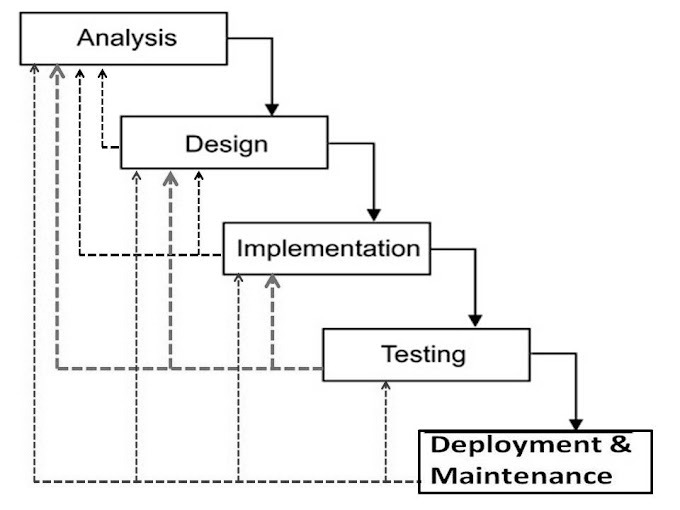
\includegraphics[width=0.6\textwidth]{Images/01 Life_cycle.jpg}  
    \caption{Iterative Waterfall Model}
    \label{Iterative Waterfall Model}  % Label for referencing the figure
\end{figure}


\subsection{Dependencies and Milestones} 
\noindent
Key dependencies were identified for successful project progression. For instance, completion of the data preparation phase was critical before proceeding to model development. Milestones were established at the end of each phase to ensure accountability and track progress. The successful completion of the requirement gathering phase marked the first milestone, followed by the data preparation phase, and so on.

\subsection{Scheduling}
\noindent
Effective scheduling is crucial to the success of any project, as it establishes a clear timeline for tasks, milestones, and dependencies. In the context of our project on detecting mental health disorders through social media analysis, a detailed schedule has been developed to guide the project from inception to completion. This schedule includes specific tasks such as requirement gathering, data preprocessing, model implementation, testing, and deployment, each with clearly defined deadlines. The iterative nature of our chosen methodology allows for flexibility within the schedule, enabling adjustments based on testing outcomes and stakeholder feedback. Key milestones, such as the completion of data analysis, model validation, and user acceptance testing, have been identified to monitor progress and ensure timely delivery of the final product. By utilizing project management tools, such as Microsoft Project, we can visualize and track the progress of tasks, manage resources effectively, and maintain open communication among team members, ensuring that the project stays on schedule and meets its objectives. This proactive approach to scheduling enhances our ability to deliver a high-quality solution that aligns with our goals and stakeholder expectations.

% Insert MS Project Plan Image
\begin{figure}[h!]  
    \centering
    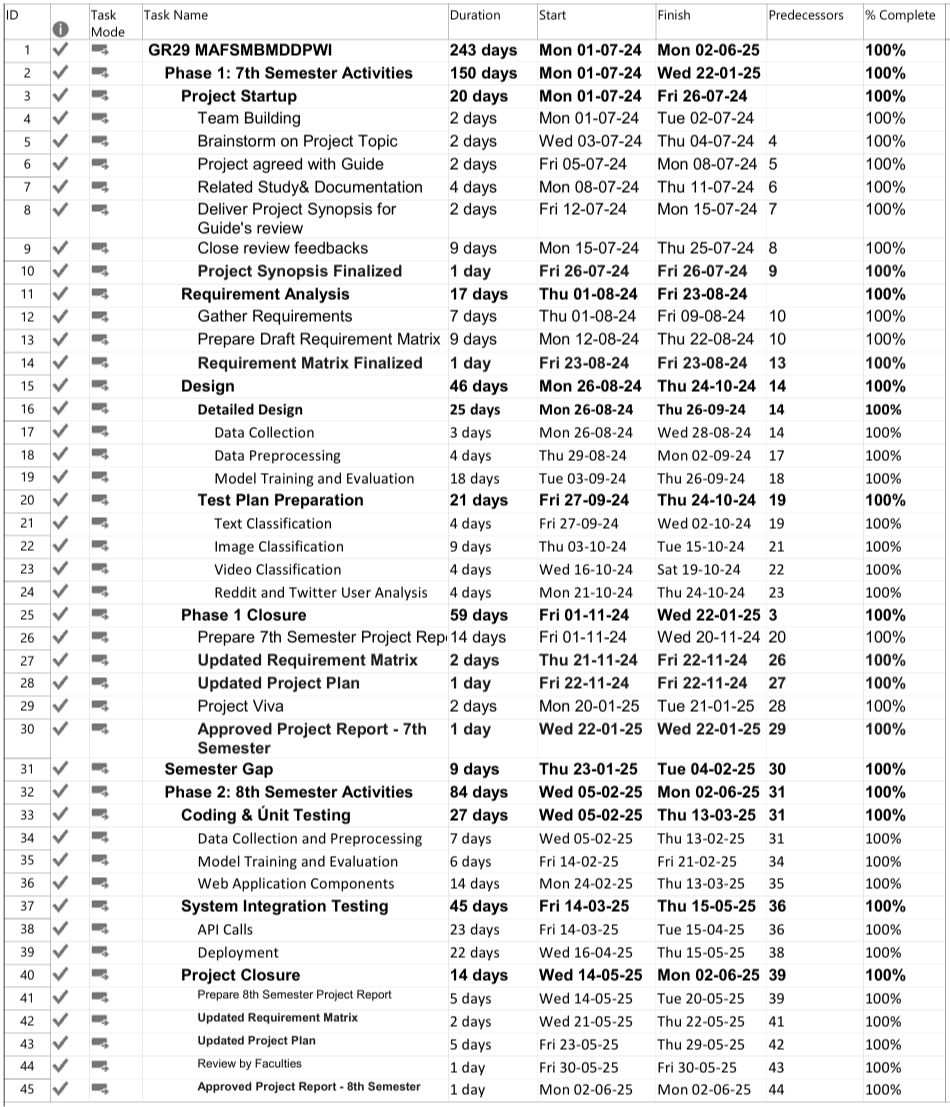
\includegraphics[width=0.9\textwidth]{Images/MS Project Plan Sem 7.png}  
    \caption{Project Plan}
    \label{Project Plan}  % Label for referencing the figure
\end{figure}

\vspace{2cm}

\begin{figure}[h!]  
    \centering
    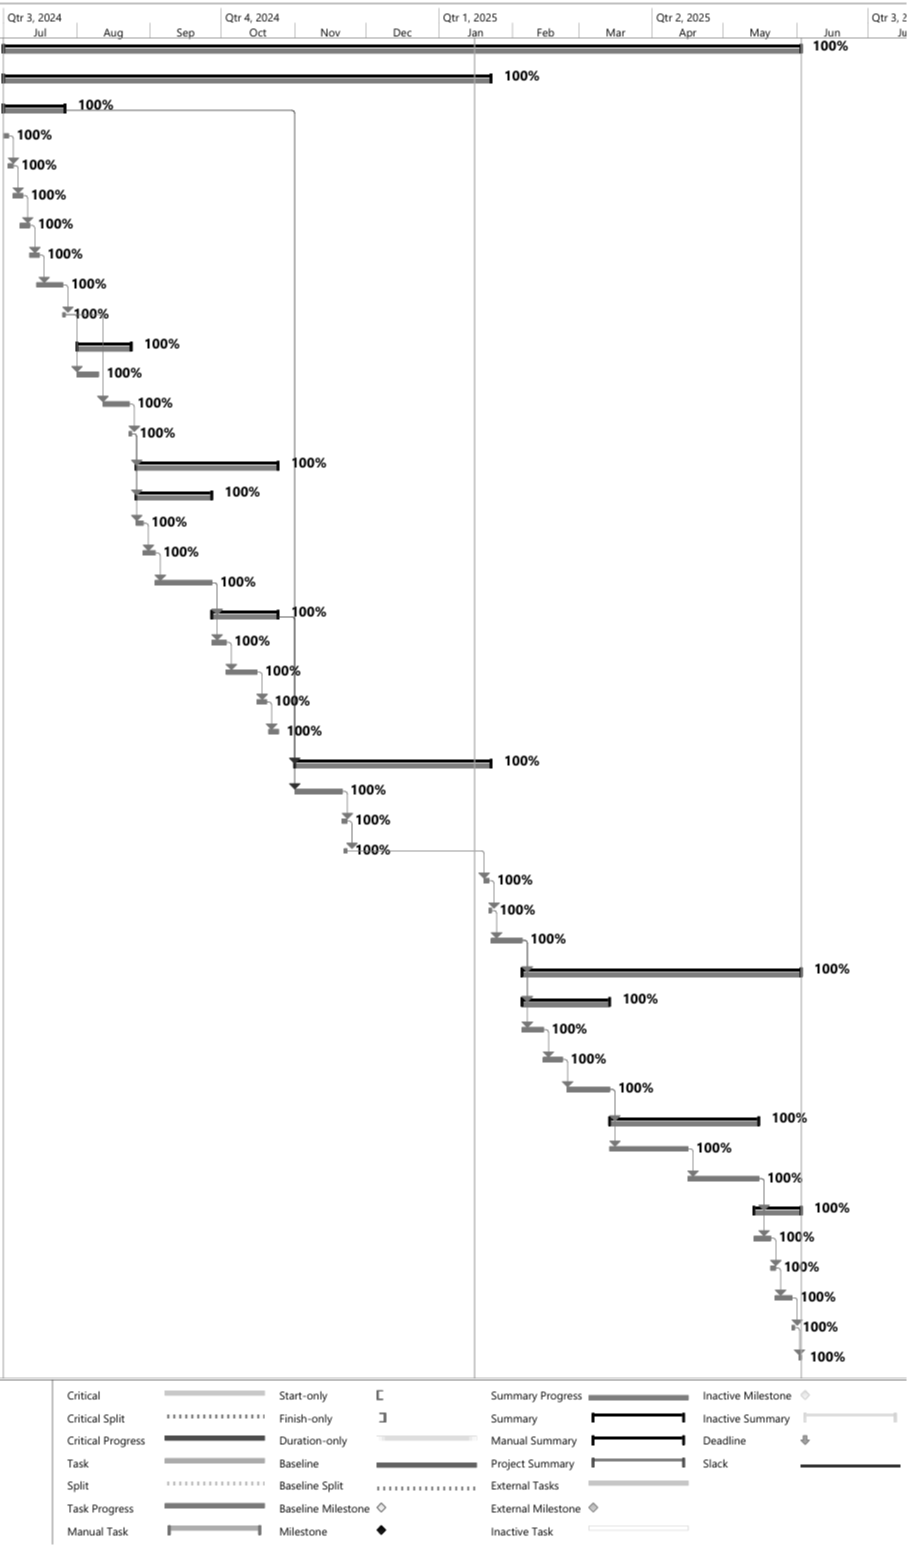
\includegraphics[width=0.9\textwidth]{Images/Gantt Chart.png}  
    \caption{Gantt Chart}
    \label{Gantt Chart}  % Label for referencing the figure
\end{figure}

% ----------------------- Project Planning ends ------------------------------


% --------------------- Requirement Analysis ---------------------------------

\section{Requirement Analysis}

\subsection{Requirement Matrix}
% For Requirement Matrix, latest excel should be pasted and formatted here.
\begin{figure}[h!]  
    \centering
    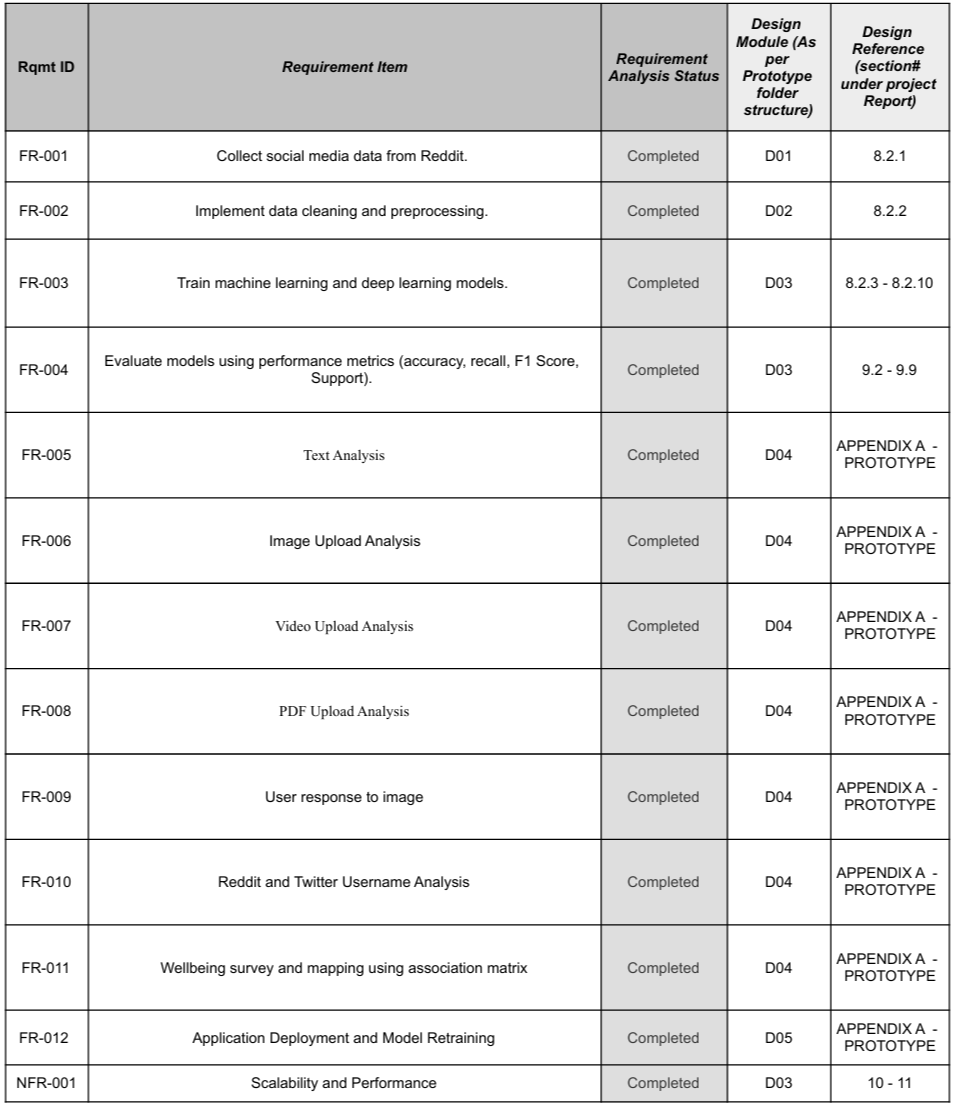
\includegraphics[width=1.0\textwidth]{Images/Requirement Matrix.png}  
    \caption{Requirement Matrix}
    \label{Requirement Matrix}  % Label for referencing the figure
\end{figure}

\noindent
The Requirement Matrix is a comprehensive tool used to track and manage the key requirements of a project. It systematically organizes each requirement with a unique identifier, description, priority, and category (such as functional or non-functional). The matrix also records the source of the requirement, its current status (e.g., in progress, completed), any dependencies on other requirements, and the team or individual responsible for fulfilling it. Additionally, it includes a verification method to ensure the requirement is met, such as through testing or review. This structured format helps ensure that all requirements are clearly defined, prioritized, and tracked, enabling effective project management and ensuring alignment with stakeholder expectations.

\subsection{Requirement Elaboration}
% Create separate sections for separate areas of requirement as in Requirement Matrix. 
% \vspace{.1in}

% \noindent
% For \textbf{Requirement Elaboration}, titles of s6.2.1, 6.2.2 etc. should be with the name of respective requirement areas. Your focus should be on: “What is needed in the system?” Requirement IDs should match with the ID column under Requirement Matrix.

\subsubsection{Functional Requirements}

\noindent
\textbf{\emph{Requirement ID: FR-001}} \\ 
\textbf{\emph{Description: Data Collection}} \\
\textbf{\emph{Priority: High}} \\
\textbf{\emph{Category: Functional}} \\
\noindent
The system requires an ability to collect and ingest a large dataset of Twitter sentiment data from Kaggle. The data should include text content from tweets, associated sentiment labels, and other metadata such as timestamp and user details. This will serve as the primary source of information for sentiment analysis and mental health disorder detection. The system must ensure that the dataset is loaded correctly into the machine learning environment, and any discrepancies in the structure should be handled with pre-processing steps like cleaning, normalization. \\

\noindent
\textbf{\emph{Requirement ID: FR-002}} \\ 
\textbf{\emph{Description: Data Cleaning and Preprocessing}} \\
\textbf{\emph{Priority: High}} \\
\textbf{\emph{Category: Functional}} \\
\noindent
The system must include modules to clean the raw data, such as removing irrelevant characters, handling missing data, and tokenizing text. For the social media posts, it is essential to remove URLs, stopwords, and unnecessary punctuation. The pre-processing pipeline should also convert the text into a suitable numerical format, such as Bag of Words (BoW) or Term Frequency-Inverse Document Frequency (TF-IDF), for further analysis. Proper pre-processing ensures that the data is in a form that can be efficiently used by machine learning models. \\

\noindent
\textbf{\emph{Requirement ID: FR-003}} \\ 
\textbf{\emph{Description: Sentiment and Disorder Detection Model}} \\
\textbf{\emph{Priority: High}} \\
\textbf{\emph{Category: Functional}} \\
\noindent
The system needs to implement machine learning algorithms such as k-Nearest Neighbors (k-NN) and Support Vector Machines (SVM) to classify social media posts based on their sentiment (positive, negative, neutral) and detect potential signs of mental health disorders. The system must be able to train these models on historical data and then apply them to predict the sentiment and detect mental health-related issues in new posts. \\

\noindent
\textbf{\emph{Requirement ID: FR-004}} \\ 
\textbf{\emph{Description: Model Validation and Evaluation}} \\
\textbf{\emph{Priority: High}} \\
\textbf{\emph{Category: Functional}} \\
\noindent
The system must evaluate the performance of the trained models by splitting the dataset into training and test sets. Various performance metrics like accuracy, precision, recall, and F1-score should be computed to assess the model’s effectiveness in detecting mental health disorders. Based on the evaluation, the system should allow for model fine-tuning, such as adjusting hyperparameters, to improve the overall performance. 


\subsubsection{Non Functional Requirements}

\noindent
\textbf{\emph{Requirement ID: NFR-001}} \\ 
\textbf{\emph{Description: Documentation}} \\
\textbf{\emph{Priority: Medium}} \\
\textbf{\emph{Category: Non Functional}} \\
\noindent
The addition of documentation and maintenance manuals as a non-functional requirement ensures that the system is not only usable in the short term but also maintainable and extensible over time. This guarantees that future updates and improvements to the system can be implemented without disrupting existing functionality or requiring a steep learning curve for new developers or users. \\

\noindent
\textbf{\emph{Requirement ID: NFR-002}} \\ 
\textbf{\emph{Description:  Scalability}} \\
\textbf{\emph{Priority: Medium}} \\
\textbf{\emph{Category: Non Functional}} \\
\noindent
The system must be designed to efficiently process large volumes of data, considering the potential growth in the amount of social media posts that need to be analyzed. The data processing pipeline should be scalable to handle increasing data size without significant degradation in performance. This could involve implementing parallel processing techniques or leveraging cloud-based infrastructure to ensure that processing large datasets remains feasible even as the dataset scales. 


% -------------------- Requirement Analysis Ends -----------------------------



% ----------------------------- Design ---------------------------------------

\section{Design}

\subsection{Technical Environment}
% Mention minimum hardware configuration, software tools and package details.
\noindent
The technical environment for the project "Analyzing Social Media Posts for Mental Health Disorder Detection" comprises a combination of hardware, software, and tools that enable smooth data analysis, machine learning model training, and deployment. Below is a detailed overview of the minimum hardware configuration, software tools, and package details necessary to carry out this project effectively. \\

\noindent
\textbf{Minimum Hardware Configuration} \\
\noindent
Given the nature of the project, which involves processing textual data and training machine learning models, the hardware requirements are modest but significant enough to ensure optimal performance. The minimum configuration needed is:
\begin{itemize}
    \item \textbf{Processor} :
    \noindent
    Intel Core i5 (or equivalent) with a base clock speed of at least 2.5 GHz. A multi-core processor is preferred as it helps in parallel processing, which is essential during model training and data preprocessing steps.
    \item \textbf{RAM} :
    \noindent
    8 GB of RAM is recommended to handle the operations of data loading, cleaning, and transformation. Large datasets, like those used in this project, may require more memory to prevent memory overflow errors and reduce delays during processing. For larger datasets, 16 GB of RAM would be ideal.
    \item \textbf{Storage} :
    \noindent
    At least 256 GB of SSD storage is recommended. Faster storage access significantly impacts loading time for datasets and dependencies. SSD is preferred over traditional HDD because of its faster read/write speeds, which benefit large datasets like the Reddit-based social media posts used in this project.
    \item \textbf{Graphics Processing Unit (GPU)} :
    \noindent
    For basic machine learning tasks like Logistic Regression or SVM, a dedicated GPU is not necessary. However, if deep learning models or more complex neural networks were introduced later, a GPU like NVIDIA GTX 1060 with 4 GB VRAM or higher would be advantageous.
    \item \textbf{Operating System} :
    \noindent
    Windows 10 (64-bit) or higher, macOS 10.13 (High Sierra) or higher, or any stable Linux distribution (e.g., Ubuntu 18.04 or higher). The operating system should support all necessary machine learning libraries and be compatible with the tools required for the project.
\end{itemize} \\

\noindent
\textbf{Software Tools and Packages} \\
\noindent
For the software stack, the project leverages a set of well-established tools, platforms, and programming libraries to ensure smooth execution from data preprocessing to model deployment:
\begin{itemize}
    \item \textbf{Python} :
    \noindent
    The primary programming language used for data processing, model training, and evaluation. Python is chosen due to its rich ecosystem of libraries and frameworks tailored for machine learning and data science.
    \item \textbf{Google Colab} :
    \noindent
    A cloud-based platform used for writing, executing, and sharing Python code. Google Colab provides free access to GPU and TPU resources, which is beneficial for intensive model training tasks. It also offers seamless integration with libraries like TensorFlow and PyTorch.
    \item \textbf{Jupyter Notebooks} :
    \noindent
     An alternative environment for running Python code, offering an interactive interface to write and execute code in blocks. It allows for easy visualization of results and is highly suitable for collaborative projects.
\end{itemize}

\pagebreak

\noindent
\textbf{Python Packages and Libraries}
\begin{table}[h!]
\centering
\begin{tabular}{|p{9cm}|p{6cm}|}
  \hline
  \multicolumn{1}{|c|}{\textbf{Package}} & \multicolumn{1}{c|}{\textbf{Purpose}} \\
  
  \hline
  \texttt{praw} & Access Reddit posts for data collection. \\
  
  \hline
  \texttt{pandas} & Data manipulation and analysis. \\
  
  \hline
  \texttt{textblob} & Text processing and sentiment analysis. \\
  
  \hline
  \texttt{time} & Managing execution time. \\
  
  \hline
  \texttt{re} & Regular expressions for text cleaning. \\
  
  \hline
  \texttt{TfidfVectorizer} & Convert text to TF-IDF features. \\
  
  \hline
  \texttt{stopwords} & Remove stopwords from text. \\
  
  \hline
  \texttt{tokenize} & Tokenize text data. \\
  
  \hline
  \texttt{nltk} & Natural Language Toolkit for text processing. \\
  
  \hline
  \texttt{CountVectorizer} & Convert text to Bag-of-Words features. \\
  
  \hline
  \texttt{split} & Split the dataset into training and testing sets. \\
  
  \hline
  \texttt{LogisticRegression} & Build and train Logistic Regression models. \\
  
  \hline
  \texttt{sklearn.metrics.accuracy\_score} & Calculate accuracy of the model. \\
  
  \hline
  \texttt{report} & Generate classification performance report. \\
  
  \hline
  \texttt{RandomizedSearchCV} & Hyperparameter tuning for models. \\
  
  \hline
  \texttt{seaborn} & Data visualization and plotting. \\
  
  \hline
  \texttt{matplotlib.pyplot} & Create and customize plots. \\
  
  \hline
  \texttt{matrix} & Generate confusion matrix. \\
  
  \hline
  \texttt{roc\_curve, auc, roc\_auc\_score} & Evaluate model’s ROC and AUC scores. \\
  
  \hline
  \texttt{KNeighborsClassifier} & Build k-Nearest Neighbors (k-NN) models. \\
  
  \hline
  \texttt{svm.SVC} & Build Support Vector Machines (SVM) models. \\
  
  \hline
  \texttt{naive\_bayes.MultinomialNB} & Build Naive Bayes models. \\
  
  \hline
  \texttt{scipy.stats.uniform} & Statistical operations for tuning models. \\
  
  \hline
  \texttt{RandomForestClassifier} & Build Random Forest models. \\
  
  \hline
  \texttt{sklearn.preprocessing.label\_binarize} & Convert labels for multi-class ROC analysis. \\
  
  \hline
\end{tabular}
\end{table}



\pagebreak

\subsection{Hierarchy of Modules}
% Provide a diagram.
\begin{figure}[h!]  
    \centering
    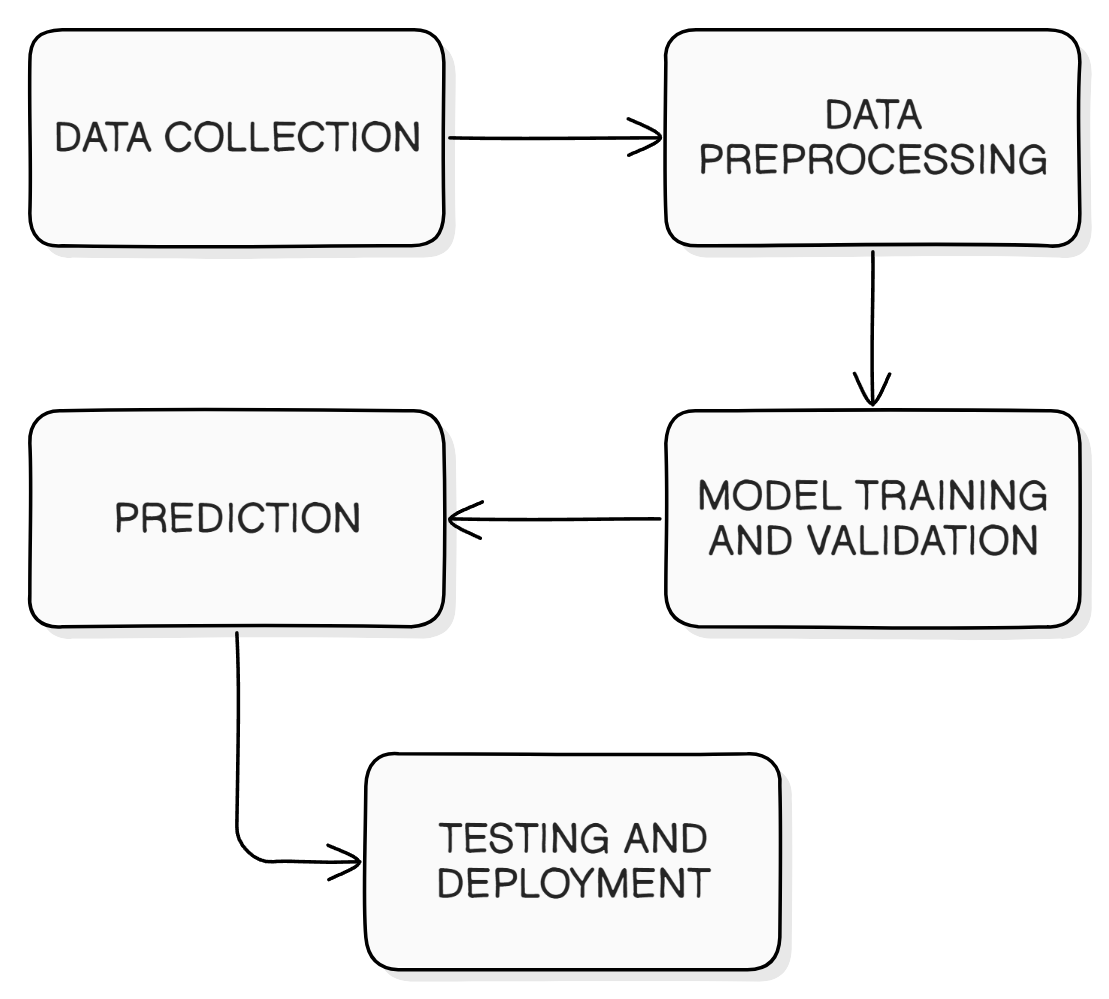
\includegraphics[width=0.6\textwidth]{Images/Project Modules.png}  
    \caption{Project Modules}
    \label{Project Modules}  % Label for referencing the figure
\end{figure}

\noindent
In this project, the system is organized into several key modules to efficiently classify mental health issues based on text input. The Data Loading and Preprocessing Module is responsible for loading the CSV data from preprocessed\_mental\_health\_text.csv and performing essential text cleaning operations, such as tokenization and stop-word removal, to prepare the data for analysis. Following this, the Feature Extraction Module employs techniques like Bag of Words or TF-IDF to convert the cleaned text into numerical features suitable for classification. The Model Training and Validation Module takes these features, splitting the dataset into training and testing sets, and implements multiple machine learning models, including Logistic Regression, k-Nearest Neighbors (k-NN), Support Vector Machines (SVM), Naive Bayes, and Random Forest. Each model is evaluated using relevant metrics to assess accuracy and performance. The Prediction Module is designed to accept new input text and utilize the trained models to predict mental health issues, ensuring that various perspectives from the different algorithms are considered. Finally, the Deployment Module offers a free solution for serving the models, potentially utilizing platforms like Google Colab or Hugging Face, allowing for real-time predictions in practical applications.

\subsection{Detailed Design}
% Provide hierarchy of modules or overall system diagram. 
% \vspace{.1in}
\begin{figure}[h!]  
    \centering
    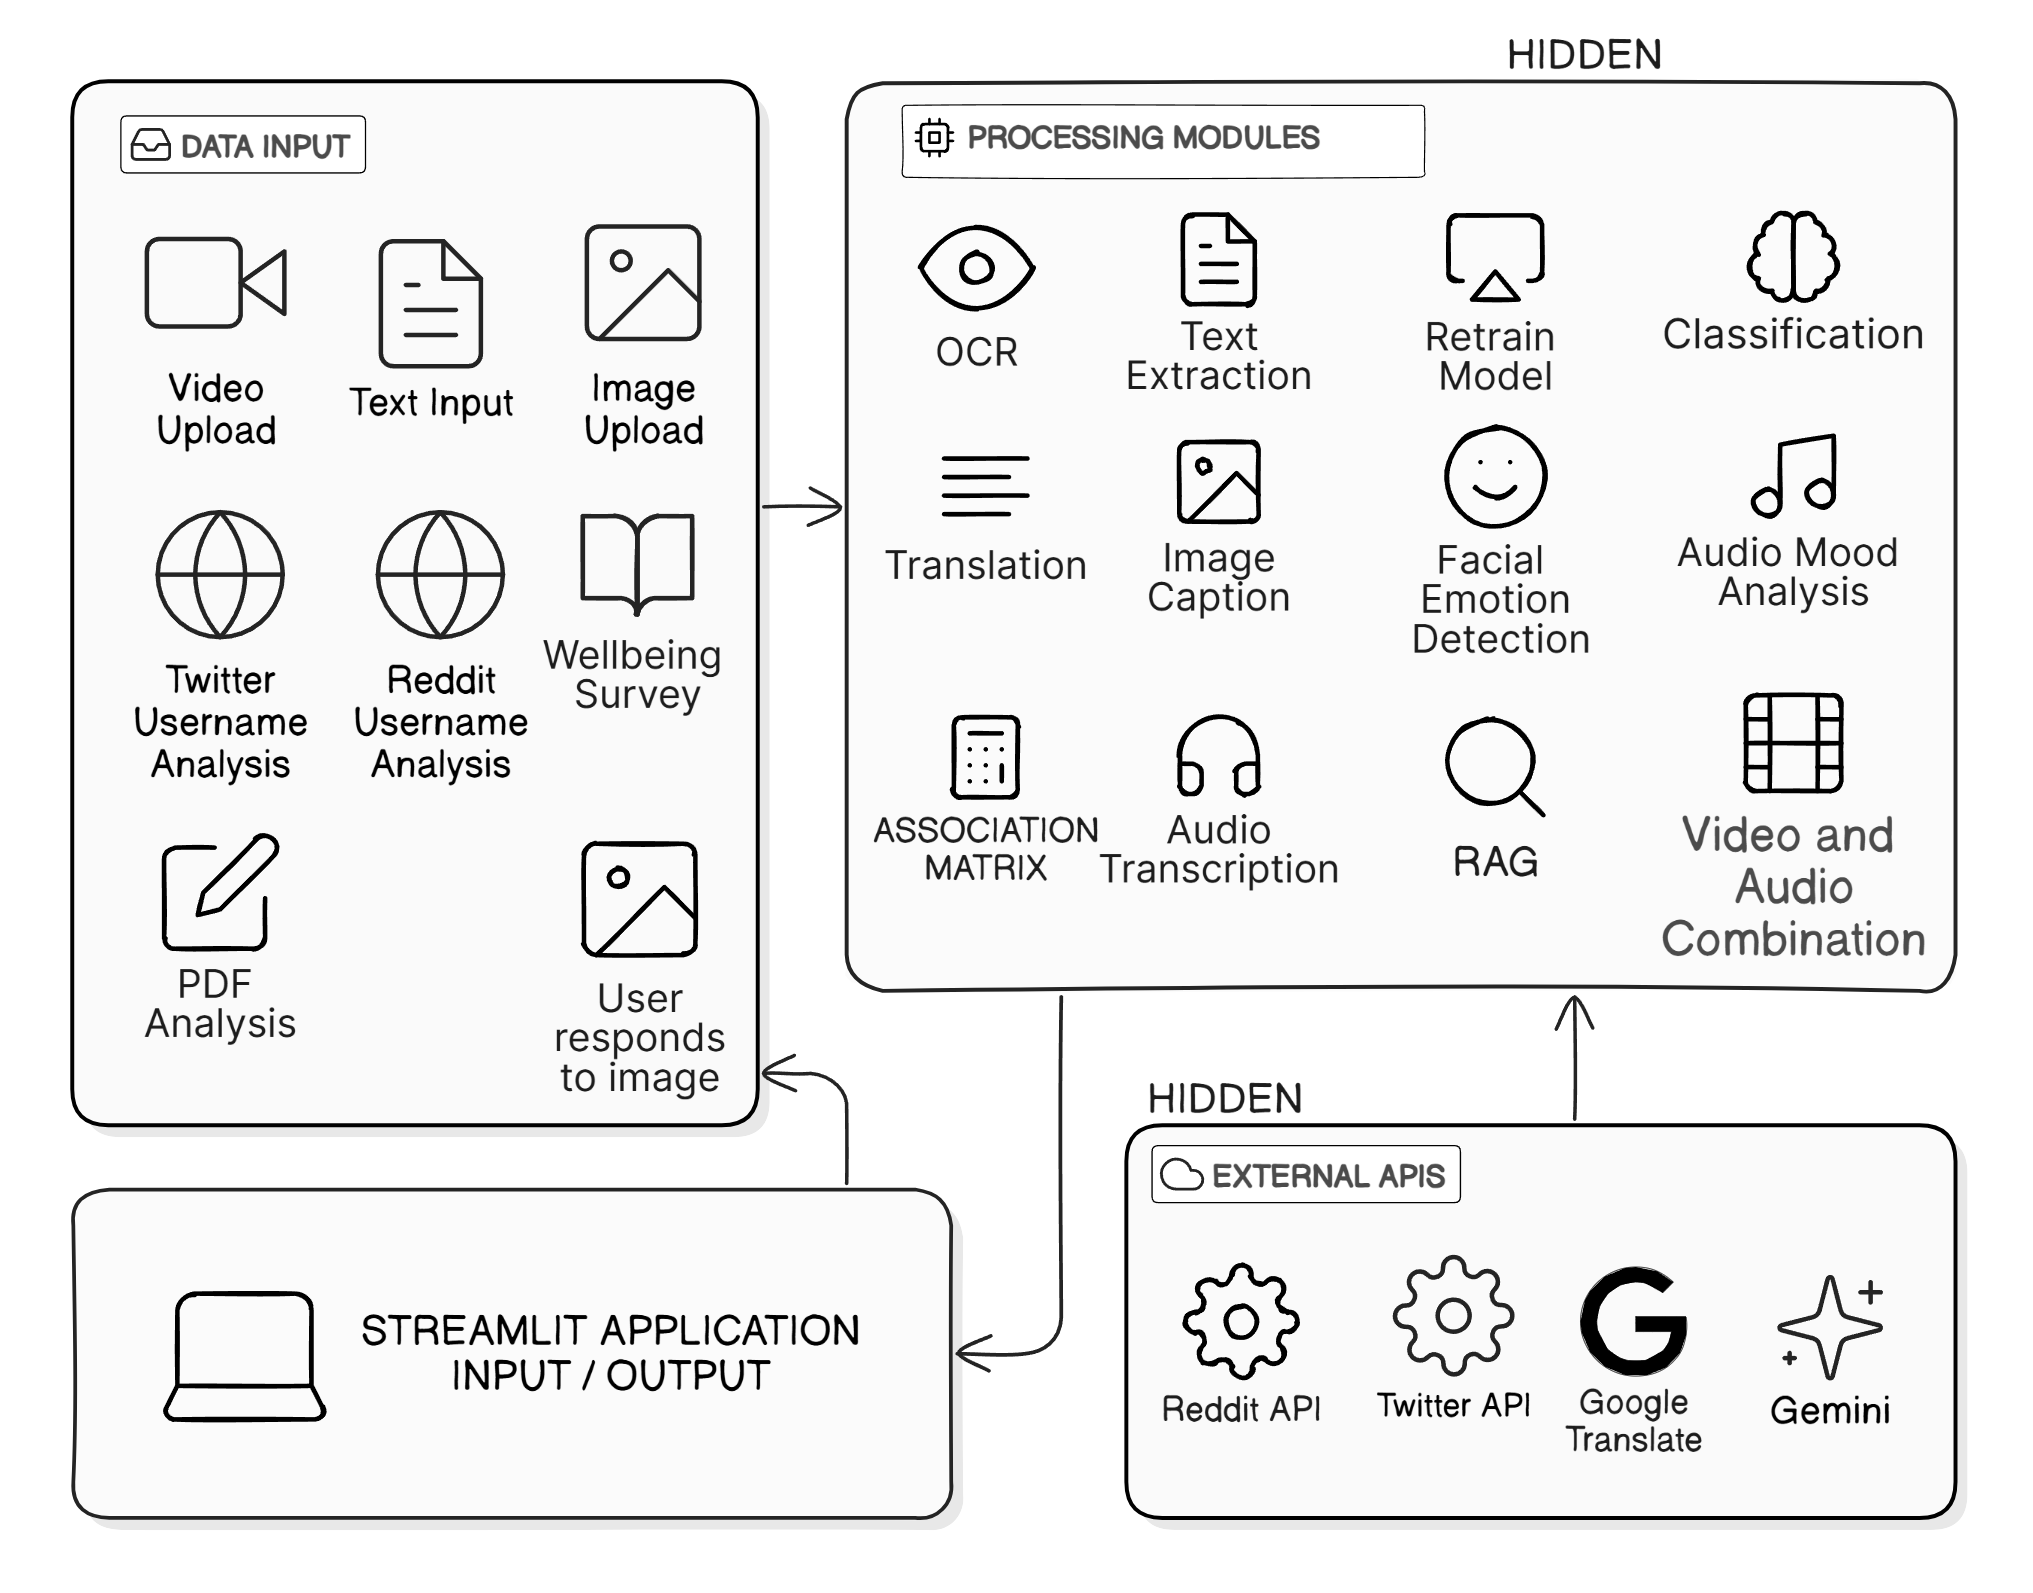
\includegraphics[width=1.0\textwidth]{Images/System Overview.png}  
    \caption{System Overview}
    \label{System Overview}  % Label for referencing the figure
\end{figure}

\begin{figure}[h!]  
    \centering
    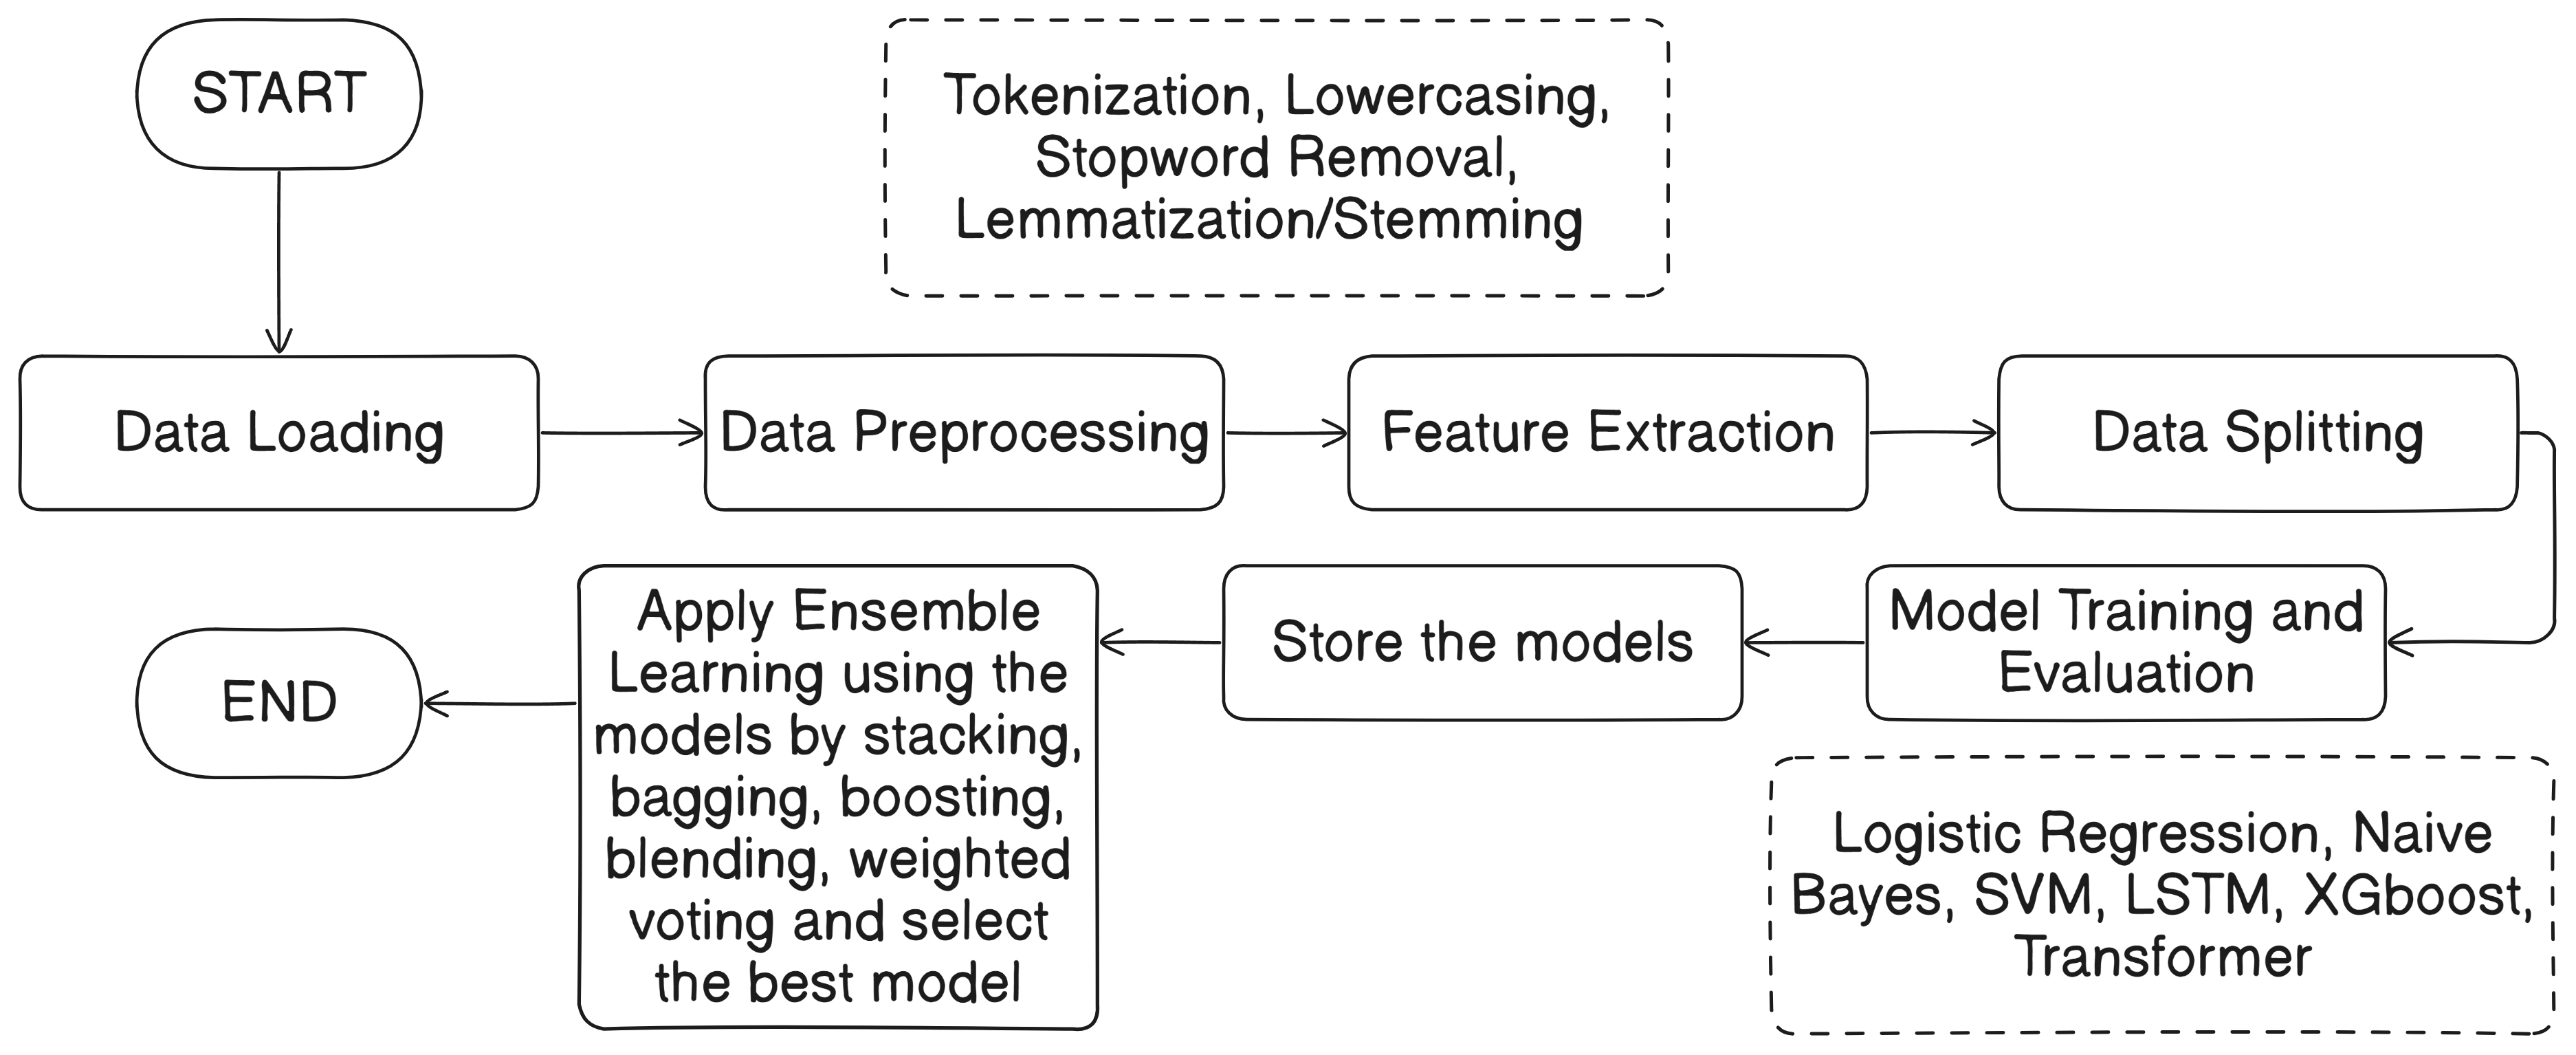
\includegraphics[width=0.95\textwidth]{Images/ML Model Workflow.png}  
    \caption{Model Workflow}
    \label{Model Workflow}  % Label for referencing the figure
\end{figure}

% \noindent
% For Detailed Design, use flowcharts, DFD, UML or ER diagrams as applicable. Titles of s7.2.1, 7.2.2 etc. should be with the name of respective design modules. Your focus should be on: “How the requirement will be implemented in the system?” Design Reference subsection numbers should be matching as stated in Requirement Matrix.
\vspace{.1in}

\subsubsection{Data Loading and Preprocessing}
\noindent
The Data Loading and Preprocessing Module is the foundation of the system, responsible for ingesting and preparing the text data for analysis. This module begins by loading the dataset from the preprocessed\_mental\_health\_text.csv file, which contains various mental health-related text entries. Once the data is loaded, a series of preprocessing steps are conducted to ensure the text is clean and ready for feature extraction. This includes tokenization, where the text is split into individual words or tokens, and lowercasing to maintain uniformity across the dataset. Additionally, stop-word removal is performed to eliminate common words that do not contribute to the meaning, such as "and," "the," and "is." Finally, lemmatization or stemming is applied to reduce words to their base or root forms. These preprocessing techniques are crucial as they help improve the quality of the input data, ultimately leading to better model performance.

\subsubsection{Feature Extraction}
\noindent
In the Feature Extraction Module, the preprocessed text data is transformed into a numerical format that machine learning algorithms can process. This module allows for the selection between two primary feature extraction methods: Bag of Words (BoW) and Term Frequency-Inverse Document Frequency (TF-IDF). The Bag of Words model creates a representation of the text based on the frequency of words, disregarding the order in which they appear, which simplifies the input for classification algorithms. Alternatively, the TF-IDF approach evaluates the importance of words in the dataset by considering their frequency in individual documents relative to their overall occurrence across all documents. This helps in highlighting the most informative words. By converting text into numerical features, this module prepares the data for the subsequent training and validation stages, ensuring that the classification models can effectively interpret the input.

\subsubsection{Model Training and Validation}
\noindent
The Model Training and Validation Module is critical to developing a robust classification system. In this module, the dataset is split into training and testing sets to evaluate the performance of the models accurately. Various classification algorithms are employed, including Logistic Regression, k-Nearest Neighbors (k-NN), Support Vector Machines (SVM), Naive Bayes, and Random Forest. Each model is trained on the training set, which involves adjusting the model parameters based on the input features and their corresponding labels. Following training, the models undergo validation to assess their performance using various metrics such as accuracy, precision, recall, and F1-score. A decision point is included to determine if the achieved accuracy meets the project requirements. If the accuracy is deemed acceptable, the model proceeds to the deployment stage. 

\begin{figure}[h!]  
    \centering
    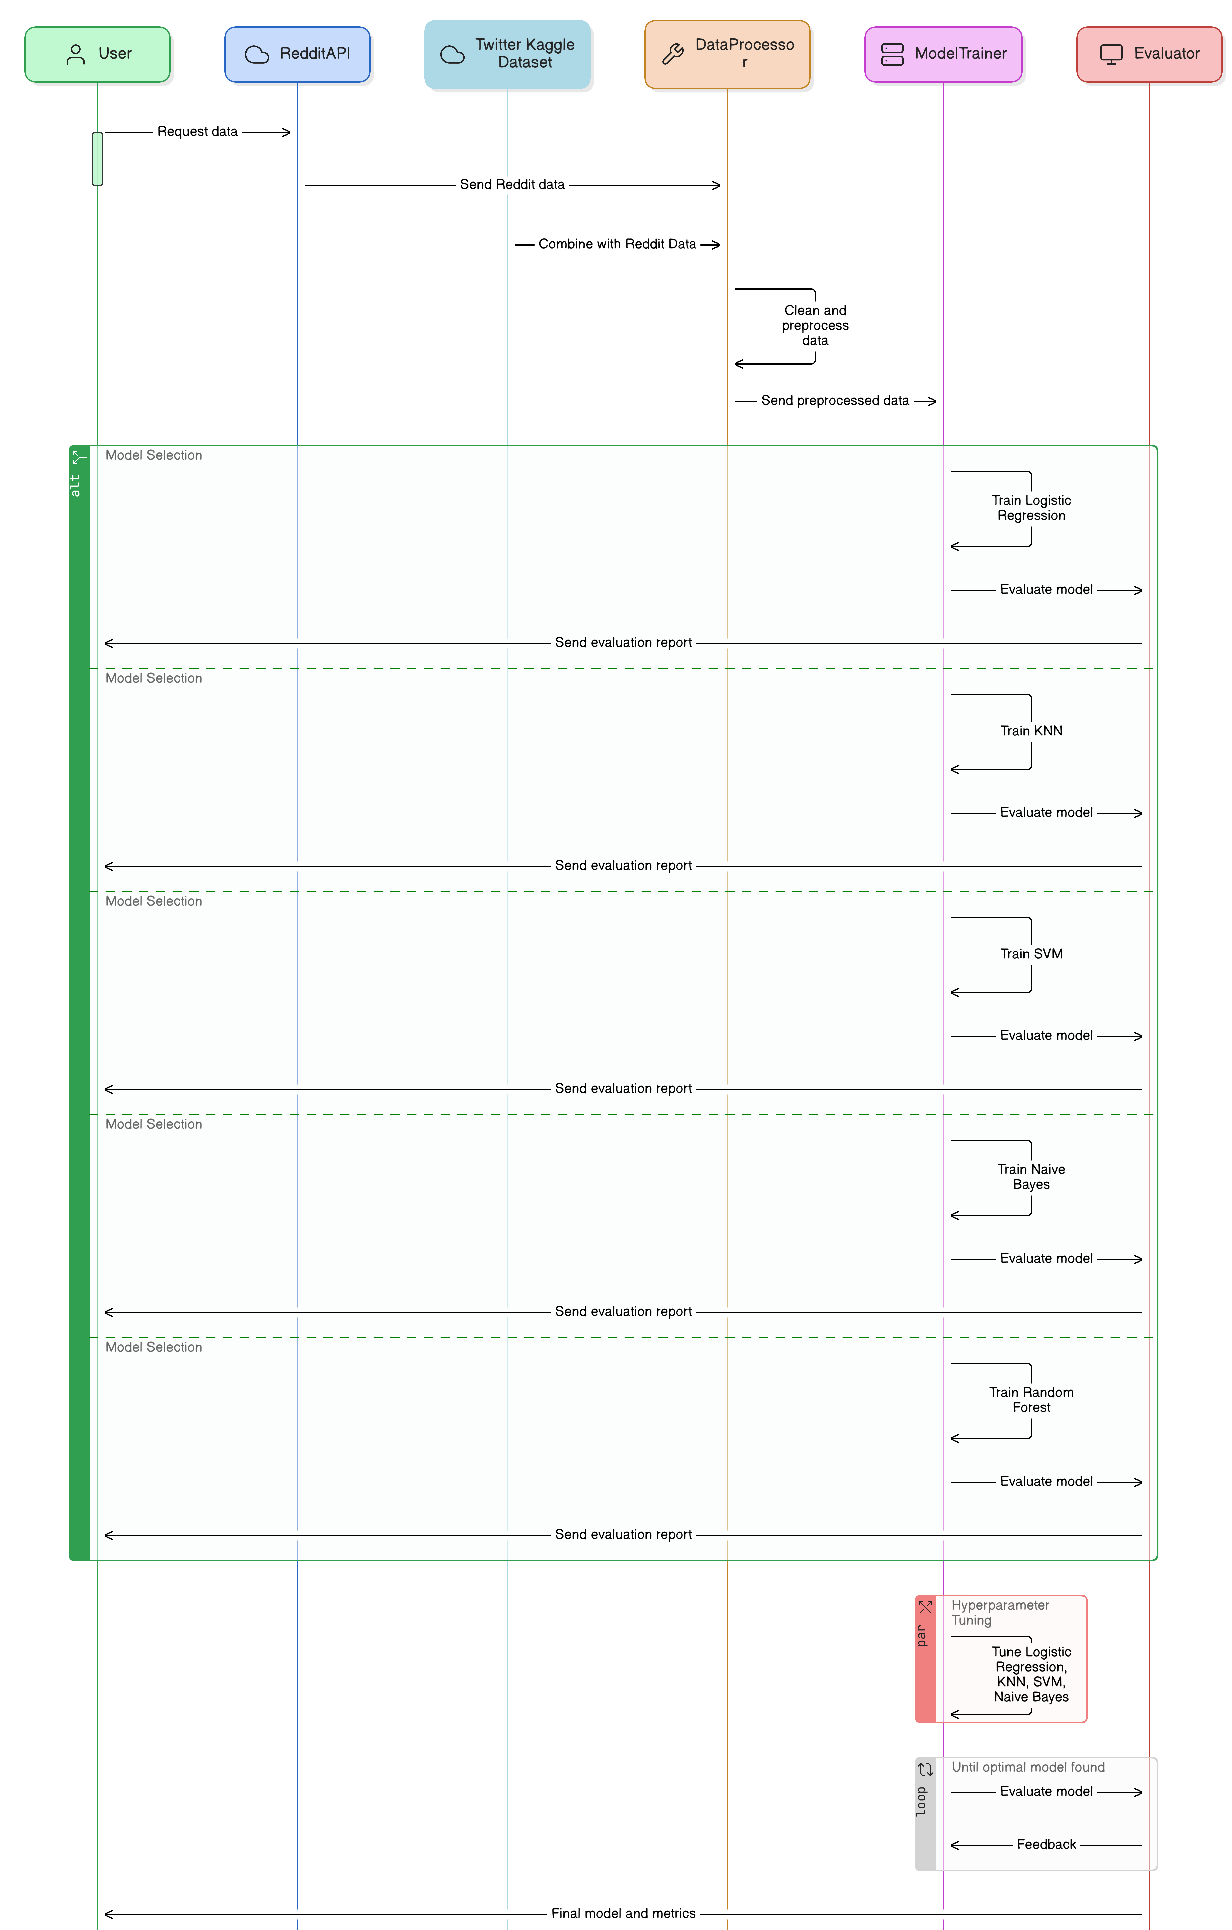
\includegraphics[width=0.85\textwidth]{Images/Project Sequence.png}  
    \caption{Project Sequence}
    \label{Project Sequence}  % Label for referencing the figure
\end{figure}

\subsubsection{Prediction}
\noindent
The Prediction Module is designed to provide real-time classification of new input text related to mental health issues. Upon receiving user input, this module initiates a preprocessing workflow that mirrors the steps applied during the training phase, including tokenization, lowercasing, stop-word removal, and lemmatization or stemming. Once the input text is preprocessed, it is fed into the trained classification models to generate predictions. Each model may provide a classification result, allowing for a comprehensive analysis of the input. This module not only delivers the predicted mental health issue but also ensures that users receive an informative output that reflects the confidence level of each prediction, enabling them to understand the model's reasoning. The seamless integration of this module into the overall system enhances the user experience by providing instant and relevant feedback.

\subsubsection{Deployment}
\noindent
The Deployment Module focuses on making the trained models accessible for real-time predictions. Once the models have been validated and selected based on their performance, this module prepares them for deployment on suitable platforms, such as Google Colab or Hugging Face. This involves packaging the models and creating a user interface where users can input text and receive predictions. The deployment process also includes considerations for scaling, ensuring that the system can handle multiple requests simultaneously while maintaining responsiveness. By providing a free and efficient deployment solution, this module enables users to access the mental health classification service easily. The deployment of the models ensures that the insights generated from the analysis can be utilized effectively in real-world applications, contributing to better mental health awareness and support.

% \noindent
% Create separate sections for separate modules of design as in Requirement Matrix. Ensure to provide Design Diagrams \textit{(e.g. System overview / DFDs / ERDs etc.; cross-reference to be drawn from Chapter 6), Decision matrix (for algorithm recommendation etc.) }




% \subsubsection{Name of Design Module 1 \label{sec:design_mod1}}
% \subsubsection{Name of Design Module 2 \label{sec:design_mod2}}
% \subsubsection{Name of Design Module 3 etc \label{sec:design_mod3}}


% Refer APPENDIX A  – Prototypes \ref{sec:proto} for prototype details.


% ------------------------------ Design Ends ---------------------------------


% --------------------------- Implementation ---------------------------------

\section{Implementation}
%Focus of 7\textsuperscript{th} semester deliverables are analysis, design and prototyping. Refer APPENDIX A – Prototypes for prototype details.
% For Test Planning, s6.4 should contain the Test Plan in tabular format, where each Test
% Case should be represented with distinct id, prefixed with ``T-$<<$module$>>$-'', where module represents the short code of the respective design module. 
% Test Case numbers should be matching as stated in Requirement Matrix.

\subsection{Features From RM}
\noindent
For the initial prototype development, a subset of the requirements from the Requirement Matrix (RM) was carefully selected to focus on implementing core functionalities and demonstrating proof of concept. The selection was based on a combination of high-priority functional requirements that form the backbone of the system, ensuring that critical features are built and validated before expanding the scope.

The requirements chosen for the prototype primarily involve data preprocessing, model training, and evaluation processes. These requirements were selected because they are fundamental to the project's success, ensuring that the data pipeline and model implementation work seamlessly together. This subset of features lays the groundwork for later integration with additional components and more complex functionality.

The filtered part of the RM focuses on the following high-priority requirements: data cleaning and feature extraction, training of machine learning models, and evaluation of model performance using standard metrics. These requirements were identified as crucial because they directly impact the system's ability to handle data, learn patterns, and provide meaningful outputs. Without successfully implementing these core features, the overall effectiveness of the solution would be significantly reduced.

Furthermore, these selected features align with the project’s goals and provide a clear pathway for incremental development. By narrowing down the requirements to these foundational aspects, the development team can ensure that the prototype is not only functional but also extensible, providing a robust framework for future enhancements.

\begin{figure}[h!]  
    \centering
    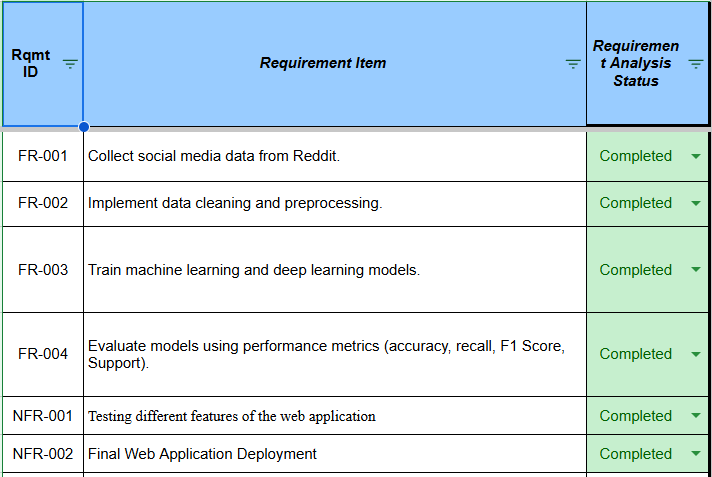
\includegraphics[width=0.85\textwidth]{Images/RM_part_for_implementation.png}  
    \caption{Features from Requirement Matrix}
    \label{Features from Requirement Matrix}  % Label for referencing the figure
\end{figure}

\subsection{Steps of Compilation, Execution and Setup}
\begin{enumerate}
    \item \textbf{Setup the Development Environment}
    \begin{itemize}
        \item Ensure Python 3.x is installed on your system.
        \item Install a virtual environment package if not already available:
        \begin{verbatim}
        pip install virtualenv
        \end{verbatim}
        \item Create a virtual environment for the project:
        \begin{verbatim}
        python -m venv project_env
        \end{verbatim}
        \item Activate the virtual environment:
        \begin{itemize}
            \item For Windows:
            \begin{verbatim}
            .\project_env\Scripts\activate
            \end{verbatim}
            \item For Linux/Mac:
            \begin{verbatim}
            source project_env/bin/activate
            \end{verbatim}
        \end{itemize}
    \end{itemize}

    \item \textbf{Install Required Libraries}
    \begin{itemize}
        \item Install the necessary Python libraries using the following command:
        \begin{verbatim}
        pip install pandas numpy scikit-learn matplotlib
        \end{verbatim}
        \item If your project has additional dependencies, include them as well:
        \begin{verbatim}
        pip install tensorflow keras seaborn
        \end{verbatim}
    \end{itemize}

    \item \textbf{Set Up the Project Directory}
    \begin{itemize}
        \item Organize your project directory as follows:
        \begin{verbatim}
        project_folder/
        ├── data/
        │   └── sample_data.csv
        ├── notebooks/
        │   └── project_prototype.ipynb
        ├── src/
        │   └── main.py
        └── requirements.txt
        \end{verbatim}
        \item Place your input data files in the \texttt{data/} folder.
        \item Store Jupyter notebooks in the \texttt{notebooks/} folder.
        \item Add the main code files in the \texttt{src/} folder.
    \end{itemize}

    \item \textbf{Configure the Jupyter Notebook Environment}
    \begin{itemize}
        \item Navigate to the \texttt{notebooks/} folder using the command line:
        \begin{verbatim}
        cd notebooks
        \end{verbatim}
        \item Launch Jupyter Notebook:
        \begin{verbatim}
        jupyter notebook
        \end{verbatim}
        \item Open the \texttt{project\_prototype.ipynb} file from the Jupyter interface and execute each cell sequentially to run the prototype.
    \end{itemize}

    \item \textbf{Compilation and Execution of the Main Code (If Using Scripts)}
    \begin{itemize}
        \item If you are running the project using a script (e.g., \texttt{main.py}), navigate to the \texttt{src/} folder:
        \begin{verbatim}
        cd ../src
        \end{verbatim}
        \item Run the main script:
        \begin{verbatim}
        python main.py
        \end{verbatim}
        \item Ensure that the paths to the data files and other dependencies are correctly set in your code.
    \end{itemize}

    \item \textbf{Setup Test Data for Evaluation}
    \begin{itemize}
        \item Place the test dataset in the \texttt{data/} folder, ensuring it follows the format specified in the documentation.
        \item If using the command line, you can test with different data files by updating the file path in the code or using command-line arguments.
    \end{itemize}

    \item \textbf{View and Analyze the Output}
    \begin{itemize}
        \item For Jupyter Notebooks, observe the outputs directly in the notebook cells.
        \item If using scripts, the results (e.g., model performance, accuracy metrics, or visualizations) will be printed to the console or saved as files in the \texttt{output/} folder, depending on the implementation.
    \end{itemize}

    \item \textbf{Document and Verify the Execution}
    \begin{itemize}
        \item Document any issues or errors encountered during the compilation and execution.
        \item Perform a verification of results against the expected outputs to ensure correctness.
    \end{itemize}
\end{enumerate}

\subsection{Code Details and Output}

% Data Collection
\subsubsection{Data Collection: Scraping Reddit Posts}
\noindent
The code snippet below demonstrates how Reddit posts related to mental health issues are collected and preprocessed for further analysis. This process involves using the `praw` library to access the Reddit API, collecting posts from specified subreddits, extracting text data, calculating sentiment scores using `TextBlob`, and saving the processed data into a CSV file.

\begin{itemize}
    \item \textbf{Library Installation and Importation:}
    \begin{verbatim}
    !pip install praw
    import praw
    import pandas as pd
    from textblob import TextBlob
    import time
    \end{verbatim}
    \noindent
    The code starts by installing and importing necessary libraries: 
    \texttt{praw} (Python Reddit API Wrapper) for accessing Reddit data, 
    \texttt{pandas} for handling tabular data, 
    \texttt{TextBlob} for sentiment analysis, 
    and \texttt{time} for managing pauses during the scraping process to avoid rate limits.

    \item \textbf{Reddit API Authentication:}
    \begin{verbatim}
    reddit = praw.Reddit(client_id=<Reddit Client ID>,
                         client_secret=<Reddit Client Secret>,
                         user_agent='Mental Health')
    \end{verbatim}
    \noindent
    Here, the Reddit API credentials (`client\_id`, `client\_secret`, and `user\_agent`) are specified to create an authorized `praw.Reddit` object, which will be used to interact with Reddit.

    \item \textbf{Defining Subreddits to Scrape:}
    \begin{verbatim}
    subreddits = ['normal','depression','anxiety','bipolar','ptsd']
    \end{verbatim}
    \noindent
    The subreddits related to mental health are stored in a list named `subreddits`. These communities are targeted for data collection.

    \item \textbf{Setting Up Post Collection:}
    \begin{verbatim}
    post_types = ['hot', 'new', 'top']
    posts_per_type = 1500
    \end{verbatim}
    \noindent
    Three categories of posts are selected: `hot`, `new`, and `top`. The number of posts to be collected from each category is set to 1500.

    \item \textbf{Iterating through Subreddits and Post Types:}
    \begin{verbatim}
    for subreddit in subreddits:
        for post_type in post_types:
            if post_type == 'hot':
                subreddit_posts = reddit.subreddit(subreddit).
                hot(limit=posts_per_type)
            elif post_type == 'new':
                subreddit_posts = reddit.subreddit(subreddit).
                new(limit=posts_per_type)
            elif post_type == 'top':
                subreddit_posts = reddit.subreddit(subreddit).
                top(limit=posts_per_type)
    \end{verbatim}
    \noindent
    Nested loops are used to iterate through each subreddit and post type, creating a collection of posts from each combination.

    \item \textbf{Collecting and Labeling Data:}
    \begin{verbatim}
    for post in subreddit_posts:
        post_content = post.title + " " + post.selftext
        sentiment = TextBlob(post_content).sentiment.polarity
    \end{verbatim}
    \noindent
    Each post’s title and content are concatenated into a single string. Sentiment analysis is then performed using `TextBlob` to generate a polarity score, which ranges from -1 (negative) to 1 (positive).

    \item \textbf{Assigning Sentiment Labels:}
    \begin{verbatim}
    if sentiment > 0:
        sentiment_label = 1.0
    elif sentiment < 0:
        sentiment_label = -1.0
    else:
        sentiment_label = 0.0
    \end{verbatim}
    \noindent
    Based on the polarity score, a label is assigned: 1.0 for positive, -1.0 for negative, and 0.0 for neutral sentiment.

    \item \textbf{Storing Data with Labels:}
    \begin{verbatim}
    issue = subreddit
    data.append([post_content, sentiment_label, issue])
    \end{verbatim}
    \noindent
    Each post is associated with its respective subreddit label (mental health issue type) and stored in the `data` list.

    \item \textbf{Handling Rate Limits:}
    \begin{verbatim}
    time.sleep(2)
    \end{verbatim}
    \noindent
    A two-second delay is introduced after processing each type of post to avoid triggering Reddit’s rate limits.

    \item \textbf{Converting Data to DataFrame and Saving to CSV:}
    \begin{verbatim}
    df = pd.DataFrame(data, columns=['text', 'sentiment', 
    mental_health_issue'])
    df.to_csv('mental_health.csv', index=False)
    \end{verbatim}
    \noindent
    Finally, the collected data is converted into a `pandas` DataFrame with columns for text, sentiment, and mental health issue, and saved to a CSV file named `mental\_health.csv`.
\end{itemize}

% Genrating Final Dataset
\subsubsection{Generating the Final Dataset}

\noindent
The following code snippet combines two separate datasets—`mental\_health.csv` and `twitter\_mh.csv`—into a single CSV file named `mental\_health\_text.csv`. This step is crucial for consolidating different sources of mental health-related data into a unified dataset for further analysis.

\begin{verbatim}
import pandas as pd
\end{verbatim}

\noindent
The \texttt{pandas} library is imported as \texttt{pd}. It is a powerful library for data manipulation and analysis, allowing easy handling of structured data formats such as CSV files.

\begin{verbatim}
# Load the two CSV files
csv1 = pd.read_csv('mental_health.csv')
csv2 = pd.read_csv('twitter_mh.csv')
\end{verbatim}

\noindent
Here, the two CSV files, \texttt{mental\_health.csv} and \texttt{twitter\_mh.csv}, are read into separate \texttt{pandas} DataFrames: \texttt{csv1} and \texttt{csv2}. This operation loads each file into memory for further manipulation.

\begin{verbatim}
# Combine the two dataframes vertically
combined_csv = pd.concat([csv1, csv2], ignore_index=True)
\end{verbatim}

\noindent
The \texttt{pd.concat()} function is used to concatenate the two DataFrames vertically. By setting \texttt{ignore\_index=True}, the function reindexes the rows in the resulting DataFrame, ensuring a continuous index across both files. This approach is used to merge datasets containing similar structures (i.e., same columns).

\begin{verbatim}
# Save the result to a new CSV file
combined_csv.to_csv('mental_health_text.csv', index=False)
\end{verbatim}

\noindent
The combined DataFrame, stored in \texttt{combined\_csv}, is saved as a new CSV file named \texttt{mental\_health\_text.csv}. The parameter \texttt{index=False} ensures that the index column is not included in the output file, resulting in a cleaner dataset.

\begin{verbatim}
print("CSV files combined successfully!")
\end{verbatim}

\noindent
The final line prints a success message: \texttt{"CSV files combined successfully!"}, indicating that the operation completed without errors and the files were merged as intended.


% Data Preprocessing
\subsubsection{Text Preprocessing and Feature Extraction}

\noindent
The following code snippet demonstrates the process of text preprocessing and feature extraction using the Term Frequency-Inverse Document Frequency (TF-IDF) method. This is an essential step in preparing textual data for machine learning models, particularly in natural language processing tasks.

\begin{verbatim}
import pandas as pd
import re
from sklearn.feature_extraction.text import TfidfVectorizer
from nltk.corpus import stopwords
from nltk.tokenize import word_tokenize
import nltk
\end{verbatim}

\noindent
The necessary libraries are imported:
- \texttt{pandas} is imported as \texttt{pd} for data manipulation.
- \texttt{re} is imported for regular expression operations, useful for text cleaning.
- \texttt{TfidfVectorizer} from \texttt{sklearn} is imported for feature extraction.
- \texttt{nltk.corpus.stopwords} and 
- \texttt{nltk.tokenize.word\_tokenize} are imported from the Natural Language Toolkit (NLTK) for text processing.
- The \texttt{nltk} library is imported to access various functionalities.

\begin{verbatim}
# Download stopwords (if you haven't already)
nltk.download('stopwords')
nltk.download('punkt')
\end{verbatim}

\noindent
NLTK’s stopwords and punkt tokenizer resources are downloaded if not previously available. Stopwords are common words (e.g., "and", "the") that are usually removed during text preprocessing, while the punkt tokenizer is necessary for breaking text into words.

\begin{verbatim}
# Load the dataset
df = pd.read_csv('mental_health_text.csv')
\end{verbatim}

\noindent
The dataset, \texttt{mental\_health\_text.csv}, is loaded into a DataFrame named \texttt{df} for further processing.

\begin{verbatim}
# 1. Handling Missing Values
# Remove rows with missing text
df.dropna(subset=['text'], inplace=True)
\end{verbatim}

\noindent
The first preprocessing step handles missing values by removing any rows that contain null values in the \texttt{text} column. The \texttt{dropna()} function is called with \texttt{subset} set to \texttt{text}, and \texttt{inplace=True} ensures that changes are made directly to the original DataFrame.

\begin{verbatim}
# 2. Removing duplicates (if any)
df.drop_duplicates(subset=['text'], inplace=True)
\end{verbatim}

\noindent
Next, any duplicate rows based on the \texttt{text} column are removed using 
the \texttt{drop\_duplicates()} method. This step ensures that each entry in the dataset is unique.


\begin{verbatim}
# 3. Text Preprocessing
# Define a function to clean the text
def clean_text(text):
    # Remove URLs
    text = re.sub(r'http\S+', '', text)
    # Remove mentions (@username)
    text = re.sub(r'@\w+', '', text)
    # Remove special characters, numbers, and punctuations
    text = re.sub(r'[^a-zA-Z\s]', '', text)
    # Convert text to lowercase
    text = text.lower()
    # Tokenize the text
    tokens = word_tokenize(text)
    # Remove stopwords
    tokens = [word for word in tokens if word not in 
    stopwords.words('english')]
    # Join the tokens back into a single string
    clean_text = ' '.join(tokens)
    return clean_text
\end{verbatim}

\noindent
A function named \texttt{clean\_text} is defined to preprocess the text data. The following operations are performed within the function:
- URLs are removed using a regular expression.
- Mentions (usernames starting with @) are stripped out.
- Special characters, numbers, and punctuation are eliminated to retain only alphabetical characters and spaces.
- The text is converted to lowercase to ensure uniformity.
- The \texttt{word\_tokenize} function is applied to split the cleaned text into individual words (tokens).
- Stopwords are removed from the token list.
- Finally, the tokens are rejoined into a single string and returned.

\begin{verbatim}
# Apply the cleaning function to the 'text' column
df['cleaned_text'] = df['text'].apply(clean_text)
\end{verbatim}

\noindent
The \texttt{clean\_text} function is applied to the \texttt{text} column of the DataFrame, and the cleaned text is stored in a new column named \texttt{cleaned\_text}. The \texttt{apply()} method applies the function to each row in the specified column.

\begin{verbatim}
# 4. Feature Extraction using TF-IDF Vectorization
# Initialize the TF-IDF vectorizer
vectorizer = TfidfVectorizer(max_features=5000)  
# You can adjust the max_features
\end{verbatim}

\noindent
The TF-IDF vectorizer is initialized with a maximum feature limit of 5000. This setting ensures that only the top 5000 most important words are considered, which helps in managing the dimensionality of the dataset.

\begin{verbatim}
# Fit and transform the cleaned text data
X = vectorizer.fit_transform(df['cleaned_text'])
\end{verbatim}

\noindent
The \texttt{fit\_transform()} method is called on the cleaned text data, transforming the text into a matrix of TF-IDF features. The result is stored in the variable \texttt{X}.

\begin{verbatim}
# Convert the result to a DataFrame for easier understanding (optional)
X_df = pd.DataFrame(X.toarray(), columns=vectorizer.
get_feature_names_out())
\end{verbatim}

\noindent
The resulting TF-IDF matrix \texttt{X} is converted into a DataFrame, \texttt{X\_df}, with columns named according to the feature names extracted by the vectorizer. This step enhances the readability and usability of the data.

\begin{verbatim}
# You now have a cleaned and vectorized dataset.
print(X_df.head())
\end{verbatim}

\noindent
The first few rows of the cleaned and vectorized dataset are printed to the console, providing a quick overview of the transformed data.

\begin{verbatim}
# Save the preprocessed dataset (optional)
df.to_csv('preprocessed_mental_health_text.csv', index=False)
\end{verbatim}

\noindent
Lastly, the preprocessed DataFrame, which now includes the cleaned text, is saved to a new CSV file named \texttt{preprocessed\_mental\_health\_text.csv}. The parameter \texttt{index=False} ensures that the index column is not included in the output file.

\begin{figure}[h!]  
    \centering
    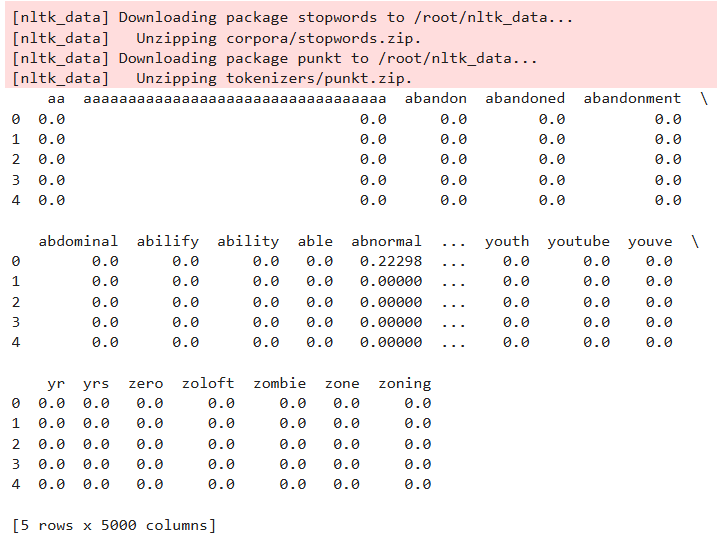
\includegraphics[width=0.8\textwidth]{Images/Output Data Preprocessing.png}  
    \caption{Data Preprocessing}
    \label{Data Preprocessing}  % Label for referencing the figure
\end{figure}

% Bag Of Words Model
\subsubsection{Implementation of Bag Of Words}

\noindent
The following code snippet implements the Bag of Words (BoW) model for the preprocessed dataset related to mental health. This process converts text data into a numerical format that can be used for machine learning tasks.

\begin{verbatim}
import pandas as pd
from sklearn.feature_extraction.text import CountVectorizer
# Load the preprocessed dataset
dataset = pd.read_csv('preprocessed_mental_health_text.csv')
# Check if 'cleaned_text' column exists
if 'cleaned_text' not in dataset.columns:
    raise ValueError("The dataset must have a 'cleaned_text' column. 
    Ensure text preprocessing has been done.")
# Remove rows with missing values in 'cleaned_text' column
dataset.dropna(subset=['cleaned_text'], inplace=True)
# Initialize the CountVectorizer
vectorizer = CountVectorizer()
# Fit and transform the cleaned text data
X = vectorizer.fit_transform(dataset['cleaned_text'])
# Convert the result to a DataFrame for better visualization (optional)
X_df = pd.DataFrame(X.toarray(), columns=vectorizer.
get_feature_names_out())
# Print the shape of the resulting matrix
print(f'Shape of Bag of Words matrix: {X_df.shape}')
# Print the first few rows of the Bag of Words DataFrame (optional)
print(X_df.head())
\end{verbatim}

\noindent
The code begins by importing the necessary libraries: \texttt{pandas} for data manipulation and \texttt{CountVectorizer} from \texttt{sklearn} for creating the Bag of Words model. It then loads a preprocessed dataset from a CSV file named \texttt{preprocessed\_mental\_health\_text.csv}. A check is performed to ensure that the dataset contains a column labeled \texttt{cleaned\_text}. If this column is absent, a \texttt{ValueError} is raised, prompting the user to ensure text preprocessing is completed. Following this, any rows with missing values in the \texttt{cleaned\_text} column are removed to maintain data integrity. Next, an instance of \texttt{CountVectorizer} is initialized, which will convert the cleaned text into a matrix of token counts. The \texttt{fit\_transform()} method is called on the cleaned text data, generating a sparse matrix \(X\) that represents the Bag of Words model. This matrix is then converted into a DataFrame \texttt{X\_df} for easier visualization, with columns corresponding to the unique words identified in the text. Finally, the shape of the resulting Bag of Words matrix is printed to the console, along with the first few rows of the DataFrame to provide a preview of the transformed data.

\begin{figure}[h!]  
    \centering
    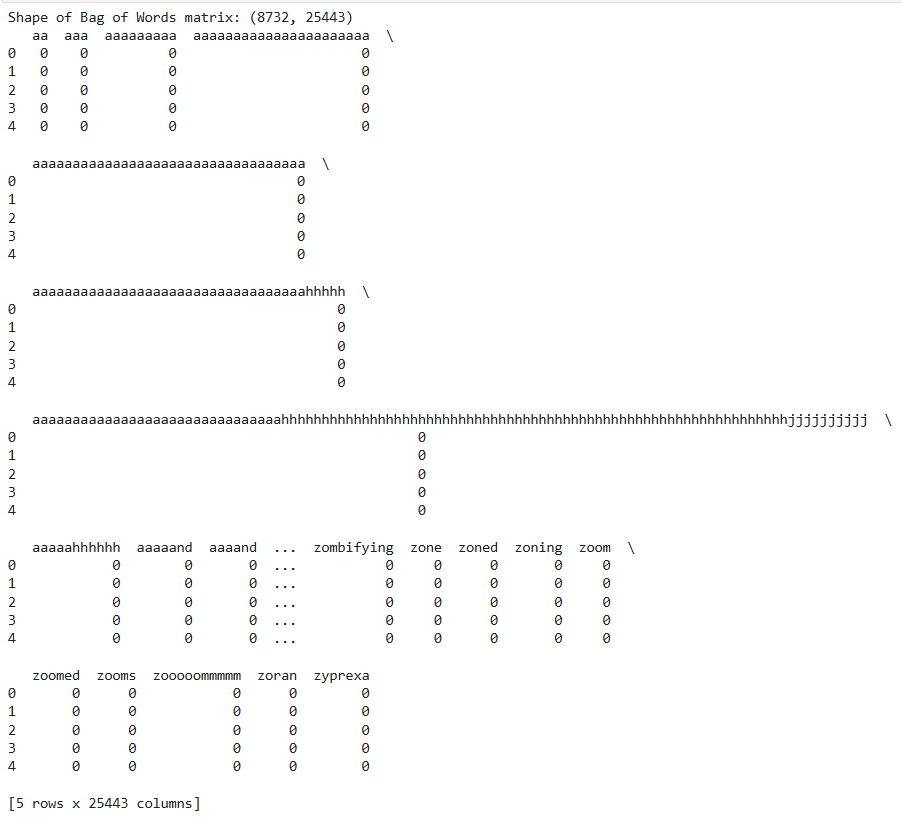
\includegraphics[width=0.8\textwidth]{Images/Output BOW.png}  
    \caption{Implementation of Bag Of Words}
    \label{BOW}  % Label for referencing the figure
\end{figure}

% Splitting DataSet
\subsubsection{Splitting Preprocessed Dataset}
\noindent
The following code snippet demonstrates how to split the preprocessed dataset into training and test sets, which is a crucial step in preparing data for machine learning models.

\begin{verbatim}
import pandas as pd
from sklearn.model_selection import train_test_split

# Load the preprocessed dataset
dataset = pd.read_csv('preprocessed_mental_health_text.csv')

# Check if 'cleaned_text' and 'mental_health_issue' columns exist
if 'cleaned_text' not in dataset.columns or 'mental_health_issue' 
not in dataset.columns:
    raise ValueError("The dataset must have 'cleaned_text' and 
    'mental_health_issue' columns.")

# Remove rows with missing values in 'cleaned_text' column
dataset.dropna(subset=['cleaned_text'], inplace=True) 
#This line has been added

# Initialize the CountVectorizer and fit/transform the cleaned text
from sklearn.feature_extraction.text import CountVectorizer

vectorizer = CountVectorizer()
X = vectorizer.fit_transform(dataset['cleaned_text'])

# Prepare the target variable
y = dataset['mental_health_issue']

# Split the dataset into Training and Test Sets
X_train, X_test, y_train, y_test = train_test_split(X, y, 
test_size=0.2, random_state=42)

# Print the shapes of the resulting datasets
print(f'Shape of X_train: {X_train.shape}')
print(f'Shape of X_test: {X_test.shape}')
print(f'Shape of y_train: {y_train.shape}')
print(f'Shape of y_test: {y_test.shape}')
\end{verbatim}

\noindent
The code begins by importing the necessary libraries, specifically \texttt{pandas} for data manipulation and \texttt{train\_test\_split} from \texttt{sklearn.model\_selection} for splitting the dataset. It then loads 
the preprocessed dataset from a CSV file named \newline
\texttt{preprocessed\_mental\_health\_text.csv}. A validation check is performed to ensure that both the \texttt{cleaned\_text} and 
\texttt{mental\_health\_issue} columns exist in the dataset; if not, a \texttt{ValueError} is raised to alert the user. Next, rows with missing values in the \texttt{cleaned\_text} column are removed to maintain data integrity. After this, the \texttt{CountVectorizer} is initialized to transform the cleaned text into a numerical format suitable for machine learning. The transformed text data is stored in the variable \(X\), while the target variable representing mental health issues is stored in \(y\). The dataset is then split into training and test sets, with 80\% of the data used for training and 20\% for testing, controlled by the \texttt{random\_state} parameter to ensure reproducibility. Finally, the shapes of the resulting training and test datasets are printed to the console, providing insights into the number of samples allocated for training and testing, which is essential for understanding the data distribution.

\begin{figure}[h!]  
    \centering
    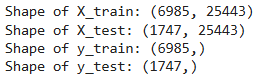
\includegraphics[width=0.6\textwidth]{Images/Output Splitting Dataset.png}  
    \caption{Splitting Dataset}
    \label{Splitting Dataset}  % Label for referencing the figure
\end{figure}


\subsubsection{Logistic Regression}
\noindent
The following code snippet demonstrates the training and evaluation of a Logistic Regression model using a preprocessed dataset related to mental health.

\begin{figure}[h!]  
    \centering
    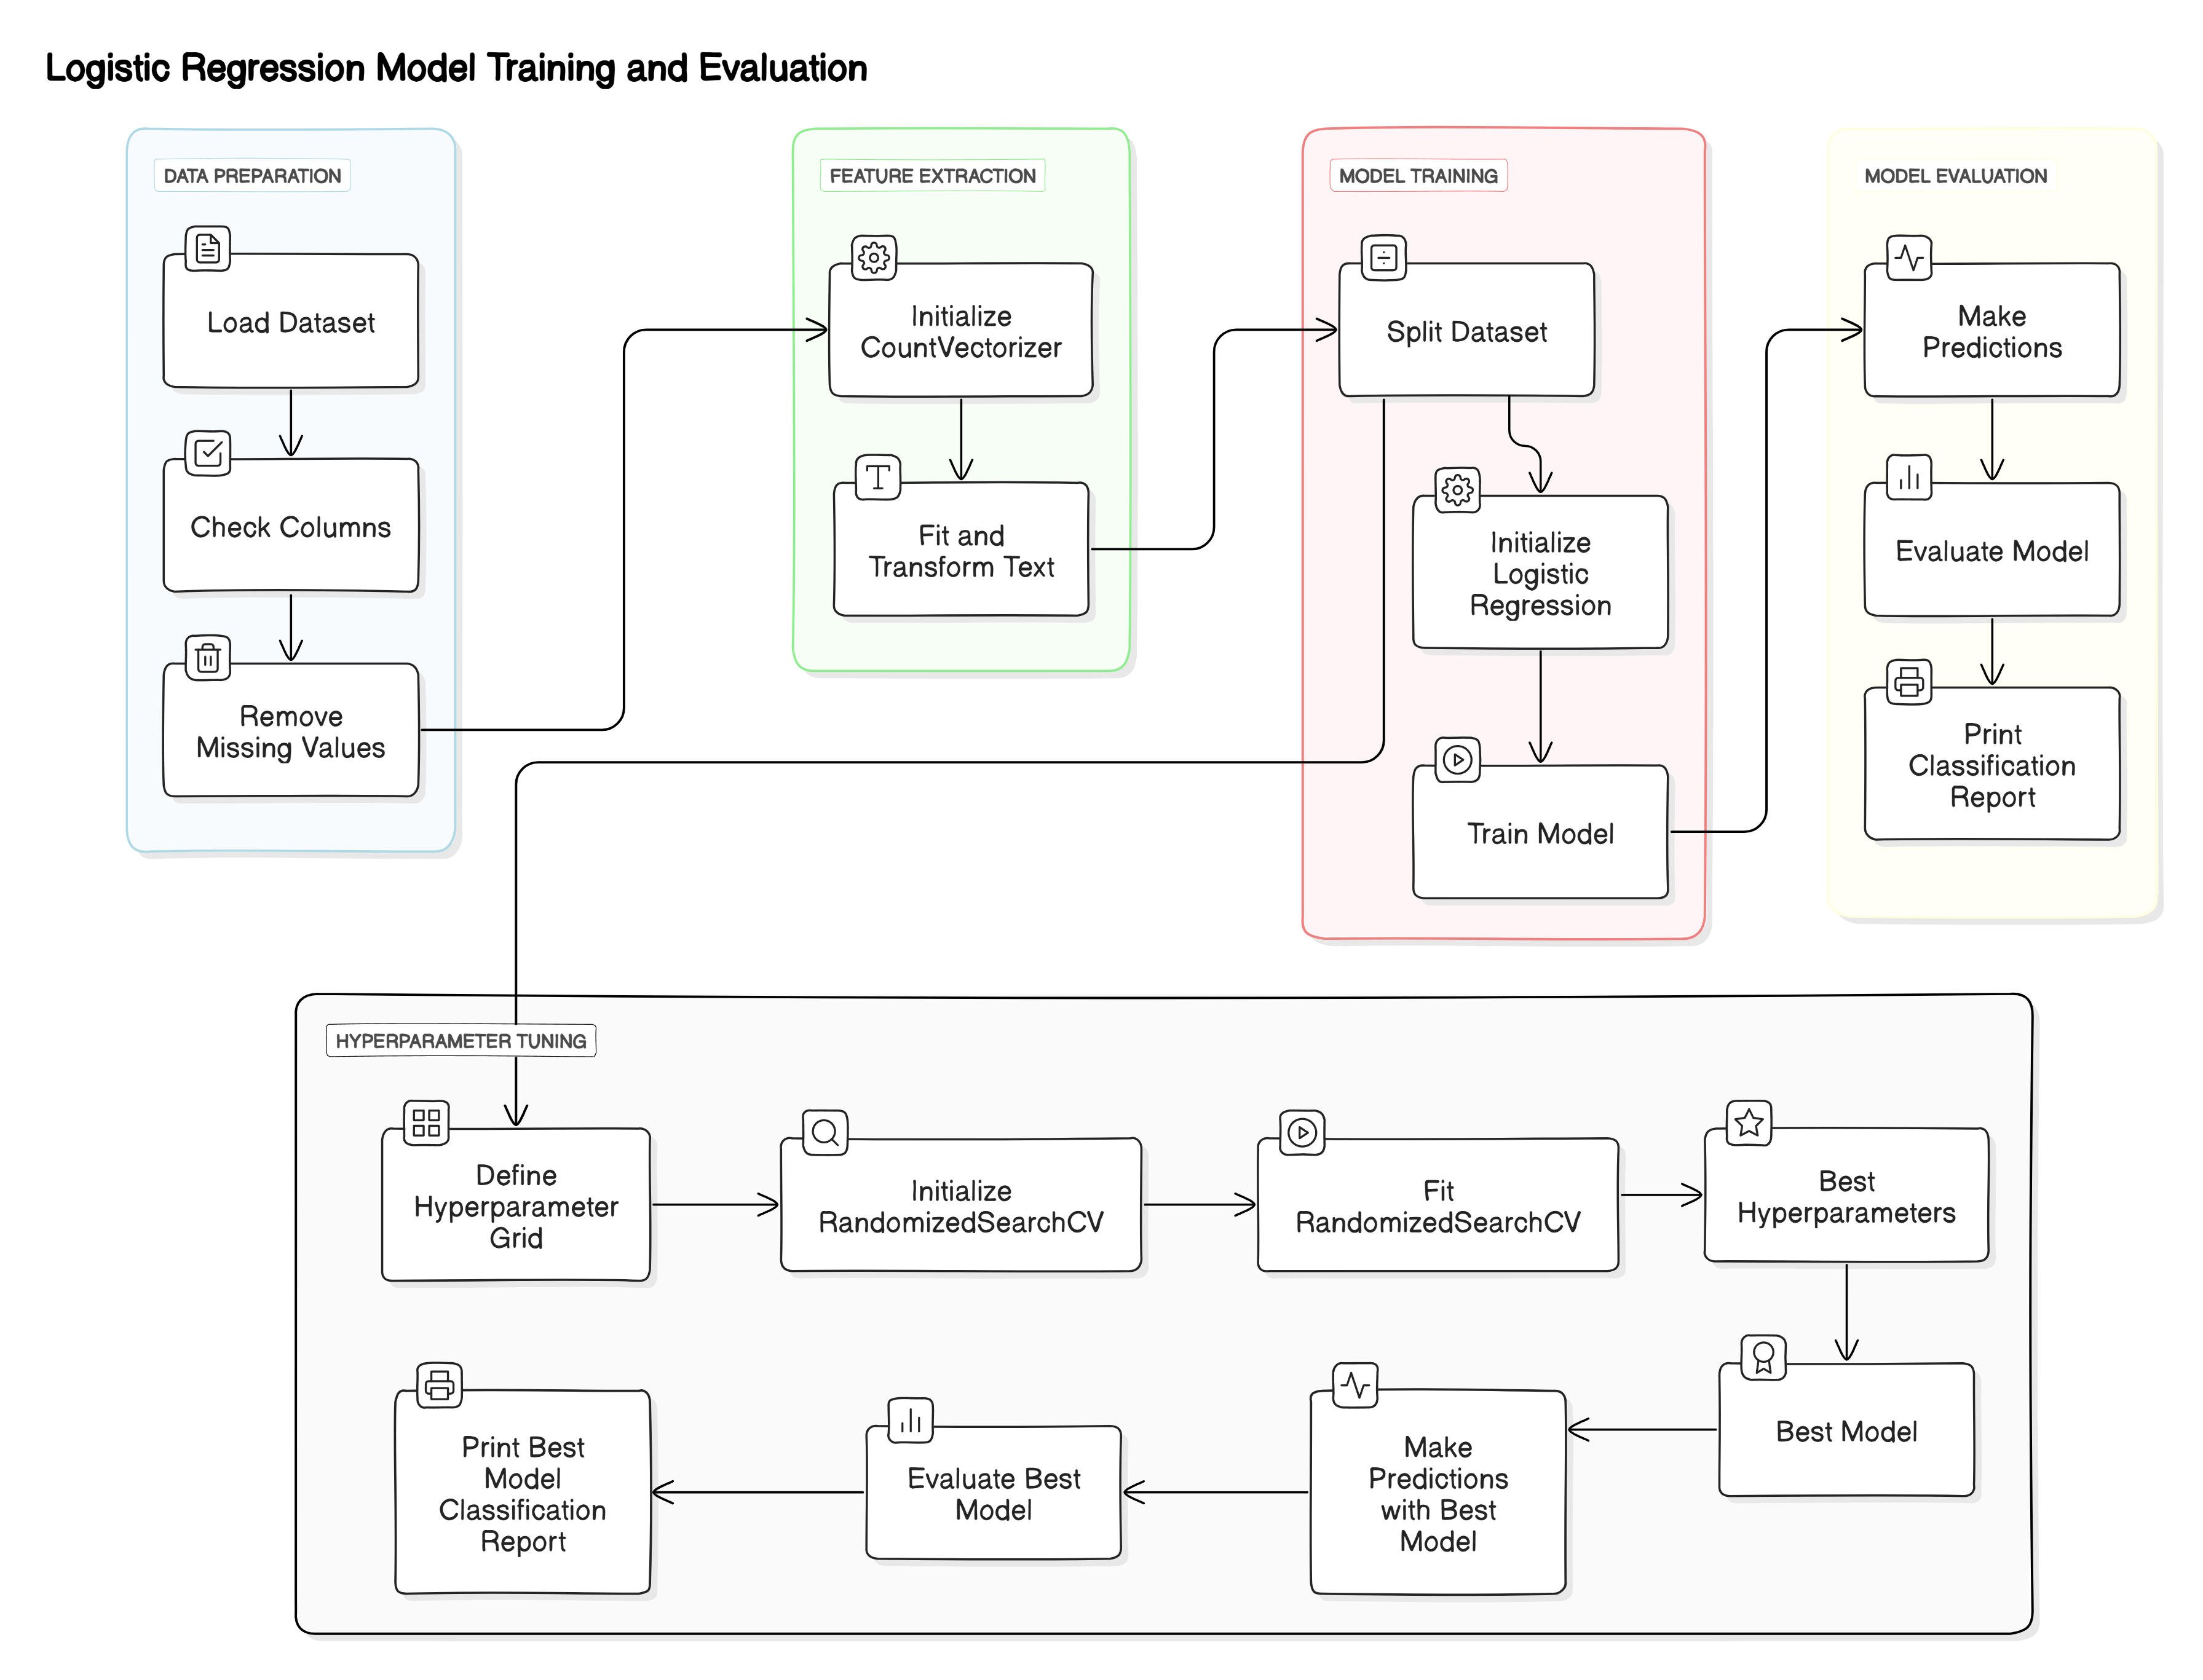
\includegraphics[width=1.0\textwidth]{Images/Logistic Regression.png}  
    \caption{Logistic Regression}
    \label{Logistic Regression}  % Label for referencing the figure
\end{figure}

\begin{verbatim}
import pandas as pd
from sklearn.model_selection import train_test_split
from sklearn.feature_extraction.text import CountVectorizer
from sklearn.linear_model import LogisticRegression
from sklearn.metrics import accuracy_score, classification_report
dataset = pd.read_csv('preprocessed_mental_health_text.csv')
if 'cleaned_text' not in dataset.columns or 'mental_health_issue' 
not in dataset.columns:
    raise ValueError("The dataset must have 'cleaned_text' and 
    'mental_health_issue' columns.")
dataset.dropna(subset=['cleaned_text'], inplace=True)
vectorizer = CountVectorizer()
X = vectorizer.fit_transform(dataset['cleaned_text'])
y = dataset['mental_health_issue']
X_train, X_test, y_train, y_test = train_test_split(X, y, 
test_size=0.2, random_state=42)
model = LogisticRegression(max_iter=2000)
model.fit(X_train, y_train)
y_pred = model.predict(X_test)
accuracy = accuracy_score(y_test, y_pred)
print(f'Accuracy: {accuracy * 100:.2f}%')
print("Classification Report:\n", classification_report(y_test, 
y_pred))
\end{verbatim}

\noindent
The code begins by importing necessary libraries, including \texttt{pandas} for data manipulation and various functions from \texttt{sklearn} for model training and evaluation. It then loads the preprocessed dataset from a CSV file named \texttt{preprocessed\_mental\_health\_text.csv}. A validation check ensures that the dataset contains the required columns, raising an error if either \texttt{cleaned\_text} or \texttt{mental\_health\_issue} is missing. Rows with missing values in the \texttt{cleaned\_text} column are removed to maintain data quality. The \texttt{CountVectorizer} is initialized and used to convert the cleaned text data into a matrix of token counts, stored in \(X\). The target variable, representing mental health issues, is assigned to \(y\). The dataset is then split into training and testing sets, with 80\% used for training and 20\% for testing. A Logistic Regression model is initialized and trained on the training data. Predictions are made on the test set, and the model's accuracy is calculated and printed. Finally, a classification report is generated, providing detailed metrics on the model’s performance across different categories.

\begin{figure}[h!]  
    \centering
    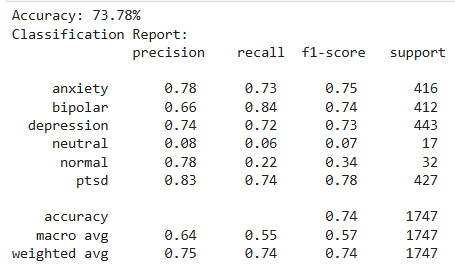
\includegraphics[width=0.8\textwidth]{Images/Output Logistic Regression.png}  
    \caption{Logistic Regression Result}
    \label{Logistic Regression Result}  % Label for referencing the figure
\end{figure}

\subsubsection{Hyperparameter Tuning on Logistic Regression using Random Search}

The following code snippet demonstrates how to perform hyperparameter tuning on a Logistic Regression model using Random Search.

\begin{verbatim}
import pandas as pd
from sklearn.model_selection import train_test_split, 
RandomizedSearchCV
from sklearn.feature_extraction.text import CountVectorizer
from sklearn.linear_model import LogisticRegression
from sklearn.metrics import accuracy_score, classification_report
dataset = pd.read_csv('preprocessed_mental_health_text.csv')
if 'cleaned_text' not in dataset.columns or 'mental_health_issue' 
not in dataset.columns:
    raise ValueError("The dataset must have 'cleaned_text' and 
    'mental_health_issue' columns.")
dataset.dropna(subset=['cleaned_text'], inplace=True)
vectorizer = CountVectorizer()
X = vectorizer.fit_transform(dataset['cleaned_text'])
y = dataset['mental_health_issue']
X_train, X_test, y_train, y_test = train_test_split(X, y, 
test_size=0.2, random_state=42)
model = LogisticRegression(max_iter=200)
param_distributions = {
    'C': [0.001, 0.01, 0.1, 1, 10, 100],
    'penalty': ['l1', 'l2', 'elasticnet', 'none'],
    'solver': ['liblinear', 'saga']
}
random_search = RandomizedSearchCV(estimator=model, 
param_distributions=param_distributions,
n_iter=10, scoring='accuracy', cv=5, n_jobs=-1, random_state=42)
random_search.fit(X_train, y_train)
print("Best Hyperparameters:", random_search.best_params_)
best_model = random_search.best_estimator_
y_pred = best_model.predict(X_test)
accuracy = accuracy_score(y_test, y_pred)
print(f'Accuracy: {accuracy * 100:.2f}%')
print("Classification Report:\n", 
classification_report(y_test, y_pred))
\end{verbatim}

\noindent
The code begins by importing the necessary libraries, including \texttt{pandas} for data manipulation and various functions from \texttt{sklearn} for model training and evaluation. It loads the preprocessed dataset from a CSV file named \newline \texttt{preprocessed\_mental\_health\_text.csv} and checks for the required columns \texttt{cleaned\_text} and \texttt{mental\_health\_issue}. If these columns are not present, a \texttt{ValueError} is raised. The code then removes any rows with missing values in the \texttt{cleaned\_text} column. The \texttt{CountVectorizer} is initialized to convert the cleaned text into a numerical format, which is stored in \(X\), while the target variable representing mental health issues is stored in \(y\). The dataset is split into training and testing sets with 80\% for training and 20\% for testing. A Logistic Regression model is created with a maximum of 200 iterations. The hyperparameter grid for tuning is defined, specifying values for the inverse of regularization strength (\texttt{C}), types of regularization (\texttt{penalty}), and solvers. A \texttt{RandomizedSearchCV} object is initialized to perform the random search over the hyperparameter grid, and the model is fitted using the training data. The best hyperparameters are printed, and the best model is used to make predictions on the test set. Finally, the model's accuracy is calculated and displayed, along with a classification report that provides detailed metrics on the model's performance across different categories.

\begin{figure}[h!]  
    \centering
    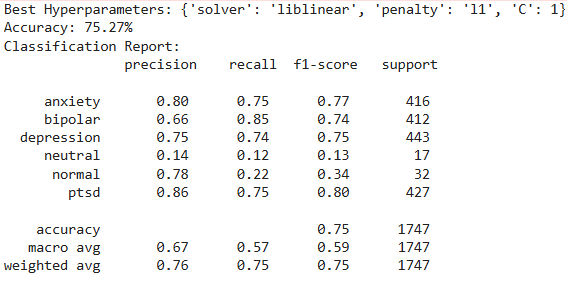
\includegraphics[width=0.6\textwidth]{Images/Output HPT LR.png}  
    \caption{Result of Hyperparameter Tuning on Logistic Regression}
    \label{Project Modules}  % Label for referencing the figure
\end{figure}

\begin{figure}[h!]  
    \centering
    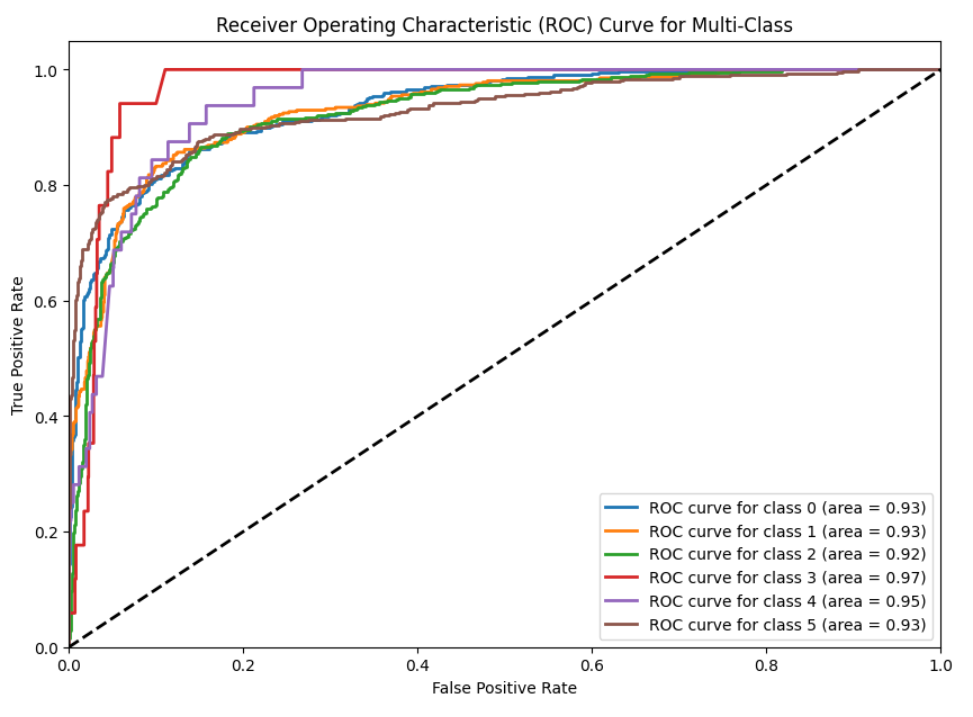
\includegraphics[width=0.6\textwidth]{Images/ROC LR.png}  
    \caption{ROC Curve on Logistic Regression}
    \label{ROC LR}  % Label for referencing the figure
\end{figure}


\subsubsection{K Nearest Neighbours}
\noindent
The following code snippet demonstrates the implementation of the k-Nearest Neighbors (k-NN) algorithm for classifying mental health issues based on preprocessed text data.

\begin{figure}[h!]  
    \centering
    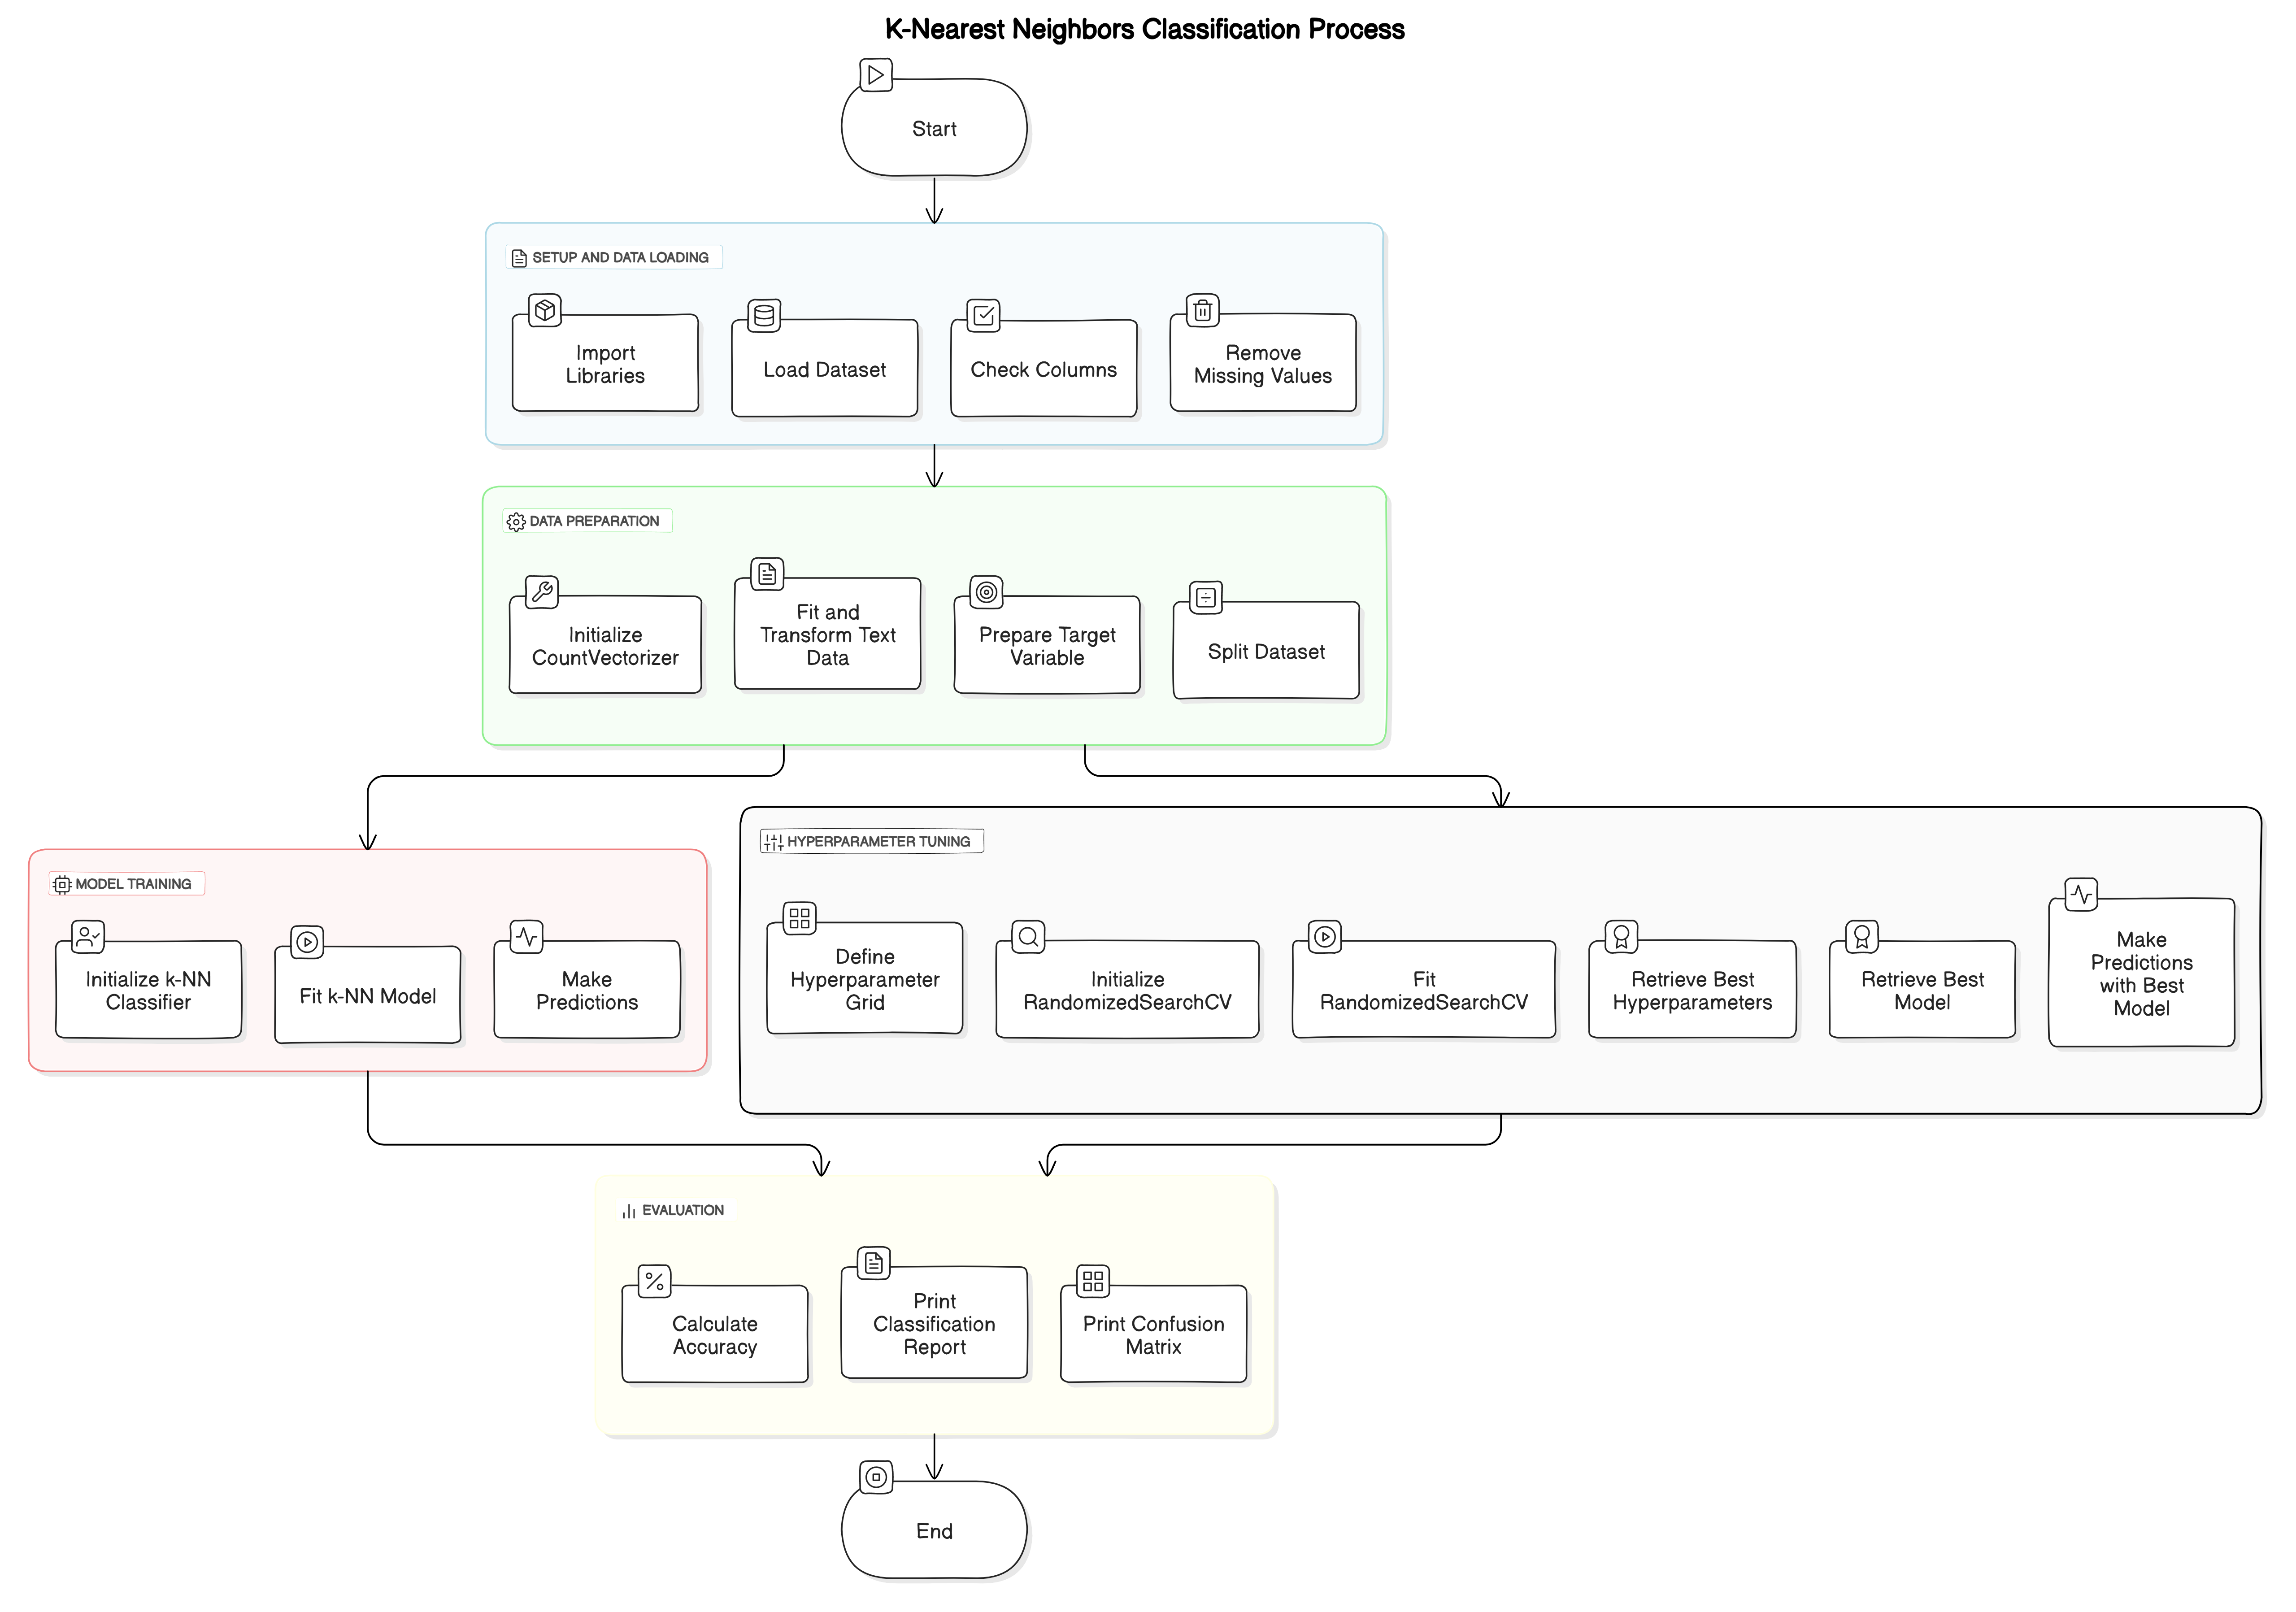
\includegraphics[width=1.0\textwidth]{Images/KNN.png}  
    \caption{K Nearest Neighbours Workflow}
    \label{KNN}  % Label for referencing the figure
\end{figure}


\begin{verbatim}
import pandas as pd
from sklearn.model_selection import train_test_split
from sklearn.feature_extraction.text import CountVectorizer
from sklearn.neighbors import KNeighborsClassifier
from sklearn.metrics import accuracy_score, classification_report, 
confusion_matrix
dataset = pd.read_csv('preprocessed_mental_health_text.csv')
if 'cleaned_text' not in dataset.columns or 'mental_health_issue' 
not in dataset.columns:
    raise ValueError("The dataset must have 'cleaned_text' and 
    'mental_health_issue' columns.")
dataset.dropna(subset=['cleaned_text'], inplace=True)
vectorizer = CountVectorizer()
X = vectorizer.fit_transform(dataset['cleaned_text'])
y = dataset['mental_health_issue']
X_train, X_test, y_train, y_test = train_test_split(X, y, 
test_size=0.2, random_state=42)
knn = KNeighborsClassifier(n_neighbors=5)
knn.fit(X_train, y_train)
y_pred = knn.predict(X_test)
accuracy = accuracy_score(y_test, y_pred)
print(f'Accuracy: {accuracy * 100:.2f}%')
print("Classification Report:\n", 
classification_report(y_test, y_pred))
print("Confusion Matrix:\n", confusion_matrix(y_test,y_pred))
\end{verbatim}

\noindent
The code begins by importing the necessary libraries, including \texttt{pandas} for data manipulation, \texttt{train\_test\_split} for splitting the dataset, \texttt{CountVectorizer} for transforming text data, and \texttt{KNeighborsClassifier} along with various metrics from \texttt{sklearn} for model evaluation. It loads the preprocessed dataset from a CSV file named \newline
\texttt{preprocessed\_mental\_health\_text.csv} and checks that both the \texttt{cleaned\_text} and \texttt{mental\_health\_issue} columns are present; if not, a \texttt{ValueError} is raised. Rows with missing values in the \texttt{cleaned\_text} column are removed to maintain data integrity. The \texttt{CountVectorizer} is initialized to convert the cleaned text into a numerical format, stored in \(X\), while the target variable representing mental health issues is assigned to \(y\). The dataset is split into training and testing sets, with 80\% used for training and 20\% for testing. A k-NN classifier is initialized with 5 neighbors, and the model is fitted on the training data. Predictions are made on the test set, and the model's accuracy is calculated and displayed. Finally, a classification report and confusion matrix are printed, providing detailed metrics on the model's performance and insight into its classification results.

\begin{figure}[h!]  
    \centering
    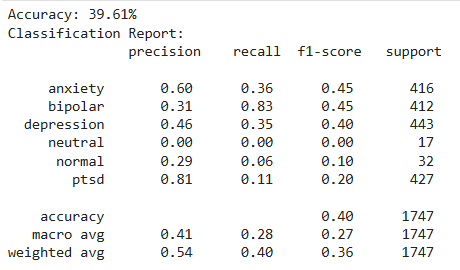
\includegraphics[width=0.6\textwidth]{Images/Output KNN.png}  
    \caption{K Nearest Neighbours Result}
    \label{KNN}  % Label for referencing the figure
\end{figure}

\subsubsection{Hyperparameter Tuning on KNN Using Random Search}
\noindent
The following code snippet demonstrates how to perform hyperparameter tuning on a k-Nearest Neighbors (k-NN) classifier using Random Search to optimize its performance.

\begin{verbatim}
import pandas as pd
from sklearn.model_selection import train_test_split, 
RandomizedSearchCV
from sklearn.feature_extraction.text import CountVectorizer
from sklearn.neighbors import KNeighborsClassifier
from sklearn.metrics import accuracy_score, classification_report, 
confusion_matrix
dataset = pd.read_csv('preprocessed_mental_health_text.csv')
if 'cleaned_text' 
not in dataset.columns or 'mental_health_issue' not in dataset.columns:
    raise ValueError("The dataset must have 'cleaned_text' and 
    'mental_health_issue' columns.")
dataset.dropna(subset=['cleaned_text'], inplace=True)
vectorizer = CountVectorizer()
X = vectorizer.fit_transform(dataset['cleaned_text'])
y = dataset['mental_health_issue']
X_train, X_test, y_train, y_test = train_test_split(X, y, 
test_size=0.2, random_state=42)
knn = KNeighborsClassifier()
param_distributions = {
    'n_neighbors': [3, 4, 5, 6, 7, 8, 9, 10, 11, 12, 13, 
    14, 15, 16, 17, 18, 19, 20],
    'metric': ['euclidean', 'manhattan', 'chebyshev', 'minkowski'],
    'weights': ['uniform', 'distance']
}
random_search = RandomizedSearchCV(estimator=knn, 
param_distributions=param_distributions, 
n_iter=200, scoring='accuracy', cv=5, n_jobs=-1, random_state=42)
random_search.fit(X_train, y_train)
print("Best Hyperparameters:", random_search.best_params_)
best_knn = random_search.best_estimator_
y_pred = best_knn.predict(X_test)
accuracy = accuracy_score(y_test, y_pred)
print(f'Accuracy: {accuracy * 100:.2f}%')
print("Classification Report:\n", 
classification_report(y_test, y_pred))
print("Confusion Matrix:\n", confusion_matrix(y_test, y_pred))
\end{verbatim}

\noindent
The code starts by importing the required libraries, including \texttt{pandas} for data manipulation, and various functions from \texttt{sklearn} for model training, evaluation, and hyperparameter tuning. It loads the preprocessed dataset from a CSV file named \newline \texttt{preprocessed\_mental\_health\_text.csv} and checks for the presence of the necessary columns, raising a \texttt{ValueError} if they are missing. Rows with missing values in the \texttt{cleaned\_text} column are removed to ensure data quality. The \texttt{CountVectorizer} is initialized to convert the cleaned text into a numerical format, stored in \(X\), while the target variable representing mental health issues is assigned to \(y\). The dataset is split into training and testing sets, with 80\% used for training and 20\% for testing. A k-NN classifier is initialized, and a hyperparameter grid is defined, specifying different values for the number of neighbors, distance metrics, and weighting options for the neighbors. The \texttt{RandomizedSearchCV} object is created to perform random search over the hyperparameter grid, and the model is fitted using the training data. After fitting, the best hyperparameters are printed, along with the best k-NN model derived from the search. Predictions are made on the test set, and the accuracy of the model is calculated and displayed. Finally, a classification report and confusion matrix are printed to evaluate the model's performance and provide insights into its classification results.

\begin{figure}[h!]  
    \centering
    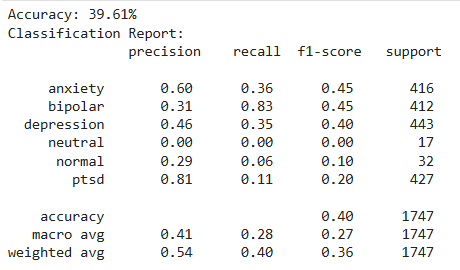
\includegraphics[width=0.8\textwidth]{Images/Output KNN.png}  
    \caption{Result of Hyperparameter Tuning on KNN}
    \label{HPT KNN}  % Label for referencing the figure
\end{figure}

\begin{figure}[h!]  
    \centering
    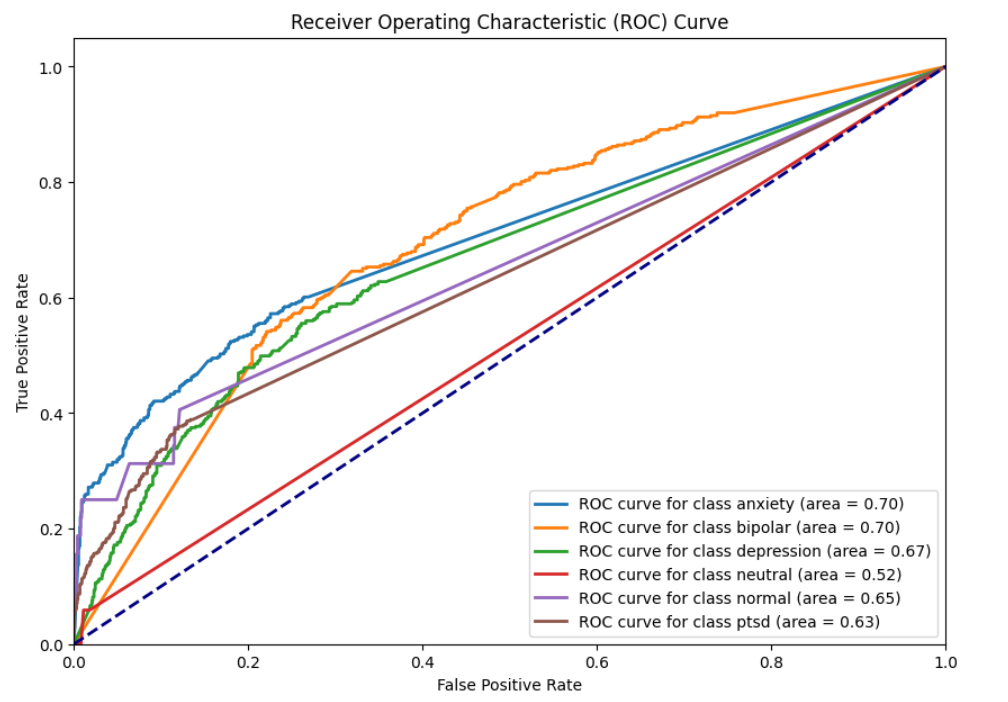
\includegraphics[width=0.8\textwidth]{Images/ROC KNN.png}  
    \caption{ROC curve on KNN}
    \label{ROC KNN}  % Label for referencing the figure
\end{figure}


\subsubsection{Support Vector Machine}
\noindent
The following code snippet demonstrates the implementation of a Support Vector Machine (SVM) classifier for classifying mental health issues based on preprocessed text data.

\begin{figure}[h!]  
    \centering
    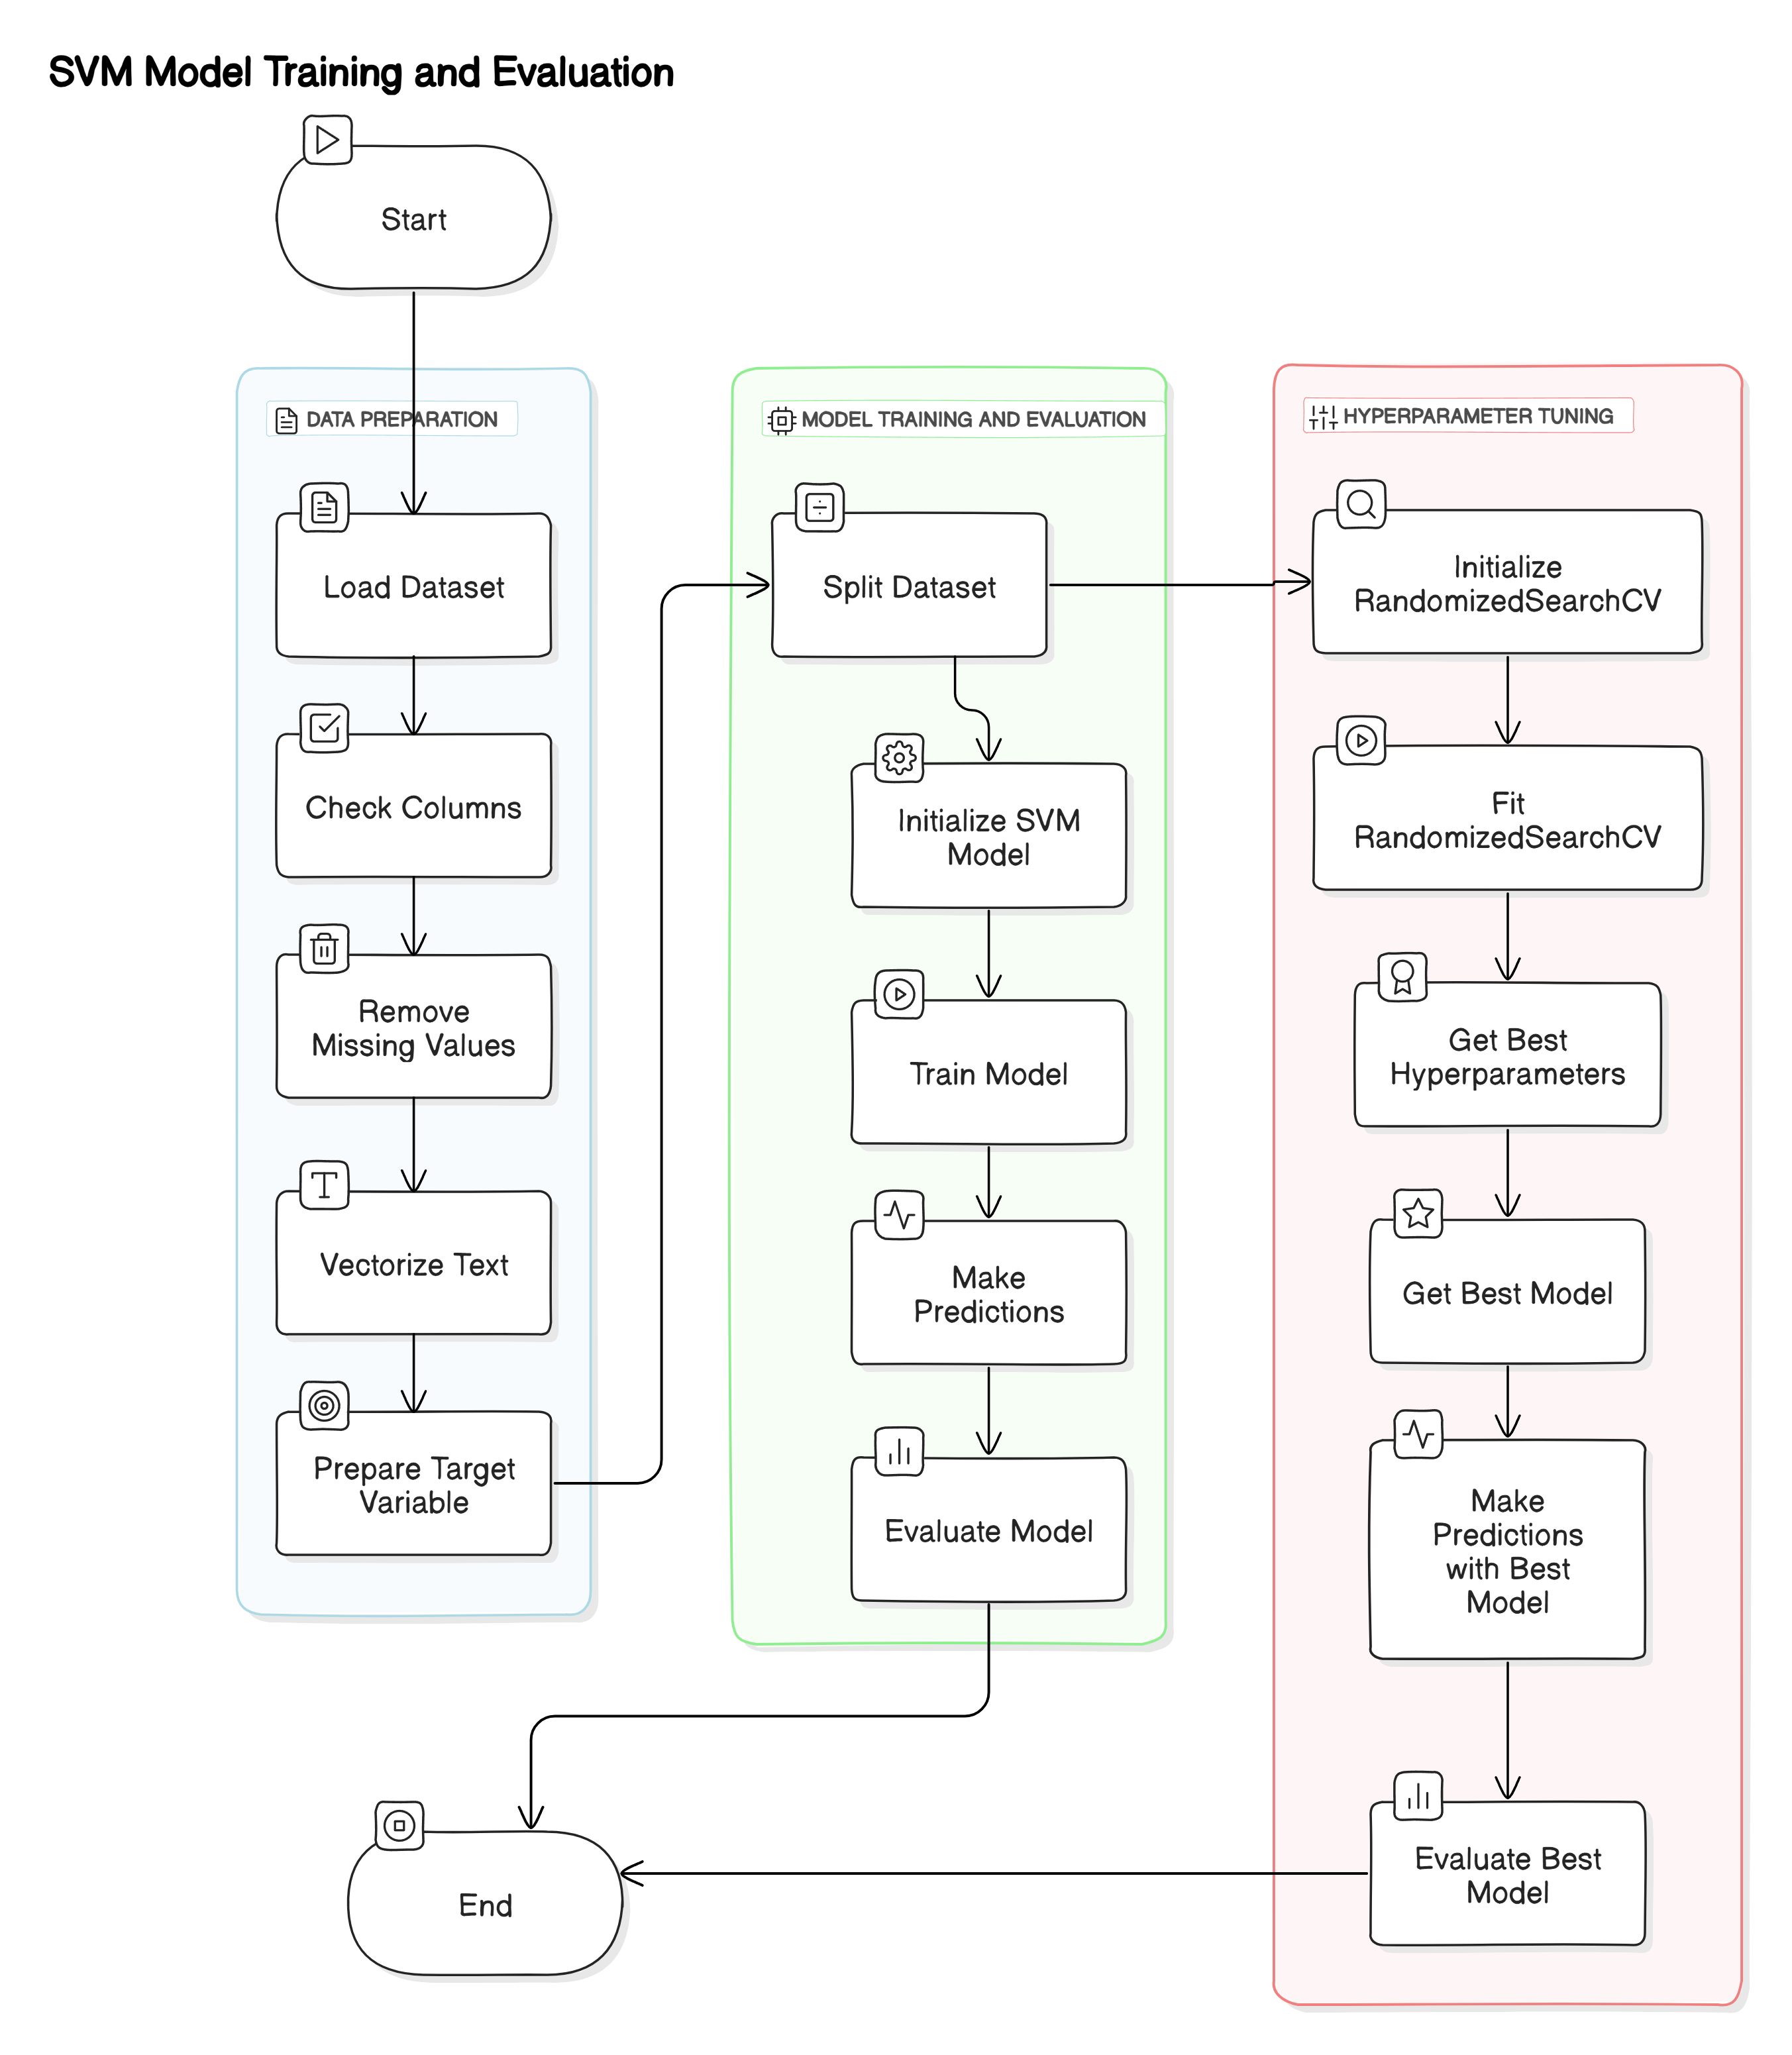
\includegraphics[width=0.6\textwidth]{Images/SVM.png}  
    \caption{Support Vector Machine Workflow}
    \label{SVM}  % Label for referencing the figure
\end{figure}

\begin{verbatim}
import pandas as pd
from sklearn.model_selection import train_test_split
from sklearn.feature_extraction.text import CountVectorizer
from sklearn.svm import SVC
from sklearn.metrics import accuracy_score, classification_report, 
confusion_matrix
dataset = pd.read_csv('preprocessed_mental_health_text.csv')
if 'cleaned_text' not in dataset.columns or 'mental_health_issue' 
not in dataset.columns:
    raise ValueError("The dataset must have 'cleaned_text' and 
    'mental_health_issue' columns.")
dataset.dropna(subset=['cleaned_text'], inplace=True)
vectorizer = CountVectorizer()
X = vectorizer.fit_transform(dataset['cleaned_text'])
y = dataset['mental_health_issue']
X_train, X_test, y_train, y_test = train_test_split(X, y, 
test_size=0.2, random_state=42)
svm_model = SVC(kernel='linear', C=1, random_state=42)
svm_model.fit(X_train, y_train)
y_pred = svm_model.predict(X_test)
accuracy = accuracy_score(y_test, y_pred)
print(f'Accuracy: {accuracy * 100:.2f}%')
print("Classification Report:\n", 
classification_report(y_test, y_pred))
print("Confusion Matrix:\n", confusion_matrix(y_test, y_pred))
\end{verbatim}

\noindent
The code begins by importing the necessary libraries, including \texttt{pandas} for data manipulation and various functions from \texttt{sklearn} for model training and evaluation. It loads the preprocessed dataset from a CSV file named \newline \texttt{preprocessed\_mental\_health\_text.csv} and verifies that both the \texttt{cleaned\_text} and \texttt{mental\_health\_issue} columns exist, raising a \texttt{ValueError} if they are missing. Rows with missing values in the \texttt{cleaned\_text} column are removed to maintain data quality. The \texttt{CountVectorizer} is initialized to convert the cleaned text into a numerical format, stored in \(X\), while the target variable representing mental health issues is assigned to \(y\). The dataset is then split into training and testing sets, with 80\% used for training and 20\% for testing. An SVM model is initialized with a linear kernel and a regularization parameter \(C\) set to 1, which can be adjusted based on the specific needs of the analysis. The model is trained using the training data, and predictions are made on the test set. The accuracy of the model is calculated and displayed, along with a classification report and confusion matrix, which provide insights into the model's performance across different categories and the distribution of classification results.

\begin{figure}[h!]  
    \centering
    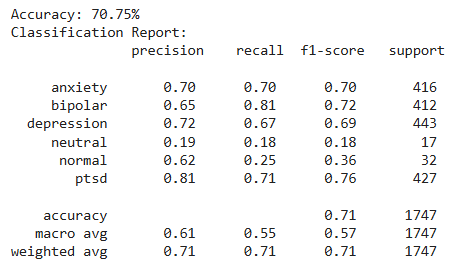
\includegraphics[width=0.6\textwidth]{Images/Output SVM.png}  
    \caption{Support Vector Machine (Linear Kernel) Result}
    \label{SVM}  % Label for referencing the figure
\end{figure}

\subsubsection{Hyperparameter Tuning on SVM using Random Search}
\noindent
The following code snippet demonstrates how to perform hyperparameter tuning on a Support Vector Machine (SVM) classifier using Random Search to optimize its performance.

\begin{verbatim}
import pandas as pd
from sklearn.model_selection import train_test_split, 
RandomizedSearchCV
from sklearn.feature_extraction.text import CountVectorizer
from sklearn.svm import SVC
from sklearn.metrics import accuracy_score, classification_report
dataset = pd.read_csv('preprocessed_mental_health_text.csv')
if 'cleaned_text' not in dataset.columns or 'mental_health_issue'
not in dataset.columns:
    raise ValueError("The dataset must have 'cleaned_text' and 
    'mental_health_issue' columns.")
dataset.dropna(subset=['cleaned_text'], inplace=True)
vectorizer = CountVectorizer()
X = vectorizer.fit_transform(dataset['cleaned_text'])
y = dataset['mental_health_issue']
X_train, X_test, y_train, y_test = train_test_split(X, y, 
test_size=0.2, random_state=42)
model = SVC()
param_distributions = {
    'C': [0.1, 1, 10, 100],
    'kernel': ['linear', 'rbf', 'poly'],
    'gamma': ['scale', 'auto', 0.1, 1],
}
random_search = RandomizedSearchCV(estimator=model, 
param_distributions=param_distributions, 
n_iter=200, scoring='accuracy', 
cv=5, n_jobs=-1, random_state=42)
random_search.fit(X_train, y_train)
print("Best Hyperparameters:", random_search.best_params_)
best_model = random_search.best_estimator_
y_pred = best_model.predict(X_test)
accuracy = accuracy_score(y_test, y_pred)
print(f'Accuracy: {accuracy * 100:.2f}%')
print("Classification Report:\n", 
classification_report(y_test, y_pred))
\end{verbatim}

\noindent
The code begins by importing the required libraries, including \texttt{pandas} for data manipulation and various functions from \texttt{sklearn} for model training and evaluation. It loads the preprocessed dataset from a CSV file named \newline \texttt{preprocessed\_mental\_health\_text.csv} and checks for the necessary columns, raising a \texttt{ValueError} if either the \texttt{cleaned\_text} or \texttt{mental\_health\_issue} columns are missing. Rows with missing values in the \texttt{cleaned\_text} column are then removed to ensure data quality. The \texttt{CountVectorizer} is initialized to convert the cleaned text into a numerical format, stored in \(X\), while the target variable representing mental health issues is assigned to \(y\). The dataset is split into training and testing sets, with 80\% used for training and 20\% for testing. An SVM model is initialized, and a hyperparameter grid is defined that specifies different values for the regularization parameter \(C\), various kernel types, and kernel coefficients. The \texttt{RandomizedSearchCV} object is created to perform random search over the hyperparameter grid, and the model is fitted using the training data. After fitting, the best hyperparameters are printed along with the best SVM model derived from the search. Predictions are made on the test set, and the accuracy of the model is calculated and displayed, along with a classification report that provides detailed metrics on the model's performance.

\begin{figure}[h!]  
    \centering
    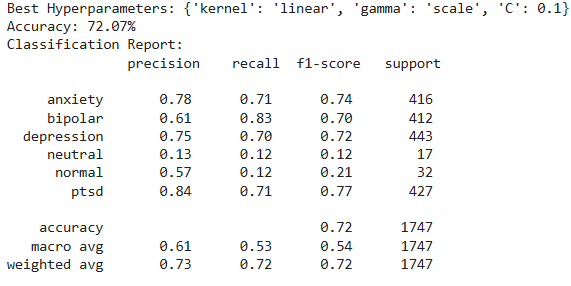
\includegraphics[width=0.8\textwidth]{Images/Output HPT SVM.png}  
    \caption{Result of Hyperparameter Tuning on SVM}
    \label{HPT SVM}  % Label for referencing the figure
\end{figure}

\begin{figure}[h!]  
    \centering
    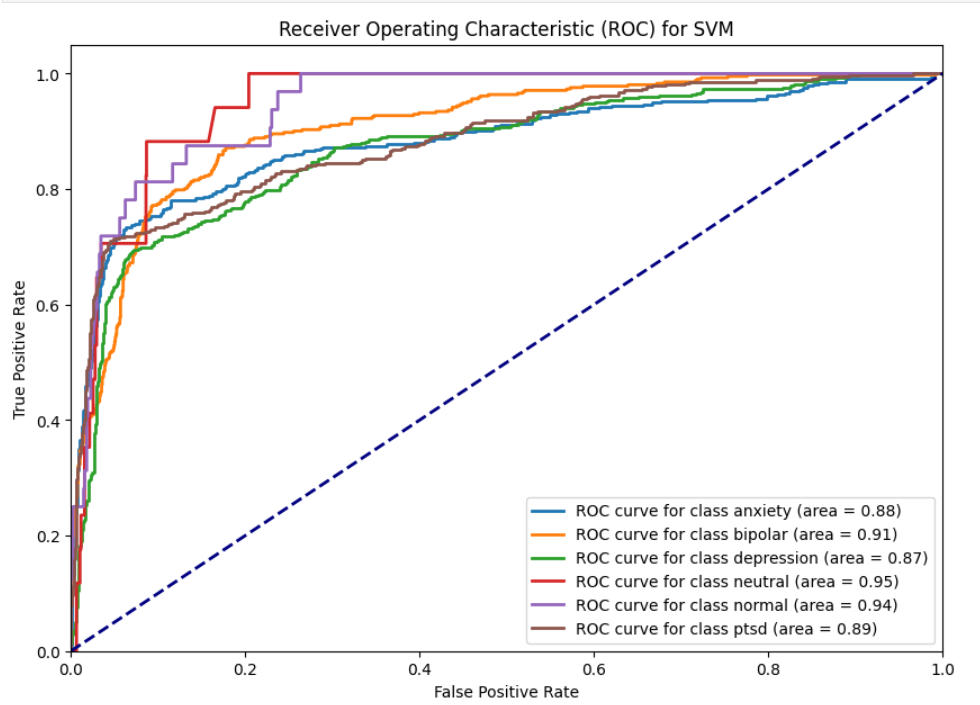
\includegraphics[width=0.8\textwidth]{Images/ROC SVM.png}  
    \caption{ROC Curve on SVM}
    \label{ROC SVM}  % Label for referencing the figure
\end{figure}

\pagebreak

\subsubsection{Naive Bayes Result}
\noindent
The following code snippet demonstrates the implementation of a Naive Bayes classifier for classifying mental health issues based on preprocessed text data.

\begin{figure}[h!]  
    \centering
    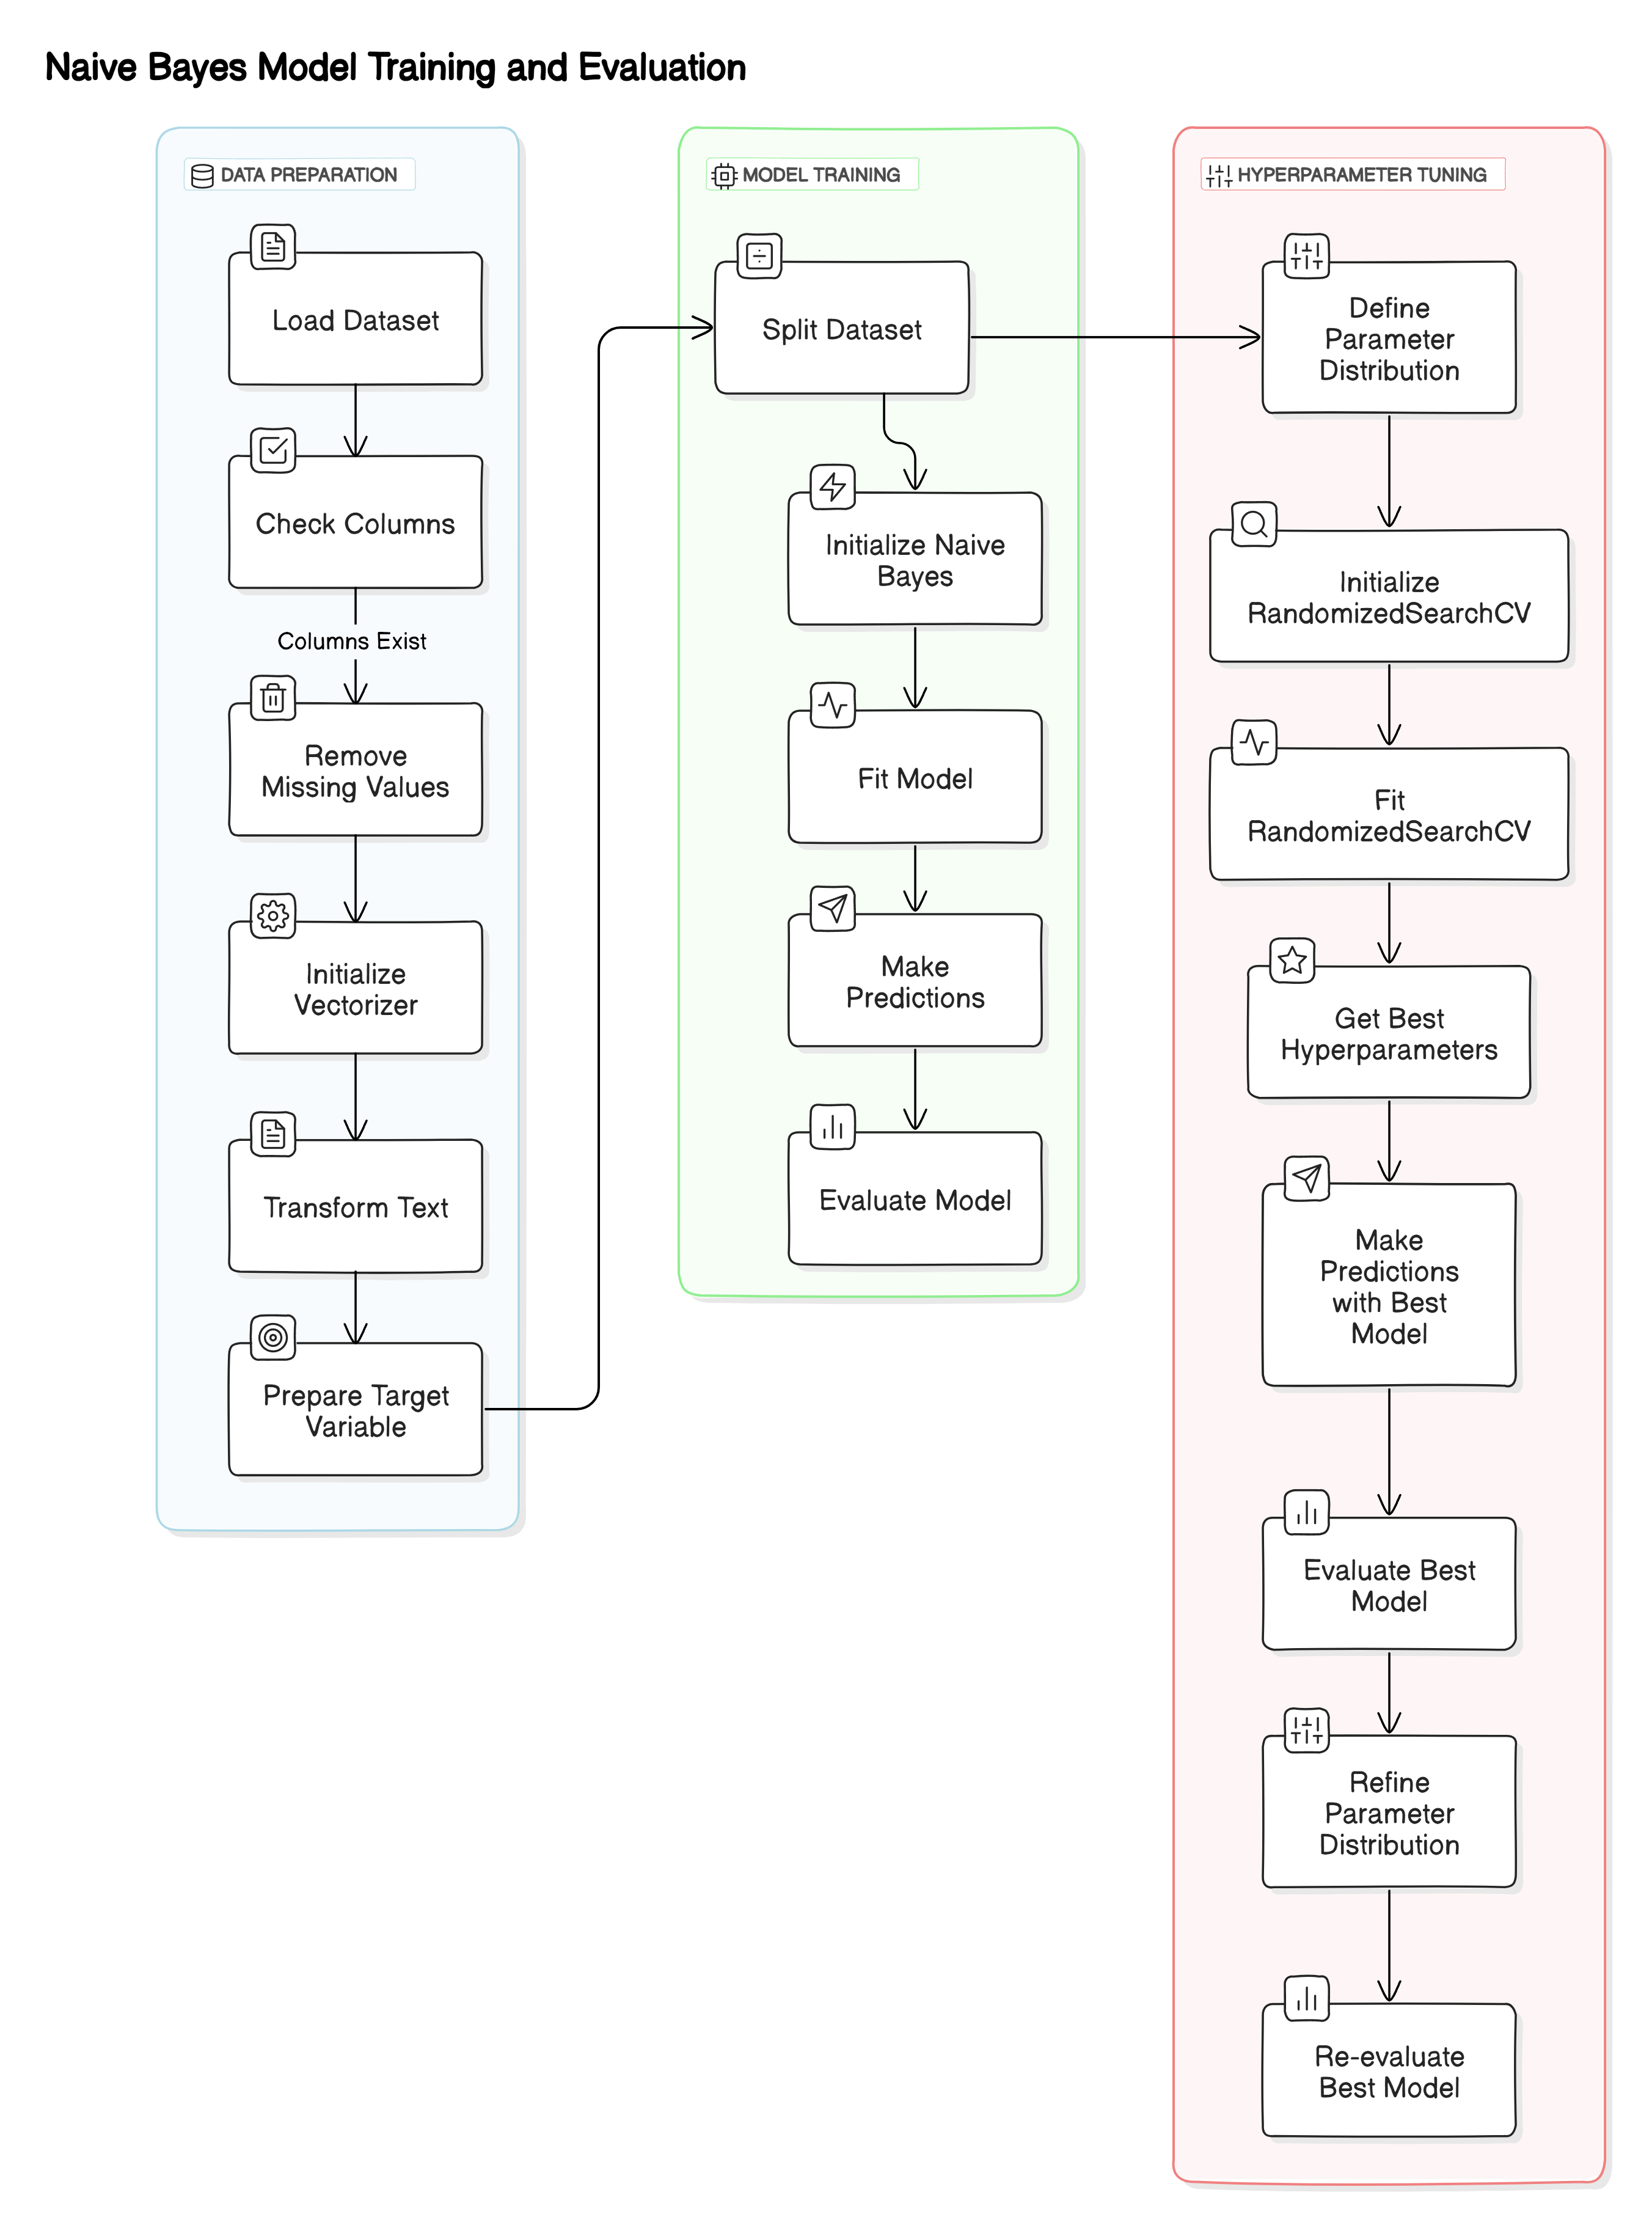
\includegraphics[width=1.0\textwidth]{Images/Naive Bayes.png}  
    \caption{Naive Bayes Workflow}
    \label{Naive Bayes}  % Label for referencing the figure
\end{figure}

\begin{verbatim}
import pandas as pd
from sklearn.model_selection import train_test_split
from sklearn.feature_extraction.text import CountVectorizer
from sklearn.naive_bayes import MultinomialNB
from sklearn.metrics import accuracy_score, classification_report, 
confusion_matrix
dataset = pd.read_csv('preprocessed_mental_health_text.csv')
if 'cleaned_text' not in dataset.columns or 'mental_health_issue' 
not in dataset.columns:
    raise ValueError("The dataset must have 'cleaned_text' and 
    'mental_health_issue' columns.")
dataset.dropna(subset=['cleaned_text'], inplace=True)
vectorizer = CountVectorizer()
X = vectorizer.fit_transform(dataset['cleaned_text'])
y = dataset['mental_health_issue']
X_train, X_test, y_train, y_test = train_test_split(X, y, 
test_size=0.2, random_state=42)
naive_bayes_model = MultinomialNB()
naive_bayes_model.fit(X_train, y_train)
y_pred = naive_bayes_model.predict(X_test)
accuracy = accuracy_score(y_test, y_pred)
print(f'Accuracy: {accuracy * 100:.2f}%')
print("Classification Report:\n", 
classification_report(y_test, y_pred))
print("Confusion Matrix:\n", confusion_matrix(y_test, y_pred))
\end{verbatim}

\noindent
The code begins by importing the necessary libraries, including \texttt{pandas} for data manipulation and various functions from \texttt{sklearn} for model training and evaluation. It loads the preprocessed dataset from a CSV file named \newline
\texttt{preprocessed\_mental\_health\_text.csv} and checks for the required columns, raising a \texttt{ValueError} if either the \texttt{cleaned\_text} or \texttt{mental\_health\_issue} columns are missing. Rows with missing values in the \texttt{cleaned\_text} column are then removed to ensure data quality. The \texttt{CountVectorizer} is initialized to convert the cleaned text into a numerical format, which is stored in \(X\), while the target variable representing mental health issues is assigned to \(y\). The dataset is split into training and testing sets, with 80\% used for training and 20\% for testing. A Naive Bayes classifier, specifically \texttt{MultinomialNB}, is initialized and fitted using the training data. Predictions are made on the test set, and the model's accuracy is calculated and displayed. Finally, a classification report and confusion matrix are printed, providing detailed metrics on the model's performance across different categories and insights into its classification results.

\begin{figure}[h!]  
    \centering
    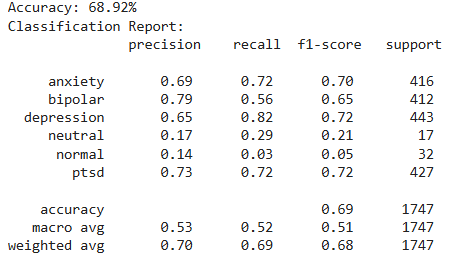
\includegraphics[width=0.8\textwidth]{Images/Output NB.png}  
    \caption{Naive Bayes}
    \label{NB}  % Label for referencing the figure
\end{figure}

\subsubsection{Hyperparameter Tuning on Naive Bayes using Random Search}
\noindent
The following code snippet demonstrates how to perform hyperparameter tuning on a Naive Bayes classifier using Random Search to optimize its performance.

\begin{verbatim}
import pandas as pd
from sklearn.model_selection import train_test_split, 
RandomizedSearchCV
from sklearn.feature_extraction.text import CountVectorizer
from sklearn.naive_bayes import MultinomialNB
from sklearn.metrics import accuracy_score, classification_report, 
confusion_matrix
from scipy.stats import uniform
dataset = pd.read_csv('preprocessed_mental_health_text.csv')
if 'cleaned_text' not in dataset.columns or 'mental_health_issue' 
not in dataset.columns:
    raise ValueError("The dataset must have 'cleaned_text' and 
    'mental_health_issue' columns.")
dataset.dropna(subset=['cleaned_text'], inplace=True)
vectorizer = CountVectorizer()
X = vectorizer.fit_transform(dataset['cleaned_text'])
y = dataset['mental_health_issue']
X_train, X_test, y_train, y_test = train_test_split(X, y, 
test_size=0.2, random_state=42)
naive_bayes_model = MultinomialNB()
param_distributions = {
    'alpha': uniform(0.001, 5.0)
}
random_search = RandomizedSearchCV(estimator=naive_bayes_model, 
param_distributions=param_distributions, n_iter=2000, 
scoring='accuracy', cv=5, n_jobs=-1, random_state=42)
random_search.fit(X_train, y_train)
print("Best Hyperparameters:", random_search.best_params_)
best_model = random_search.best_estimator_
y_pred = best_model.predict(X_test)
accuracy = accuracy_score(y_test, y_pred)
print(f'Accuracy: {accuracy * 100:.2f}%')
print("Classification Report:\n", 
classification_report(y_test, y_pred))
print("Confusion Matrix:\n", confusion_matrix(y_test, y_pred))
\end{verbatim}

\noindent
The code begins by importing the necessary libraries, including \texttt{pandas} for data manipulation, various functions from \texttt{sklearn} for model training and evaluation, and \texttt{uniform} from \texttt{scipy.stats} for sampling. It loads the preprocessed dataset from a CSV file named \texttt{preprocessed\_mental\_health\_text.csv} and checks for the presence of the required columns, raising a \texttt{ValueError} if either the \texttt{cleaned\_text} or \texttt{mental\_health\_issue} columns are missing. Rows with missing values in the \texttt{cleaned\_text} column are removed to maintain data quality. The \texttt{CountVectorizer} is initialized to convert the cleaned text into a numerical format, which is stored in \(X\), while the target variable representing mental health issues is assigned to \(y\). The dataset is split into training and testing sets, with 80\% used for training and 20\% for testing. A Naive Bayes classifier, specifically \texttt{MultinomialNB}, is initialized, and a parameter distribution is defined for hyperparameter tuning using Random Search. The \texttt{RandomizedSearchCV} object is created to perform random search over the hyperparameter grid, and the model is fitted using the training data. After fitting, the best hyperparameters are printed along with the best Naive Bayes model derived from the search. Predictions are made on the test set, and the accuracy of the model is calculated and displayed, along with a classification report and confusion matrix that provide detailed metrics on the model's performance across different categories.

\begin{figure}[h!]  
    \centering
    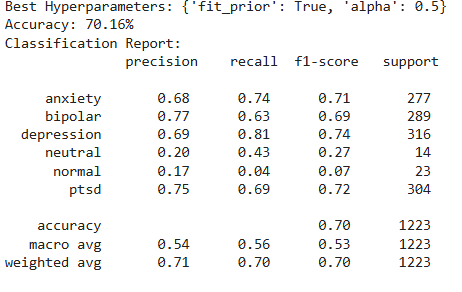
\includegraphics[width=0.8\textwidth]{Images/Output HPT NB.png}  
    \caption{Result of Hyperparameter Tuning on Naive Bayes}
    \label{HPT NB}  % Label for referencing the figure
\end{figure}

\begin{figure}[h!]  
    \centering
    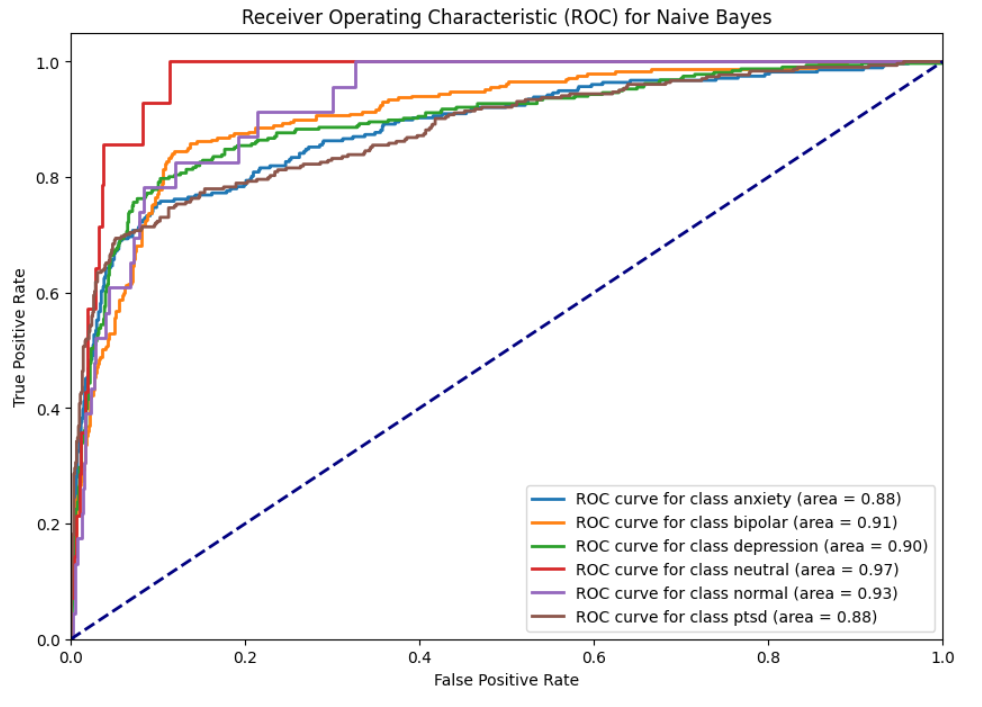
\includegraphics[width=0.8\textwidth]{Images/ROC NB.png}  
    \caption{ROC Curve on Naive bayes}
    \label{ROC NB}  % Label for referencing the figure
\end{figure}

\subssubection{Random Forest}
\noindent
The following code snippet demonstrates the implementation of a Random Forest classifier for classifying mental health issues based on preprocessed text data.

\begin{figure}[h!]  
    \centering
    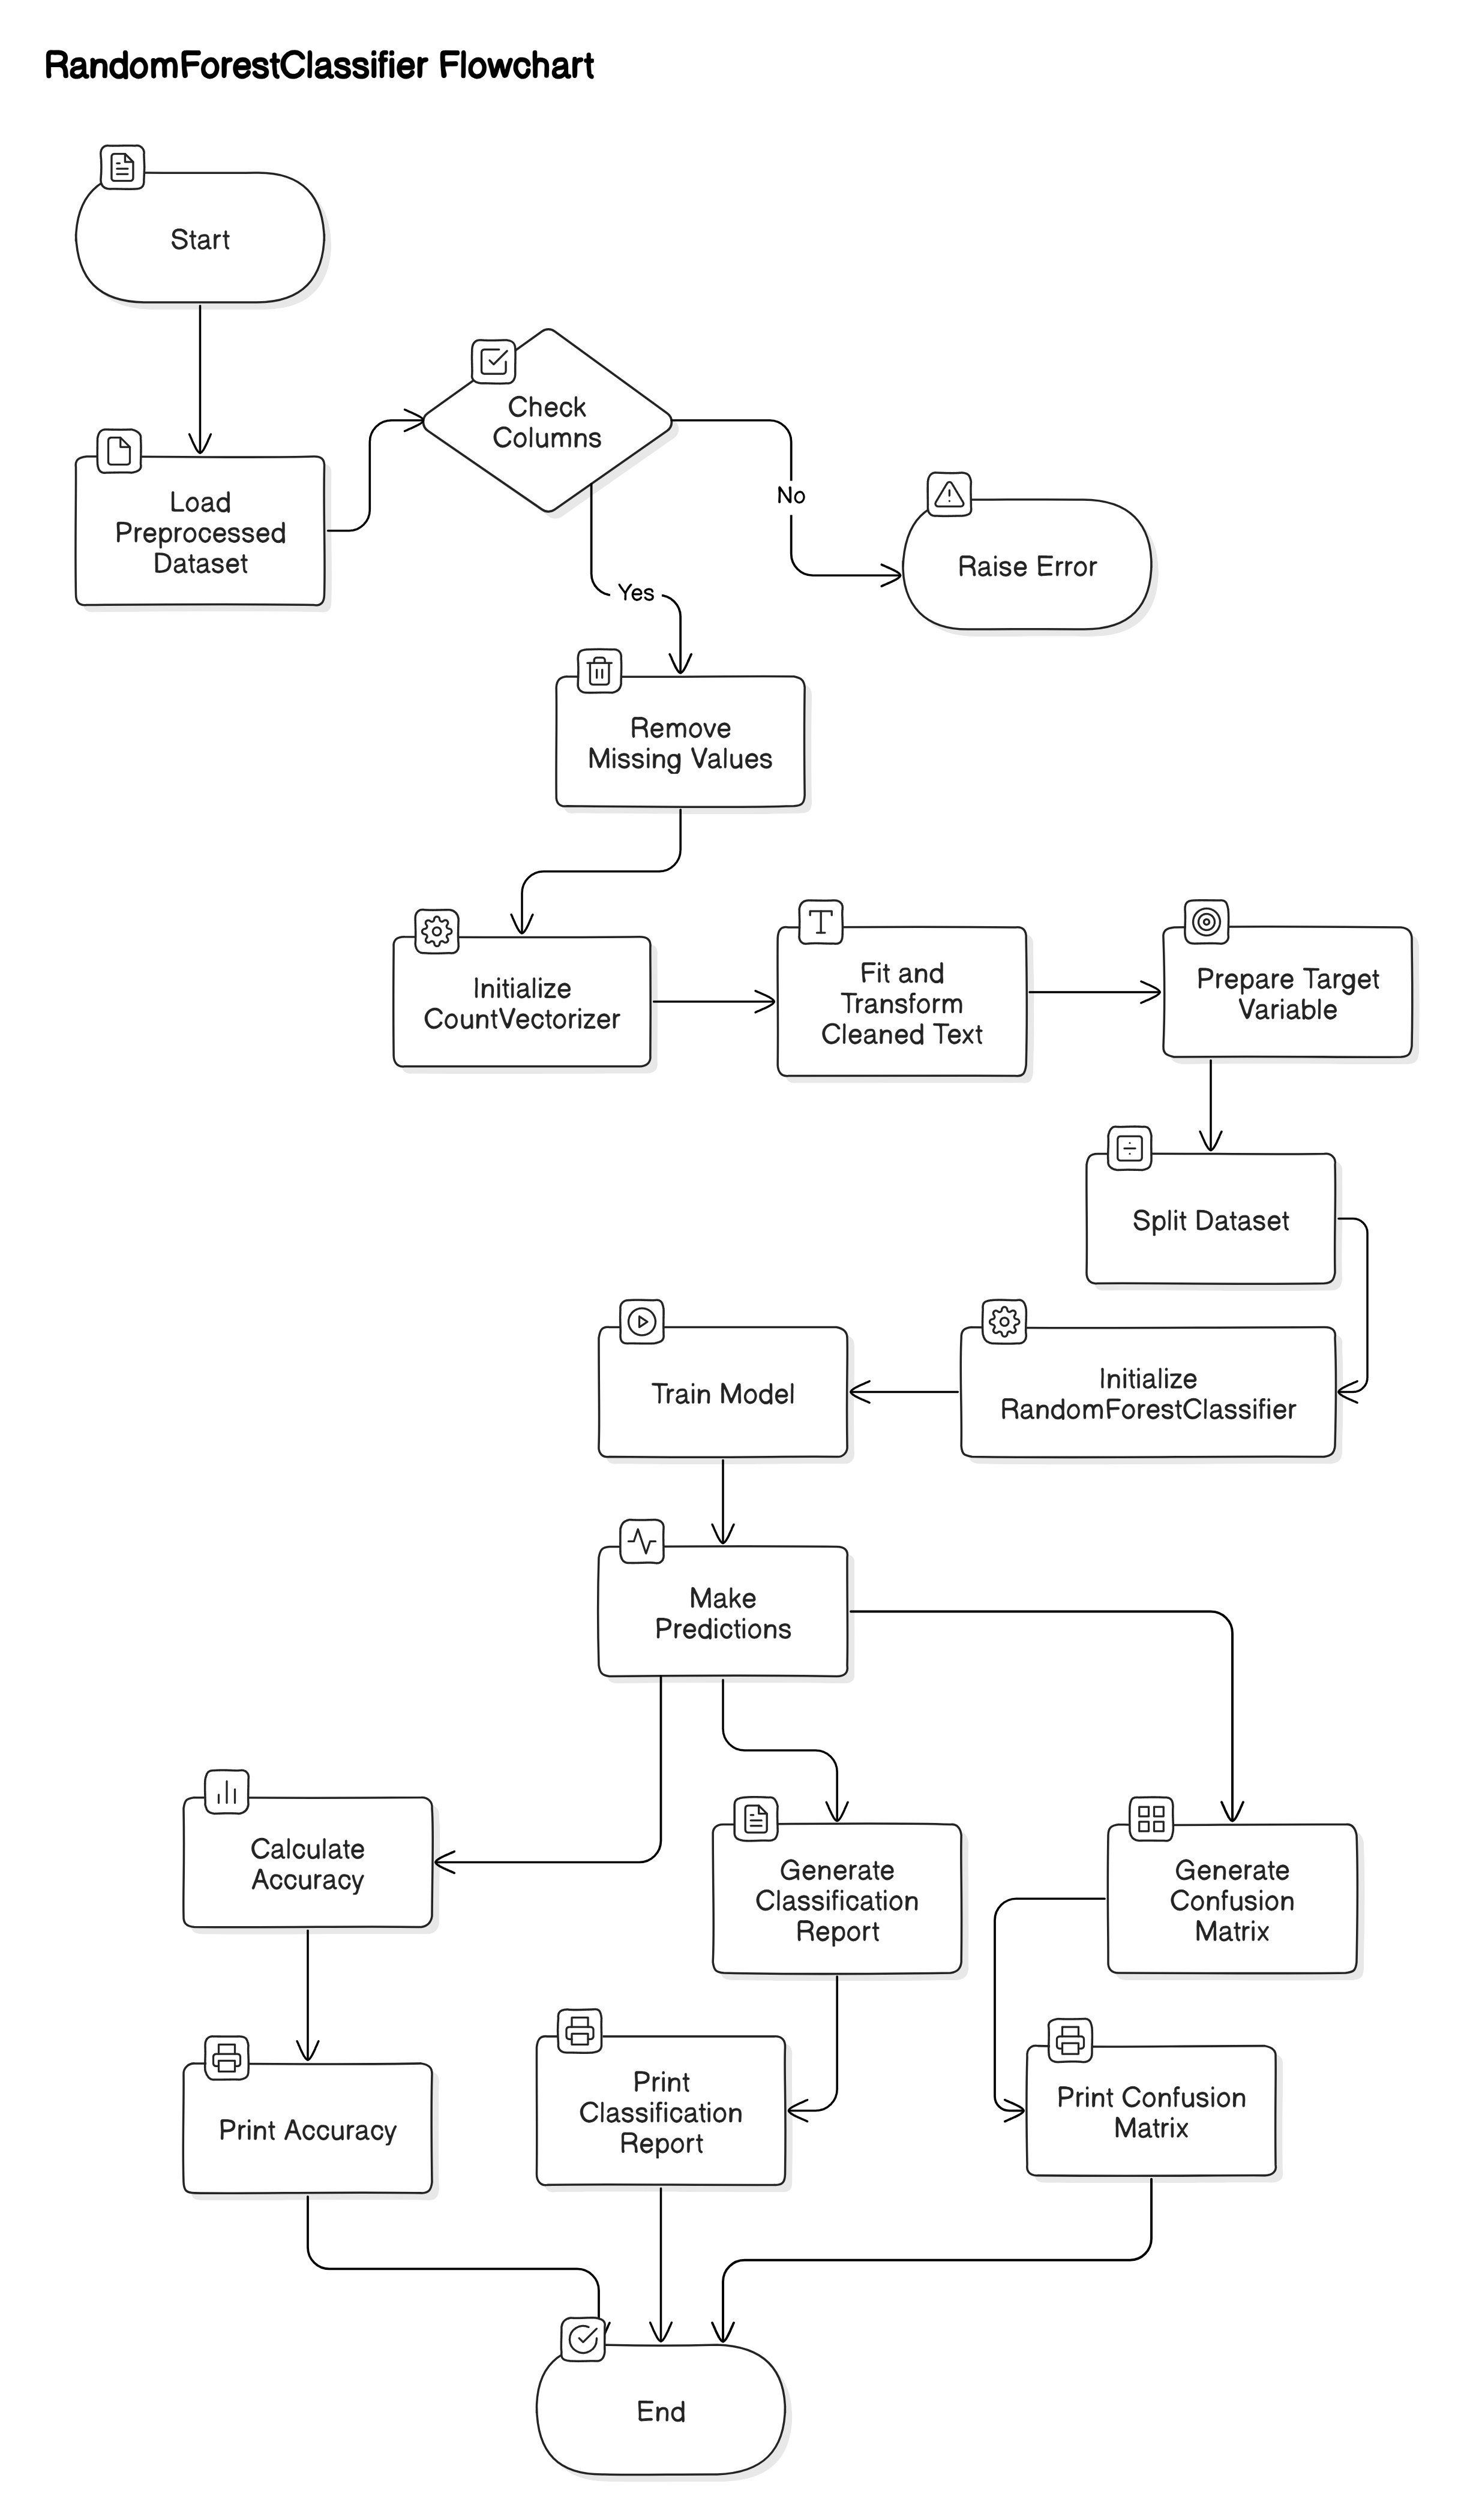
\includegraphics[width=0.6\textwidth]{Images/Random Forest.png}  
    \caption{Random Forest Workflow}
    \label{Random Forest}  % Label for referencing the figure
\end{figure}

\begin{verbatim}
import pandas as pd
from sklearn.model_selection import train_test_split
from sklearn.feature_extraction.text import CountVectorizer
from sklearn.ensemble import RandomForestClassifier
from sklearn.metrics import accuracy_score, classification_report, 
confusion_matrix
dataset = pd.read_csv('preprocessed_mental_health_text.csv')
if 'cleaned_text' not in dataset.columns or 'mental_health_issue' 
not in dataset.columns:
    raise ValueError("The dataset must have 'cleaned_text' and 
    'mental_health_issue' columns.")
dataset.dropna(subset=['cleaned_text'], inplace=True)
vectorizer = CountVectorizer()
X = vectorizer.fit_transform(dataset['cleaned_text'])
y = dataset['mental_health_issue']
X_train, X_test, y_train, y_test = train_test_split(X, y, 
test_size=0.2, random_state=42)
rf_model = RandomForestClassifier(
    n_estimators=3000,
    max_depth=None,
    min_samples_split=20,
    min_samples_leaf=1,
    max_features='sqrt',
    bootstrap=False,
    random_state=42
)
rf_model.fit(X_train, y_train)
y_pred = rf_model.predict(X_test)
accuracy = accuracy_score(y_test, y_pred)
print(f'Accuracy: {accuracy * 100:.2f}%')
print("Classification Report:\n", 
classification_report(y_test, y_pred))
print("Confusion Matrix:\n", confusion_matrix(y_test, y_pred))
\end{verbatim}

\noindent
The code begins by importing the necessary libraries, including \texttt{pandas} for data manipulation and various functions from \texttt{sklearn} for model training and evaluation. It loads the preprocessed dataset from a CSV file named \texttt{preprocessed\_mental\_health\_text.csv} and checks for the presence of the required columns, raising a \texttt{ValueError} if either the \texttt{cleaned\_text} or \texttt{mental\_health\_issue} columns are missing. Rows with missing values in the \texttt{cleaned\_text} column are then removed to ensure data quality. \\

\noindent
The \texttt{CountVectorizer} is initialized to convert the cleaned text into a numerical format, which is stored in \(X\), while the target variable representing mental health issues is assigned to \(y\). The dataset is split into training and testing sets, with 80\% used for training and 20\% for testing. A Random Forest classifier is initialized with specific parameters, including the number of trees (\texttt{n\_estimators}), the minimum number of samples required to split a node (\texttt{min\_samples\_split}), the minimum number of samples in a leaf node (\texttt{min\_samples\_leaf}), and the number of features to consider when looking for the best split (\texttt{max\_features}). The model is then trained using the training data, and predictions are made on the test set. The accuracy of the model is calculated and displayed, along with a classification report and confusion matrix that provide detailed metrics on the model's performance across different categories.

\begin{figure}[h!]  
    \centering
    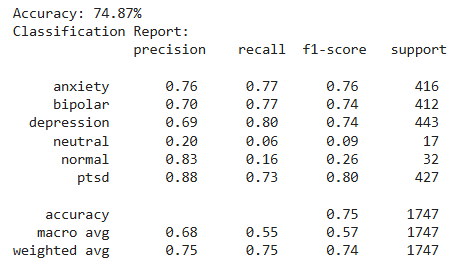
\includegraphics[width=0.9\textwidth]{Images/Output RF.png}  
    \caption{Random Forest Result}
    \label{Random Forest}  % Label for referencing the figure
\end{figure}

\begin{figure}[h!]  
    \centering
    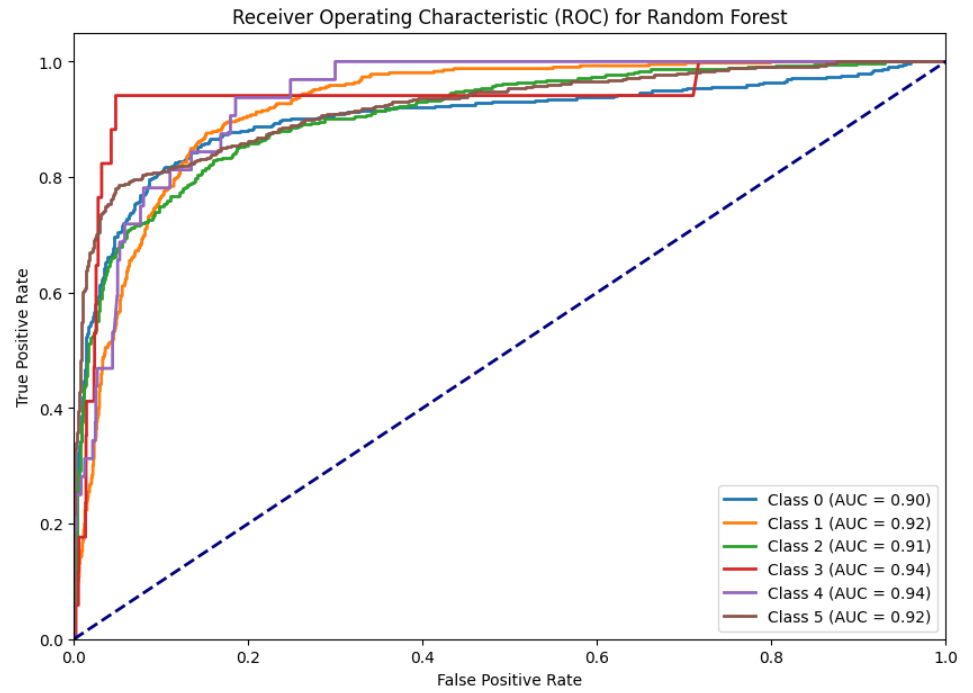
\includegraphics[width=0.9\textwidth]{Images/ROC RF.png}  
    \caption{ROC Curve on Random Forest}
    \label{ROC RF}  % Label for referencing the figure
\end{figure}



% ------------------------- Implementation Ends -----------------------------


% -------------------- Result and Analysis ----------------------------------

\pagebreak

\section{Results and Analysis}
%Prepare the test plans in tabular format, where each Test Case should be represented with distinct id, prefixed with “$\langle$module$\rangle$ “, where module represents the short code of the respective design module. Test Case numbers should be matching as stated in Requirement Matrix.
%\vspace{.1in}

%\noindent

%Appropriate definition of ‘Performance Metrics’, e.g. Classification Accuracy, Mean Squared Error etc. should be included, as applicable. 
%\vspace{.1in}

%\noindent
%Depending on your specific project, test results can be represented as a table of data with a corresponding pie chart / bar chart as needed. Analysis of test results should be discussed in terms of clear bullet points.

\noindent
The metrics used for evaluating the performance of the classification models include Precision, Recall, F1-Score, and Support, along with the Confusion Matrix. These metrics are crucial for assessing how well the models are able to differentiate between various classes, providing insight into their accuracy, ability to capture relevant instances, and the overall balance between precision and recall. By analyzing these metrics, a comprehensive understanding of the model's performance can be obtained, enabling informed decisions for further optimization and tuning.

\subsection{Classification Metrics and Confusion Matrix}

\begin{itemize}
    \item \textbf{Precision:} Precision is the ratio of correctly predicted positive observations to the total predicted positives. It can be calculated as:
    \[
    \text{Precision} = \frac{TP}{TP + FP}
    \]
    where \( TP \) represents True Positives, and \( FP \) represents False Positives.

    \item \textbf{Recall:} Recall is the ratio of correctly predicted positive observations to all observations in the actual class:
    \[
    \text{Recall} = \frac{TP}{TP + FN}
    \]
    where \( TP \) is True Positives, and \( FN \) is False Negatives.

    \item \textbf{F1-Score:} F1-Score is the harmonic mean of Precision and Recall, calculated as:
    \[
    \text{F1-Score} = 2 \times \frac{\text{Precision} \times \text{Recall}}{\text{Precision} + \text{Recall}}
    \]

    \item \textbf{Support:} Support refers to the number of actual occurrences of each class in the dataset:
    \[
    \text{Support} = \text{Number of samples in the true class}
    \]

    \item \textbf{Confusion Matrix:} A confusion matrix is used to evaluate the performance of a classification model. It is structured as follows:
    \[
    \begin{bmatrix}
    TP & FP \\
    FN & TN
    \end{bmatrix}
    \]
    where:
    \begin{itemize}
        \item \( TP \) = True Positives
        \item \( FP \) = False Positives
        \item \( FN \) = False Negatives
        \item \( TN \) = True Negatives
    \end{itemize}
\end{itemize}

\subsection{Results of Logistic Regression and Hyperparameter Tuning}

\begin{center}
    \caption{Logistic Regression Classification Report (Before Hyperparameter Tuning)} \\
\begin{tabular}{|l|c|c|c|c|}
\hline
\textbf{Class} & \textbf{Precision} & \textbf{Recall} & \textbf{F1-Score} & \textbf{Support} \\ \hline
Anxiety        & 0.78               & 0.73            & 0.75              & 416              \\ \hline
Bipolar        & 0.66               & 0.84            & 0.74              & 412              \\ \hline
Depression     & 0.74               & 0.72            & 0.73              & 443              \\ \hline
Neutral        & 0.08               & 0.06            & 0.07              & 17               \\ \hline
Normal         & 0.78               & 0.22            & 0.34              & 32               \\ \hline
PTSD           & 0.83               & 0.74            & 0.78              & 427              \\ \hline
\textbf{Accuracy} & \multicolumn{4}{|c|}{73.78\%} \\ \hline
\textbf{Macro Avg} & 0.64            & 0.55            & 0.57              & 1747             \\ \hline
\textbf{Weighted Avg} & 0.75         & 0.74            & 0.74              & 1747             \\ \hline
\end{tabular} \\

 \vspace{0.25in}% Reduces space between tables

\caption{Logistic Regression Classification Report (After Hyperparameter Tuning)} \\
\begin{tabular}{|l|c|c|c|c|}
\hline
\textbf{Class} & \textbf{Precision} & \textbf{Recall} & \textbf{F1-Score} & \textbf{Support} \\ \hline
Anxiety        & 0.80               & 0.75            & 0.77              & 416              \\ \hline
Bipolar        & 0.66               & 0.85            & 0.74              & 412              \\ \hline
Depression     & 0.75               & 0.74            & 0.75              & 443              \\ \hline
Neutral        & 0.14               & 0.12            & 0.13              & 17               \\ \hline
Normal         & 0.78               & 0.22            & 0.34              & 32               \\ \hline
PTSD           & 0.86               & 0.75            & 0.80              & 427              \\ \hline
\textbf{Accuracy} & \multicolumn{4}{|c|}{75.27\%} \\ \hline
\textbf{Macro Avg} & 0.67            & 0.57            & 0.59              & 1747             \\ \hline
\textbf{Weighted Avg} & 0.76         & 0.75            & 0.75              & 1747             \\ \hline
\end{tabular} \\

  \vspace{0.25in}% Reduces space between tables

\caption{Confusion Matrix for Logistic Regression (After Hyperparameter Tuning)} \\
\begin{tabular}{|l|c|c|c|c|c|c|}
\hline
\textbf{True Class} & \textbf{Anxiety} & \textbf{Bipolar} & \textbf{Depression} & \textbf{Neutral} & \textbf{Normal} & \textbf{PTSD} \\ \hline
Anxiety             & 310              & 45               & 37                  & 2                & 1               & 21            \\ \hline
Bipolar             & 12               & 349              & 35                  & 5                & 1               & 10            \\ \hline
Depression          & 34               & 62               & 327                 & 2                & 0               & 18            \\ \hline
Neutral             & 1                & 8                & 5                   & 2                & 0               & 1             \\ \hline
Normal              & 1                & 23               & 1                   & 0                & 7               & 0             \\ \hline
PTSD                & 31               & 44               & 29                  & 3                & 0               & 320           \\ \hline
\end{tabular}
\end{center}

\subsection{Explanation of the Results (Logistic Regression)}

\textbf{Overall Performance:}

The Logistic Regression model's initial accuracy was \textbf{73.78\%}, which improved to \textbf{75.27\%} after hyperparameter tuning using Randomized Search.

\textbf{Improvement After Hyperparameter Tuning:}

\begin{itemize}
    \item The tuned model showed a slight increase in accuracy, reflecting an improved ability to distinguish between the different mental health classes.
    \item The precision, recall, and F1-scores for most of the individual classes also showed minor improvements.
\end{itemize}

\textbf{Class-wise Analysis:}

\begin{itemize}
    \item \textbf{Anxiety:} The precision and recall improved slightly, indicating better classification of anxiety-related texts.
    \item \textbf{Bipolar:} A notable increase in recall suggests the tuned model became more sensitive to identifying bipolar instances correctly.
    \item \textbf{Depression:} The performance metrics remained relatively stable, showing the model was consistently able to handle depression cases.
    \item \textbf{Neutral \& Normal:} Low precision and recall values indicate that the model struggles to correctly classify these rare classes, likely due to insufficient support (sample size).
\end{itemize}


\begin{figure}[h!]  
    \centering
    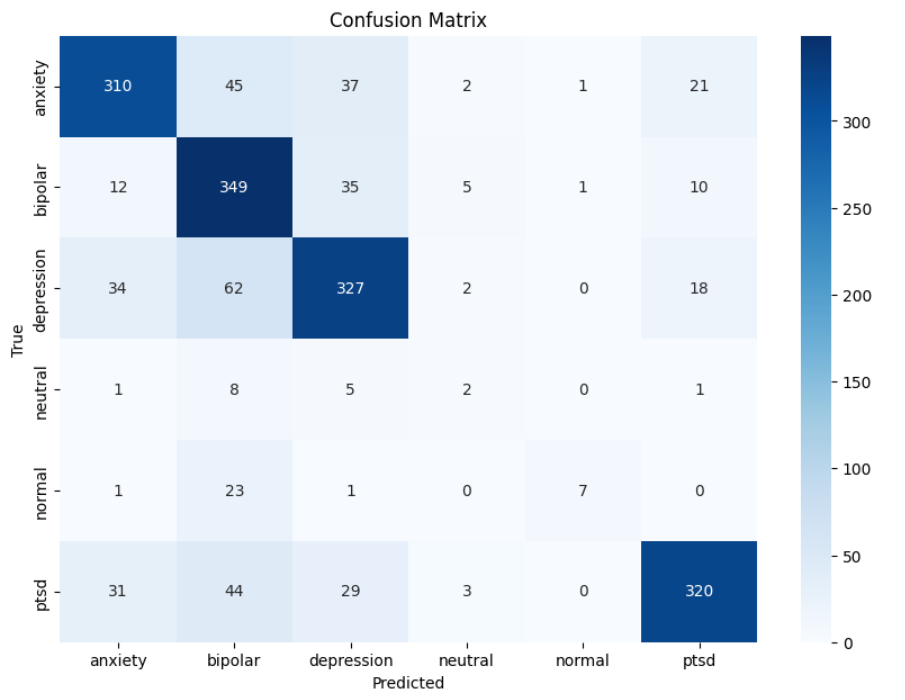
\includegraphics[width=1.0\textwidth]{Images/Confusion Matrix LR.png}  
    \caption{Confusion Matrix for Logistic Regression}
    \label{Project Modules}  % Label for referencing the figure
\end{figure}

\pagebreak
\textbf{Confusion Matrix Analysis:}

\begin{itemize}
    \item The confusion matrix reveals where the model misclassifies different categories. For example:
    \begin{itemize}
        \item \textbf{Anxiety} is often confused with \textbf{Bipolar} and \textbf{Depression}, indicating overlapping features between these classes.
        \item \textbf{PTSD} is more distinct, as shown by a higher number of true positive predictions (320), suggesting that the model can better differentiate this category.
    \end{itemize}
    \item Overall, the confusion matrix helps pinpoint specific classes where the model's predictions are less reliable, providing direction for further improvements.
\end{itemize}




\subsection{Results of K-Nearest Neighbors (KNN) and Hyperparameter Tuning}

\begin{center}
    \caption{KNN Classification Report (Before Hyperparameter Tuning)}
\begin{tabular}{|l|c|c|c|c|}
\hline
\textbf{Class} & \textbf{Precision} & \textbf{Recall} & \textbf{F1-Score} & \textbf{Support} \\ \hline
Anxiety        & 0.60               & 0.36            & 0.45              & 416              \\ \hline
Bipolar        & 0.31               & 0.83            & 0.45              & 412              \\ \hline
Depression     & 0.46               & 0.35            & 0.40              & 443              \\ \hline
Neutral        & 0.00               & 0.00            & 0.00              & 17               \\ \hline
Normal         & 0.29               & 0.06            & 0.10              & 32               \\ \hline
PTSD           & 0.81               & 0.11            & 0.20              & 427              \\ \hline
\textbf{Accuracy} & \multicolumn{4}{|c|}{39.61\%} \\ \hline
\textbf{Macro Avg} & 0.41            & 0.28            & 0.27              & 1747             \\ \hline
\textbf{Weighted Avg} & 0.54         & 0.40            & 0.36              & 1747             \\ \hline
\end{tabular}


\vspace{0.25in}

\caption{Confusion Matrix for KNN (Before Hyperparameter Tuning)}
\begin{tabular}{|l|c|c|c|c|c|c|}
\hline
\textbf{True Class} & \textbf{Anxiety} & \textbf{Bipolar} & \textbf{Depression} & \textbf{Neutral} & \textbf{Normal} & \textbf{PTSD} \\ \hline
Anxiety             & 148              & 221              & 46                  & 0                & 0               & 1             \\ \hline
Bipolar             & 24               & 340              & 42                  & 1                & 3               & 2             \\ \hline
Depression          & 36               & 246              & 154                 & 0                & 0               & 7             \\ \hline
Neutral             & 2                & 14               & 0                   & 0                & 0               & 1             \\ \hline
Normal              & 0                & 30               & 0                   & 0                & 2               & 0             \\ \hline
PTSD                & 38               & 248              & 91                  & 0                & 2               & 48            \\ \hline
\end{tabular}


\vspace{1.5in}

\pagebreak
\caption{KNN Classification Report (After Hyperparameter Tuning)}
\begin{tabular}{|l|c|c|c|c|}
\hline
\textbf{Class} & \textbf{Precision} & \textbf{Recall} & \textbf{F1-Score} & \textbf{Support} \\ \hline
Anxiety        & 0.65               & 0.34            & 0.45              & 416              \\ \hline
Bipolar        & 0.32               & 0.82            & 0.46              & 412              \\ \hline
Depression     & 0.47               & 0.39            & 0.43              & 443              \\ \hline
Neutral        & 0.00               & 0.00            & 0.00              & 17               \\ \hline
Normal         & 0.26               & 0.19            & 0.22              & 32               \\ \hline
PTSD           & 0.73               & 0.15            & 0.24              & 427              \\ \hline
\textbf{Accuracy} & \multicolumn{4}{|c|}{41.27\%} \\ \hline
\textbf{Macro Avg} & 0.40            & 0.31            & 0.30              & 1747             \\ \hline
\textbf{Weighted Avg} & 0.53         & 0.41            & 0.39              & 1747             \\ \hline
\end{tabular}


\vspace{0.25in}

\caption{Confusion Matrix for KNN (After Hyperparameter Tuning)}
\begin{tabular}{|l|c|c|c|c|c|c|}
\hline
\textbf{True Class} & \textbf{Anxiety} & \textbf{Bipolar} & \textbf{Depression} & \textbf{Neutral} & \textbf{Normal} & \textbf{PTSD} \\ \hline
Anxiety             & 143              & 214              & 52                  & 0                & 2               & 5             \\ \hline
Bipolar             & 19               & 337              & 45                  & 1                & 7               & 3             \\ \hline
Depression          & 31               & 223              & 173                 & 1                & 1               & 14            \\ \hline
Neutral             & 0                & 15               & 1                   & 0                & 0               & 1             \\ \hline
Normal              & 0                & 26               & 0                   & 0                & 6               & 0             \\ \hline
PTSD                & 28               & 233              & 97                  & 0                & 7               & 62            \\ \hline
\end{tabular}
\end{center}

\subsection{Explanations for KNN Results}

\begin{itemize}
    \item \textbf{Initial KNN Performance:}
    \begin{itemize}
        \item The initial accuracy of the KNN model is low (\textbf{39.61\%}), indicating that the model struggles to classify the mental health categories effectively.
        \item The recall for the \textbf{Bipolar} class is high (0.83), suggesting that the model is sensitive to detecting bipolar cases but tends to misclassify other categories as bipolar.
        \item Other classes like \textbf{Neutral} and \textbf{Normal} have very low precision and recall, highlighting the model’s inability to distinguish these less frequent categories.
    \end{itemize}

    \item \textbf{After Hyperparameter Tuning:}
    \begin{itemize}
        \item The accuracy improved slightly to \textbf{41.27\%} after tuning with the best hyperparameters \{'weights': 'distance', 'n\_neighbors': 4, 'metric': 'euclidean'\}, indicating minor gains in the classification.
        \item The recall for the \textbf{Anxiety} class decreased, while the precision increased, showing a trade-off in performance.
        \item For the \textbf{Depression} class, both precision and recall increased slightly, indicating that the tuning helped the model distinguish depression cases better.
    \end{itemize}

    \item \textbf{Confusion Matrix Analysis:}
    \begin{itemize}
        \item Many instances of \textbf{Anxiety} and \textbf{Depression} are misclassified as \textbf{Bipolar}, showing overlapping features between these classes.
        \item The class \textbf{PTSD} has a low recall, indicating that most of the PTSD samples are misclassified into other categories.
        \item The class distribution imbalance and similar feature patterns might be contributing to the misclassifications, causing the model to favor more common classes like Bipolar.
    \end{itemize}
\end{itemize}

\begin{figure}[h!]  
    \centering
    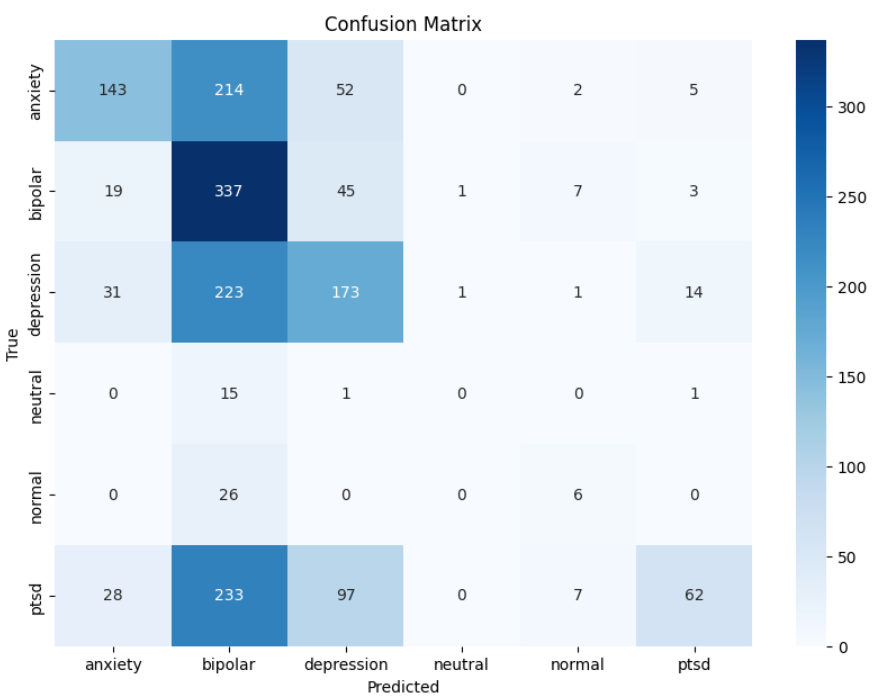
\includegraphics[width=1.0\textwidth]{Images/Confusion Matrix KNN.png}  
    \caption{Confusion Matrix for KNN}
    \label{Confusion Matrix KNN}  % Label for referencing the figure
\end{figure}

\pagebreak
\subsection{Results of Support Vector Machine (SVM) and Hyperparameter Tuning}

\begin{center}
    \caption{SVM Classification Report (Before Hyperparameter Tuning)}
\begin{tabular}{|l|c|c|c|c|}
\hline
\textbf{Class} & \textbf{Precision} & \textbf{Recall} & \textbf{F1-Score} & \textbf{Support} \\ \hline
Anxiety        & 0.70               & 0.70            & 0.70              & 416              \\ \hline
Bipolar        & 0.65               & 0.81            & 0.72              & 412              \\ \hline
Depression     & 0.72               & 0.67            & 0.69              & 443              \\ \hline
Neutral        & 0.19               & 0.18            & 0.18              & 17               \\ \hline
Normal         & 0.62               & 0.25            & 0.36              & 32               \\ \hline
PTSD           & 0.81               & 0.71            & 0.76              & 427              \\ \hline
\textbf{Accuracy} & \multicolumn{4}{|c|}{70.75\%} \\ \hline
\textbf{Macro Avg} & 0.61            & 0.55            & 0.57              & 1747             \\ \hline
\textbf{Weighted Avg} & 0.71         & 0.71            & 0.71              & 1747             \\ \hline
\end{tabular}

\vspace{0.25in}

\caption{Confusion Matrix for SVM (Before Hyperparameter Tuning)}
\begin{tabular}{|l|c|c|c|c|c|c|}
\hline
\textbf{True Class} & \textbf{Anxiety} & \textbf{Bipolar} & \textbf{Depression} & \textbf{Neutral} & \textbf{Normal} & \textbf{PTSD} \\ \hline
Anxiety             & 292              & 45               & 44                  & 2                & 1               & 32            \\ \hline
Bipolar             & 23               & 333              & 37                  & 5                & 3               & 11            \\ \hline
Depression          & 59               & 58               & 296                 & 2                & 0               & 28            \\ \hline
Neutral             & 1                & 7                & 5                   & 3                & 0               & 1             \\ \hline
Normal              & 0                & 24               & 0                   & 0                & 8               & 0             \\ \hline
PTSD                & 41               & 47               & 30                  & 4                & 1               & 304           \\ \hline
\end{tabular}

\vspace{0.25in}

\caption{SVM Classification Report (After Hyperparameter Tuning)}
\begin{tabular}{|l|c|c|c|c|}
\hline
\textbf{Class} & \textbf{Precision} & \textbf{Recall} & \textbf{F1-Score} & \textbf{Support} \\ \hline
Anxiety        & 0.78               & 0.71            & 0.74              & 416              \\ \hline
Bipolar        & 0.61               & 0.83            & 0.70              & 412              \\ \hline
Depression     & 0.75               & 0.70            & 0.72              & 443              \\ \hline
Neutral        & 0.13               & 0.12            & 0.12              & 17               \\ \hline
Normal         & 0.57               & 0.12            & 0.21              & 32               \\ \hline
PTSD           & 0.84               & 0.71            & 0.77              & 427              \\ \hline
\textbf{Accuracy} & \multicolumn{4}{|c|}{72.07\%} \\ \hline
\textbf{Macro Avg} & 0.61            & 0.53            & 0.54              & 1747             \\ \hline
\textbf{Weighted Avg} & 0.73         & 0.72            & 0.72              & 1747             \\ \hline
\end{tabular}

\vspace{0.25in}

\caption{Confusion Matrix for SVM (After Hyperparameter Tuning)}
\begin{tabular}{|l|c|c|c|c|c|c|}
\hline
\textbf{True Class} & \textbf{Anxiety} & \textbf{Bipolar} & \textbf{Depression} & \textbf{Neutral} & \textbf{Normal} & \textbf{PTSD} \\ \hline
Anxiety             & 292              & 45               & 44                  & 2                & 1               & 32            \\ \hline
Bipolar             & 23               & 333              & 37                  & 5                & 3               & 11            \\ \hline
Depression          & 59               & 58               & 296                 & 2                & 0               & 28            \\ \hline
Neutral             & 1                & 7                & 5                   & 3                & 0               & 1             \\ \hline
Normal              & 0                & 24               & 0                   & 0                & 8               & 0             \\ \hline
PTSD                & 41               & 47               & 30                  & 4                & 1               & 304           \\ \hline
\end{tabular}
\end{center}

\subsection{Explanations for SVM Results}

\begin{itemize}
    \item \textbf{Initial SVM Performance:}
    \begin{itemize}
        \item The initial accuracy of the SVM model is \textbf{70.75\%}, indicating a moderate performance in classifying mental health categories.
        \item The \textbf{Bipolar} class has a high recall of 0.81, indicating the model's ability to identify most bipolar cases correctly. However, the precision is lower, showing misclassification with other classes.
        \item The \textbf{Neutral} and \textbf{Normal} classes have low precision and recall values, indicating that the model struggles to identify these minority classes.
    \end{itemize}

    \item \textbf{After Hyperparameter Tuning:}
    \begin{itemize}
        \item The accuracy improved slightly to \textbf{72.07\%} with the best hyperparameters \{'kernel': 'linear', 'gamma': 'scale', 'C': 0.1\}.
        \item The recall for the \textbf{Anxiety} and \textbf{Depression} classes increased, indicating better sensitivity to these categories.
        \item The precision for \textbf{PTSD} also improved, suggesting the model has a clearer distinction for this class after tuning.
    \end{itemize}

    \begin{figure}[h!]  
    \centering
    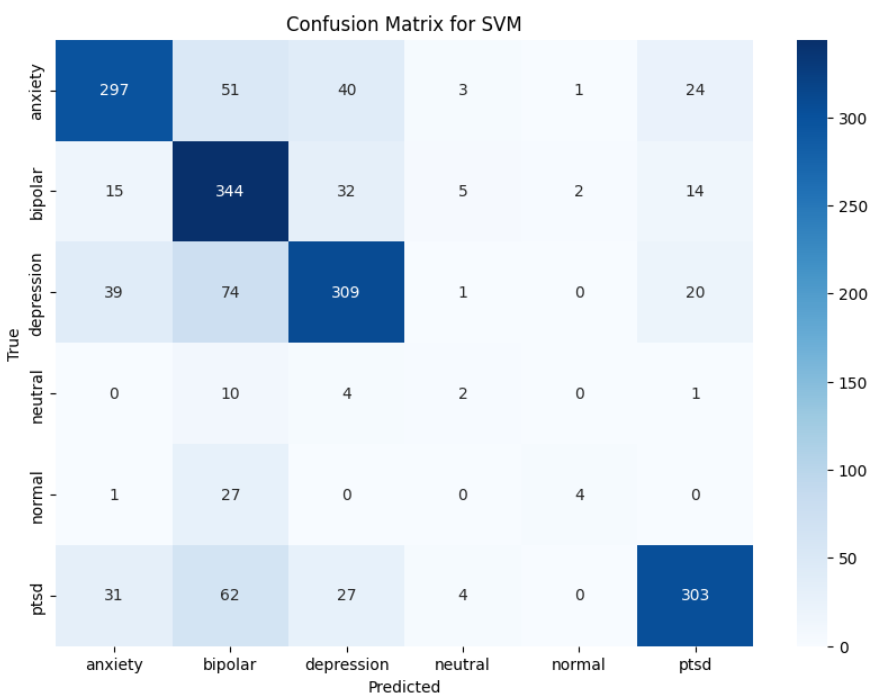
\includegraphics[width=0.8\textwidth]{Images/Confusion Matrix SVM.png}  
    \caption{Confusion Matrix for SVM}
    \label{Confusion Matrix SVM}  % Label for referencing the figure
    \end{figure}

    \item \textbf{Confusion Matrix Analysis:}
    \begin{itemize}
        \item Many instances of \textbf{Anxiety} and \textbf{Depression} are misclassified as \textbf{Bipolar}, showing overlapping features between these classes.
        \item The \textbf{Neutral} and \textbf{Normal} classes have very few true positive predictions, indicating that the SVM model still struggles to capture these less frequent categories.
        \item Overall, the slight improvement in performance after hyperparameter tuning suggests that tuning helped the SVM classifier better balance the trade-offs between precision and recall for most major classes.
    \end{itemize}
\end{itemize}



\subsection{Results of Naive Bayes and Hyperparameter Tuning}

\begin{center}
    \caption{Naive Bayes Classification Report (Before Hyperparameter Tuning)}
\begin{tabular}{|l|c|c|c|c|}
\hline
\textbf{Class} & \textbf{Precision} & \textbf{Recall} & \textbf{F1-Score} & \textbf{Support} \\ \hline
Anxiety        & 0.69               & 0.72            & 0.70              & 416              \\ \hline
Bipolar        & 0.79               & 0.56            & 0.65              & 412              \\ \hline
Depression     & 0.65               & 0.82            & 0.72              & 443              \\ \hline
Neutral        & 0.17               & 0.29            & 0.21              & 17               \\ \hline
Normal         & 0.14               & 0.03            & 0.05              & 32               \\ \hline
PTSD           & 0.73               & 0.72            & 0.72              & 427              \\ \hline
\textbf{Accuracy} & \multicolumn{4}{|c|}{68.92\%} \\ \hline
\textbf{Macro Avg} & 0.53            & 0.52            & 0.51              & 1747             \\ \hline
\textbf{Weighted Avg} & 0.70         & 0.69            & 0.68              & 1747             \\ \hline
\end{tabular}

\vspace{0.25in}

\caption{Confusion Matrix for Naive Bayes (Before Hyperparameter Tuning)}
\begin{tabular}{|l|c|c|c|c|c|c|}
\hline
\textbf{True Class} & \textbf{Anxiety} & \textbf{Bipolar} & \textbf{Depression} & \textbf{Neutral} & \textbf{Normal} & \textbf{PTSD} \\ \hline
Anxiety             & 300              & 14               & 61                  & 8                & 3               & 30            \\ \hline
Bipolar             & 51               & 229              & 78                  & 5                & 0               & 49            \\ \hline
Depression          & 27               & 20               & 362                 & 5                & 1               & 28            \\ \hline
Neutral             & 1                & 6                & 4                   & 5                & 1               & 0             \\ \hline
Normal              & 12               & 2                & 9                   & 1                & 1               & 7             \\ \hline
PTSD                & 46               & 20               & 47                  & 6                & 1               & 307           \\ \hline
\end{tabular}

\vspace{0.25in}

\caption{Naive Bayes Classification Report (After Hyperparameter Tuning)}
\begin{tabular}{|l|c|c|c|c|}
\hline
\textbf{Class} & \textbf{Precision} & \textbf{Recall} & \textbf{F1-Score} & \textbf{Support} \\ \hline
Anxiety        & 0.68               & 0.74            & 0.71              & 277              \\ \hline
Bipolar        & 0.77               & 0.63            & 0.69              & 289              \\ \hline
Depression     & 0.69               & 0.81            & 0.74              & 316              \\ \hline
Neutral        & 0.20               & 0.43            & 0.27              & 14               \\ \hline
Normal         & 0.17               & 0.04            & 0.07              & 23               \\ \hline
PTSD           & 0.75               & 0.69            & 0.72              & 304              \\ \hline
\textbf{Accuracy} & \multicolumn{4}{|c|}{70.16\%} \\ \hline
\textbf{Macro Avg} & 0.54            & 0.56            & 0.53              & 1223             \\ \hline
\textbf{Weighted Avg} & 0.71         & 0.70            & 0.70              & 1223             \\ \hline
\end{tabular}

\vspace{0.25in}

\caption{Confusion Matrix for Naive Bayes (After Hyperparameter Tuning)}
\begin{tabular}{|l|c|c|c|c|c|c|}
\hline
\textbf{True Class} & \textbf{Anxiety} & \textbf{Bipolar} & \textbf{Depression} & \textbf{Neutral} & \textbf{Normal} & \textbf{PTSD} \\ \hline
Anxiety             & 300              & 14               & 61                  & 8                & 3               & 30            \\ \hline
Bipolar             & 51               & 229              & 78                  & 5                & 0               & 49            \\ \hline
Depression          & 27               & 20               & 362                 & 5                & 1               & 28            \\ \hline
Neutral             & 1                & 6                & 4                   & 5                & 1               & 0             \\ \hline
Normal              & 12               & 2                & 9                   & 1                & 1               & 7             \\ \hline
PTSD                & 46               & 20               & 47                  & 6                & 1               & 307           \\ \hline
\end{tabular}    
\end{center}

\subsection{Explanations for Naive Bayes Results}

\begin{itemize}
    \item \textbf{Initial Naive Bayes Performance:}
    \begin{itemize}
        \item The initial accuracy of the Naive Bayes model is \textbf{68.92\%}, indicating moderate classification performance.
        \item The \textbf{Anxiety} and \textbf{Depression} classes have relatively higher recall values, suggesting that the model is sensitive to identifying these categories correctly.
        \item The \textbf{Neutral} and \textbf{Normal} classes have very low precision and recall, indicating that the model struggles to classify these minority classes.
    \end{itemize}

    \item \textbf{After Hyperparameter Tuning:}
    \begin{itemize}
        \item The accuracy increased slightly to \textbf{70.16\%} with the best hyperparameters \{'fit\_prior': True, 'alpha': 0.5\}, showing a minor performance improvement.
        \item The recall for the \textbf{Anxiety} and \textbf{Depression} classes increased, indicating better sensitivity and improved classification for these classes.
        \item However, the precision for the \textbf{Bipolar} class decreased slightly, suggesting a trade-off in correctly identifying true positive cases for this class.
    \end{itemize}
    
    \item \textbf{Confusion Matrix Analysis:}
    \begin{itemize}
        \item Many instances of \textbf{Anxiety} and \textbf{Depression} are misclassified as \textbf{Bipolar}, indicating overlapping feature characteristics between these categories.
        \item The \textbf{Neutral} and \textbf{Normal} classes continue to have very few true positive predictions, highlighting the model’s struggle to capture these less frequent categories.
        \item The increase in recall for major classes like \textbf{Anxiety} and \textbf{Depression} after tuning suggests that the model learned better class-specific distributions.
    \end{itemize}
\end{itemize}

 \begin{figure}[h!]  
    \centering
    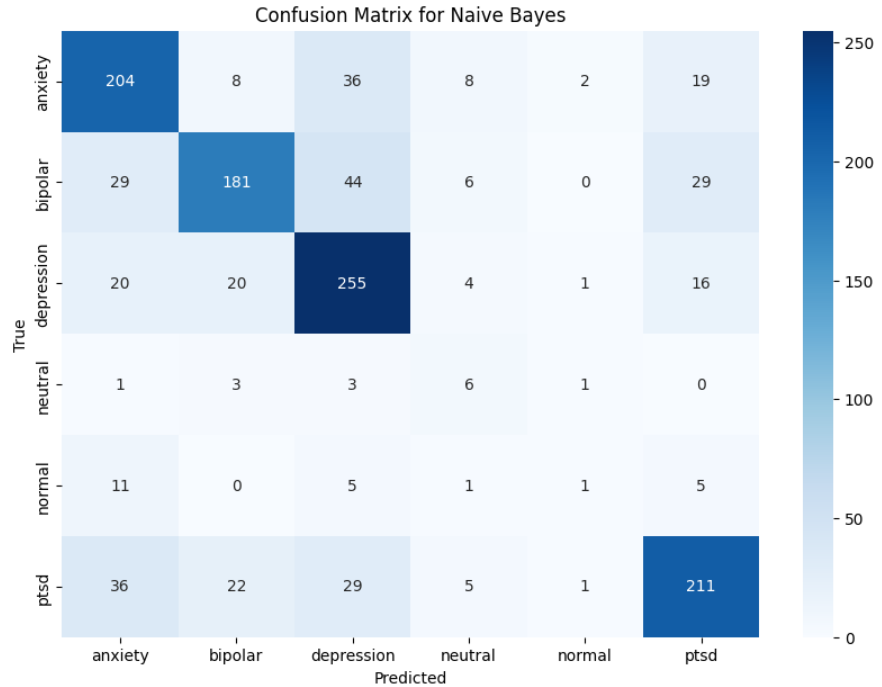
\includegraphics[width=0.8\textwidth]{Images/Confusion Matrix NB.png}  
    \caption{Confusion Matrix for Naive Bayes}
    \label{Confusion Matrix NB}  % Label for referencing the figure
    \end{figure}

\subsection{Results of Random Forest and Hyperparameter Tuning}

\begin{center}
    \caption{Random Forest Classification Report}
\begin{tabular}{|l|c|c|c|c|}
\hline
\textbf{Class} & \textbf{Precision} & \textbf{Recall} & \textbf{F1-Score} & \textbf{Support} \\ \hline
Anxiety        & 0.76               & 0.77            & 0.76              & 416              \\ \hline
Bipolar        & 0.70               & 0.77            & 0.74              & 412              \\ \hline
Depression     & 0.69               & 0.80            & 0.74              & 443              \\ \hline
Neutral        & 0.20               & 0.06            & 0.09              & 17               \\ \hline
Normal         & 0.83               & 0.16            & 0.26              & 32               \\ \hline
PTSD           & 0.88               & 0.73            & 0.80              & 427              \\ \hline
\textbf{Accuracy} & \multicolumn{4}{|c|}{74.87\%} \\ \hline
\textbf{Macro Avg} & 0.68            & 0.55            & 0.57              & 1747             \\ \hline
\textbf{Weighted Avg} & 0.75         & 0.75            & 0.74              & 1747             \\ \hline
\end{tabular}

\vspace{0.25in}

\caption{Confusion Matrix for Random Forest}
\begin{tabular}{|l|c|c|c|c|c|c|}
\hline
\textbf{True Class} & \textbf{Anxiety} & \textbf{Bipolar} & \textbf{Depression} & \textbf{Neutral} & \textbf{Normal} & \textbf{PTSD} \\ \hline
Anxiety             & 319              & 38               & 50                  & 0                & 0               & 9             \\ \hline
Bipolar             & 23               & 319              & 53                  & 2                & 1               & 14            \\ \hline
Depression          & 31               & 41               & 353                 & 0                & 0               & 18            \\ \hline
Neutral             & 1                & 9                & 5                   & 1                & 0               & 1             \\ \hline
Normal              & 3                & 24               & 0                   & 0                & 5               & 0             \\ \hline
PTSD                & 43               & 22               & 49                  & 2                & 0               & 311           \\ \hline
\end{tabular}    
\end{center}

\subsection{Explanations for Random Forest Results}

\begin{itemize}
    \item \textbf{Overall Performance:}
    \begin{itemize}
        \item The accuracy of the Random Forest model is \textbf{74.87\%}, indicating a good level of performance in classifying the different mental health categories.
        \item The \textbf{PTSD} class shows the highest precision (0.88) and recall (0.73), suggesting that the model is effective at identifying PTSD cases correctly.
    \end{itemize}

    \item \textbf{Class-wise Analysis:}
    \begin{itemize}
        \item The precision and recall for the \textbf{Anxiety} and \textbf{Depression} classes are reasonably balanced, indicating that the model is adept at classifying these categories.
        \item The \textbf{Bipolar} class has a slightly lower precision but high recall, suggesting that while the model can identify bipolar instances effectively, it also misclassifies some non-bipolar cases as bipolar.
        \item The performance for the \textbf{Neutral} and \textbf{Normal} classes is concerning, with very low recall and F1-scores, indicating that these classes are often misclassified.
    \end{itemize}

    \begin{figure}[h!]  
    \centering
    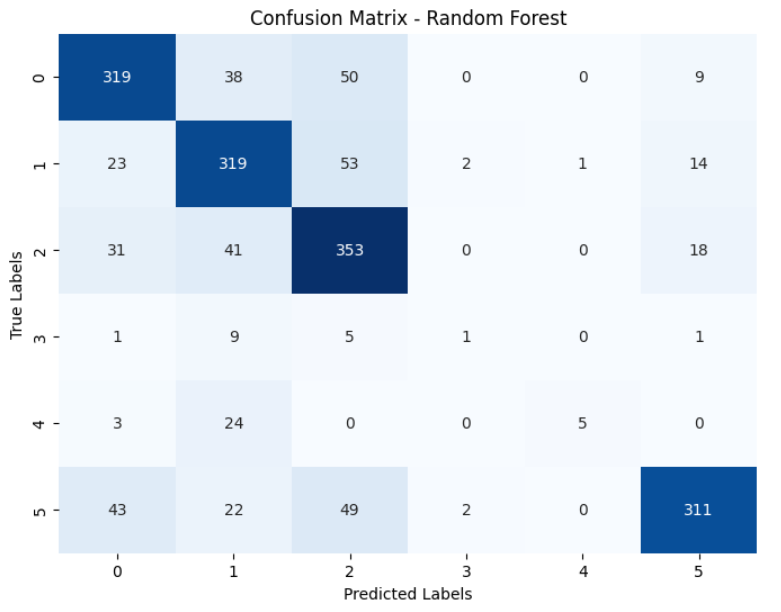
\includegraphics[width=0.9\textwidth]{Images/Confusion Matrix RF.png}  
    \caption{Confusion Matrix for Random Forest}
    \label{Confusion Matrix RF}  % Label for referencing the figure
    \end{figure}

    \item \textbf{Confusion Matrix Analysis:}
    \begin{itemize}
        \item The confusion matrix reveals that many instances of \textbf{Anxiety} and \textbf{Depression} are correctly classified, with a significant number of \textbf{Neutral} instances being misclassified.
        \item The low count for \textbf{Normal} indicates that the model has trouble distinguishing this category, as evidenced by the high number of false positives.
        \item The high number of true positive predictions for \textbf{PTSD} (311) suggests that the Random Forest model is effective in distinguishing PTSD from other classes, likely due to its ability to handle complex feature interactions well.
    \end{itemize}
\end{itemize}

\subsection{Comparison of Different Models}

\begin{center}
    \centering
    \caption{Datasets Overview} \\
    \vspace{0.05in}
    \begin{tabular}{|l|c|c|c|}
    \hline
    \textbf{Dataset} & \textbf{Capacity} & \textbf{Modality} \\ \hline
    Dataset - Reddit  & 12000              & Single            \\ \hline
    Dataset - Twitter  & 900                & Single            \\ \hline
    DS - Reddit + Twitter & 12900          & Single            \\ \hline
    \end{tabular}

    \vspace{0.25in}

\centering
\caption{Comparison of Classification Metrics for Anxiety}
\begin{tabular}{|l|c|c|c|c|}
\hline
\textbf{Model} & \textbf{Precision} & \textbf{Recall} & \textbf{F1-Score} & \textbf{Support} \\ \hline
Logistic Regression & 0.78 & 0.73 & 0.75 & 416 \\ \hline
KNN                & 0.60 & 0.36 & 0.45 & 416 \\ \hline
SVM                & 0.70 & 0.70 & 0.70 & 416 \\ \hline
Naive Bayes        & 0.69 & 0.72 & 0.70 & 416 \\ \hline
Random Forest      & 0.76 & 0.77 & 0.76 & 416 \\ \hline
\end{tabular}

\vspace{0.25in}

\centering
\caption{Comparison of Classification Metrics for Bipolar}
\begin{tabular}{|l|c|c|c|c|}
\hline
\textbf{Model} & \textbf{Precision} & \textbf{Recall} & \textbf{F1-Score} & \textbf{Support} \\ \hline
Logistic Regression & 0.66 & 0.84 & 0.74 & 412 \\ \hline
KNN                & 0.31 & 0.83 & 0.45 & 412 \\ \hline
SVM                & 0.65 & 0.81 & 0.72 & 412 \\ \hline
Naive Bayes        & 0.79 & 0.56 & 0.65 & 412 \\ \hline
Random Forest      & 0.70 & 0.77 & 0.74 & 412 \\ \hline
\end{tabular}

\vspace{0.25in}

\centering
\caption{Comparison of Classification Metrics for Depression}
\begin{tabular}{|l|c|c|c|c|}
\hline
\textbf{Model} & \textbf{Precision} & \textbf{Recall} & \textbf{F1-Score} & \textbf{Support} \\ \hline
Logistic Regression & 0.74 & 0.72 & 0.73 & 443 \\ \hline
KNN                & 0.46 & 0.35 & 0.40 & 443 \\ \hline
SVM                & 0.72 & 0.67 & 0.69 & 443 \\ \hline
Naive Bayes        & 0.65 & 0.82 & 0.72 & 443 \\ \hline
Random Forest      & 0.69 & 0.80 & 0.74 & 443 \\ \hline
\end{tabular}

\vspace{0.25in}

\centering
\caption{Comparison of Classification Metrics for Neutral}
\begin{tabular}{|l|c|c|c|c|}
\hline
\textbf{Model} & \textbf{Precision} & \textbf{Recall} & \textbf{F1-Score} & \textbf{Support} \\ \hline
Logistic Regression & 0.08 & 0.06 & 0.07 & 17 \\ \hline
KNN                & 0.00 & 0.00 & 0.00 & 17 \\ \hline
SVM                & 0.19 & 0.18 & 0.18 & 17 \\ \hline
Naive Bayes        & 0.17 & 0.29 & 0.21 & 17 \\ \hline
Random Forest      & 0.20 & 0.06 & 0.09 & 17 \\ \hline
\end{tabular}


\vspace{0.25in}

\caption{Comparison of Classification Metrics for Normal}
\begin{tabular}{|l|c|c|c|c|}
\hline
\textbf{Model} & \textbf{Precision} & \textbf{Recall} & \textbf{F1-Score} & \textbf{Support} \\ \hline
Logistic Regression & 0.78 & 0.22 & 0.34 & 32 \\ \hline
KNN                & 0.29 & 0.06 & 0.10 & 32 \\ \hline
SVM                & 0.62 & 0.25 & 0.36 & 32 \\ \hline
Naive Bayes        & 0.14 & 0.03 & 0.05 & 32 \\ \hline
Random Forest      & 0.83 & 0.16 & 0.26 & 32 \\ \hline
\end{tabular}

\vspace{0.25in}

\caption{Comparison of Classification Metrics for PTSD}
\begin{tabular}{|l|c|c|c|c|}
\hline
\textbf{Model} & \textbf{Precision} & \textbf{Recall} & \textbf{F1-Score} & \textbf{Support} \\ \hline
Logistic Regression & 0.83 & 0.74 & 0.78 & 427 \\ \hline
KNN                & 0.81 & 0.11 & 0.20 & 427 \\ \hline
SVM                & 0.81 & 0.71 & 0.76 & 427 \\ \hline
Naive Bayes        & 0.73 & 0.72 & 0.72 & 427 \\ \hline
Random Forest      & 0.88 & 0.73 & 0.80 & 427 \\ \hline
\end{tabular}

\vspace{0.25in}

\caption{Comparison of Classification Metrics for Anxiety (After Hyperparameter Tuning)}
\begin{tabular}{|l|c|c|c|c|}
\hline
\textbf{Model} & \textbf{Precision} & \textbf{Recall} & \textbf{F1-Score} & \textbf{Support} \\ \hline
Logistic Regression & 0.80 & 0.75 & 0.77 & 416 \\ \hline
KNN                & 0.65 & 0.34 & 0.45 & 416 \\ \hline
SVM                & 0.78 & 0.71 & 0.74 & 416 \\ \hline
Naive Bayes        & 0.68 & 0.74 & 0.71 & 277 \\ \hline
\end{tabular}

\vspace{0.25in}

\caption{Comparison of Classification Metrics for Bipolar (After Hyperparameter Tuning)}
\begin{tabular}{|l|c|c|c|c|}
\hline
\textbf{Model} & \textbf{Precision} & \textbf{Recall} & \textbf{F1-Score} & \textbf{Support} \\ \hline
Logistic Regression & 0.66 & 0.85 & 0.74 & 412 \\ \hline
KNN                & 0.32 & 0.82 & 0.46 & 412 \\ \hline
SVM                & 0.61 & 0.83 & 0.70 & 412 \\ \hline
Naive Bayes        & 0.77 & 0.63 & 0.69 & 289 \\ \hline
\end{tabular}

\vspace{0.25in}

\caption{Comparison of Classification Metrics for Depression (After Hyperparameter Tuning)}
\begin{tabular}{|l|c|c|c|c|}
\hline
\textbf{Model} & \textbf{Precision} & \textbf{Recall} & \textbf{F1-Score} & \textbf{Support} \\ \hline
Logistic Regression & 0.75 & 0.74 & 0.75 & 443 \\ \hline
KNN                & 0.47 & 0.39 & 0.43 & 443 \\ \hline
SVM                & 0.75 & 0.70 & 0.72 & 443 \\ \hline
Naive Bayes        & 0.69 & 0.81 & 0.74 & 316 \\ \hline
\end{tabular}

\vspace{0.25in}

\caption{Comparison of Classification Metrics for Neutral (After Hyperparameter Tuning)}
\begin{tabular}{|l|c|c|c|c|}
\hline
\textbf{Model} & \textbf{Precision} & \textbf{Recall} & \textbf{F1-Score} & \textbf{Support} \\ \hline
Logistic Regression & 0.14 & 0.12 & 0.13 & 17 \\ \hline
KNN                & 0.00 & 0.00 & 0.00 & 17 \\ \hline
SVM                & 0.13 & 0.12 & 0.12 & 17 \\ \hline
Naive Bayes        & 0.20 & 0.43 & 0.27 & 14 \\ \hline
\end{tabular}

\vspace{0.25in}

\caption{Comparison of Classification Metrics for Normal (After Hyperparameter Tuning)}
\begin{tabular}{|l|c|c|c|c|}
\hline
\textbf{Model} & \textbf{Precision} & \textbf{Recall} & \textbf{F1-Score} & \textbf{Support} \\ \hline
Logistic Regression & 0.78 & 0.22 & 0.34 & 32 \\ \hline
KNN                & 0.26 & 0.19 & 0.22 & 32 \\ \hline
SVM                & 0.57 & 0.12 & 0.21 & 32 \\ \hline
Naive Bayes        & 0.17 & 0.04 & 0.07 & 23 \\ \hline
\end{tabular}

\vspace{0.25in}

\caption{Comparison of Classification Metrics for PTSD (After Hyperparameter Tuning)}
\begin{tabular}{|l|c|c|c|c|}
\hline
\textbf{Model} & \textbf{Precision} & \textbf{Recall} & \textbf{F1-Score} & \textbf{Support} \\ \hline
Logistic Regression & 0.86 & 0.75 & 0.80 & 427 \\ \hline
KNN                & 0.73 & 0.15 & 0.24 & 427 \\ \hline
SVM                & 0.84 & 0.71 & 0.77 & 427 \\ \hline
Naive Bayes        & 0.75 & 0.69 & 0.72 & 304 \\ \hline
\end{tabular}

\end{center}


% ------------------------ Result and Analysis Ends -------------------------



% ------------------------------ Conclusion ---------------------------------

\section{Conclusion}
% State the project benefits. Outline the future scope for improvements.

\subsection{Project Benefits}
\noindent
The project on detecting mental health disorders through social media analysis offers a wide array of significant benefits, both immediate and long-term, across multiple dimensions. First and foremost, it addresses a critical issue in mental health care—early detection and intervention. Social media has become a ubiquitous platform where people express their thoughts, feelings, and emotional states, often unconsciously. By leveraging the vast amounts of data available on social media platforms, our project seeks to tap into this resource to identify early signs of mental health disorders such as anxiety, depression, and more severe conditions like bipolar disorder or schizophrenia. The ability to detect mental health issues through real-time social media data is a game-changer for public health systems, mental health practitioners, and even individuals who may not realize they are at risk. Early detection enables timely intervention, reducing the overall burden of mental health disorders on society by preventing escalation into more severe conditions that often lead to hospitalization, self-harm, or even suicide. In this sense, the project aligns with global health initiatives that emphasize early diagnosis and preventive care. \\

\noindent
Moreover, this project holds significant potential for improving the accuracy and efficiency of mental health diagnostics. Traditional diagnostic methods are often time-consuming, subjective, and reliant on self-reporting, which can lead to underdiagnosis or misdiagnosis. By utilizing machine learning algorithms and natural language processing techniques, our project automates the process of sentiment and behavioral analysis on social media platforms, offering a more objective and data-driven approach. This automated system can process large volumes of data much faster than human professionals, providing insights that would be impossible to glean from manual analysis. The algorithms developed as part of this project can be easily scaled to analyze millions of social media posts, enabling a broader reach in monitoring public mental health trends. Additionally, the project offers practical benefits for mental health professionals, allowing them to focus on treatment and intervention rather than diagnosis. It provides a tool that can be integrated into telehealth systems, offering mental health screening at scale, which is particularly valuable in underserved or rural areas where access to mental health professionals is limited. \\

\noindent
From a technological standpoint, the project offers a host of reusable components and methodologies. The machine learning models developed, the sentiment analysis tools, and the overall data pipeline are designed to be scalable and modular. These components can be adapted and extended to other domains beyond mental health, such as market sentiment analysis, public opinion monitoring, or even detecting harmful behavior like cyberbullying and harassment online. By advancing the state of the art in social media analytics, this project contributes to the growing field of AI-driven health care solutions. Furthermore, it provides a blueprint for future interdisciplinary work that integrates data science, psychology, and public health. \\

\subsection{Future Scope for Improvements}
\noindent
While this project offers numerous immediate benefits, there is substantial room for future enhancements that can broaden its applicability, accuracy, and effectiveness. One of the key areas for improvement lies in the expansion of data sources. Currently, the project focuses on analyzing Twitter sentiment data from Kaggle, which is limited to a specific social media platform and dataset. In the future, incorporating data from other platforms like Facebook, Instagram, Reddit, and even niche forums could provide a more comprehensive understanding of an individual’s mental health status. Different platforms cater to different demographics and social behaviors, and expanding the dataset will allow for a more holistic analysis of mental health indicators across various user bases. Additionally, expanding the dataset to include multilingual posts or integrating language translation capabilities could make the system applicable to a global audience, helping to identify mental health issues in non-English speaking populations. \\

\noindent
Another area ripe for future development is the improvement of the machine learning models used for mental health prediction. Current models, while effective, could benefit from more advanced techniques such as deep learning architectures, which are particularly powerful in handling unstructured data like text and images. For instance, implementing models like transformers or neural networks that can better understand the context and nuance in human language could lead to more accurate predictions. Additionally, incorporating multi-modal data, such as analyzing images and videos along with textual data, could provide richer insights into a user’s mental health state. Emotions and mental health issues are often expressed visually as well, and combining these different data types could significantly improve the system’s accuracy. \\

\noindent
Moreover, future improvements could focus on integrating real-time data analysis capabilities. Currently, our project is based on batch processing of historical data. However, in future iterations, the system could be developed to perform real-time monitoring, offering immediate feedback and potentially alerting health professionals or loved ones when someone shows signs of mental distress. This real-time capability would be invaluable in emergency situations, allowing for immediate intervention. Developing a mobile application or a web-based interface where users can voluntarily connect their social media accounts to monitor their mental health status could also increase user engagement and provide individuals with direct feedback on their well-being. \\

\noindent
Another significant future enhancement could involve incorporating ethical considerations and improving user privacy. As mental health is a sensitive subject, ensuring that the system is designed with robust privacy protections is critical. Future work could focus on using differential privacy or other anonymization techniques to ensure that user data remains confidential while still allowing for effective analysis. Moreover, collaborating with psychologists, ethicists, and legal experts could help refine the system to ensure it adheres to ethical guidelines and avoids potential harm, such as misdiagnosis or privacy violations. \\

\noindent
Lastly, the future scope of this project could include expanding its use in clinical settings. While the current system is primarily designed as a research tool, future iterations could be developed in collaboration with mental health professionals to ensure that it meets clinical standards. By integrating this system with electronic health records or telehealth platforms, it could become a critical tool in mental health care, helping practitioners monitor their patients’ mental health between sessions. This would allow for a more proactive approach to mental health care, potentially reducing the need for emergency interventions and improving overall treatment outcomes.

% ------------------------- Conclusion Ends ----------------------------------



% --------------------------------- References ------------------------------
 \pagebreak

\section{References}

\begin{comment}
    Please list all referred papers / articles / journals / books including your own published papers / patent (if applicable). Listing and citations should follow IEEE standard format.
    
\end{comment}

\vspace{-6em}
\noindent
\renewcommand{\refname}{} % Removes the References title that appears by default
\bibliographystyle{plain}
\bibliography{references}

% -------------------------------- References End ----------------------------





\begin{comment}
    \section{APPENDIX A - Prototypes (optional) \label{sec:proto}}
Provide the filtered part of RM showing selected features for prototype building. State the detailed steps of compilation, execution and setups. Specify prototype details showing codes, screens, test data, sample output and detailed steps of compilation, execution and setups (if any).


    \section{APPENDIX B - Paper publications (optional) \label{sec:pubs}}
If any of your related paper(s) were published in a standard journal / presented in a recognized conference, mention the same including communication on your paper(s) acceptance / publishing note. You should also show appropriate documentation at the time of project viva.
    
\end{comment}




 % ---------------------- SEPERATE FILES FOR CONTENT----

\addcontentsline{toc}{section}{Abstract}

% ------------------------- ABSTRACT ------------------------------------------

\section*{Abstract} 



% Real Input

\noindent
This project employs AI to detect early signs of mental health issues by analyzing text, images, videos, audio, and PDFs shared on platforms like social media. It integrates advanced techniques such as facial expression recognition, image captioning, multilingual support, and psychological assessments like the Rorschach Inkblot Test and Ryff's Wellbeing Scale. Using an ensemble of models (Logistic Regression, SVM, LSTM, etc.), the system achieves 97.63\% accuracy, with a hierarchical model reaching 96.25\% on larger datasets. The web application supports real-time analysis, model retraining, and wellbeing surveys, providing actionable insights through visualizations and mapping mental health concerns to wellbeing parameters for timely interventions.


% ------------------------ ABSTRACT ENDS ------------------------------------

\newpage

% ------------------------ Introduction -------------------------------------

\vspace{2cm}

\section{Introduction}

\begin{comment}
    Briefly introduce the project's overall topic and purpose.
    \vspace{.1in}
    
    \noindent
    Provide specifications of Technical domain (Hardware, Operating System, Software) and Business domain.
    \vspace{.1in}
    
    \noindent
    Provide \textbf{Glossary} / Keywords in a tabular format.
\end{comment}

% Real Input

\subsection{Project Overview}
\noindent
Mental health disorders—including depression, anxiety, bipolar disorder, and PTSD—affect millions worldwide and often go undetected until they manifest in crises. Meanwhile, people increasingly share their thoughts, feelings, and experiences on social media platforms (Reddit, Twitter etc) and in digital documents, leaving behind rich clues about their emotional state. In this work, we develop a multimodal AI framework that ingests text, images, video, and document feeds, uses OCR and deep-learning emotion analysis, and aligns user responses to established well-being scales. By fusing these signals through an ensemble of machine-learning and neural models, our system aims to flag early warning signs of distress and guide users toward timely, personalized support.

\subsection{Project Purpose}
\noindent
Early identification and intervention are critical for mitigating the severity of mental health crises, yet current screening methods often rely on self-report or occasional clinical encounters. This project aims to fill that gap by delivering a continuously learning, data-driven monitoring tool that passively and proactively analyzes digital footprints—from social posts to uploaded documents and survey responses—to surface warning signs long before a crisis point. By putting actionable insights directly into the hands of individuals, caregivers, and healthcare providers, it seeks to enable truly preventative mental-health care at scale.

\pagebreak

\subsection{Technical Domain Specifications}
\vspace{-0.5cm}
\begin{table}[ht]
    \centering
    \begin{tabular}{|>{\raggedright\arraybackslash}p{3cm}|p{10.3cm}|}
      \hline
      \textbf{Domain} & \textbf{Specifications} \\
      \hline
      \textbf{Hardware} &
      Standard machine with $\geq 8$~GB RAM and a multi-core CPU. 
      (Optional: GPU for larger datasets or complex model training.) \\
      \hline
      \textbf{Operating System} &
      Cross-platform support: macOS, Windows 10/11, Linux distributions
      (e.g.\ Ubuntu, Linux Mint). \\
      \hline
      \textbf{Programming Languages} &
      Python 3.x (primary language for ML, data analysis, NLP). \\
      \hline
      \textbf{Libraries / Frameworks} &
      \begin{minipage}[t]{\linewidth}
        \begin{itemize}\setlength\itemsep{0pt}\setlength\parskip{0pt}
          \item \textbf{Data processing:} Pandas, NumPy
          \item \textbf{Machine learning:} Scikit-learn, XGBoost, TensorFlow, Transformers
          \item \textbf{Image/text analysis:} OpenCV, Tesseract, Pytesseract, DeepFace
          \item \textbf{Audio processing:} Librosa, PyDub, SpeechRecognition
          \item \textbf{Social media integration:} PRAW, Tweepy
          \item \textbf{Visualization:} Plotly, Matplotlib
          \item \textbf{Additional tools:} Streamlit, NLTK, Google Generative AI
          \vspace{0.5em}
        \end{itemize}
      \end{minipage} \\
      \hline
      \textbf{Development Environment} &
      Google Colab (cloud execution with optional GPU for large datasets or model training). \\
      \hline
    \end{tabular}
  \end{table}
      

\subsection{Business Domain Specifications}
\vspace{-0.5cm}
\begin{table}[H]
    \centering
    % Increase row height and cell padding
    \renewcommand{\arraystretch}{1.2}
    \setlength{\tabcolsep}{8pt}
    \begin{tabular}{|>{\raggedright\arraybackslash}p{3cm}|>{\raggedright\arraybackslash}p{10cm}|}
      \hline
      \textbf{Stakeholder} & \textbf{Role / Use Case} \\
      \hline
      Mental Health Services &
        Mental health providers, including hospitals and therapy centers, can leverage machine learning to detect early signs of mental disorders from social media data. This proactive approach complements traditional self-reporting and clinical assessments, enabling earlier intervention and support for patients. \\
      \hline
      Social Media Platforms &
        Social media platforms like Twitter and Reddit are key spaces for expressing thoughts and emotions, including mental health struggles. This project’s machine learning models can help these platforms safeguard user well-being by identifying concerns early, while maintaining ethical standards. \\
      \hline
      Public Health Organizations &
        Public health organizations can use real-time social media data to monitor mental well-being, identify trends, and design data-driven interventions. By analyzing language patterns, they can create targeted awareness campaigns that better engage individuals facing mental health challenges. \\
      \hline
    \end{tabular}
\end{table}
  
\pagebreak

\subsection{Glossary / Keywords}
\noindent

\begin{center}

\begin{tabular}{|p{4cm}|p{10cm}|}
  \hline
  \multicolumn{1}{|c|}{\textbf{Term}} & \multicolumn{1}{c|}{\textbf{Definition}} \\

  \hline 
  Natural Language Processing (NLP) & A branch of artificial intelligence focused on the interaction between computers and humans through natural language, including tasks like text analysis. \\

  \hline 
  Retrieval-Augmented Generation (RAG) & A hybrid NLP framework that combines information retrieval and text generation by fetching relevant context from a knowledge base before generating responses, improving factual accuracy and relevance. \\


  \hline 
  Vectorization & The process of converting textual data into numerical form (such as a vector) so that it can be used as input for machine learning models. \\

  \hline 
  Classifier & A machine learning model or algorithm that categorizes or labels data points into predefined classes. \\

  \hline
  Mental Health Disorder & A wide range of conditions that affect mood, thinking, and behavior, including depression, anxiety, schizophrenia, etc. \\

  \hline
  Data Preprocessing & The process of preparing raw data for analysis by cleaning, normalizing, and transforming it into a usable format for machine learning models. \\

  \hline 
  Cross-validation & A model validation technique used to assess how well a model performs by dividing data into training and testing sets multiple times for better accuracy. \\

  \hline
  Precision & In the context of classification, precision refers to the accuracy of positive predictions, calculated as the ratio of true positives to the sum of true and false positives. \\

  \hline
  Recall & In classification, recall measures the ability of a model to identify all relevant instances within a dataset, calculated as the ratio of true positives to the sum of true positives and false negatives. \\
  
  \hline
  PRAW & PRAW (Python Reddit API Wrapper) is a Python library that provides a simple interface to interact with Reddit's API for accessing Reddit data, such as posts, comments, and user information. \\
  \hline
  TesseractOCR & TesseractOCR is an open-source Optical Character Recognition (OCR) engine that extracts text from images with high accuracy; it is widely used for various applications like scanning documents and digitalizing printed text. \\
  \hline
  Depression & There is a difference between depression and mood swings or short-lived emotional reactions to daily experiments; A mental state causing painful symptoms adversely disrupts normal activities (e.g., sleeping). \\
  \hline
\end{tabular}

\begin{tabular}{|p{4cm}|p{10cm}|}
    \hline
    \multicolumn{1}{|c|}{\textbf{Term}} & \multicolumn{1}{c|}{\textbf{Definition}} \\

  \hline
  Anxiety & Several behavioral disturbances are associated with anxiety disorders, including excessive fear and worry. Severe symptoms cause significant impairment in functioning cause considerable distress. Anxiety disorders come in many forms, such as social anxiety, generalized anxiety, panic, etc. \\

  \hline
  Bipolar Disorder & An alternating pattern of depression and manic symptoms is associated with bipolar disorder. An individual experiencing a depressive episode may feel sad, irritable, empty, or lose interest in daily activities. Emotions of euphoria or irritability, excessive energy, and increased talkativeness can all be signs of manic depression. Increased self-esteem, decreased sleep need, disorientation, and reckless behavior may also be signs of manic depression. \\

  \hline
  Post-Traumatic Stress Disorder (PTSD) & In PTSD, persistent mental and emotional stress can occur after an injury or severe psychological shock, characterized by sleep disturbances, constant vivid memories, and dulled response to others and the outside world. \\

  \hline
  DeepFace & DeepFace is a Python library for deep learning-based facial recognition and attribute analysis. It supports several pretrained models and simplifies face recognition tasks, making it suitable for various applications in image analysis. \\

  \hline
  Transformers Module & The Transformers module in Python, developed by Hugging Face, is a library for natural language processing (NLP) tasks like text classification, translation, and summarization, using state-of-the-art models like BERT and GPT. \\

  \hline
  Gemini 2.0 Flash & Gemini 2.0 Flash is a cutting-edge AI model developed by Google, capable of performing advanced generative and analytical tasks across text, image, and other modalities. \\

  \hline
  FFmpeg & FFmpeg is a multimedia framework used for encoding, decoding, transcoding, streaming, and manipulating audio and video files, supporting a wide range of formats and codecs. \\

  \hline
  Hyperparameter Tuning & Hyperparameter tuning involves selecting the best parameters for a machine learning model to optimize its performance on a given task using grid search or random search. \\

  \hline
  Embedding Model & A neural network that transforms individual text inputs into fixed-length vector representations in a continuous semantic space, enabling efficient similarity search and downstream tasks like clustering or retrieval. \\

  \hline
  Cross-Encoder & A model that jointly processes a pair of inputs (e.g., query and document) through a shared encoder and directly produces a relevance score or classification, allowing for richer interaction at the cost of higher compute per pair. \\

  \hline
\end{tabular}
  
\end{center}


% ------------------------------ Introduction Ends ---------------------------

% ------------------------------ Related Studies -----------------------------

\section{Related Studies}

\begin{comment}
    For avoiding plagiarism, citations should be used for all referred texts particularly here and other parts of the document using appropriate numbers within square bracket for all mapped references under \textbf{References} section. You should check any standard journal paper for typical use of citations.     
\end{comment}

\vspace{-2em}

\begin{table}[H]
    \centering
    \label{tab:related_studies}
    \begin{tabularx}{\textwidth}{|p{3.5cm}|X|}
    \hline
    \rowcolor{lightestgray}
    \textbf{Study} & \textbf{Summary} \\ \hline
    Choudhury et al. (2013) & Explored the predictive capabilities of social media content in identifying depression by analyzing Twitter data. They discovered that specific linguistic patterns (e.g., negative emotion words) correlated strongly with self-reported depressive symptoms \cite{Choudhury2013PredictingDV}. \\ \hline
    Guntuku et al. (2017) & Conducted an integrative review which synthesized various methodologies highlighted that social media platforms are rich sources of data, revealing critical information about users' mental health \cite{Guntuku2017DetectingDA}. \\ \hline
    Mathur et al. (2022) & Provided a systematic review analysing machine learning techniques for mental health detection using social media data, leveraging both individual assessments and broader epidemiological studies \cite{Mathur2022MentalHC}. \\ \hline
    Nadeem (2016) & Investigated depression identification on Twitter by developing algorithms to discern emotional cues in tweets revealing that simple text analysis could lead to improvements in identifying mental risks \cite{nadeem2016identifying}. \\ \hline
    AlSagri and Ykhlef (2020) & Introduced a machine learning–based approach for depression detection on Twitter that combined both content and activity features. Their work demonstrated that a fusion of linguistic and behavioral analysis can enhance the accuracy of depression identification \cite{alsagri2020machine}. \\ \hline
    Vaishnavi et al. (2022) & Examined various machine learning algorithms for predicting mental health illnesses using social media posts. Their findings emphasized that certain algorithms outperform others in classifying mental health conditions, underlining the importance of algorithm selection \cite{Vaishnavi_2022}. \\ \hline
    Safa et al. (2023) & Presented a roadmap for predicting mental health using social media, highlighting ongoing challenges such as ethical considerations and data privacy. They stressed the need for a robust ethical framework in research that leverages social media data \cite{safa2023predictingmentalhealthusing}. \\ \hline
    Ensemble learning using transformers for NLP & Provided a comprehensive review of transformer models (BERT, XLNet, RoBERTa, GPT-2, ALBERT) across multiple NLP tasks. The study introduced ensemble learning with these models and demonstrated that ensemble approaches can significantly improve performance over single classifier methods \cite{Zhang_2024}. \\ \hline
    Ensemble hybrid model for depression detection & Proposed an ensemble hybrid model combining SVM and MLP to improve depression prediction accuracy. Addressing class imbalance with SMOTE and cluster sampling, the model achieved an accuracy of 99.39\% and an F1-score of 99.51\%, outperforming previous approaches \cite{Saha2024}. \\ \hline
    Single classifier vs. ensemble ML \newline approaches & Explored various ML techniques to predict mental health issues using survey responses from OSMI. The study compared single classifiers with ensemble approaches, finding that Gradient Boosting achieved the highest accuracy \cite{Chung_2023}. 
    \\ \hline
\end{tabularx}
\end{table}


% ----- add pre frame study

\begin{comment}
    
\begin{figure}[H]  
    \centering
    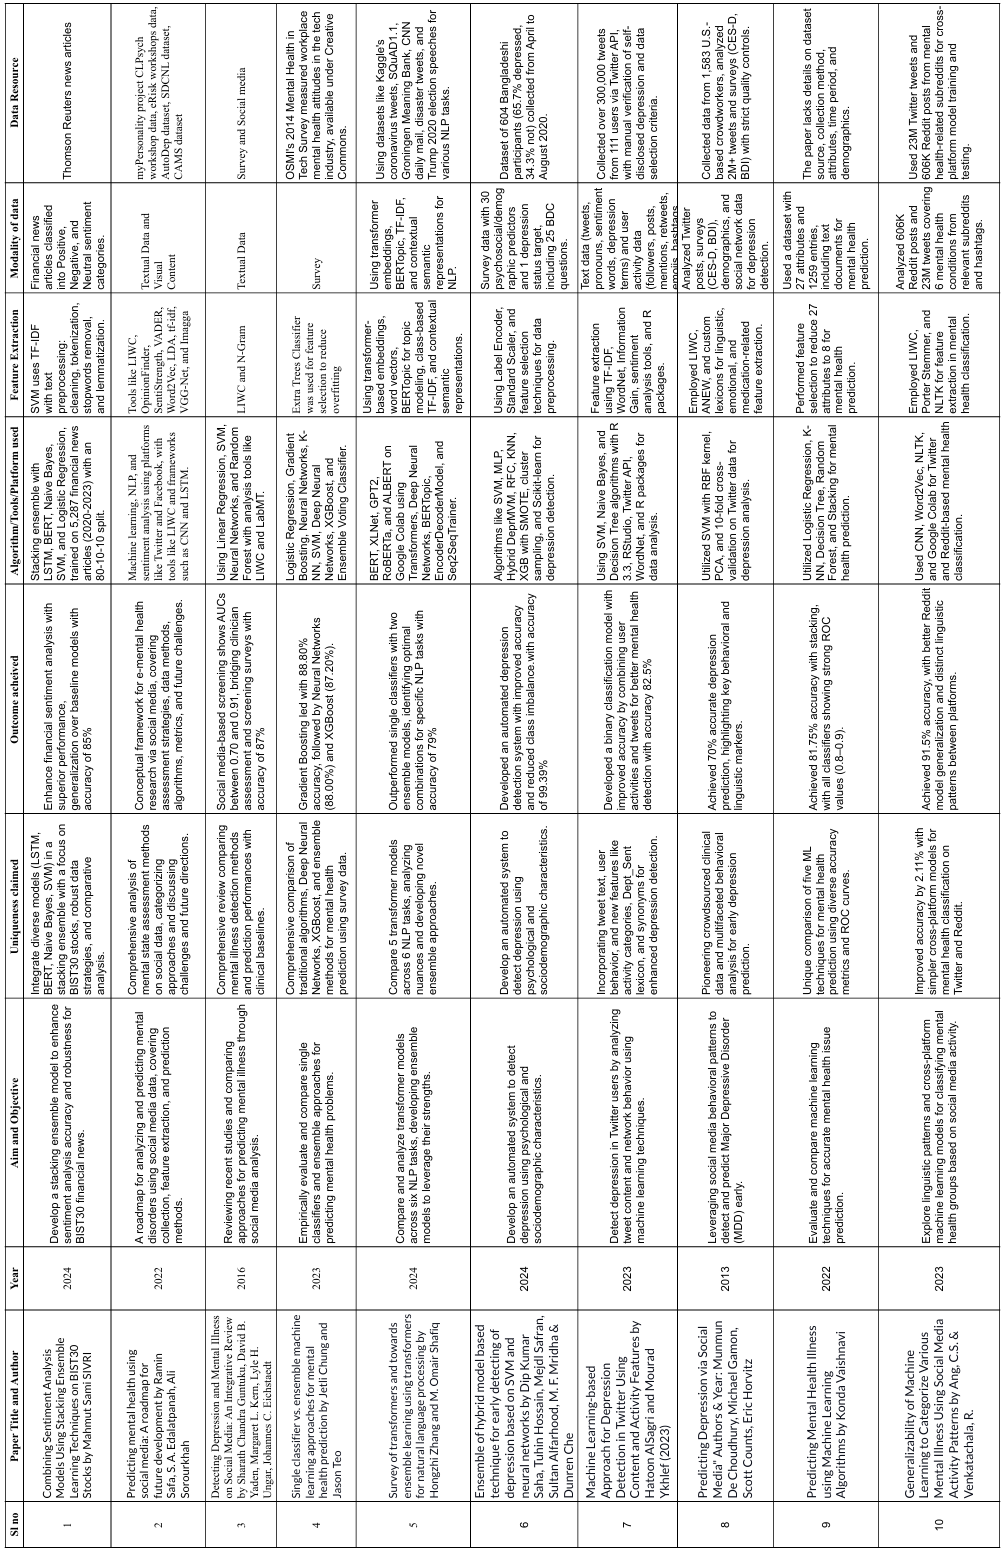
\includegraphics[width=0.95\textwidth]{Images/preframe-study.png}  
    \caption*{Pre frame study review}
    \label{Preframe Study Review}  % Label for referencing the figure
\end{figure}

\end{comment}




\pagebreak

\vspace*{-3.0em}

% Force the rotated table right here
\begin{figure}[H]
\centering

%\caption*{\scriptsize Preframe Study Review}
\hspace*{-0.4cm}
\rotatebox{90}{
\begin{minipage}{\textheight} % Use textheight as width due to rotation
\tiny  % Or \scriptsize or even smaller
\setlength{\arrayrulewidth}{1pt} % Bold vertical lines
\begin{tabular}{|>{\raggedright\arraybackslash}m{0.6cm}|>{\raggedright\arraybackslash}m{2.5cm}|>{\raggedright\arraybackslash}m{0.6cm}|>{\raggedright\arraybackslash}m{2.4cm}|>{\raggedright\arraybackslash}m{2.4cm}|>{\raggedright\arraybackslash}m{2.4cm}|>{\raggedright\arraybackslash}m{2.2cm}|>{\raggedright\arraybackslash}m{2.4cm}|>{\raggedright\arraybackslash}m{2.2cm}|>{\raggedright\arraybackslash}m{2.2cm}|>{\raggedright\arraybackslash}m{2.4cm}|}
%\hlineB{1.0}
%\hlineB{1.4}
\multicolumn{10}{c}{\footnotesize \textbf{PREFRAME STUDY REVIEW}} \\
\hlineB{1.4}
\rowcolor{lightestgray}
\textbf{\rule{0pt}{1.5em} SI No.} & \textbf{\rule{0pt}{1.5em} Paper Title and Author} & \textbf{\rule{0pt}{1.5em} Year} & \textbf{\rule{0pt}{1.5em} Aim and Objective} & \textbf{\rule{0pt}{1.5em} Uniqueness Claimed} & \textbf{\rule{0pt}{1.5em} Outcome Achieved} & \textbf{\rule{0pt}{1.5em} Algorithm/Tools} & \textbf{\rule{0pt}{1.5em} Feature Extraction} & \textbf{\rule{0pt}{1.5em} Modality of Data} & \textbf{\rule{0pt}{1.5em} Data Resource} \\ 
\hlineB{1.4}
1 & Combining Sentiment Analysis Models Using Stacking Ensemble Learning Techniques on BIST30 Stocks by Mahmut Sami SIVRI & 2024 & Develop a stacking ensemble model to enhance sentiment analysis accuracy and robustness for BIST30 financial news. & Integrate diverse models (LSTM, BERT, Naive Bayes, SVM) in a stacking ensemble with a focus on BIST30 stocks, robust data strategies, and comparative analysis. & Enhance financial sentiment analysis with superior performance, generalization over baseline models with accuracy of 85\% & Stacking ensemble with LSTM, BERT, Naive Bayes, SVM, and Logistic Regression, trained on 5,287 financial news articles (2020-2023) with an 80-10-10 split. & SVM uses TF-IDF with text preprocessing: cleaning, tokenization, stopwords removal, and lemmatization. & Financial news articles classified into Positive, Negative, and Neutral sentiment categories. & Thomson Reuters news articles \\ 
\hlineB{1.4}

2 & Predicting mental health using social media: A roadmap for future development by Ramin Safa, S. A. Edalatpanah, Ali Sorourkhah & 2022 & A roadmap for analyzing and predicting mental disorders using social media data, covering collection, feature extraction, and prediction methods. & Comprehensive analysis of mental state assessment methods on social data, categorizing approaches and discussing challenges and future directions. & Conceptual framework for e-mental health research via social media, covering assessment strategies, data methods, algorithms, metrics, and future challenges. & Machine learning, NLP, and sentiment analysis using platforms like Twitter and Facebook, with tools like LIWC and frameworks such as CNN and LSTM. & Tools like LIWC, OpinionFinder, SentiStrength, VADER, Word2Vec, LDA, tf-idf, VGG-Net, and Imagga & Textual Data and Visual Content & myPersonality project CLPsych workshop data, eRisk workshops data, AutoDep dataset, SDCNL dataset, CAMS dataset  \\
\hlineB{1.4}

3 & Detecting Depression and Mental Illness on Social Media: An Integrative Review by Sharath Chandra Guntuku, David B. Yaden, Margaret L. Kern, Lyle H. Ungar, Johannes C. Eichstaedt & 2016 & Reviewing recent studies and comparing approaches for predicting mental illness through social media analysis. & Comprehensive review comparing mental illness detection methods and prediction performances with clinical baselines. & Social media-based screening shows AUCs between 0.70 and 0.91, bridging clinician assessment and screening surveys with accuracy of 87\% & Using Linear Regression, SVM, Neural Networks, and Random Forest with analysis tools like LIWC and LabMT. & LIWC and N-Gram & Textual Data  & Survey and Social media \\
\hlineB{1.4}

4 & Single classifier vs. ensemble machine learning approaches for mental health prediction by Jetli Chung and Jason Teo & 2023 & Empirically evaluate and compare single classifiers and ensemble approaches for predicting mental health problems. & Comprehensive comparison of traditional algorithms, Deep Neural Networks, XGBoost, and ensemble methods for mental health prediction using survey data. & Gradient Boosting led with 88.80\% accuracy, followed by Neural Networks (88.00\%) and XGBoost (87.20\%). & Logistic Regression, Gradient Boosting, Neural Networks, K-NN, SVM, Deep Neural Networks, XGBoost, and Ensemble Voting Classifier. & Extra Trees Classifier was used for feature selection to reduce overfitting & Survey & OSMI's 2014 Mental Health in Tech Survey measured workplace mental health attitudes in the tech industry, available under Creative Commons. \\
\hlineB{1.4}

5 & Survey of transformers and towards ensemble learning using transformers for natural language processing by Hongzhi Zhang and M. Omair Shafiq & 2024 & Compare and analyze transformer models across six NLP tasks, developing ensemble models to leverage their strengths. & Compare 5 transformer models across 6 NLP tasks, analyzing nuances and developing novel ensemble approaches. & Outperformed single classifiers with two ensemble models, identifying optimal combinations for specific NLP tasks with accuracy of 79\% & BERT, XLNet, GPT2, RoBERTa, and ALBERT on Google Colab using Transformers, Deep Neural Networks, BERTopic, EncoderDecoderModel, and Seq2SeqTrainer. & Using transformer-based embeddings, word vectors, BERTopic for topic modeling, class-based TF-IDF, and contextual semantic representations. & Using transformer embeddings, BERTopic, TF-IDF, and contextual semantic representations for NLP. & Using datasets like Kaggle's coronavirus tweets, SQuAD1.1, Groningen Meaning Bank, CNN daily mail, disaster tweets, and Trump 2020 election speeches for various NLP tasks. \\
\hlineB{1.4}

6 & Ensemble of hybrid model based technique for early detecting of depression based on SVM and neural networks by Dip Kumar Saha, Tuhin Hossain, Mejdl Safran, Sultan Alfarhood, M. F. Mridha \& Dunren Che & 2024 & Develop an automated system to detect depression using psychological and sociodemographic characteristics. & Develop an automated system to detect depression using psychological and sociodemographic characteristics. & Developed an automated depression detection system with improved accuracy and reduced class imbalance.with accuracy of 99.39\% & Algorithms like SVM, MLP, Hybrid DeprMVM, RFC, KNN, XGB with SMOTE, cluster sampling, and Scikit-learn for depression detection. & Using Label Encoder, Standard Scaler, and feature selection techniques for data preprocessing. & Survey data with 30 psychosocial/demographic predictors and 1 depression status target, including 25 BDC questions. & Dataset of 604 Bangladeshi participants (65.7\% depressed, 34.3\% not) collected from April to August 2020. \\
\hlineB{1.4}

7 & Machine Learning-based Approach for Depression Detection in Twitter Using Content and Activity Features by Hatoon AlSagri and Mourad Ykhlef & 2023 & Detect depression in Twitter users by analyzing tweet content and network behavior using machine learning techniques. & Incorporating tweet text, user behavior, and new features like activity categories, Dept\_Sent lexicon, and synonyms for enhanced depression detection. & Developed a binary classification model with improved accuracy by combining user activities and tweets for better mental health detection with accuracy 82.5\%. & Using SVM, Naive Bayes, and Decision Tree algorithms with R 3.3, RStudio, Twitter API, WordNet, and R packages for data analysis. & Feature extraction using TF-IDF, WordNet, Information Gain, sentiment analysis tools, and R packages. & Text data (tweets, pronouns, sentiment words, depression terms) and user activity data (followers, posts, mentions, retweets, emojis, hashtags, replies). & Collected over 300,000 tweets from 111 users via Twitter API, with manual verification of self-disclosed depression and data selection criteria. \\
\hlineB{1.4}

8 & Predicting Depression via Social Media" Authors : Munmun De Choudhury, Michael Gamon, Scott Counts, Eric Horvitz & 2013 & Leveraging social media behavioral patterns to detect and predict Major Depressive Disorder (MDD) early. & Pioneering crowdsourced clinical data and multifaceted behavioral analysis for early depression prediction. & Achieved 70\% accurate depression prediction, highlighting key behavioral and linguistic markers. & Utilized SVM with RBF kernel, PCA, and 10-fold cross-validation on Twitter data for depression analysis. & Employed LIWC, ANEW, and custom lexicons for linguistic, emotional, and medication-related feature extraction. & Analyzed Twitter posts, surveys (CES-D, BDI), demographics, and social network data for depression detection. & Collected data from 1,583 U.S.-based crowdworkers, analyzed 2M+ tweets and surveys (CES-D, BDI) with strict quality controls. \\
\hlineB{1.4}


9 & Predicting Mental Health Illness using Machine Learning Algorithms by Konda Vaishnavi & 2022 & Evaluate and compare machine learning techniques for accurate mental health issue prediction. & Unique comparison of five ML techniques for mental health prediction using diverse accuracy metrics and ROC curves. & Achieved 81.75\% accuracy with stacking, with all classifiers showing strong ROC values (0.8–0.9). & Utilized Logistic Regression, K-NN, Decision Tree, Random Forest, and Stacking for mental health prediction. & Performed feature selection to reduce 27 attributes to 8 for mental health prediction. & Used a dataset with 27 attributes and 1259 entries, including text documents for mental health prediction. & Not mentioned \\
\hlineB{1.4}

10 & Generalizability of Machine Learning to Categorize Various Mental Illness Using Social Media Activity Patterns by Ang, C.S. \& Venkatachala, R. & 2023 & Explore linguistic patterns and cross-platform machine learning models for classifying mental health groups based on social media activity. & Improved accuracy by 2.11\% with simpler cross-platform models for mental health classification on Twitter and Reddit. & Achieved 91.5\% accuracy, with better Reddit model generalization and distinct linguistic patterns between platforms. & Used CNN, Word2Vec, NLTK, and Google Colab for Twitter and Reddit-based mental health classification. & Employed LIWC, Porter Stemmer, and NLTK for feature extraction in mental health classification. & Analyzed 606K Reddit posts and 23M tweets covering 6 mental health conditions from relevant subreddits and hashtags. & Used 23M Twitter tweets and 606K Reddit posts from mental health-related subreddits for cross-platform model training and testing. \\
\hlineB{1.4}

% Add more rows as needed
\end{tabular}
\end{minipage}
}
%\vspace{0.1em}
%\caption*{Preframe Study Review}
\end{figure}

% ----------------------------- Related Studies End --------------------------

\pagebreak

% ------------------------------ Related Studies -----------------------------


% -------------- Problem Definition and Preleminaries ------------------------
\pagebreak
\section{Problem Definition and Preliminaries}

\begin{comment}
    State the problem you have solved. Define the boundaries of your project. What was included (scope) and what was not (exclusions)?
\vspace{.1in}

\noindent
Briefly explain the methods you used to conduct your research or complete the project. Were there specific tools, techniques or libraries employed?
\end{comment}

\subsection{Context and Background}
\noindent
Mental health disorders affect approximately 1 in 8 people globally. Social media platforms like Reddit and Twitter offer vast amounts of real-time data reflecting mental health struggles, but the unstructured nature of this data poses challenges for effective identification and categorization of specific disorders.

\subsection{Objective and Challenges}
\noindent
The primary objective is to develop a system that uses NLP and machine learning to analyze Reddit and Twitter posts for detecting mental health disorders like depression, anxiety, bipolar disorder, and PTSD. It seeks to \textbf{classify posts} accurately and provide \textbf{data-driven insights} into mental health trends for researchers, professionals, and policymakers.

\begin{itemize}
    \item \textbf{Data Variability}: Social media posts vary in structure, style, and language.
    \item \textbf{Imbalanced Data}: Uneven distribution of mental issues can impact model training.
    \item \textbf{Cultural Nuances}: Mental health discussions differ across cultures.
    \item \textbf{Privacy and Ethics}: Analyzing social media data raises concerns about user privacy.
\end{itemize}


\subsection{Scope, Exclusions and Assumptions}
\noindent
The scope of the project is to develop a multimodal AI framework to detect mental disorders from social media inputs using ML and NLP. It analyzes text, images, videos, PDFs, dynamic responses to image shown and Reddit/Twitter data via APIs, classifying inputs into Normal, Anxiety, Depression, Bipolar, or PTSD using a Reddit dataset. Finally an association is created between mental health disorder and mental wellbeing paramters from Ryff's Psychological Well-being Scale.

\vspace{1em}

\noindent
This project excludes real-time sentiment analysis, platform-specific features like hashtags or subreddits, and ethical implications of data ownership. It also does not analyze comments, metadata, or Reddit/Twitter-specific elements, focusing solely on detecting mental health disorders from user profiles and mapping them to wellbeing insights, though the dataset has been made solely from Reddit posts from various subreddits.

\vspace{1em}

\noindent
The project assumes that the Reddit dataset obtained via PRAW represents diverse mental health discussions and that user posts accurately reflect emotions. NLP techniques are presumed effective for sentiment classification, and selected ML models (Logistic Regression, SVM, Naïve Bayes, LSTM, Transformer, XGBoost) are expected to perform optimally. Social media sentiments are considered valid proxies for public mental health perceptions. Data preprocessing is assumed sufficient to reduce noise, and ethical standards are maintained to protect user privacy. The user responses well-being surveys are considered valid for updating the association matrix between mental health disorders and well-being parameters.


% ----------- Problem Definition and Preliminaries ends ----------------------

% ----------------------- Proposed Solution ----------------------------------

\section{Proposed Solution}

\vspace{-1.5em}

\begin{table}[H]
    \centering
    \caption*{Special Contributions}
    \vspace{-0.5em}
    \label{tab:project_components}
    \begin{tabularx}{\textwidth}{|p{4cm}|>{\raggedright\arraybackslash}X|}
    \hline
    \rowcolor{lightestgray}
    \textbf{Component} & \textbf{Description} \\ \hline
    Dataset Acquisition & Reddit data was sourced using PRAW from relevant subreddits (Normal, Depression, Anxiety, Bipolar, PTSD). Extensive preprocessing ensured data integrity. \\ \hline
    Text Vectorization & TF-IDF and Bag-of-Words were used to convert text into numerical format via Scikit-learn, enabling efficient feature extraction and model training. Other vectorization techniques like Word2Vec, LIWC, and N-Grams were also explored. \\ \hline
    Machine Learning \newline Models & Logistic Regression, SVM, Naïve Bayes, LSTM, Transformer, and XGBoost were implemented for multi-class classification of mental health conditions. \\ \hline
    Model Evaluation & Accuracy, precision, recall, and F1-score were used to assess performance. Confusion matrices and ROC curves were generated for detailed model evaluation. \\ \hline
    Insights \& \newline Recommendations & Findings inform mental health professionals and policymakers on probable issues and provide well-being insights. \\ \hline
    Documentation \& \newline Reproducibility & Detailed documentation ensures usability, including methodology, code, and instructions for result reproduction. \\ \hline
    \end{tabularx}
\end{table}

\vspace{-0.5cm}

\begin{table}[H]
    \centering
    \caption*{Reusable Components}
    \vspace{-0.5em}
    \label{tab:modules_functions}
    \begin{tabularx}{\textwidth}{|p{4cm}|X|}
    \hline
    \rowcolor{lightestgray}
    \textbf{Module / Function} & \textbf{Description} \\ \hline
    Data Collection \newline Functions & Modular functions designed for data collection, which can be reused across different platforms. \\ \hline
    Data Preprocessing Module & A component that cleans data by removing duplicates and empty rows, and adds a separate column for cleaned texts. \\ \hline
    Machine and Deep Learning Model \newline Functions & Functions for implementing Logistic Regression, Naïve Bayes, Support Vector Machine, Random Forest, XGBoost, Long Short Term Memory, and Transformer algorithms. These functions enable easy retraining on varying datasets and feature various evaluation metrics to assess model performance. \\ \hline
    Deployment Function & A separate function that contains the main Python file for creating a web-based application on Streamlit Cloud, including the necessary requirements and package dependencies for deployment. \\ \hline
    \end{tabularx}
\end{table}

% ----------------------- Proposed Solution Ends -----------------------------

% ----------------------- Project Planning -----------------------------------

\section{Project Planning}

\begin{comment}
    State your project plan with up-to-date tasks, dependencies, timelines and milestones. You may paste your plan appropriately from MS Project etc. 
\vspace{.1in}

\noindent
Include cost analysis if applicable. 
\vspace{.1in}

\noindent
Mention the software life cycle model you followed.    
\end{comment}

\subsection{Software Life Cycle Model}
\noindent
In developing the project, I adopted an iterative approach to the Waterfall model, enabling a structured yet flexible framework for managing the various phases of the project. The project plan outlines specific tasks, dependencies, timelines, and milestones to ensure a systematic progression towards the final goal of analyzing social media posts for mental health disorder detection. \\

\noindent
The Iterative Waterfall model was chosen for this project due to its structured approach while allowing for iterative revisions and refinements. Unlike the traditional Waterfall model, which emphasizes a linear progression through distinct phases, the iterative variant permits revisiting earlier stages based on findings and feedback. This flexibility is particularly beneficial in data-driven projects where insights gained during the analysis may necessitate adjustments to earlier stages, such as refining requirements or enhancing data preparation techniques. \\

\noindent
In this project, the iterative nature of the Waterfall model facilitated ongoing improvement and adaptation throughout the development process. For example, initial results from the model evaluation phase may prompt a revisit to data preprocessing to enhance data quality or to explore alternative modeling techniques. This approach ultimately fosters a more robust final product, ensuring that the developed system meets the dynamic needs of mental health disorder detection in social media posts. \\

\noindent
The key feature of the iterative approach is the feedback loop that exists between the phases. For instance, after completing the testing phase, if certain models do not meet performance expectations, the project can loop back to the implementation phase. This allows for modifications to the models, preprocessing techniques, or even revisiting the requirements to ensure alignment with the project's objectives. \\

\noindent
The project is divided into distinct phases:

\begin{itemize}
    \item \textbf{Requirement Gathering and Analysis} :
    \noindent
    This initial phase involved understanding the project's goals, objectives, and stakeholder expectations. It spanned approximately two weeks, culminating in a detailed requirements document that guided the subsequent stages.
    \item \textbf{Data Collection and Preparation} :
    \noindent
    Utilizing a Twitter sentiment dataset from Kaggle and Reddit API, the data collection phase was executed over a week. This included downloading the dataset, examining its structure, and performing data cleaning and prepossessing to ensure its suitability for analysis.
    \item \textbf{Model Development} :
    \noindent
    This phase, lasting about three weeks, included the creation of a Bag of Words model, splitting the dataset into training and test sets, and implementing various machine learning algorithms such as k-Nearest Neighbors (k-NN) and Support Vector Machines (SVM) for sentiment classification.
    \item \textbf{Model Evaluation} :
    \noindent
    Following model development, a week was allocated for rigorous testing and validation of the models, ensuring they met the required accuracy benchmarks. This phase involved using performance metrics such as accuracy, precision, recall, and F1-score to evaluate the models' effectiveness.
    \item \textbf{Final Deployment and Documentation} :
    \noindent
    The last phase, spanning two weeks, focused on deploying the best-performing model and creating comprehensive documentation. This included user manuals and technical documentation to facilitate future maintenance and enhancements.
\end{itemize}

% Insert SDLC Images
\begin{figure}[h!]  
    \centering
    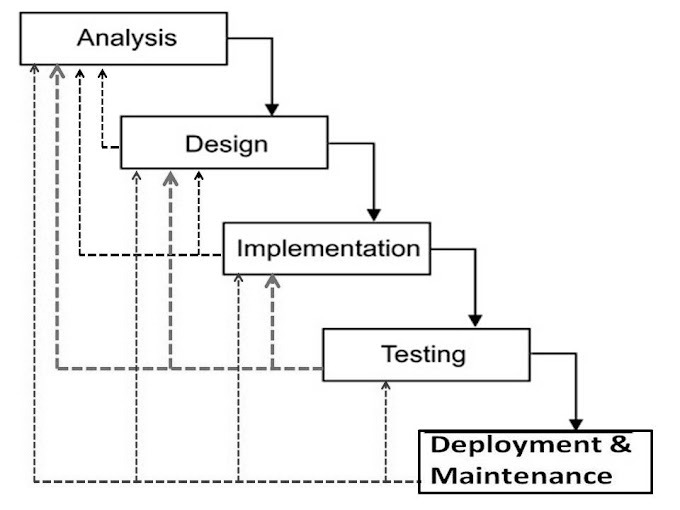
\includegraphics[width=0.6\textwidth]{Images/01 Life_cycle.jpg}  
    \caption{Iterative Waterfall Model}
    \label{Iterative Waterfall Model}  % Label for referencing the figure
\end{figure}


\subsection{Dependencies and Milestones} 
\noindent
Key dependencies were identified for successful project progression. For instance, completion of the data preparation phase was critical before proceeding to model development. Milestones were established at the end of each phase to ensure accountability and track progress. The successful completion of the requirement gathering phase marked the first milestone, followed by the data preparation phase, and so on.

\subsection{Scheduling}
\noindent
Effective scheduling is crucial to the success of any project, as it establishes a clear timeline for tasks, milestones, and dependencies. In the context of our project on detecting mental health disorders through social media analysis, a detailed schedule has been developed to guide the project from inception to completion. This schedule includes specific tasks such as requirement gathering, data preprocessing, model implementation, testing, and deployment, each with clearly defined deadlines. The iterative nature of our chosen methodology allows for flexibility within the schedule, enabling adjustments based on testing outcomes and stakeholder feedback. Key milestones, such as the completion of data analysis, model validation, and user acceptance testing, have been identified to monitor progress and ensure timely delivery of the final product. By utilizing project management tools, such as Microsoft Project, we can visualize and track the progress of tasks, manage resources effectively, and maintain open communication among team members, ensuring that the project stays on schedule and meets its objectives. This proactive approach to scheduling enhances our ability to deliver a high-quality solution that aligns with our goals and stakeholder expectations.

% Insert MS Project Plan Image
\begin{figure}[h!]  
    \centering
    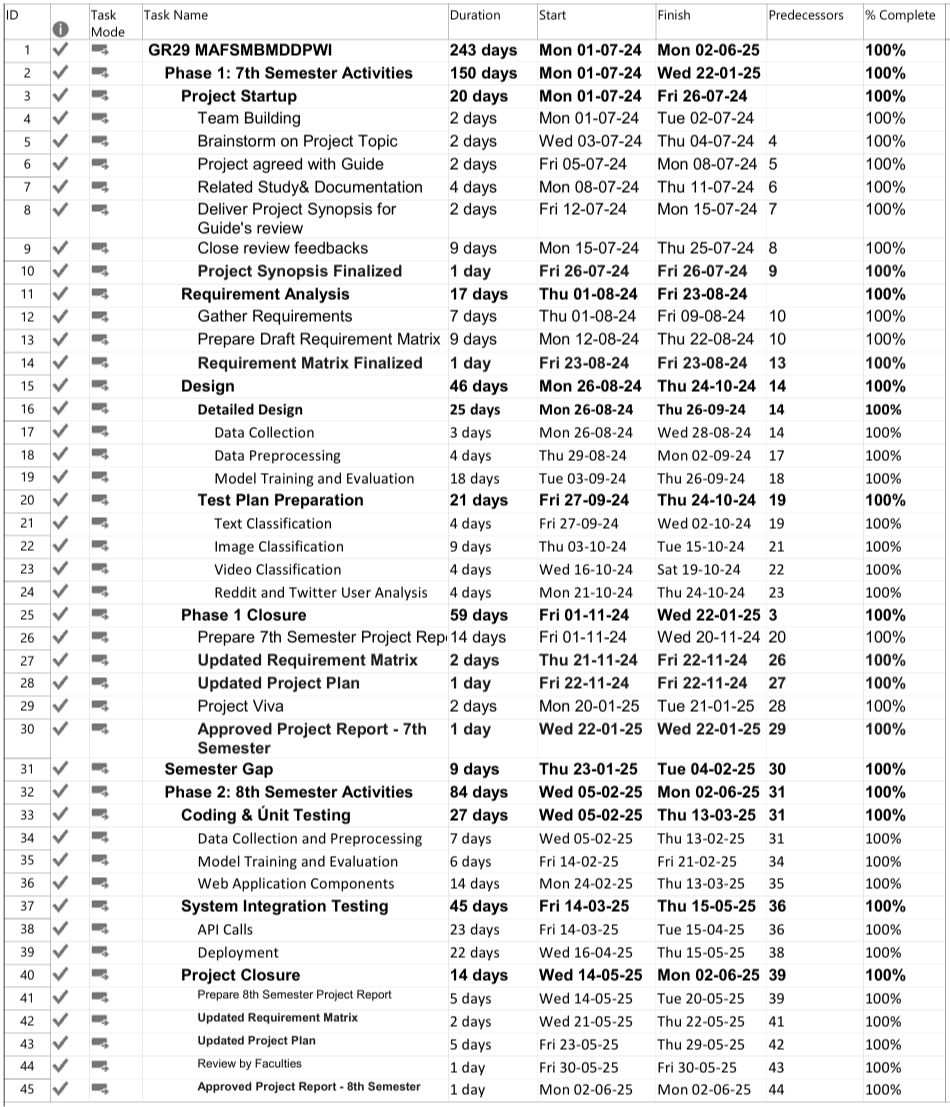
\includegraphics[width=1.0\textwidth]{Images/MS Project Plan Sem 7.png}  
    \caption{Project Plan}
    \label{Project Plan}  % Label for referencing the figure
\end{figure}


\begin{figure}[h!]  
    \centering
    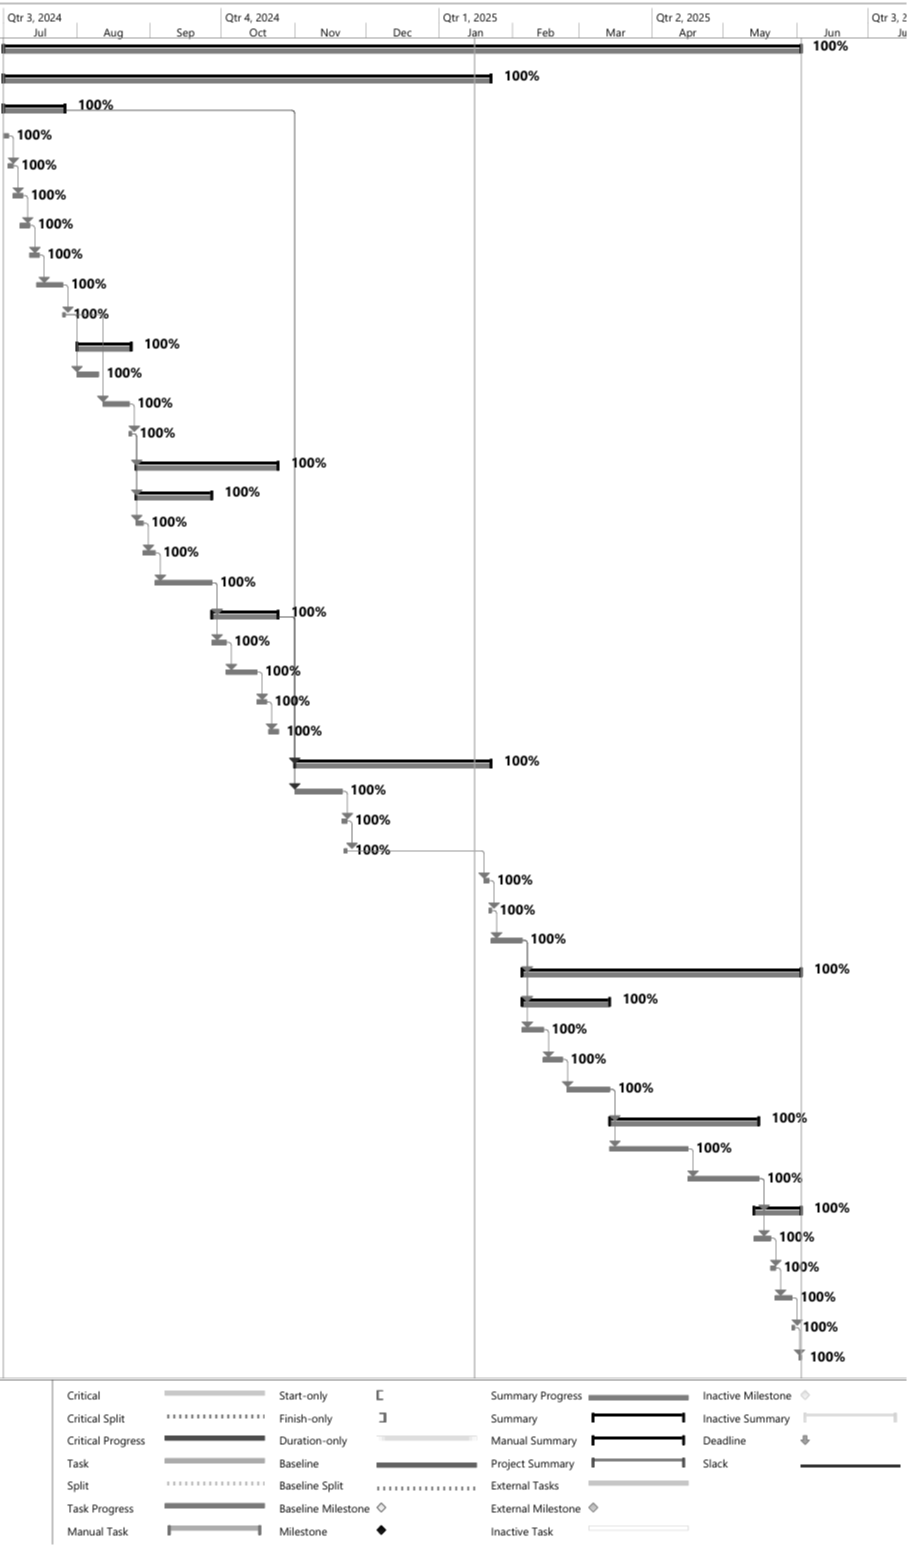
\includegraphics[width=0.79\textwidth]{Images/Gantt Chart.png}  
    \caption{Gantt Chart}
    \label{Gantt Chart}  % Label for referencing the figure
\end{figure}

\pagebreak
% ----------------------- Project Planning ends ------------------------------

% --------------------- Requirement Analysis ---------------------------------
\pagebreak

\section{Requirement Analysis}

\subsection{Requirement Matrix}
% For Requirement Matrix, latest excel should be pasted and formatted here.
\begin{figure}[H]  
    \centering
    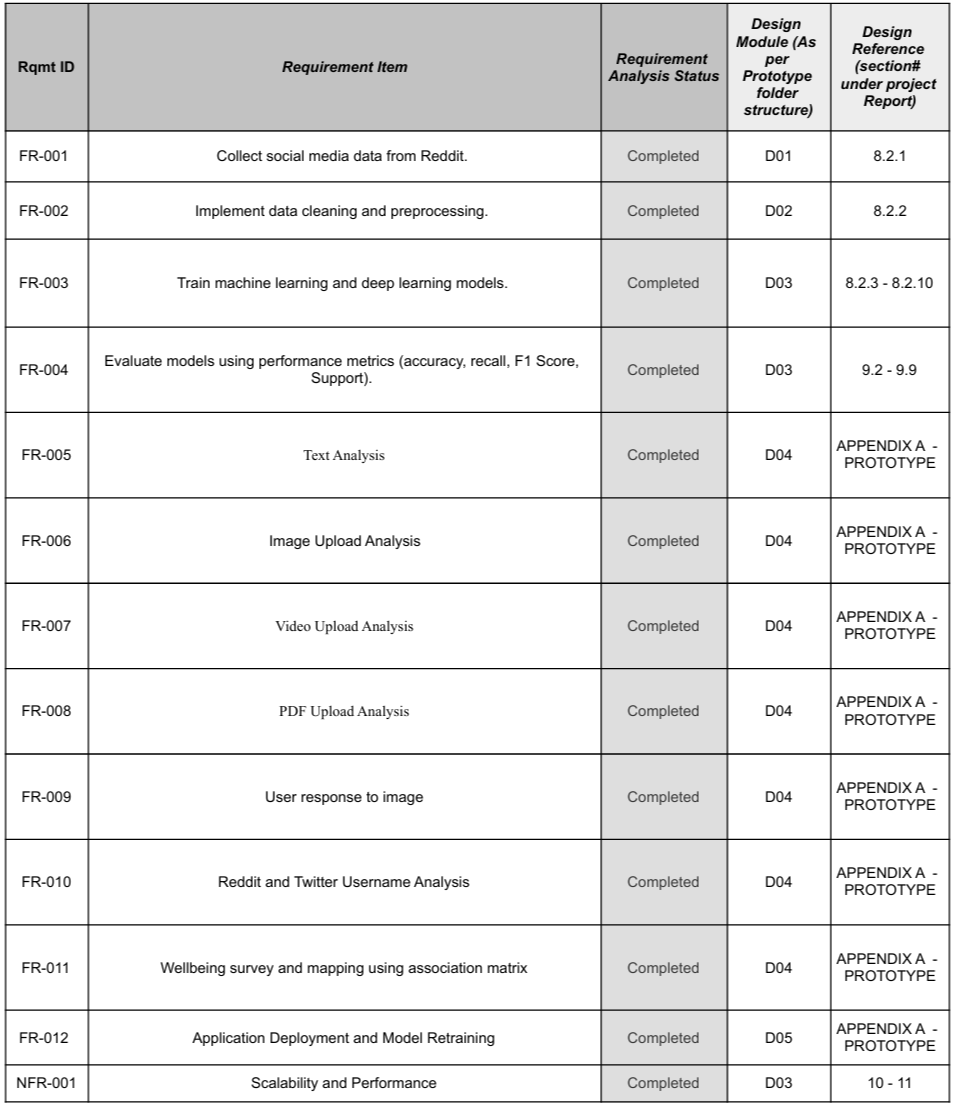
\includegraphics[width=1.0\textwidth]{Images/Requirement Matrix.png}  
    \caption{Requirement Matrix}
    \label{Requirement Matrix}  % Label for referencing the figure
\end{figure}

\pagebreak

\subsection{Requirement Elaboration}
% Create separate sections for separate areas of requirement as in Requirement Matrix. 
% \vspace{.1in}

% \noindent
% For \textbf{Requirement Elaboration}, titles of s6.2.1, 6.2.2 etc. should be with the name of respective requirement areas. Your focus should be on: “What is needed in the system?” Requirement IDs should match with the ID column under Requirement Matrix.

\begin{table}[H]
    \centering
    \renewcommand{\arraystretch}{1.2}
    \begin{tabularx}{\textwidth}{|c|X|X|X|}
        \hline
        \rowcolor{lightestgray}
        \textbf{No} & \textbf{Requirement} & \textbf{Input} & \textbf{Output} \\
        \hline
        FR-001 & Collect social media data from Reddit & API queries & Raw text data \\
        \hline
        FR-002 & Implement data cleaning and preprocessing & Raw text data & Cleaned, structured text \\
        \hline
        FR-003 & Train machine learning and deep learning models & Preprocessed data & Trained \newline models \\
        \hline
        FR-004 & Evaluate models using performance metrics & Trained models & Accuracy, Recall, F1 Score \\
        \hline
        FR-005 & Text Analysis & User text input & Mental disorder classification \\
        \hline
        FR-006 & Image Upload Analysis & Uploaded image & Extracted text, emotions for classification \\
        \hline
        FR-007 & Video Upload Analysis & Uploaded video & Extracted frames, emotions and text for classification \\
        \hline
        FR-008 & PDF Upload Analysis & Uploaded PDF & Extracted text and analysis \\
        \hline
        FR-009 & User response to image & User input & Mental Disorder classification based on input text \\
        \hline
        FR-010 & Reddit and Twitter \newline Username Analysis & Username input & Mental disorder trends across the top posts \\
        \hline
        FR-011 & Wellbeing survey and mapping using \newline association matrix & Survey responses & Mental health insights \\
        \hline
        FR-012 & Application \newline Deployment and Model Retraining & Updated dataset & Improved/updated model accuracy within the web application\\
        \hline
        \hline
        NFR-001 & Scalability and \newline Performance & Handling bigger dataset and subset models for a global ensemble model & Maintaining overall accuracy and response time \\
        \hline
    \end{tabularx}
    \caption*{\textbf{Functional and Non-Functional Requirements}}
\end{table}

\pagebreak
% -------------------- Requirement Analysis Ends -----------------------------

% ----------------------------- Design ---------------------------------------

\section{Design}

\subsection{Technical Environment}
% Mention minimum hardware configuration, software tools and package details.
\noindent
The technical environment for the project "Multimodal AI Framework for Social Media Based Mental Disorder Detection and Personalized Wellbeing Insights" comprises a combination of hardware, software, and tools that enable smooth data analysis, machine learning model training, and deployment. Below is an overview of the minimum hardware configuration, software tools, and package details necessary to carry out this project effectively. 

\begin{table}[h]
    \centering
    \renewcommand{\arraystretch}{1.2}
    \begin{tabular}{|c|p{12cm}|}
        \hline
        \textbf{Component} & \textbf{Specification} \\
        \hline
        Processor & Intel Core i5 (or equivalent) with a base clock speed of at least 2.5 GHz. A multi-core processor is preferred for parallel processing, essential for model training and data preprocessing. \\
        \hline
        RAM & 8 GB recommended for handling data loading, cleaning, and transformation. For large datasets, 16 GB is ideal to prevent memory overflow and processing delays. \\
        \hline
        Storage & Minimum 256 GB SSD recommended. SSD offers faster read/write speeds, significantly improving dataset loading times, especially for large datasets like Reddit-based social media posts. \\
        \hline
        GPU & Not necessary for basic ML tasks like Logistic Regression or SVM. For deep learning, an NVIDIA GTX 1060 with 4 GB VRAM or higher is advantageous. \\
        \hline
        Operating System & Windows 10 (64-bit) or higher, macOS 10.13 (High Sierra) or higher, or any stable Linux distribution (e.g., Ubuntu 18.04 or higher). The OS should support ML libraries and project tools. \\
        \hline
    \end{tabular}
    \caption*{\textbf{Minimum Hardware Configuration}}
\end{table}


\begin{table}[h]
    \centering
    \renewcommand{\arraystretch}{1.2}
    \begin{tabular}{|c|p{12cm}|}
        \hline
        \textbf{Library/Package} & \textbf{Description} \\
        \hline
        Python & Primary programming language for data processing and model training. \\
        \hline
        pandas & Data manipulation and preprocessing. \\
        \hline
        scikit-learn & Machine learning models and evaluation tools. \\
        \hline
        Streamlit & Web framework for deploying interactive ML applications. \\
        \hline
        pyngrok & Creates secure tunnels for sharing local applications. \\
        \hline
        Google Colab & Cloud-based Python environment with GPU/TPU support. \\
        \hline
        PRAW & Access and retrieve Reddit data via API. \\
        \hline
        pytesseract & OCR library for extracting text from images. \\
        \hline
        Pillow & Image processing and handling library. \\
        \hline
    \end{tabular}
    \caption*{\textbf{Libraries and Packages Used}}
    \label{tab:libraries}
\end{table}

\pagebreak
\begin{table}[H]
    \centering
    \renewcommand{\arraystretch}{1.2}
    \begin{tabular}{|c|p{12cm}|}
        \hline
        \textbf{Library/Package} & \textbf{Description} \\
        \hline
        joblib & Serialization and model saving utility. \\
        \hline
        protobuf & Efficient data serialization format by Google. \\
        \hline
        deep-translator & Multilingual text translation. \\
        \hline
        Requests & Library for making HTTP requests. \\
        \hline
        google-generativeai & Integrate Google’s generative AI models. \\
        \hline
        ffmpeg & Multimedia framework for processing audio/video. \\
        \hline
        tesseract-ocr & OCR tool for text extraction. \\
        \hline
        portaudio19-dev & Required for handling audio input/output. \\
        \hline
        poppler-utils & Converts PDFs to images for text extraction. \\
        \hline
        pydub & Audio processing library. \\
        \hline
        sounddevice & Real-time audio recording/playback. \\
        \hline
        wavio & WAV file handling. \\
        \hline
        numpy & Numerical computing library. \\
        \hline
        PyAudio & Audio input/output handling. \\
        \hline
        SpeechRecognition & Converts speech to text. \\
        \hline
        pdf2image & Converts PDFs to images. \\
        \hline
        tweepy & Access and analyze Twitter data. \\
        \hline
        openai-whisper & Speech-to-text model from OpenAI. \\
        \hline
        tiktoken & Tokenizer for language models. \\
        \hline
        librosa & Audio analysis and feature extraction. \\
        \hline
        opencv-python & Computer vision and image processing. \\
        \hline
        xgboost & Gradient boosting for ML models. \\
        \hline
        deepface & Facial recognition and emotion analysis. \\
        \hline
        tf\_keras & Keras API for TensorFlow. \\
        \hline
        transformers & Pre-trained NLP models from Hugging Face. \\
        \hline
        tensorflow & Deep learning framework. \\
        \hline
        nltk & Natural language processing toolkit. \\
        \hline
        plotly & Interactive data visualization. \\
        \hline 
        matplotlib & Static and animated plots. \\
        \hline
        scipy & Scientific computing and signal processing. \\
        \hline
        networkx & Graph analysis and visualization. \\
        \hline
        yt-dlp & YouTube video/audio downloader. \\
        \hline
    \end{tabular}
    \caption*{\textbf{Libraries and Packages Used}}
    \label{tab:libraries}
\end{table}

\pagebreak

\subsection{Hierarchy of Modules}
% Provide a diagram.
\begin{figure}[h!]  
    \centering
    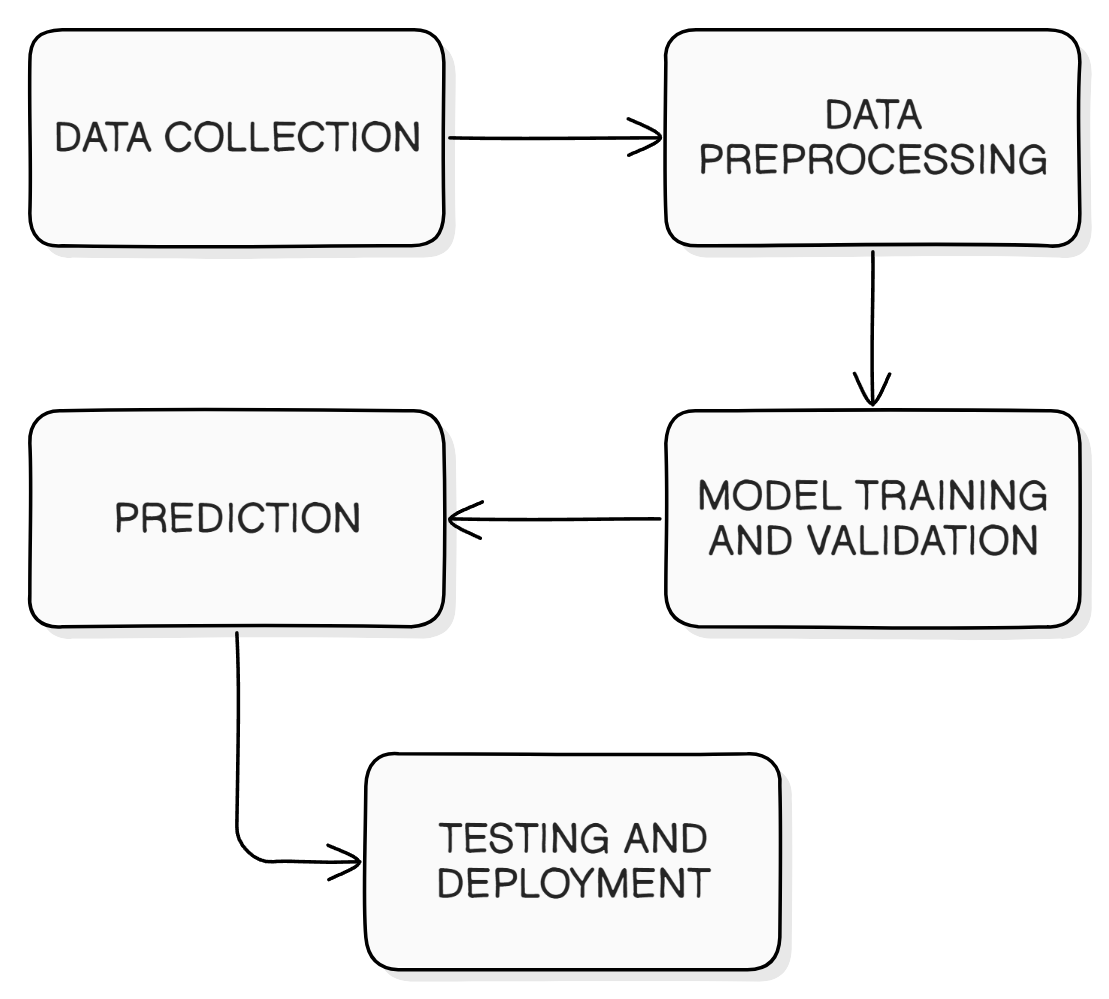
\includegraphics[width=0.5\textwidth]{Images/Project Modules.png}  
    \caption{Project Modules}
    \label{Project Modules}  % Label for referencing the figure
\end{figure}

\begin{table}[H]
    \centering
    \renewcommand{\arraystretch}{1.2} % Adjust row height for better readability
    \small % Reduce text size to fit within the page
    \begin{tabularx}{\textwidth}{|p{3.5cm}|X|}
        \hline
        \textbf{Module} & \textbf{Description} \\
        \hline
        \textbf{Data Collection} & Gathers relevant text data from posts in platforms like Reddit via PRAW. \\
        \hline
        \textbf{Data Preprocessing} & Cleans and prepares text data using:
        \begin{itemize}
            \setlength{\itemsep}{0pt}  % Adjust spacing between items
            \setlength{\parskip}{0pt}
            \item Tokenization (splitting text into words/tokens)
            \item Lowercasing for uniformity
            \item Stop-word removal
            \item Lemmatization or stemming
        \end{itemize} \\
        % \hline
        \textbf{} & Perform feature extraction to convert text into numerical features using:
        \begin{itemize}
            \setlength{\itemsep}{0pt}  % Adjust spacing between items
            \setlength{\parskip}{0pt}
            \item Term Frequency-Inverse Document Frequency (TF-IDF)
            \item Bag of Words (BoW) model
            \item Word2Vec, LIWC (Linguistic Inquiry and Word Count) and N-Gram were also explored
        \end{itemize} \\
        \hline
        \textbf{Model Training and Validation} & Splits dataset into training/testing sets and trains models such as:
        \setlength{\itemsep}{0pt}  % Adjust spacing between items
        \setlength{\parskip}{0pt}
        \begin{itemize}
            \item Logistic Regression, Naive Bayes, SVM, XGBoost, KNN, LSTM, Transformer. These formed the base models for the ensemble model used in application where Random Forest was used as the meta-learner All were validated to assess performance.
        \end{itemize} \\
        \hline
        \textbf{Prediction} & Processes received and combined text input for classification using trained models. \\
        \hline
        \textbf{Testing and} \newline \textbf{Deployment} & Deploys models on Streamlit Cloud for real-time predictions and wellbeing insights using association matrix. Provides a user interface for easy access. \\
        \hline
    \end{tabularx}
    \caption*{\textbf{Hierarchy of Modules in the system}}
    \label{tab:modules_hierarchy}
\end{table}


\subsection{Detailed Design}
% Provide hierarchy of modules or overall system diagram. 
% \vspace{.1in}
\begin{figure}[h!]  
    \centering
    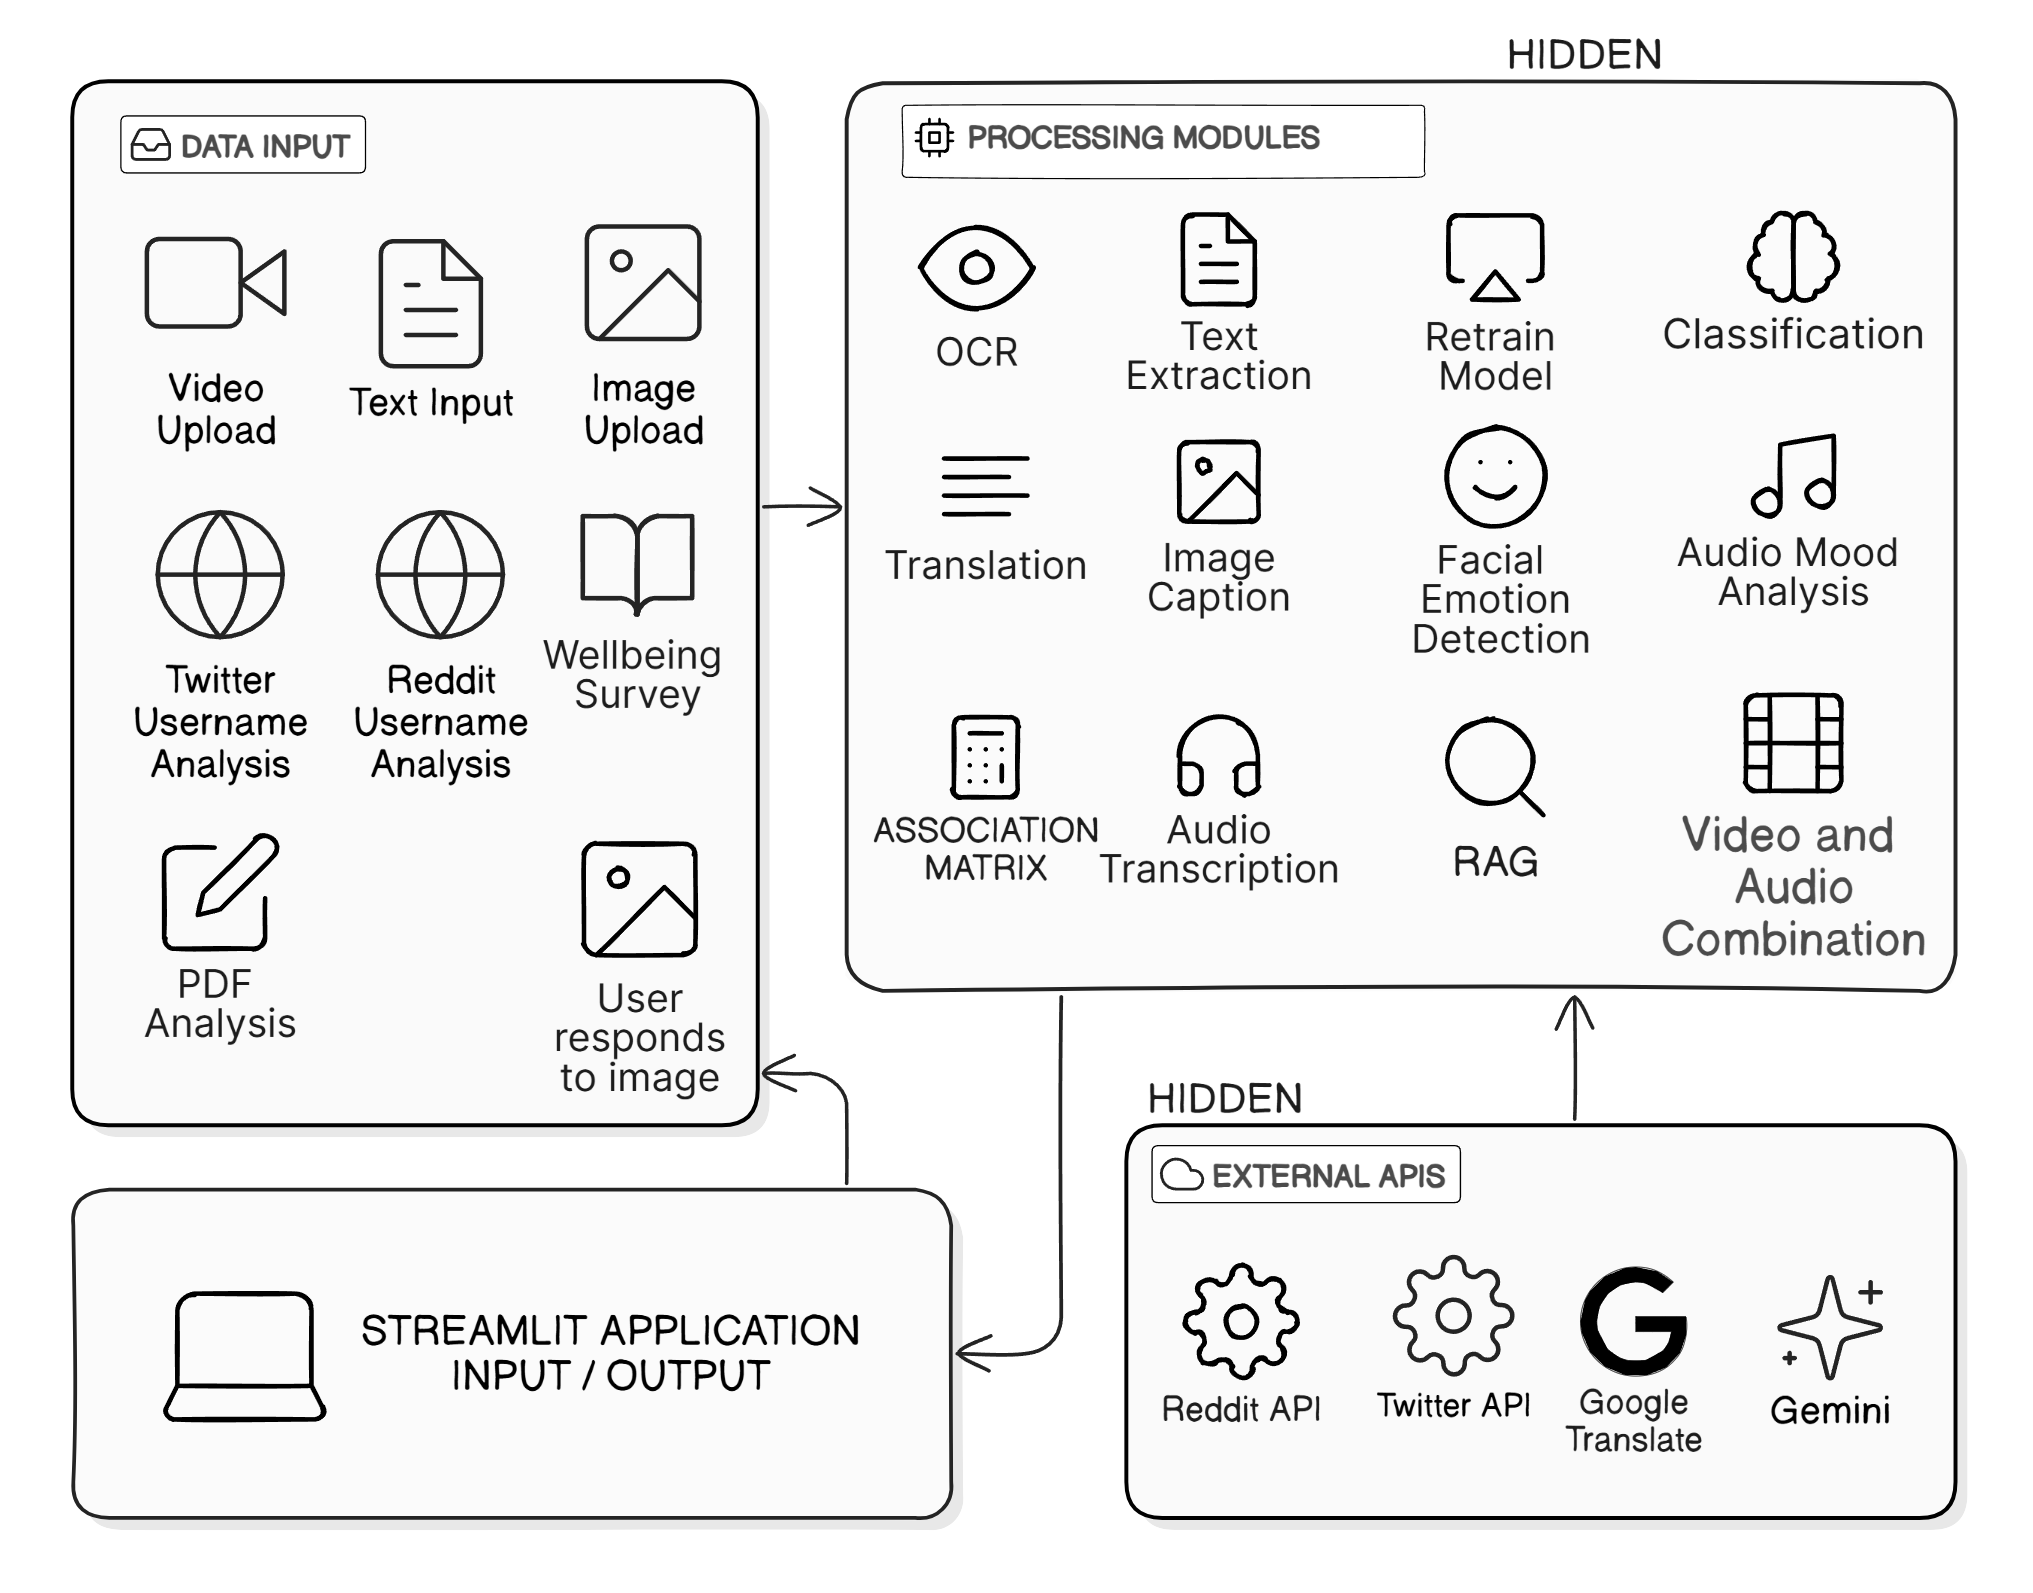
\includegraphics[width=0.85\textwidth]{Images/System Overview.png}  
    \caption{System Overview}
    \label{System Overview}  % Label for referencing the figure
\end{figure}

\begin{figure}[h!]  
    \centering
    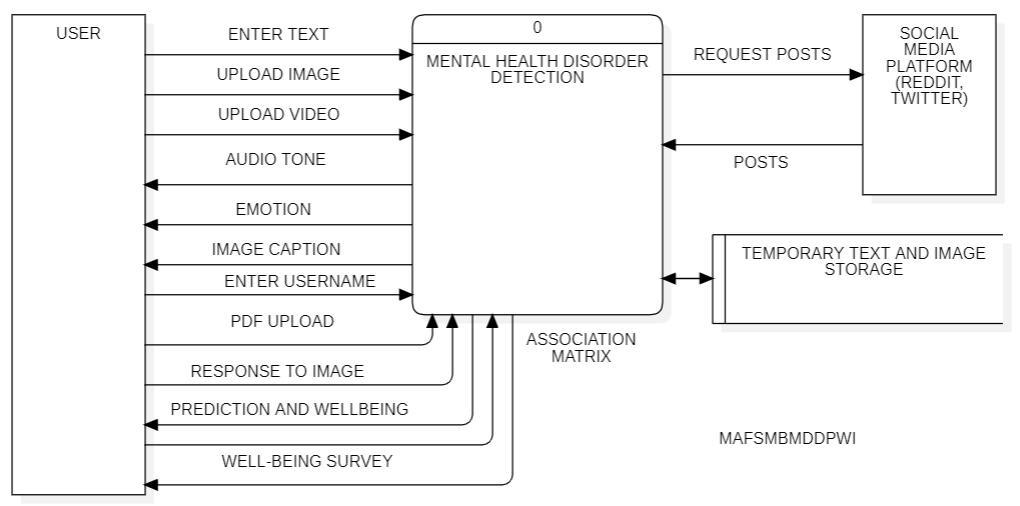
\includegraphics[width=0.85\textwidth]{Images/DFD L0.png}  
    \caption{DFD Level 0 of the System}
    \label{dfdl0123}  % Label for referencing the figure
\end{figure}

\pagebreak

\begin{figure}[h!]  
    \centering
    \includegraphics[width=0.725\textwidth]{Images/DFD L1.png}  
    \caption{DFD Level 1 of the System}
    \label{dfdl1234}  % Label for referencing the figure
\end{figure}

\vspace{2em}

\noindent
\textbf{Image Description}

\begin{figure}[h!]  
    \centering
    \includegraphics[width=0.7\textwidth]{Images/DFD L2 ID.png}  
    \caption{DFD Level 2 of Image Description}
    \label{dfdl122}  % Label for referencing the figure
\end{figure}

\noindent
The image captioning process using Python’s Transformers module and the ViT-GPT2 model involves several key steps. The user uploads an image, which is preprocessed by resizing to \(224 \times 224\) pixels, normalizing pixel values, and converting it into a tensor format. The Vision Transformer (ViT) divides the image into \(16 \times 16\) patches, embeds them, and processes them through transformer layers to extract visual features. The resulting embedding is passed to GPT-2, which generates a sequence of text tokens iteratively using its language model. Tokens are decoded back into human-readable text using the GPT-2 tokenizer, cleaned for readability, and output as a concise description. This pipeline leverages ViT for feature extraction and GPT-2 for language generation, enabling efficient and almost accurate image captioning.

\vspace{2em}

\noindent
\textbf{Emotion Detection Functionality}

\begin{figure}[h!]  
    \centering
    \includegraphics[width=0.7\textwidth]{Images/DFD L2 EMOTION.png}  
    \caption{DFD Level 2 of Emotion Detection Functionality}
    \label{dfdl14456}  % Label for referencing the figure
\end{figure}

\noindent
DeepFace analysis processes facial features from uploaded images or video frames through a structured pipeline. It starts with face detection using models like MTCNN, Dlib, or OpenCV to locate and align faces. The detected faces are cropped and passed to feature extraction, where pre-trained models like VGG-Face or Facenet generate numerical embeddings. These embeddings are compared using cosine similarity or Euclidean distance for tasks like emotion detection (e.g., happiness, sadness), demographic analysis (e.g., age, gender), or face verification. The results, such as detected emotions or attributes, are then displayed to the user. This process enables real-time analysis of facial expressions and emotions, providing valuable insights for mental health monitoring and wellbeing assessment.

\pagebreak

\noindent
\textbf{Extract Text From Image}

\begin{figure}[h!]  
    \centering
    \includegraphics[width=0.5\textwidth]{Images/DFD L2 TEXT EXTRACT.png}  
    \caption{DFD Level 2 of Text Extraction from Image}
    \label{dfdl13456}  % Label for referencing the figure
\end{figure}

\noindent
The process of extracting text from an image using Tesseract-OCR begins with preprocessing the uploaded image. The image is converted to grayscale, noise is reduced using Gaussian or Median Blur, and binarization (e.g., Otsu’s thresholding) isolates text from the background. Text regions are detected using contour analysis or connected components. The processed image is then passed to Tesseract, which uses an LSTM-based neural network to recognize characters and generate machine-readable text, enhanced by language models for accuracy. Postprocessing corrects errors via spell-checking and rule-based replacements (e.g., \texttt{0} $\rightarrow$ \texttt{O}), and formats the text into paragraphs or lines. The final output, displayed or saved as \texttt{.txt} or \texttt{.docx}, is ready for applications like document analysis. This pipeline combines image enhancement, deep learning, and text correction for high-quality results.

\vspace{2em}

\noindent
\textbf{Translation to English}

\begin{figure}[h!]  
    \centering
    \includegraphics[width=0.7\textwidth]{Images/DFD L2 TE.png}  
    \caption{DFD Level 2 of Translation to English}
    \label{dfdl111}  % Label for referencing the figure
\end{figure}

\noindent
The process of translating text to English using DeepTranslator begins with preprocessing the input to clean unwanted characters and detect the source language using machine learning models like Google’s Compact Language Detector. The prepared text is passed to DeepTranslator, which interfaces with APIs like Google Translate or Microsoft Translator. These APIs use neural machine translation (NMT) with encoder-decoder architectures and attention mechanisms to translate the text into English. Transformer-based models enhance accuracy by capturing context and long-range dependencies. Postprocessing ensures quality by validating completeness, correcting errors, and preserving formatting. The final translated text is displayed or saved, ensuring accuracy and readability. This pipeline integrates NLP, deep learning, and error handling for reliable translations.

\vspace{2em}

\noindent
\textbf{Audio Mood Analysis}

\begin{figure}[h!]  
    \centering
    \includegraphics[width=0.7\textwidth]{Images/DFD L2 AM.png}  
    \caption{DFD Level 2 of Audio Mood Analysis}
    \label{dfdl671}  % Label for referencing the figure
\end{figure}

\pagebreak

\noindent
The \texttt{analyze\_audio\_mood} function begins with the user providing a video file path. The audio is extracted using the \texttt{extract\_audio\_from\_video} function and loaded into memory with the Librosa library. Mel-frequency cepstral coefficients (MFCCs) are computed using \texttt{librosa.feature.mfcc} to capture frequency patterns for mood analysis. The MFCC array is segmented into four frequency bands—low, mid-low, mid-high, and high—and the scalar mean of each band is calculated to simplify data for classification. The mood is classified (e.g., normal, calm, anxious) based on the dominant frequency characteristics. Results can be further enhanced using the Gemini API to provide tone, mood, and summary details for the audio. This process combines audio feature extraction and classification for comprehensive mood analysis.

\vspace{2em}

\noindent
\textbf{Prediction to Wellbeing Mapping}

\begin{figure}[h!]  
    \centering
    \includegraphics[width=0.7\textwidth]{Images/DFD L2 MW.png}  
    \caption{DFD Level 2 of Prediction to Wellbeing Mapping}
    \label{dfdl166}  % Label for referencing the figure
\end{figure}

\noindent
The system first processes user input (text, behavioral data, or health metrics) through preprocessing and feature extraction. Machine learning models then predict the most likely mental health condition along with associated probabilities. The top predicted issue and its probability are then fed into GEMINI 2.0 FLASH with a structured prompt to generate wellbeing insights based on Ryff’s six parameters. To refine these insights, an association matrix maps the probabilities of all predicted issues to specific wellbeing parameters, selecting 1 to 3 key parameters (e.g., autonomy, personal growth, or self-acceptance). This ensures that the user receives targeted recommendations for improving their psychological wellbeing. There is also an additional feature where Retrieval Augmented Generation (RAG) is used to provide personalized recommendations based on the user’s mental health condition. The system retrieves relevant information from a knowledge base and generates tailored suggestions.
\vspace{1em}

\noindent
The above 6 main functionalities are reused in the application for the options available to the user. These include \textbf{Text} analysis, \textbf{Image} analysis, \textbf{Video} analysis, \textbf{PDF} analysis, analysis of \textbf{User response to Image}, analysis of \textbf{Reddit} and \textbf{Twitter} user profiles. \textbf{Wellbeing Survey Option} and \textbf{RAG for wellbeing Insights} have been added under \textit{Implementation} section.

\vspace{1em}

\noindent
Below are the flow diagrams for the various \textit{Analysis} options that the web application provides.

\begin{figure}[H]  
    \centering
    \includegraphics[width=0.72\textwidth]{Images/APP TEXT OPTION.png}  
    \caption{Text Classification Flow Diagram}
    \label{012i}  % Label for referencing the figure
\end{figure}

% -- pdf upload
\begin{figure}[H]  
    \centering
    \includegraphics[width=0.72\textwidth]{Images/APP PDF.png}  
    \caption{PDF Upload Flow Diagram}
    \label{01234i}  % Label for referencing the figure
\end{figure}

\pagebreak

\begin{figure}[H]  
    \centering
    \includegraphics[width=0.77\textwidth]{Images/APP IMAGE OPTION.png}  
    \caption{Image Classification Flow Diagram}
    \label{011232i}  % Label for referencing the figure
\end{figure}

% -- user response to image
\begin{figure}[H]  
    \centering
    \includegraphics[width=0.77\textwidth]{Images/APP RESPOND.png}  
    \caption{User Response to Image Flow Diagram}
    \label{01234i}  % Label for referencing the figure
\end{figure}

\pagebreak

\clearpage
\vspace*{\fill}
\vspace{-1cm}
\begin{figure}[H]
  \centering
  \includegraphics[width=\textwidth]{Images/APP VIDEO OPTION.png}
  \caption{Video Classification Flow Diagram}
  \label{01332i}
\end{figure}
\vspace*{\fill}
\clearpage

\pagebreak

\clearpage
\vspace*{\fill}
\vspace{-1cm}
\begin{figure}[H]  
    \centering
    \includegraphics[width=0.9\textwidth]{Images/APP REDDIT.png}  
    \caption{Reddit and Twitter username Classification Flow Diagram}
    \label{01234i}  % Label for referencing the figure
\end{figure}
\vspace*{\fill}
\clearpage

\pagebreak


% \noindent
% Create separate sections for separate modules of design as in Requirement Matrix. Ensure to provide Design Diagrams \textit{(e.g. System overview / DFDs / ERDs etc.; cross-reference to be drawn from Chapter 6), Decision matrix (for algorithm recommendation etc.) }




% \subsubsection{Name of Design Module 1 \label{sec:design_mod1}}
% \subsubsection{Name of Design Module 2 \label{sec:design_mod2}}
% \subsubsection{Name of Design Module 3 etc \label{sec:design_mod3}}


% Refer APPENDIX A  – Prototypes \ref{sec:proto} for prototype details.


% ------------------------------ Design Ends ---------------------------------


% --------------------------- Implementation ---------------------------------


\section{Implementation}
\subsection{Features From RM}
\noindent
For the initial prototype development, a subset of the requirements from the Requirement Matrix (RM) was carefully selected to focus on implementing core functionalities and demonstrating proof of concept. The selection was based on a combination of high-priority functional requirements that form the backbone of the system, ensuring that critical features are built and validated before expanding the scope. The requirements chosen for the prototype primarily involve data preprocessing, model training, and evaluation processes. These requirements were selected because they are fundamental to the project's success, ensuring that the data pipeline and model implementation work seamlessly together. This subset of features lays the groundwork for later integration with additional components and more complex functionality. The filtered part of the RM focuses on the following high-priority requirements: data cleaning and feature extraction, training of machine learning models, and evaluation of model performance using standard metrics. These requirements were identified as crucial because they directly impact the system's ability to handle data, learn patterns, and provide meaningful outputs. Without successfully implementing these core features, the overall effectiveness of the solution would be significantly reduced. Furthermore, these selected features align with the project’s goals and provide a clear pathway for incremental development. By narrowing down the requirements to these foundational aspects, the development team can ensure that the prototype is not only functional but also extensible, providing a robust framework for future enhancements.

\begin{figure}[h!]  
    \centering
    \includegraphics[width=0.7\textwidth]{Images/RM_part_for_implementation.png}  
    \caption{Features from Requirement Matrix}
    \label{Features from Requirement Matrix}  % Label for referencing the figure
\end{figure}

\begin{figure}[h!]  
    \centering
    \includegraphics[width=1.0\textwidth]{Images/ML Model Workflow.png}  
    \caption{Workflow for getting the model for the web application}
    \label{model workflow}  % Label for referencing the figure
\end{figure}


\subsection{Code Details and Output}

\subsubsection{Data Collection}

\begin{tcolorbox}[colback=gray!5!white, colframe=gray!80!black, boxrule=0.5pt, title=Collecting Reddit Posts]
    \begin{lstlisting}[language=Python]
import praw
import pandas as pd
import time
# Initialize Reddit API
reddit = praw.Reddit(client_id='YOUR_CLIENT_ID',
                        client_secret='YOUR_CLIENT_SECRET',
                        user_agent='Mental Health Classifier')
# Define subreddits and post types
subreddits = {'normal': ['news', 'AskReddit'], 
                'depression': ['depression'], 
                'ptsd': ['PTSD'], 
                'anxiety': ['Anxiety'], 
                'bipolar': ['BipolarReddit']}
post_types = ['hot', 'new', 'top']
posts_per_type = 100
# Collect and save posts
data = []
for label, subs in subreddits.items():
    for sub in subs:
        for post_type in post_types:
            posts = getattr(reddit.subreddit(sub), post_type)(limit=posts_per_type)
            for post in posts:
                data.append([post.title + " " + post.selftext, label])
            time.sleep(1)
df = pd.DataFrame(data, columns=['text', 'label'])
df.to_csv(f'{label}_dataset.csv', index=False)
    \end{lstlisting}
    \end{tcolorbox}
    
    \begin{figure}[h!]  
        \centering
        \includegraphics[width=0.9\textwidth]{Images/Dataset.png}  
        \caption{Obtained Dataset}
        \label{LSTMROC711}  % Label for referencing the figure
    \end{figure}


\begin{tcolorbox}[colback=gray!5!white, colframe=gray!80!black, boxrule=0.5pt, title=Combining Collected Datasets]
\begin{lstlisting}[language=Python]
import pandas as pd
from sklearn.utils import shuffle

# Load datasets
bipolar_df = pd.read_csv("bipolar_dataset.csv")
depression_df = pd.read_csv("depression_dataset.csv")
normal_df = pd.read_csv("normal_dataset.csv")
anxiety_df = pd.read_csv("anxiety_dataset.csv")
ptsd_df = pd.read_csv("ptsd_dataset.csv")

# Minimum length for balanced classes
min_length = min(len(bipolar_df), len(depression_df), len(normal_df) // 6, len(anxiety_df), len(ptsd_df))

# Create balanced pattern
pattern_data = []
for i in range(min_length):
    pattern_data.extend([bipolar_df.iloc[i], depression_df.iloc[i]] +
                        normal_df.iloc[i*6:(i+1)*6].to_dict('records') +
                        [anxiety_df.iloc[i], ptsd_df.iloc[i]])

pattern_df = pd.DataFrame(pattern_data)
remaining_data = shuffle(pd.concat([bipolar_df[min_length:], depression_df[min_length:], 
                                    normal_df[min_length*6:], anxiety_df[min_length:], ptsd_df[min_length:]]))

final_df = pd.concat([pattern_df, remaining_data]).reset_index(drop=True)
final_df.to_csv("mental_health_combined.csv", index=False)
\end{lstlisting}
\end{tcolorbox}
    
\noindent
The first code snippet collects Reddit posts by connecting to specific subreddits associated with various mental health topics. Using the Reddit API, posts are retrieved from `hot`, `new`, and `top` categories for each mental health type, including general subreddits (for the "normal" category). Each post’s title and content are combined, labeled, and saved into separate CSV files. The second code snippet merges these CSV files to form a combined dataset. It creates a balanced sample by selecting the minimum number of rows across each category and organizes the data in a structured pattern. Remaining rows are shuffled and appended, producing a final dataset suitable for machine learning applications in mental health classification.
    

% ----- adding subreddit info ------

\begin{figure}[h!]  
    \centering
    \includegraphics[width=1.0\textwidth]{Images/Data Collection Graph.png}  
    \caption{Collected Data Statistics}
    \label{LSTMROC7uyiut11}  % Label for referencing the figure
\end{figure}

\noindent
The dataset for mental health classification was compiled from various subreddit communities. Initially, the dataset contained records from 54 subreddits for anxiety, 38 for PTSD, 80 for depression, 60 for bipolar disorder, and 53 for normal mental states. Before data cleaning, the records totaled 38580 for anxiety, 34019 for PTSD, 36908 for depression, 30420 for bipolar, and 131725 for normal, reflecting the distribution of raw data. After applying data cleaning techniques to ensure quality and relevance, the record counts were reduced to 20456 for anxiety, 16386 for PTSD, 19446 for depression, 15746 for bipolar, and 95195 for normal. A subset of this cleaned dataset containing 18596 records was used for further processing and analysis.

\vspace{1em}

\noindent
Given the large size of the original dataset, training and testing the model on the entire dataset would require significant computational resources, including memory and processing power. Such constraints can lead to prolonged training times and potentially infeasible execution on standard hardware. By using a subset of the cleaned dataset, we can significantly reduce the computational load while maintaining a representative sample of the data. This approach strikes a balance between efficiency and performance, enabling the development and evaluation of models in a more manageable and resource-friendly manner. Moreover, working with a subset ensures faster experimentation and fine-tuning cycles, which is crucial for iterative improvement in machine learning workflows.

\pagebreak

\subsubsection{Data Preprocessing}

\begin{tcolorbox}[colback=gray!5!white, colframe=gray!80!black, boxrule=0.5pt, title=Text Preprocessing]
    \begin{lstlisting}[language=Python]
import pandas as pd
import re
from sklearn.feature_extraction.text import TfidfVectorizer
from nltk.corpus import stopwords
from nltk.tokenize import word_tokenize
import nltk

# Download stopwords (if you haven't already)
nltk.download('stopwords')
nltk.download('punkt')

# Load the dataset
df = pd.read_csv('mental_health.csv')

# 1. Handling Missing Values
df.dropna(subset=['text'], inplace=True)

# 2. Removing duplicates (if any)
df.drop_duplicates(subset=['text'], inplace=True)

# 3. Text Preprocessing
negative_words = {"not", "no", "nor", "never", "nothing", "nowhere", "neither", "cannot", "n't", "without", "barely", "hardly", "scarcely"}

def clean_text(text):
    text = re.sub(r'http\S+', '', text)  # Remove URLs
    text = re.sub(r'@\w+', '', text)  # Remove mentions (@username)
    text = re.sub(r'[^a-zA-Z\s]', '', text)  # Remove special characters, numbers, and punctuations
    text = text.lower()  # Convert text to lowercase
    tokens = word_tokenize(text)  # Tokenize the text
    tokens = [word for word in tokens if word not in stopwords.words('english') or word in negative_words]  # Remove stopwords, but keep negative words
    clean_text = ' '.join(tokens)  # Join the tokens back into a single string
    return clean_text

df['cleaned_text'] = df['text'].apply(clean_text)  # Apply the cleaning function to the 'text' column

\end{lstlisting}
\end{tcolorbox}

\begin{tcolorbox}[colback=gray!5!white, colframe=gray!80!black, boxrule=0.5pt, title=Text Preprocessing]
\begin{lstlisting}[language=Python]
# 4. Feature Extraction using TF-IDF Vectorization
vectorizer = TfidfVectorizer(max_features=10000)  # Adjust the max_features
X = vectorizer.fit_transform(df['cleaned_text'])  # Fit and transform the cleaned text data
X_df = pd.DataFrame(X.toarray(), columns=vectorizer.get_feature_names_out())  # Convert the result to a DataFrame for easier understanding

# Save the preprocessed dataset (optional)
df.to_csv('preprocessed_mental_health.csv', index=False)
    \end{lstlisting}
\end{tcolorbox}

\noindent
The code snippet above demonstrates the preprocessing steps for a mental health dataset. It handles missing values and duplicates in the text data, performs text cleaning by removing URLs, mentions, and special characters, and applies tokenization. The cleaned text is then vectorized using TF-IDF to convert the textual data into a format suitable for machine learning models. Finally, the preprocessed dataset is saved as a new CSV file for future use in classification tasks.

\begin{figure}[h!]  
    \centering
    \includegraphics[width=0.9\textwidth]{Images/Data Cleaning and Preprocessing.png}  
    \caption{Data Collection and Preprocessing}
    \label{Data Collection and Preprocessing}  % Label for referencing the figure
\end{figure}

% ------------ OTHER VECTORIZATIONS

\subsubsection{Vectorization Technqiues}

% Bag of Words
\begin{tcolorbox}[colback=gray!5!white, colframe=gray!80!black, boxrule=0.5pt, title=Bag of Words]
\begin{lstlisting}[language=Python]
from sklearn.feature_extraction.text import CountVectorizer

# Initialize the CountVectorizer and fit/transform the cleaned text
vectorizer = CountVectorizer()
X = vectorizer.fit_transform(dataset['cleaned_text'])
\end{lstlisting}
\end{tcolorbox}

\noindent
Bag of Words (BoW) converts text into a matrix of word counts. Each unique word in the corpus becomes a feature, and the value is the word's frequency in the document, ignoring grammar and word order.

% TF-IDF
\begin{tcolorbox}[colback=gray!5!white, colframe=gray!80!black, boxrule=0.5pt, title=TF-IDF]
\begin{lstlisting}[language=Python]
from sklearn.feature_extraction.text import TfidfVectorizer

# Initialize the TfidfVectorizer and fit/transform the cleaned text
TFIDFvectorizer = TfidfVectorizer()
X = TFIDFvectorizer.fit_transform(dataset['cleaned_text'])
\end{lstlisting}
\end{tcolorbox}

\noindent
Term Frequency-Inverse Document Frequency (TF-IDF) weighs words by their importance in a corpus. Common words receive lower weights, while rare words are assigned higher values, capturing their significance in the document.

% N-Gram
\begin{tcolorbox}[colback=gray!5!white, colframe=gray!80!black, boxrule=0.5pt, title=N-Gram]
\begin{lstlisting}[language=Python]
from sklearn.feature_extraction.text import CountVectorizer

# Initialize the CountVectorizer with n-grams (e.g., bi-grams and tri-grams)
vectorizer = CountVectorizer(ngram_range=(1, 3))
X = vectorizer.fit_transform(dataset['cleaned_text'])
\end{lstlisting}
\end{tcolorbox}
    
\noindent
N-Grams capture contiguous sequences of words to preserve some context. For example, bigrams (2-grams) capture pairs of words like "machine learning," and trigrams (3-grams) capture sequences like "natural language processing."

% LIWC
\begin{tcolorbox}[colback=gray!5!white, colframe=gray!80!black, boxrule=0.5pt, title=LIWC (Empath)]
\begin{lstlisting}[language=Python]
from empath import Empath

# Initialize Empath
lexicon = Empath()

# Function to get Empath features
def get_empath_features(text):
    analysis = lexicon.analyze(text, normalize=True)  # Normalize for proportions
    return analysis

# Generate Empath features for each text
empath_features = dataset['cleaned_text'].apply(get_empath_features)

# Convert Empath features to a DataFrame
X = pd.DataFrame(empath_features.tolist())
\end{lstlisting}
\end{tcolorbox}

\noindent
LIWC (Linguistic Inquiry and Word Count) analyzes text by categorizing words into meaningful psychological or social dimensions. Empath is a Python library that replicates this functionality with customizable lexicons. Empath is a Python-based natural language processing tool inspired by LIWC (Linguistic Inquiry and Word Count), designed to analyze text and categorize words into psychologically meaningful dimensions such as emotions, cognitive processes, and social themes. This tool is particularly valuable for extracting semantic features that capture the psychological and emotional aspects of textual data, making it ideal for applications in sentiment analysis, mental health studies, and psycholinguistics. By matching words in the text to predefined categories, Empath assigns a proportional representation to each category, indicating the relative frequency of words that belong to it. In the provided code, an \texttt{Empath} object is initialized, which serves as the base for analyzing text against the predefined lexicons. A function named \texttt{get\_empath\_features} is defined to process individual texts from the dataset. This function leverages the \texttt{analyze} method of the \texttt{Empath} object to compute the distribution of words across various categories. The \texttt{normalize=True} parameter ensures that the output represents proportions rather than raw counts, making the results more interpretable and comparable across texts of varying lengths. The function is applied to each piece of cleaned text in the dataset, producing a structured output where each text is represented as a dictionary. Each key in this dictionary corresponds to an Empath category, and the associated value indicates the proportion of words from the text that fall into that category. The list of dictionaries generated through this process is then converted into a DataFrame, where each column represents a category and each row corresponds to a document in the dataset. This transformation allows the extracted features to be seamlessly integrated into machine learning pipelines, where they can serve as predictors for tasks like sentiment analysis, mental health classification.

% Word2Vec
\begin{tcolorbox}[colback=gray!5!white, colframe=gray!80!black, boxrule=0.5pt, title=Word2Vec]
\begin{lstlisting}[language=Python]
from nltk.tokenize import word_tokenize
import gensim

# Tokenize the text data into words
def tokenize_text(text):
    return word_tokenize(text.lower())

dataset['tokens'] = dataset['cleaned_text'].apply(tokenize_text)

# Train a Word2Vec model using the tokenized data
word2vec_model = gensim.models.Word2Vec(sentences=dataset['tokens'], vector_size=100, window=5, min_count=1, workers=4)

# Function to average Word2Vec vectors for each document
def get_document_vector(tokens):
    valid_tokens = [word for word in tokens if word in word2vec_model.wv]
    if len(valid_tokens) == 0:
        return [0] * word2vec_model.vector_size  # Return zero vector for empty documents
    vectors = [word2vec_model.wv[word] for word in valid_tokens]
    return list(np.mean(vectors, axis=0))

# Convert the text data into document vectors
X = dataset['tokens'].apply(get_document_vector)
\end{lstlisting}
\end{tcolorbox}

\noindent
Word2Vec creates dense vector representations of words by training a neural network to predict words in context. These embeddings capture semantic meaning, and document vectors are computed by averaging word embeddings. The Python code implements a Word2Vec-based approach to transform text data into numerical vectors. First, the \texttt{tokenize\_text} function is defined to tokenize each text in the dataset into lowercase words, creating a new column named \texttt{tokens}. Using these tokenized sentences, a Word2Vec model is trained with parameters such as a vector size of 100, a context window of 5, and a minimum word frequency of 1. The \texttt{get\_document\_vector} function computes a document-level vector by averaging the Word2Vec embeddings of valid tokens in each text, ensuring that empty documents return a zero vector. Finally, the document vectors are calculated and stored in \texttt{X}, enabling their use as input features for downstream machine learning tasks.

\vspace{1em}

\noindent
The matrix dimensions for Bag of Words are determined by the number of records, which is 18,597 in this case, and the size of the vocabulary, which represents the number of unique words in the \texttt{cleaned\_text} column. Similarly, for TF-IDF, the dimensions of the matrix are the same as BOW, calculated as the number of records multiplied by the vocabulary size. For N-gram, the matrix size depends on the range of n-grams used. For example, a unigram produces dimensions equivalent to BOW, while bigram or trigram models increase the vocabulary size due to the inclusion of word combinations. Word2Vec, on the other hand, creates a dense vector representation for each word, with dimensions based on the predefined vector size, such as 100 or 200. Aggregating these vectors at the sentence level, typically by averaging, results in a matrix of dimensions equal to the number of records multiplied by the vector dimensions. For LIWC, the dimensions are determined by the number of predefined LIWC categories, which is typically around 70. The resulting matrix dimensions are the number of records multiplied by the number of LIWC categories.

% -------- logistic regression

\subsubsection{Logistic Regression Model for Classification}
\begin{tcolorbox}[colback=gray!5!white, colframe=gray!80!black, boxrule=0.5pt, title=Logistic Regression for Mental Health Classification]
    \begin{lstlisting}[language=Python]
import pandas as pd
from sklearn.model_selection import train_test_split
from sklearn.feature_extraction.text import CountVectorizer
from sklearn.linear_model import LogisticRegression
from sklearn.metrics import accuracy_score, classification_report, confusion_matrix

# Load the preprocessed dataset
dataset = pd.read_csv('preprocessed_mental_health.csv')
# Check if 'cleaned_text' and 'mental_health_issue' columns exist
if 'cleaned_text' not in dataset.columns or 'mental_health_issue' not in dataset.columns:
    raise ValueError("The dataset must have 'cleaned_text' and 'mental_health_issue' columns.")
# Remove rows with missing values in 'cleaned_text' column
dataset.dropna(subset=['cleaned_text'], inplace=True)
# Initialize the CountVectorizer and fit/transform the cleaned text
LRvectorizer = CountVectorizer()
X = LRvectorizer.fit_transform(dataset['cleaned_text'])
# Prepare the target variable
y = dataset['mental_health_issue']
\end{lstlisting}
\end{tcolorbox}

\begin{tcolorbox}[colback=gray!5!white, colframe=gray!80!black, boxrule=0.5pt, title=Logistic Regression for Mental Health Classification]
    \begin{lstlisting}[language=Python]
# Split the dataset into Training and Test Sets
X_train, X_test, y_train, y_test = train_test_split(X, y, test_size=0.2, random_state=42)
# Initialize the Logistic Regression model
LRmodel = LogisticRegression(multi_class='ovr', max_iter=10000)
# Train the model
LRmodel.fit(X_train, y_train)

# Make predictions on the test set
y_pred = LRmodel.predict(X_test)
# Evaluate the model
accuracy = accuracy_score(y_test, y_pred)
print(f'Accuracy: {accuracy * 100:.2f}%')

# Print classification report
print("Classification Report:\n", classification_report(y_test, y_pred))
# Print confusion matrix
print("Confusion Matrix:\n", confusion_matrix(y_test, y_pred))
\end{lstlisting}
\end{tcolorbox}

\noindent
The provided code demonstrates how to apply Logistic Regression for mental health classification using a preprocessed dataset. First, the dataset is loaded, and a check is performed to ensure that it contains the necessary columns, specifically \texttt{cleaned\_text} and \texttt{mental\_health\_issue}. If these columns are missing, an error is raised. The dataset is then cleaned by removing rows that have missing values in the \texttt{cleaned\_text} column using the \texttt{dropna()} function. Next, the \texttt{CountVectorizer} is initialized and applied to the \texttt{cleaned\_text} column to convert the text data into a numerical format suitable for machine learning. This is accomplished by transforming the text into a document-term matrix where each row represents a document (post) and each column represents a unique term (word). The target variable, \texttt{mental\_health\_issue}, is also extracted from the dataset.The dataset is then split into training and testing sets using \texttt{train\_test\_split()}, where 80\% of the data is used for training, and 20\% is reserved for testing. The \texttt{random\_state} is set to ensure reproducibility of the results. A Logistic Regression model is initialized with a multi-class strategy (\texttt{multi\_class='ovr'}) and a high number of iterations (\texttt{max\_iter=10000}) to allow the model to converge. The model is then trained on the training data using the \texttt{fit()} method. After training, predictions are made on the test set using the \texttt{predict()} method. The model's performance is evaluated by calculating the accuracy score, which is printed as a percentage. Additionally, a detailed classification report is generated, which includes metrics such as precision, recall, and F1-score for each class. Lastly, a confusion matrix is printed to visualize the model's classification performance and to understand how well the model distinguishes between different mental health issues. This end-to-end pipeline is crucial for applying Logistic Regression to textual data, allowing for effective classification of mental health issues based on Reddit posts.

% ----------- naive bayes

\subsubsection{Naive Bayes for Classification}

\begin{tcolorbox}[colback=gray!5!white, colframe=gray!80!black, boxrule=0.5pt, title=Naive Bayes for Mental Health Classification]
    \begin{lstlisting}[language=Python]
# KEEPING THE EXACT SAME IMPLEMENTATION CODE AS THE LOGISTIC REGRESSION

# Initialize the Naive Bayes classifier
NBmodel = MultinomialNB()
# Fit the model
NBmodel.fit(X_train, y_train)
# Make predictions
y_pred = NBmodel.predict(X_test)

    \end{lstlisting}
\end{tcolorbox}

\noindent
The provided code applies the Naive Bayes classifier (MultinomialNB) for mental health classification using a preprocessed dataset. A Naive Bayes model (\texttt{MultinomialNB}) is initialized and trained on the training data using the \texttt{fit()} method. After training, predictions are made on the test set using the \texttt{predict()} method.

% --------- svc

\subsubsection{Support Vector Machine for Classification}

\begin{tcolorbox}[colback=gray!5!white, colframe=gray!80!black, boxrule=0.5pt, title=Support Vector Classifier Implementation]
    \begin{lstlisting}[language=Python]
# KEEPING THE EXACT SAME IMPLEMENTATION CODE AS THE LOGISTIC REGRESSION

# Initialize the Support Vector Classifier
SVMmodel = SVC(kernel='linear', C=1, random_state=42, probability=True)  # You can adjust parameters as needed

# Train the model
SVMmodel.fit(X_train, y_train)
# Make predictions on the test set
y_pred = SVMmodel.predict(X_test)
\end{lstlisting}
\end{tcolorbox}

\noindent
 A Support Vector Classifier model (\texttt{SVC}) is initialized with a linear kernel (\texttt{kernel='linear'}), regularization parameter \texttt{C=1}, and the probability flag set to \texttt{True} to enable probability estimates. The model is then trained on the training data using the \texttt{fit()} method. After training, predictions are made on the test set using the \texttt{predict()} method. 

% ----------------- random forest

\subsubsection{Random Forest for Classification}
  
\begin{tcolorbox}[colback=gray!5!white, colframe=gray!80!black, boxrule=0.5pt, title=Random Forest Classifier Implementation]
    \begin{lstlisting}[language=Python]
# KEEPING THE EXACT SAME IMPLEMENTATION CODE AS THE LOGISTIC REGRESSION

# Initialize the Random Forest Classifier with added parameters
RFmodel = RandomForestClassifier(n_estimators=3000, max_depth=None, min_samples_split=20, min_samples_leaf=1, max_features='sqrt', bootstrap=False, random_state=42)

# Train the model
RFmodel.fit(X_train, y_train)
# Make predictions on the test set
y_pred = RFmodel.predict(X_test)
    \end{lstlisting}
\end{tcolorbox}

\noindent
 A Random Forest Classifier model is initialized with several hyperparameters. Specifically, \texttt{n\_estimators=3000} defines the number of decision trees in the forest. The \texttt{max\_depth=None} means the trees are allowed to grow until all leaves are pure or contain fewer than the minimum samples required to split a node. The \texttt{min\_samples\_split=20} and \texttt{min\_samples\_leaf=1} specify the minimum number of samples required to split an internal node and the minimum number of samples required to be at a leaf node, respectively. The \texttt{max\_features='sqrt'} sets the maximum number of features to consider for the best split at each node to be the square root of the total number of features. \texttt{bootstrap=False} disables bootstrapping, meaning the entire dataset is used to build each tree. After initialization, the model is trained using the \texttt{fit()} method on the training data. After training, predictions are made on the test set using the \texttt{predict()} method.


% ----------- xgboost

\subsubsection{XGBoost for Classification}

\begin{tcolorbox}[colback=gray!5!white, colframe=gray!80!black, boxrule=0.5pt, title=XGBoost Classifier Implementation]
    \begin{lstlisting}[language=Python]
# WITH THE EXACT SAME IMPLEMENTATION CODE. THE CountVectorizer IS CHANGED TO TF-IDF

# Convert text data to numerical data using TF-IDF Vectorizer
from sklearn.feature_extraction.text import TfidfVectorizer
tfidf = TfidfVectorizer(max_features=5000)
X_train = tfidf.fit_transform(X_train)
X_test = tfidf.transform(X_test)
\end{lstlisting}
\end{tcolorbox}
\begin{tcolorbox}[colback=gray!5!white, colframe=gray!80!black, boxrule=0.5pt, title=XGBoost Classifier Implementation]
    \begin{lstlisting}[language=Python]
# Define the XGBoost classifier
xgb_clf = xgb.XGBClassifier(objective='multi:softmax', num_class=5, eval_metric='mlogloss', use_label_encoder=False)

# Train the model
xgb_clf.fit(X_train, y_train)
# Predict on the test set
y_pred = xgb_clf.predict(X_test)
\end{lstlisting}
\end{tcolorbox}

\noindent
The text data is transformed into numerical features using the \texttt{TfidfVectorizer()}. This vectorizer converts the raw text into a matrix of TF-IDF (Term Frequency-Inverse Document Frequency) features, which are more suitable for training a machine learning model. The \texttt{max\_features=5000} parameter limits the number of features to the 5000 most frequent terms in the dataset. The XGBoost classifier is then initialized with several hyperparameters. The \texttt{objective='multi:softmax'} indicates that the task is a multi-class classification problem. The \texttt{num\_class=5} parameter specifies the number of classes for the classification task, and \texttt{eval\_metric='mlogloss'} is set to use the log loss metric for evaluation. \texttt{use\_label\_encoder=False} disables the automatic label encoding of target labels, as we have already manually encoded the labels. After initialization, the model is trained on the training data using the \texttt{fit()} method. 

% ------------ knn

\subsubsection{K Nearest Neighbours for Classification}

\begin{tcolorbox}[colback=gray!5!white, colframe=gray!80!black, boxrule=0.5pt, title=k-NN Classifier Implementation for Mental Health Classification]
    \begin{lstlisting}[language=Python]
# KEEPING THE EXACT SAME IMPLEMENTATION CODE AS THE LOGISTIC REGRESSION 

# Initialize the k-NN classifier
KNNmodel = KNeighborsClassifier(n_neighbors=5)  
# Fit the model
KNNmodel.fit(X_train, y_train)
# Make predictions
y_pred = KNNmodel.predict(X_test)
\end{lstlisting}
\end{tcolorbox}

\noindent
 A k-NN classifier is initialized with 5 neighbors (\texttt{n\_neighbors=5}), though this number can be adjusted for tuning the model. The classifier is trained on the training data using the \texttt{fit()} method. Once the model is trained, it is used to predict mental health issues for the test set, and the accuracy of the predictions is calculated and printed. 

% --------------- lstm

\subsubsection{Long Short Term Memory based Classification}

\begin{tcolorbox}[colback=gray!5!white, colframe=gray!80!black, boxrule=0.5pt, title=LSTM Model Implementation]
    \begin{lstlisting}[language=Python]
import pandas as pd
import numpy as np
import matplotlib.pyplot as plt
import seaborn as sns
from sklearn.metrics import confusion_matrix, classification_report
from sklearn.preprocessing import LabelEncoder
from tensorflow.keras.preprocessing.text import Tokenizer
from tensorflow.keras.preprocessing.sequence import pad_sequences
from tensorflow.keras.models import Sequential
from tensorflow.keras.layers import Embedding, LSTM, Dense, Dropout
from tensorflow.keras.utils import to_categorical
from sklearn.model_selection import train_test_split

# Load the dataset
data = pd.read_csv('preprocessed_mental_health.csv')
# Separate features and target
X = data['text']
y = data['mental_health_issue']
# Encode target labels
label_encoder = LabelEncoder()
y = label_encoder.fit_transform(y)
y = to_categorical(y)  # Convert labels to one-hot encoded format for multi-class classification
# Split dataset into training and test sets
X_train, X_test, y_train, y_test = train_test_split(X, y, test_size=0.2, random_state=42)
# Tokenize and pad the text sequences
vocab_size = 10000  # Set a vocabulary size
max_length = 100    # Set a max length for padding

tokenizer = Tokenizer(num_words=vocab_size, oov_token="<OOV>")
tokenizer.fit_on_texts(X_train)
X_train_seq = tokenizer.texts_to_sequences(X_train)
X_test_seq = tokenizer.texts_to_sequences(X_test)
X_train_padded = pad_sequences(X_train_seq, maxlen=max_length, padding='post', truncating='post')
\end{lstlisting}
\end{tcolorbox}

\begin{tcolorbox}[colback=gray!5!white, colframe=gray!80!black, boxrule=0.5pt, title=LSTM Model Implementation]
    \begin{lstlisting}[language=Python]
X_test_padded = pad_sequences(X_test_seq, maxlen=max_length, padding='post', truncating='post')
# Build the LSTM model
model = Sequential([ Embedding(vocab_size, 128, input_length=max_length), LSTM(128,eturn_sequences=True), Dropout(0.2), LSTM(64), Dropout(0.2), Dense(64,activation='relu'), Dense(y.shape[1],activation='softmax')])

model.compile(optimizer='adam', loss='categorical_crossentropy', metrics=['accuracy'])
# Train the model
history = model.fit(X_train_padded, y_train, epochs=10, batch_size=32, validation_data=(X_test_padded, y_test))

# Evaluate the model on test data
test_loss, test_accuracy = model.evaluate(X_test_padded, y_test)
print(f"Test Accuracy: {test_accuracy * 100:.2f}%")
# Generate predictions and convert back from one-hot encoding
y_pred = model.predict(X_test_padded)
y_pred_classes = np.argmax(y_pred, axis=1)
y_test_classes = np.argmax(y_test, axis=1)
\end{lstlisting}
\end{tcolorbox}

\noindent
This code demonstrates how to apply a Long Short-Term Memory (LSTM) neural network for text classification, specifically for predicting mental health issues based on preprocessed Reddit data. The dataset is loaded and the target variable (\texttt{mental\_health\_issue}) is encoded into a one-hot format for multi-class classification. The dataset is split into training and testing sets. Text data is tokenized and padded to ensure uniform input lengths for the LSTM model. The model consists of embedding layers, LSTM layers with dropout for regularization, and dense layers for classification. The model is trained on the training data, and performance is monitored using validation data. The training and validation accuracy and loss are plotted. The model is evaluated on the test data, and performance metrics such as accuracy and classification report are displayed. A confusion matrix is plotted to visualize model performance.

\begin{figure}[h!]  
    \centering
    \includegraphics[width=0.8\textwidth]{Images/LSTM Epoch.png}  
    \caption{Output for LSTM Epochs}
    \label{LSTm Epochs}  % Label for referencing the figure
\end{figure}

\begin{figure}[h!]  
    \centering
    \includegraphics[width=0.8\textwidth]{Images/LSTM LA.png}  
    \caption{LSTM Validation loss and accuracy}
    \label{Accuracy Loss}  % Label for referencing the figure
\end{figure}

\begin{figure}[h!]  
    \centering
    \includegraphics[width=0.8\textwidth]{Images/LSTM EMBED.png}  
    \caption{LSTM Random and Learned Embeddings}
    \label{lstm embed}  % Label for referencing the figure
\end{figure}

\begin{figure}[h!]  
    \centering
    \includegraphics[width=0.45\textwidth]{Images/LSTM MODEL.png}  
    \caption{LSTM Model Architecture}
    \label{lstm arch}  % Label for referencing the figure
\end{figure}

% ---------- hyperparameter tuning

\subsubsection{Hyperparamter Tuning Using RandomizedSearchCV}

\begin{tcolorbox}[colback=gray!5!white, colframe=gray!80!black, boxrule=0.5pt, title=Logistic Regression]
\begin{lstlisting}[language=Python]
import pandas as pd
from sklearn.model_selection import train_test_split, RandomizedSearchCV
from sklearn.feature_extraction.text import CountVectorizer
from sklearn.linear_model import LogisticRegression
from sklearn.metrics import accuracy_score, classification_report

# Load the preprocessed dataset
dataset = pd.read_csv('preprocessed_mental_health.csv')
if 'cleaned_text' not in dataset.columns or 'mental_health_issue' not in dataset.columns:
    raise ValueError("The dataset must have 'cleaned_text' and 'mental_health_issue' columns.")
\end{lstlisting}
\end{tcolorbox}

\begin{tcolorbox}[colback=gray!5!white, colframe=gray!80!black, boxrule=0.5pt, title=Logistic Regression]
    \begin{lstlisting}[language=Python]
# Remove rows with missing values in 'cleaned_text' column
dataset.dropna(subset=['cleaned_text'], inplace=True)

# Initialize the CountVectorizer and fit/transform the cleaned text
HPLRvectorizer = CountVectorizer()
X = HPLRvectorizer.fit_transform(dataset['cleaned_text'])

# Prepare the target variable
y = dataset['mental_health_issue']
# Split the dataset into Training and Test Sets
X_train, X_test, y_train, y_test = train_test_split(X, y, test_size=0.2, random_state=42)

# Initialize the Logistic Regression model
HPLRmodel = LogisticRegression(max_iter=200)
# Define the hyperparameter grid for Randomized Search
param_distributions = {
    'C': [0.001, 0.01, 0.1, 1, 10, 100], 'penalty': ['l1', 'l2', 'elasticnet', 'none'], 'solver': ['liblinear', 'saga']}

# Initialize RandomizedSearchCV
random_search = RandomizedSearchCV(estimator=HPLRmodel, param_distributions=param_distributions, n_iter=10, scoring='accuracy', cv=5, n_jobs=-1, random_state=42)

random_search.fit(X_train, y_train)
print("Best Hyperparameters:", random_search.best_params_)
best_modelLR = random_search.best_estimator_
y_pred = best_modelLR.predict(X_test)

# Evaluate the model
accuracy = accuracy_score(y_test, y_pred)
print(f'Accuracy: {accuracy * 100:.2f}%')
# Print classification report
print("Classification Report:\n", classification_report(y_test, y_pred))
\end{lstlisting}
\end{tcolorbox}

\noindent
The above code demonstrates a machine learning workflow for classifying mental health issues using \texttt{LogisticRegression} with hyperparameter tuning. The dataset is loaded using \texttt{pandas}, and a check ensures the presence of \texttt{'cleaned\_text'} and \texttt{'mental\_health\_issue'} columns. Missing values in \texttt{'cleaned\_text'} are dropped to prevent processing errors. The textual data is transformed into a numerical format using \texttt{CountVectorizer}, which converts text into a bag-of-words representation. The dataset is then split into training and testing sets using \texttt{train\_test\_split}. A logistic regression model is initialized, and the hyperparameter grid is defined, including parameters like \texttt{C} (inverse of regularization strength), \texttt{penalty}, and \texttt{solver}. Hyperparameter tuning is performed using \texttt{RandomizedSearchCV}, which searches for the best model configuration by sampling parameter combinations. The best model is used to make predictions on the test set, and evaluation metrics such as accuracy and a classification report are printed.


\begin{tcolorbox}[colback=gray!5!white, colframe=gray!80!black, boxrule=0.5pt, title=K Nearest Neighbours]
    \begin{lstlisting}[language=Python]
# KEEPING THE EXACT SAME IMPLEMENTATION CODE AS THE Hyperparameter Tuning ON LOGISTIC REGRESSION

# Initialize the k-NN classifier
knn = KNeighborsClassifier()

# Define the hyperparameter grid for Randomized Search
param_distributions = {
    'n_neighbors': [3, 4, 5, 6, 7, 8, 9, 10, 11, 12, 13, 15, 14, 15, 16, 17, 18, 19, 20],
        # Different values for number of neighbors
    'metric': ['euclidean', 'manhattan', 'chebyshev', 'minkowski'],  # Different distance metrics
    'weights': ['uniform', 'distance']  # Weighing options for neighbors
}

# Initialize RandomizedSearchCV
random_search = RandomizedSearchCV(estimator=knn, param_distributions=param_distributions,
                                    n_iter=10, scoring='accuracy', cv=5, n_jobs=-1, random_state=42)

# Fit RandomizedSearchCV
random_search.fit(X_train, y_train)
# Best hyperparameters from Random Search
print("Best Hyperparameters:", random_search.best_params_)
# Best model from Random Search
best_knn = random_search.best_estimator_
# Make predictions using the best model
y_pred = best_knn.predict(X_test)
\end{lstlisting}
\end{tcolorbox}

\noindent
The k-NN model is initialized without predefined parameters, and a hyperparameter grid is defined for tuning. This grid explores various values for the number of neighbors (\texttt{n\_neighbors}), distance metrics (\texttt{metric}), and neighbor weighting options (\texttt{weights}). \texttt{RandomizedSearchCV} is then used to optimize these parameters by training multiple k-NN models with combinations from the grid, evaluating them with 5-fold cross-validation, and scoring based on accuracy. The best combination of hyperparameters is identified and used to configure the final k-NN model.


\begin{tcolorbox}[colback=gray!5!white, colframe=gray!80!black, boxrule=0.5pt, title=Support Vector Machine]
    \begin{lstlisting}[language=Python]
# KEEPING THE EXACT SAME IMPLEMENTATION CODE AS THE Hyperparameter Tuning ON LOGISTIC REGRESSION

# Initialize the SVC model
model = SVC()

# Define the hyperparameter grid for Randomized Search
param_distributions = {
    'C': [0.1, 1, 10, 100],               # Regularization parameter
    'kernel': ['linear', 'rbf', 'poly'],  # Kernel types
    'gamma': ['scale', 'auto', 0.1, 1],   # Kernel coefficient for 'rbf', 'poly', and 'sigmoid'
}

# Initialize RandomizedSearchCV
random_search = RandomizedSearchCV(estimator=model, param_distributions=param_distributions,
                                    n_iter=10, scoring='accuracy', cv=5, n_jobs=-1, random_state=42)

# Fit RandomizedSearchCV
random_search.fit(X_train, y_train)
# Best hyperparameters from Random Search
print("Best Hyperparameters:", random_search.best_params_)
# Best model from Random Search
best_model = random_search.best_estimator_
# Make predictions using the best model
y_pred = best_model.predict(X_test)
\end{lstlisting}
\end{tcolorbox}

\noindent
The SVC model is initialized without predefined hyperparameters, and a hyperparameter grid is defined for tuning. This grid includes different values for the regularization parameter (\texttt{C}), kernel types (\texttt{kernel}), and the kernel coefficient (\texttt{gamma}). \texttt{RandomizedSearchCV} is employed to find the best combination of these parameters by evaluating multiple models with various hyperparameter combinations through 5-fold cross-validation, using accuracy as the scoring metric. The best set of hyperparameters is selected to configure the final SVC model. 

\begin{tcolorbox}[colback=gray!5!white, colframe=gray!80!black, boxrule=0.5pt, title=Naive Bayes]
    \begin{lstlisting}[language=Python]
# KEEPING THE EXACT SAME IMPLEMENTATION CODE AS THE Hyperparameter Tuning ON LOGISTIC REGRESSION

# Initialize the Naive Bayes model
naive_bayes_model = MultinomialNB()

# Define the parameter distribution for Randomized Search
param_distributions = {
    'alpha': uniform(0.001, 5.0)  # Sampling alpha from a uniform distribution
}

# Initialize RandomizedSearchCV
random_search = RandomizedSearchCV(estimator=naive_bayes_model, param_distributions=param_distributions,
                                    n_iter=10, scoring='accuracy', cv=5, n_jobs=-1, random_state=42)

# Fit RandomizedSearchCV
random_search.fit(X_train, y_train)
# Best hyperparameters from Random Search
print("Best Hyperparameters:", random_search.best_params_)
# Best model from Random Search
best_model = random_search.best_estimator_
# Make predictions using the best model
y_pred = best_model.predict(X_test)
    \end{lstlisting}
\end{tcolorbox}

\noindent
 The Naive Bayes model is initialized, and a parameter distribution for \texttt{alpha} is defined using a uniform distribution, sampling values between 0.001 and 5.0. \texttt{RandomizedSearchCV} is utilized to explore different values for \texttt{alpha} over 10 iterations, using 5-fold cross-validation and accuracy as the scoring metric. The best hyperparameters are identified and used to configure the final Naive Bayes model. The model is then tested on the unseen data (test set).

% ---------- transformer -------
\subsubsection{Tranformer based model for classification}

\begin{tcolorbox}[colback=gray!5!white, colframe=gray!80!black, boxrule=0.5pt, title=Importing Libraries]
    \begin{lstlisting}[language=Python]
import numpy as np
import pandas as pd
from sklearn.preprocessing import LabelEncoder
from sklearn.metrics import confusion_matrix, ConfusionMatrixDisplay
from tensorflow.keras.layers import MultiHeadAttention, Input, Dense, Embedding, GlobalAveragePooling1D, LayerNormalization, Layer
from tensorflow.keras.models import Model, Sequential
from tensorflow.keras.utils import to_categorical
from tensorflow.keras.layers import TextVectorization
import matplotlib.pyplot as plt
from tensorflow.data import Dataset
from tensorflow import convert_to_tensor, string, float32, shape, range, reshape
    \end{lstlisting}
\end{tcolorbox}

\noindent
The provided Python code imports a set of essential libraries and modules used for data processing, machine learning, and neural network construction. NumPy and pandas are used for numerical computations and data manipulation, while scikit-learn provides tools like label encoding and confusion matrix evaluation. TensorFlow modules enable the construction of advanced deep learning architectures with layers such as multi-head attention and embeddings, alongside utilities for text vectorization and categorical encoding. Matplotlib is utilized for visualizations, and TensorFlow's Dataset API facilitates efficient data handling and pipeline creation for training models.

\begin{tcolorbox}[colback=gray!5!white, colframe=gray!80!black, boxrule=0.5pt, title=Load Dataset]
    \begin{lstlisting}[language=Python]
from google.colab import files

# Upload the file
uploaded = files.upload()
# Load dataset
file_path = 'preprocessed_mental_health.csv'
data = pd.read_csv(file_path)

# Drop rows with missing cleaned_text
data = data.dropna(subset=['cleaned_text'])
# Extract features and labels
texts = data['cleaned_text'].astype(str).values
labels = data['mental_health_issue'].astype(str).values
    \end{lstlisting}
\end{tcolorbox}

\noindent
This code snippet uses Google Colab's `files` module to upload datasets interactively, enabling easy integration with cloud-based environments. It then loads a dataset in CSV format using pandas and preprocesses the data by dropping rows with missing values in the `cleaned\_text` column. The `cleaned\_text` column is used to extract the textual features, and the `mental\_health\_issue` column provides the corresponding labels for classification tasks, both stored as NumPy arrays.

\begin{tcolorbox}[colback=gray!5!white, colframe=gray!80!black, boxrule=0.5pt, title=Processing Labels and Text Vectorization]
    \begin{lstlisting}[language=Python]
# Encode the labels
label_encoder = LabelEncoder()
encoded_labels = label_encoder.fit_transform(labels)
categorical_labels = to_categorical(encoded_labels)

# Get class names
class_names = label_encoder.classes_
print("Classes:", class_names)
# Define parameters
vocab_size = 25000
sequence_length = 300

# Vectorization layer
vectorize_layer = TextVectorization(max_tokens=vocab_size, output_sequence_length=sequence_length)

# Adapt vectorizer to texts
vectorize_layer.adapt(Dataset.from_tensor_slices(texts))
# Vectorize text data
texts_vectorized = vectorize_layer(convert_to_tensor(texts, dtype=string))
    \end{lstlisting}
\end{tcolorbox}

This code snippet encodes textual labels into numerical format using the `LabelEncoder` from scikit-learn and transforms them into categorical labels suitable for deep learning models. The class names are retrieved and displayed for reference. A `TextVectorization` layer is defined with specified vocabulary size and sequence length to preprocess text data into numerical format. The vectorization layer is adapted to the text dataset, and the texts are vectorized into fixed-length sequences for model input.

\begin{tcolorbox}[colback=gray!5!white, colframe=gray!80!black, boxrule=0.5pt, title=Define Transformer Model]
    \begin{lstlisting}[language=Python]
class EmbeddingLayer(Layer):
    def __init__(self, sequence_length, vocab_size, embed_dim):
        super(EmbeddingLayer, self).__init__()
        self.word_embedding = Embedding(input_dim=vocab_size, output_dim=embed_dim)
        self.position_embedding = Embedding(input_dim=sequence_length, output_dim=embed_dim)

    def call(self, tokens):
        sequence_length = shape(tokens)[-1]
        positions = range(start=0, limit=sequence_length, delta=1)
        positions_encoding = self.position_embedding(positions)
        words_encoding = self.word_embedding(tokens)
        return positions_encoding + words_encoding

class EncoderLayer(Layer):
    def __init__(self, total_heads, total_dense_units, embed_dim):
        super(EncoderLayer, self).__init__()
        self.multihead = MultiHeadAttention(num_heads=total_heads, key_dim=embed_dim)
        self.nnw = Sequential([Dense(total_dense_units, activation="relu"), Dense(embed_dim)])
        self.normalize_layer = LayerNormalization()

    def call(self, inputs):
        attn_output = self.multihead(inputs, inputs)
        normalize_attn = self.normalize_layer(inputs + attn_output)
        nnw_output = self.nnw(normalize_attn)
        final_output = self.normalize_layer(normalize_attn + nnw_output)
        return final_output

# Model parameters
embed_dim = 64
num_heads = 2
total_dense_units = 60

# Define the model
inputs = Input(shape=(sequence_length,))
embedding_layer = EmbeddingLayer(sequence_length, vocab_size, embed_dim)
encoder_layer = EncoderLayer(num_heads, total_dense_units, embed_dim)
\end{lstlisting}
\end{tcolorbox}
\begin{tcolorbox}[colback=gray!5!white, colframe=gray!80!black, boxrule=0.5pt, title=Define Transformer Model]
    \begin{lstlisting}[language=Python]
emb = embedding_layer(inputs)
enc = encoder_layer(emb)
pool = GlobalAveragePooling1D()(enc)
dense = Dense(total_dense_units, activation="relu")(pool)
outputs = Dense(len(class_names), activation="softmax")(dense)

transformer_model = Model(inputs=inputs, outputs=outputs)
transformer_model.compile(optimizer="adamw", loss="categorical_crossentropy", metrics=['accuracy'])
transformer_model.summary()
    \end{lstlisting}
\end{tcolorbox}

\noindent
This code snippet defines a transformer-based model for text classification. The `EmbeddingLayer` class creates embeddings for both words and their positions in the sequence, allowing the model to consider positional context. The `EncoderLayer` class implements an attention mechanism using multi-head attention and dense layers, followed by normalization for improved training stability. The model incorporates these layers to process tokenized input sequences, aggregates information with global pooling, and predicts class probabilities through dense layers with softmax activation. The model is compiled with the AdamW optimizer and categorical crossentropy loss for multi-class classification tasks.

\begin{figure}[h!]  
    \centering
    \includegraphics[width=1.0\textwidth]{Images/TMODEL SUM.png}  
    \caption{Transformer Model Summary}
    \label{trans sum}  % Label for referencing the figure
\end{figure}

\begin{tcolorbox}[colback=gray!5!white, colframe=gray!80!black, boxrule=0.5pt, title=Train Transformer Model]
    \begin{lstlisting}[language=Python]
# Split data into train and validation
from sklearn.model_selection import train_test_split
import numpy as np # Import numpy

# Convert the TensorFlow tensor to a NumPy array
texts_vectorized_np = texts_vectorized.numpy()

# Now perform the split
X_train, X_val, y_train, y_val = train_test_split(
    texts_vectorized_np, categorical_labels, test_size=0.2, random_state=42
)

# Train the model
history = transformer_model.fit(
    X_train, y_train,
    validation_data=(X_val, y_val),
    batch_size=32,
    epochs=5
)
    \end{lstlisting}
\end{tcolorbox}

\noindent
This code performs the crucial steps of splitting the dataset into training and validation sets, followed by training the transformer-based model. The \texttt{train\_test\_split} function from the \texttt{sklearn.model\_selection} module is used to divide the data, ensuring that 20\% of the data is set aside for validation while maintaining a random state for reproducibility. Before splitting, the vectorized text data, originally in TensorFlow tensor format, is converted to a NumPy array using the \texttt{numpy()} method. This conversion facilitates seamless integration with scikit-learn functions. The training process involves the \texttt{fit} method of the transformer model. Here, the training features (\texttt{X\_train}) and labels (\texttt{y\_train}) are passed to the model, alongside the validation data (\texttt{X\_val} and \texttt{y\_val}) for evaluating the model's performance on unseen data during training. A batch size of 32 ensures that the data is processed in manageable chunks, balancing computational efficiency and learning stability. The training is conducted over 5 epochs, allowing the model to iteratively adjust its weights to minimize the loss function. The resulting \texttt{history} object captures the training and validation metrics for each epoch, which can be used for performance analysis and visualization.

\pagebreak

\begin{figure}[h!]  
    \centering
    \includegraphics[width=1.0\textwidth]{Images/T EMBED.png}  
    \caption{Transformer Model Random and Learned Embeddings}
    \label{lstm t embed}  % Label for referencing the figure
\end{figure}

\begin{figure}[h!]  
    \centering
    \includegraphics[width=1.0\textwidth]{Images/T LOSS EPOCH.png}  
    \caption{Transformer Epoch, Loss, Accuracy}
    \label{lstm t epch}  % Label for referencing the figure
\end{figure}

\pagebreak

% --------- ENSEMBLE LEARNING 1----------
\subsubsection{Ensemble Models}
\noindent
\textbf{Ensemble Model 1 (Stacking): Logistic Regression, XGBoost as base models and Logistic Regression as the meta learner. }

\begin{tcolorbox}[colback=gray!5!white, colframe=gray!80!black, boxrule=0.5pt, title=Ensemble Model 1 : Loading and Preprocessing]
    \begin{lstlisting}[language=Python]
import pickle
from sklearn.ensemble import StackingClassifier
from sklearn.linear_model import LogisticRegression
from sklearn.metrics import accuracy_score, classification_report
import xgboost as xgb
import pandas as pd

# Load the Logistic Regression model and vectorizer
with open('LRmodel.pkl', 'rb') as file:
    lr_model = pickle.load(file)
with open('LRvectorizer.pkl', 'rb') as file:
    lr_vectorizer = pickle.load(file)
# Load the XGBoost model, label encoder, and TF-IDF vectorizer
with open('xgb_model.pkl', 'rb') as file:
    xgb_model = pickle.load(file)
with open('label_encoder.pkl', 'rb') as file:
    label_encoder = pickle.load(file)
with open('tfidf_vectorizer.pkl', 'rb') as file:
    tfidf_vectorizer = pickle.load(file)
    \end{lstlisting}
\end{tcolorbox}

\noindent
This Python code is centered around preparing a machine learning workflow by loading pre-trained models and their corresponding preprocessing tools. It begins by importing essential libraries for model evaluation and stacking. The \texttt{pickle} library is specifically used to load serialized Python objects, enabling the restoration of previously trained models and utilities saved as \texttt{.pkl} files. The first part of the code loads a Logistic Regression model along with its associated vectorizer. The Logistic Regression model is deserialized from the \texttt{LRmodel.pkl} file, which represents a trained model capable of predicting outcomes based on vectorized text data. The corresponding vectorizer, stored in \texttt{LRvectorizer.pkl}, is also loaded. This vectorizer, likely a \texttt{CountVectorizer}, converts raw text into numerical feature vectors, which serve as the input for the Logistic Regression model. By loading these components, the workflow ensures consistency with the preprocessing and modeling steps used during training. In the next section, the code loads an XGBoost model alongside its associated tools. The XGBoost model is deserialized from \texttt{xgb\_model.pkl} and represents another trained model designed to classify text data. To facilitate this, the code also loads a label encoder from \texttt{label\_encoder.pkl}. The label encoder is responsible for mapping textual class labels (e.g., "depression" or "normal") to numerical values required by machine learning models. Furthermore, the \texttt{tfidf\_vectorizer.pkl} is loaded to preprocess text data using the Term Frequency-Inverse Document Frequency (TF-IDF) approach, which captures the importance of words in a document relative to a corpus. This ensures that the input text is transformed in a manner consistent with the original training setup of the XGBoost model. The design of this code emphasizes efficiency and consistency by leveraging pre-trained components. Instead of retraining models, it restores them from their serialized forms, enabling immediate use for predictions or integration into ensemble learning setups. This approach also ensures that text preprocessing remains identical to the training phase, avoiding discrepancies in input data handling. By combining these tools, the foundation is laid for complex tasks such as making predictions or building advanced models like stacked classifiers.

\begin{tcolorbox}[colback=gray!5!white, colframe=gray!80!black, boxrule=0.5pt, title=Ensemble Model 1 : Data Preparation]
\begin{lstlisting}[language=Python]
# Load the test dataset
data = pd.read_csv('preprocessed_mental_health.csv')

# Check if 'cleaned_text' column exists
if 'cleaned_text' not in data.columns:
    raise ValueError("The dataset must have a 'cleaned_text' column.")

# Remove rows with missing values in 'cleaned_text'
data.dropna(subset=['cleaned_text'], inplace=True)

# Split features and target
X_test = data['cleaned_text']
y_test = data['mental_health_issue']

# Encode target labels
y_test = label_encoder.transform(y_test)

# Transform the text using the respective vectorizers
X_test_lr = lr_vectorizer.transform(X_test)  # Logistic Regression vectorizer
X_test_xgb = tfidf_vectorizer.transform(X_test)  # XGBoost vectorizer
\end{lstlisting}
\end{tcolorbox}
    
\noindent
This code snippet focuses on preparing the test dataset for evaluation with pre-trained machine learning models, specifically Logistic Regression and XGBoost. First, the test dataset is loaded from a CSV file named \texttt{preprocessed\_mental\_health.csv} using \texttt{pd.read\_csv}. The dataset is expected to have been preprocessed earlier, containing features and corresponding labels. The code then checks for the existence of a critical column named \texttt{cleaned\_text}. If this column is missing, a \texttt{ValueError} is raised, ensuring that the dataset meets the required format for subsequent steps. Next, the code removes rows with missing values in the \texttt{cleaned\_text} column using \texttt{data.dropna}. This step ensures the dataset is clean and free of incomplete rows that could potentially cause errors during text transformation or model evaluation. After this cleaning process, the dataset is split into features (\texttt{X\_test}) and target labels (\texttt{y\_test}). The features contain the preprocessed text, while the target labels represent the mental health issues corresponding to each text entry. The target labels in \texttt{y\_test} are then encoded into numerical format using a preloaded \texttt{label\_encoder}. This encoding is crucial because machine learning models require numerical representations of categorical labels for classification tasks. By transforming the labels to integers, the encoded labels are consistent with the classes used during the model's training phase. Finally, the text data in \texttt{X\_test} is vectorized using two pre-trained vectorizers. The \texttt{lr\_vectorizer}, likely a \texttt{CountVectorizer} or similar, is applied to produce feature vectors suitable for the Logistic Regression model. Simultaneously, the \texttt{tfidf\_vectorizer} is applied to transform the same text data into feature vectors optimized for the XGBoost model. These transformations ensure that the test data aligns with the feature representations learned by the respective models during training. This setup allows for seamless evaluation of the Logistic Regression and XGBoost models on the same dataset, maintaining consistency with their training configurations.

\begin{tcolorbox}[colback=gray!5!white, colframe=gray!80!black, boxrule=0.5pt, title=Ensemble Model 1 : Combine Base Model Predictions]
\begin{lstlisting}[language=Python]
import numpy as np

# Get predictions from the base models
lr_predictions_proba = lr_model.predict_proba(X_test_lr)
xgb_predictions_proba = xgb_model.predict_proba(X_test_xgb)

# Combine predictions as new features
stacked_features = np.hstack((lr_predictions_proba, xgb_predictions_proba))
\end{lstlisting}
\end{tcolorbox}

\noindent
This Python code demonstrates a fundamental step in stacking ensemble learning by combining the prediction probabilities of base models into a single feature set. The process begins with obtaining predictions from two pre-trained models: a Logistic Regression model (\texttt{lr\_model}) and an XGBoost model (\texttt{xgb\_model}). These models generate class probability distributions for the test dataset, which are then used as input features for a meta-learner in an ensemble framework. First, the code uses the \texttt{predict\_proba} method of each model to calculate the probabilities associated with each class for every test instance. For the Logistic Regression model, the feature set (\texttt{X\_test\_lr}) is passed to \texttt{lr\_model.predict\_proba}, producing a 2D array (\texttt{lr\_predictions\_proba}) where each row contains the class probabilities for a corresponding instance. Similarly, the XGBoost model processes its input features (\texttt{X\_test\_xgb}) to generate a comparable 2D array (\texttt{xgb\_predictions\_proba}) of class probabilities. Next, the code combines these probability arrays to form a new feature set, referred to as \texttt{stacked\_features}. This is accomplished using the \texttt{np.hstack} function from the NumPy library, which horizontally stacks the arrays column-wise. The resulting \texttt{stacked\_features} array contains concatenated probability distributions from both models for each instance. For example, if there are three classes and 100 instances, the combined feature set will have 100 rows and six columns (three from each model). This stacked feature set serves as input to a meta-learner, enabling it to make final predictions by leveraging the strengths of both base models. By integrating predictions in this manner, the stacking approach aims to improve classification performance by reducing errors associated with individual models. The meta-learner effectively learns how to optimally combine these predictions to produce more accurate outcomes.
    
\begin{tcolorbox}[colback=gray!5!white, colframe=gray!80!black, boxrule=0.5pt, title=Ensemble Model 1 : Train Meta-Learner]
\begin{lstlisting}[language=Python]
# Train meta-learner using combined features (optional step if not pre-trained)
X_train_meta, y_train_meta = stacked_features, y_test  # Example using test data as meta-training data

meta_learner = LogisticRegression(max_iter=5000)
meta_learner.fit(X_train_meta, y_train_meta)

# Save the trained meta-learner
with open('meta_learner.pkl', 'wb') as file:
    pickle.dump(meta_learner, file)
\end{lstlisting}
\end{tcolorbox}

\noindent
This Python code focuses on training a meta-learner in the context of stacking ensemble learning. A meta-learner is a secondary machine learning model trained on the outputs of base models, with the goal of combining their predictions to achieve higher accuracy and robustness. The first step involves defining the training data for the meta-learner. The variable \texttt{X\_train\_meta} is set to the combined feature set (\texttt{stacked\_features}), which contains the concatenated prediction probabilities from base models like Logistic Regression and XGBoost. These features represent the likelihood of each class for every instance, as estimated by the base models. The variable \texttt{y\_train\_meta} holds the true labels (\texttt{y\_test}), which are used as the target variable for training the meta-learner. The code then initializes a Logistic Regression model as the meta-learner. The parameter \texttt{max\_iter=5000} ensures that the optimization process has sufficient iterations to converge, particularly for complex datasets or large feature sets. The \texttt{fit} method is called to train the meta-learner using the stacked features and corresponding labels. During this training process, the meta-learner learns how to optimally combine the prediction probabilities from the base models to produce more accurate final predictions. After training, the code saves the meta-learner to a file named \texttt{meta\_learner.pkl} using the \texttt{pickle.dump} function. This step serializes the trained model, enabling its reuse for future predictions without needing to retrain it. By saving the meta-learner, the workflow becomes more efficient, as the combined expertise of the base models and the meta-learner can be leveraged in subsequent tasks. This approach exemplifies the flexibility and power of stacking ensemble learning, where a meta-learner synthesizes the strengths of multiple base models to enhance predictive performance. The ability to save the meta-learner ensures that this improved model can be deployed in practical applications with minimal computational overhead.
    

\begin{tcolorbox}[colback=gray!5!white, colframe=gray!80!black, boxrule=0.5pt, title=Ensemble Model 1 : Evaluate Meta-Learner and Ensemble Model]
\begin{lstlisting}[language=Python]
from sklearn.metrics import confusion_matrix

# Load the pre-trained meta-learner
with open('meta_learner.pkl', 'rb') as file:
    meta_learner = pickle.load(file)

# Predict using the meta-learner
final_predictions = meta_learner.predict(stacked_features)

# Evaluate the ensemble model
accuracy = accuracy_score(y_test, final_predictions)
report = classification_report(y_test, final_predictions, target_names=label_encoder.classes_)

print(f"Accuracy: {accuracy * 100:.2f}%")
print("Classification Report:\n", report)
# Print confusion matrix
print("Confusion Matrix:\n", confusion_matrix(y_test, final_predictions))
\end{lstlisting}
\end{tcolorbox}

\noindent
This Python code evaluates the performance of a stacking ensemble model, specifically focusing on the meta-learner. The workflow begins by loading the pre-trained meta-learner from a file named \texttt{meta\_learner.pkl}. Using the \texttt{pickle.load} function, the serialized meta-learner model is deserialized and prepared for making predictions. The next step involves generating predictions with the meta-learner. The model uses the stacked features, which are the combined prediction probabilities from the base models (e.g., Logistic Regression and XGBoost). The \texttt{predict} method of the meta-learner outputs the final predicted labels for the test data. To evaluate the ensemble model's effectiveness, the code computes its accuracy using the \texttt{accuracy\_score} function. Accuracy is expressed as the percentage of correctly classified instances relative to the total instances in the test set. Additionally, the \texttt{classification\_report} function is used to generate a detailed performance summary. This report includes precision, recall, F1-score, and support for each mental health class. The \texttt{target\_names} parameter ensures that the report associates the predicted numerical labels with their corresponding class names, as encoded by the label encoder. The evaluation also involves generating a confusion matrix, which provides an in-depth view of the classification performance. The \texttt{confusion\_matrix} function compares the true labels (\texttt{y\_test}) with the predicted labels (\texttt{final\_predictions}), resulting in a matrix that shows the counts of true positives, true negatives, false positives, and false negatives for each class. Finally, the accuracy, classification report, and confusion matrix are printed to the console. This comprehensive evaluation allows the user to assess the ensemble model's overall performance, identify any weaknesses (e.g., misclassifications for specific classes), and confirm the effectiveness of the meta-learner in combining predictions from base models. This structured approach to evaluation underscores the advantages of stacking ensemble learning, demonstrating how the combined insights from multiple base models and a meta-learner can lead to robust predictions and meaningful performance metrics.

\vspace{1em}

\noindent
In ensemble learning, combining different models like Logistic Regression and XGBoost often leads to improved results due to their complementary strengths. Logistic Regression, being a linear model, excels in problems where the relationship between features is linear. It is simple, interpretable, and computationally efficient, making it effective for text-based classification tasks when the relationship between the features (such as word counts or TF-IDF scores) and the target variable is linear. However, Logistic Regression has some limitations: it struggles with capturing complex non-linear relationships and can perform poorly when the data is highly imbalanced or when there are interactions between features that the model cannot capture. On the other hand, XGBoost (Extreme Gradient Boosting) is a powerful tree-based model that can capture complex, non-linear relationships and interactions between features, making it particularly effective for handling large, noisy, and high-dimensional datasets like text. It builds an ensemble of decision trees and iteratively improves the model by minimizing errors. However, XGBoost also has its drawbacks. It requires careful tuning of hyperparameters (e.g., learning rate, number of trees, and tree depth) and can be computationally expensive, especially for large datasets. Additionally, while it can model non-linear relationships well, it lacks the interpretability of simpler models like Logistic Regression. By combining Logistic Regression and XGBoost in an ensemble learning setup, the two models can complement each other. Logistic Regression can provide a robust baseline when the relationships between features are linear, while XGBoost can enhance the model's ability to capture more complex patterns. This hybrid approach leverages the strengths of both models—Logistic Regression's simplicity and speed, alongside XGBoost's power in modeling complex interactions.

% --------- ENSEMBLE LEARNING 2----------
\pagebreak

\noindent
\textbf{Ensemble Model 2 (Stacking and Boosting): Logistic Regression, Naive Bayes, SVM, LSTM, XGBoost as base models and XGboost as the meta learner. }
 
\begin{tcolorbox}[colback=gray!5!white, colframe=gray!80!black, boxrule=0.5pt, title=Evaluate Meta-Learner and Ensemble Model 2]
    \begin{lstlisting}[language=Python]
# KEEPING THE EXACT SAME IMPLEMENTATION CODE AS THE Ensemble Model 1 BY IMPORTING THE NECESSARY LIBRARIES, LOADING THE MODELS, AND PREPROCESSING THE DATA

# Process the text for each model
X_test_lr = lr_vectorizer.transform(X_test)  # Logistic Regression vectorizer
X_test_svm = svm_vectorizer.transform(X_test)  # SVM vectorizer
X_test_xgb = tfidf_vectorizer.transform(X_test)  # XGBoost vectorizer
X_test_nb = nb_vectorizer.transform(X_test)  # Naive Bayes vectorizer
X_test_lstm = lstm_tokenizer.texts_to_sequences(X_test)  # LSTM tokenizer

# Pad sequences for LSTM
X_test_lstm = pad_sequences(X_test_lstm, maxlen=100, padding='post', truncating='post')

# Get predictions from the base models
lr_predictions_proba = lr_model.predict_proba(X_test_lr)  # Logistic Regression probabilities
svm_predictions_proba = svm_model.predict_proba(X_test_svm)  # SVM probabilities
xgb_predictions_proba = xgb_model.predict_proba(X_test_xgb)  # XGBoost probabilities
nb_predictions_proba = nb_model.predict_proba(X_test_nb)  # Naive Bayes probabilities
lstm_predictions_proba = lstm_model.predict(X_test_lstm)  # LSTM probabilities

# Stack the predictions of all models to create the feature matrix for the meta-learner
stacked_features = np.hstack((
    lr_predictions_proba,
    svm_predictions_proba,
    xgb_predictions_proba,
    nb_predictions_proba,
    lstm_predictions_proba
))

\end{lstlisting}
\end{tcolorbox}

\begin{tcolorbox}[colback=gray!5!white, colframe=gray!80!black, boxrule=0.5pt, title=Evaluate Meta-Learner and Ensemble Model 2]
    \begin{lstlisting}[language=Python]
# Train the meta-learner (XGBoost as the meta-learner)
meta_learner_xgb = XGBClassifier(use_label_encoder=False, eval_metric='mlogloss')
meta_learner_xgb.fit(stacked_features, y_test)

# Save the trained XGBoost meta-learner
with open('meta_learner_xgb.pkl', 'wb') as file:
    pickle.dump(meta_learner_xgb, file)

# Predict using the XGBoost meta-learner
final_predictions_xgb = meta_learner_xgb.predict(stacked_features)
\end{lstlisting}
\end{tcolorbox}
 
\noindent
Specifically, models for logistic regression, SVM, Naive Bayes, XGBoost, and LSTM are loaded along with their respective vectorizers or tokenizers. These models are already trained and saved previously, allowing the script to reuse them for making predictions on new data. Next, the script loads the test dataset, which contains preprocessed mental health-related text in a column called \texttt{cleaned\_text}. It ensures that no rows with missing values are present in this column by dropping such rows. The target variable, \texttt{mental\_health\_issue}, which indicates whether a mental health issue is present, is also extracted. This target variable is then encoded using a label encoder that was previously saved. Encoding is essential because machine learning models require numerical labels rather than categorical ones. For each model, the script prepares the test data differently. The text data is processed using the corresponding vectorizer or tokenizer to convert the text into numerical features that the models can understand. For models like logistic regression, SVM, Naive Bayes, and XGBoost, the test data is transformed into feature matrices using their respective vectorizers, such as \texttt{lr\_vectorizer} for logistic regression and \texttt{svm\_vectorizer} for the SVM model. In contrast, the LSTM model requires tokenized sequences, so the \texttt{lstm\_tokenizer} is used to convert the text into sequences of integers. Since the LSTM model requires fixed-length input, the sequences are padded to a maximum length of 100 tokens using \texttt{pad\_sequences}.

\vspace{1em}

\noindent
After transforming the data, the script proceeds to generate predictions from each model. The predictions for each model are given in the form of probabilities (instead of class labels), using methods like \texttt{predict\_proba()}. These probabilities represent the model’s confidence in each class for a given input. For the LSTM model, the prediction probabilities are generated using \texttt{model.predict()}, which outputs the probability distribution across possible classes. With these prediction probabilities in hand, the script constructs a feature matrix for the meta-learner, which is an ensemble learning method that combines the predictions of the base models. This meta-learner is an XGBoost classifier, which is a powerful machine learning algorithm known for its efficiency and predictive accuracy. The probabilities predicted by each base model are stacked together using \texttt{np.hstack()}, creating a combined feature vector for each sample in the dataset. These stacked features are then used to train the XGBoost meta-learner model. The trained meta-learner, now stored in \texttt{meta\_learner\_xgb}, is used to make final predictions. These predictions represent the ensemble decision, which ideally benefits from the strengths of all the base models. The script then evaluates the performance of the meta-learner using accuracy, classification report, and confusion matrix. Accuracy gives an overall percentage of correctly classified instances, while the classification report provides detailed metrics like precision, recall, and F1-score for each class. The confusion matrix helps visualize the performance of the classifier, showing how many samples were correctly or incorrectly classified for each class. Finally, the trained meta-learner is saved to disk using \texttt{pickle.dump()} for future use, so it can be reused to make predictions on new data without retraining. This entire process ensures that the ensemble model, which combines the strengths of different classifiers, is capable of making robust predictions on the mental health issue dataset.

% --------- ENSEMBLE LEARNING 3----------

\vspace{1em}

\noindent
\textbf{Ensemble Model 3 (Stacking): Logistic Regression, Naive Bayes, SVM, LSTM, XGBoost as base models and Random Forest as the meta learner. }

\begin{tcolorbox}[colback=gray!5!white, colframe=gray!80!black, boxrule=0.5pt, title=Evaluate Meta-Learner and Ensemble Model 3]
    \begin{lstlisting}[language=Python]
# KEEPING THE EXACT SAME IMPLEMENTATION CODE AS THE Ensemble Model 1 BY IMPORTING THE NECESSARY LIBRARIES, LOADING THE MODELS, AND PREPROCESSING THE DATA 

# Get individual model probabilities
lr_predictions_proba = lr_model.predict_proba(X_test_lr)
svm_predictions_proba = svm_model.predict_proba(X_test_svm)
nb_predictions_proba = nb_model.predict_proba(X_test_nb)
xgb_predictions_proba = xgb_model.predict_proba(X_test_xgb)
lstm_predictions_proba = lstm_model.predict(X_test_lstm)

# Stack the predictions to create the feature matrix for the meta-learner
stacked_features = np.hstack((
    lr_predictions_proba, svm_predictions_proba, nb_predictions_proba, xgb_predictions_proba, lstm_predictions_proba
))
\end{lstlisting}
\end{tcolorbox}
\begin{tcolorbox}[colback=gray!5!white, colframe=gray!80!black, boxrule=0.5pt, title=Evaluate Meta-Learner and Ensemble Model 3]
    \begin{lstlisting}[language=Python]
# Train Random Forest as the meta-learner
meta_learner_rf = RandomForestClassifier(
    max_depth=None, min_samples_split=20, min_samples_leaf=1, max_features='sqrt', bootstrap=False, random_state=42           
)
meta_learner_rf.fit(stacked_features, y_test)

# Save the trained Random Forest meta-learner
with open('meta_learner_rf.pkl', 'wb') as file:
    pickle.dump(meta_learner_rf, file)

# Predict using the Random Forest meta-learner
final_predictions_rf = meta_learner_rf.predict(stacked_features)
    \end{lstlisting}
\end{tcolorbox}

\noindent
In this section, we evaluate the performance of the Random Forest meta-learner model in the ensemble. The code loads various pre-trained models and their respective vectorizers, processes the test data, and then stacks the predictions from each model to form a feature matrix. The Random Forest classifier is then trained as a meta-learner using this stacked feature matrix. After training, the model's accuracy is calculated, and the classification report and confusion matrix are displayed to assess its performance. This ensemble approach combines the strengths of individual models, improving the overall classification accuracy for mental health issue prediction.

\vspace{1em}

\noindent
\textbf{Ensemble Model 4 (Bagging): Logistic Regression, Naive Bayes, SVM, LSTM, XGBoost as base models. }
\vspace{1em}
\noindent
\begin{tcolorbox}[colback=gray!5!white, colframe=gray!80!black, boxrule=0.5pt, title=Evaluate Bagging Meta-Learner and Ensemble Model 4]
    \begin{lstlisting}[language=Python]
# KEEPING THE EXACT SAME IMPLEMENTATION CODE AS THE Ensemble Model 1 BY IMPORTING THE NECESSARY LIBRARIES, LOADING THE MODELS, AND PREPROCESSING THE DATA

# Get individual model probabilities
lr_predictions_proba = lr_model.predict_proba(X_test_lr)
svm_predictions_proba = svm_model.predict_proba(X_test_svm)
nb_predictions_proba = nb_model.predict_proba(X_test_nb)
xgb_predictions_proba = xgb_model.predict_proba(X_test_xgb)
lstm_predictions_proba = lstm_model.predict(X_test_lstm)
\end{lstlisting}
\end{tcolorbox}
\begin{tcolorbox}[colback=gray!5!white, colframe=gray!80!black, boxrule=0.5pt, title=Evaluate Meta-Learner and Ensemble Model 4]
    \begin{lstlisting}[language=Python]
# Stack the predictions to create the feature matrix for the meta-learner
stacked_features = np.hstack((
    lr_predictions_proba, svm_predictions_proba,  nb_predictions_proba, xgb_predictions_proba,  lstm_predictions_proba
)) 
        
# Train BaggingClassifier as the ensemble model
meta_learner_bagging = BaggingClassifier(
    n_estimators=50,            # Number of base models
    max_samples=0.8,            # Fraction of the dataset for each model
    max_features=0.8,           # Fraction of features for each model
    bootstrap=True,             # Whether to bootstrap samples
    random_state=42             # For reproducibility
)
meta_learner_bagging.fit(stacked_features, y_test)

# Save the trained Bagging meta-learner
with open('meta_learner_bagging.pkl', 'wb') as file:
    pickle.dump(meta_learner_bagging, file)

# Predict using the Bagging meta-learner
final_predictions_bagging = meta_learner_bagging.predict(stacked_features)
    \end{lstlisting}
\end{tcolorbox}

\noindent
In this section, the performance of the Bagging ensemble model is evaluated. The process begins by loading pre-trained models and their vectorizers, along with the test dataset. After preprocessing the text data for each model, the individual model probabilities are obtained. These predictions are then stacked to form a feature matrix that is fed into the BaggingClassifier, which is trained as a meta-learner. The accuracy, classification report, and confusion matrix are computed to assess the performance of the Bagging meta-learner on the test data.

\pagebreak

% --------- ENSEMBLE LEARNING 5----------
\noindent
\textbf{Ensemble Model 5 (Blending): Logistic Regression, Naive Bayes, SVM, LSTM, XGBoost as base models and Random Forest as the meta learner. }

\begin{tcolorbox}[colback=gray!5!white, colframe=gray!80!black, boxrule=0.5pt, title=Blending with Random Forest as Meta-Learner]
    \begin{lstlisting}[language=Python]
# KEEPING THE EXACT SAME IMPLEMENTATION CODE AS THE Ensemble Model 1 BY IMPORTING THE NECESSARY LIBRARIES, LOADING THE MODELS, AND PREPROCESSING THE DATA

# Preprocess the text for the training set
X_train_lr = lr_vectorizer.transform(X_train)
X_train_svm = svm_vectorizer.transform(X_train)
X_train_nb = nb_vectorizer.transform(X_train)
X_train_xgb = tfidf_vectorizer.transform(X_train)
X_train_lstm = lstm_tokenizer.texts_to_sequences(X_train)
X_train_lstm = pad_sequences(X_train_lstm, maxlen=100, padding='post', truncating='post')

# Train base models
lr_model.fit(X_train_lr, y_train)
svm_model.fit(X_train_svm, y_train)
nb_model.fit(X_train_nb, y_train)
xgb_model.fit(X_train_xgb, y_train)

# Recompile the LSTM model to reset the optimizer
lstm_model.compile(optimizer='adam', loss='categorical_crossentropy', metrics=['accuracy'])

# Train the LSTM model with one-hot encoded labels
lstm_model.fit(X_train_lstm, y_train_one_hot, epochs=3, batch_size=32)  # Adjust epochs and batch size as needed

# Preprocess the text for the holdout set
X_holdout_lr = lr_vectorizer.transform(X_holdout)
X_holdout_svm = svm_vectorizer.transform(X_holdout)
X_holdout_nb = nb_vectorizer.transform(X_holdout)
X_holdout_xgb = tfidf_vectorizer.transform(X_holdout)
X_holdout_lstm = lstm_tokenizer.texts_to_sequences(X_holdout)
X_holdout_lstm = pad_sequences(X_holdout_lstm, maxlen=100, padding='post', truncating='post')
\end{lstlisting}
\end{tcolorbox}
\begin{tcolorbox}[colback=gray!5!white, colframe=gray!80!black, boxrule=0.5pt, title=Blending with Random Forest as Meta-Learner]
    \begin{lstlisting}[language=Python]

# Get predictions from base models on the holdout set
lr_predictions_proba = lr_model.predict_proba(X_holdout_lr)
svm_predictions_proba = svm_model.predict_proba(X_holdout_svm)
nb_predictions_proba = nb_model.predict_proba(X_holdout_nb)
xgb_predictions_proba = xgb_model.predict_proba(X_holdout_xgb)
lstm_predictions_proba = lstm_model.predict(X_holdout_lstm)

# Stack the predictions to create the feature matrix for the meta-learner (blending)
stacked_features = np.hstack((
    lr_predictions_proba, svm_predictions_proba, nb_predictions_proba, xgb_predictions_proba, lstm_predictions_proba
))

# Train Random Forest as the meta-learner
meta_learner_rf = RandomForestClassifier(
    max_depth=None, min_samples_split=20, min_samples_leaf=1, max_features='sqrt', bootstrap=False, random_state=42
)

# Fit the meta-learner using the predictions from the base models (holdout set)
meta_learner_rf.fit(stacked_features, y_holdout)

# Save the trained Random Forest meta-learner
with open('meta_learner_rf_blending.pkl', 'wb') as file:
    pickle.dump(meta_learner_rf, file)

# Predict using the Random Forest meta-learner on the holdout set
final_predictions_rf = meta_learner_rf.predict(stacked_features)
\end{lstlisting}
\end{tcolorbox}

\noindent
This code implements a blending approach to improve classification performance by combining the predictions of multiple base models through a Random Forest meta-learner. Initially, several machine learning models (Logistic Regression, SVM, Naive Bayes, XGBoost, and LSTM) are trained individually using the provided dataset. The dataset is split into training and holdout sets to facilitate the blending process. The models are then evaluated on the holdout set, and their prediction probabilities are obtained. These prediction probabilities from each model are stacked together to create a feature matrix, which is then used as input to a Random Forest classifier, acting as the meta-learner. The goal is to leverage the diversity in predictions from the base models to make more accurate final predictions. The Random Forest meta-learner is trained using this stacked feature matrix, and its performance is evaluated on the holdout set. The final output includes the accuracy, classification report, and confusion matrix of the Random Forest meta-learner, which represents the blended model's effectiveness. By blending the base models’ predictions, the Random Forest meta-learner aims to capture the strengths of each model and improve overall classification performance, reducing the likelihood of errors from any single model.

\vspace{1em}

\noindent
\textbf{Ensemble Model 6 (Weighted Voting): Logistic Regression, Naive Bayes, SVM, LSTM, XGBoost as base models. }

\begin{tcolorbox}[colback=gray!5!white, colframe=gray!80!black, boxrule=0.5pt, title=Weighted Voting Ensemble for Classification]
    \begin{lstlisting}[language=Python]
# KEEPING THE EXACT SAME IMPLEMENTATION CODE AS THE Ensemble Model 1 BY IMPORTING THE NECESSARY LIBRARIES, LOADING THE MODELS, AND PREPROCESSING THE DATA

# Preprocess the text
X_test_lr = lr_vectorizer.transform(X_test)
X_test_svm = svm_vectorizer.transform(X_test)
X_test_nb = nb_vectorizer.transform(X_test)
X_test_xgb = tfidf_vectorizer.transform(X_test)
X_test_lstm = lstm_tokenizer.texts_to_sequences(X_test)
X_test_lstm = pad_sequences(X_test_lstm, maxlen=100, padding='post', truncating='post')

# Get individual model probabilities
lr_predictions_proba = lr_model.predict_proba(X_test_lr)
svm_predictions_proba = svm_model.predict_proba(X_test_svm)
nb_predictions_proba = nb_model.predict_proba(X_test_nb)
xgb_predictions_proba = xgb_model.predict_proba(X_test_xgb)
lstm_predictions_proba = lstm_model.predict(X_test_lstm)

# Define weights for models (based on prior performance or experimentation)
weights = {
    'lr': 0.25,  # Logistic Regression
    'svm': 0.2,  # SVM
    'nb': 0.15,  # Naive Bayes
    'xgb': 0.25, # XGBoost
    'lstm': 0.15 # LSTM
}
\end{lstlisting}
\end{tcolorbox}
\begin{tcolorbox}[colback=gray!5!white, colframe=gray!80!black, boxrule=0.5pt, title=Weighted Voting Ensemble for Classification]
    \begin{lstlisting}[language=Python]
# Weighted sum of probabilities
final_predictions_proba = (
    weights['lr'] * lr_predictions_proba + weights['svm'] * svm_predictions_proba + weights['nb'] * nb_predictions_proba + weights['xgb'] * xgb_predictions_proba + weights['lstm'] * lstm_predictions_proba
)

# Final predictions based on maximum weighted probability
final_predictions = np.argmax(final_predictions_proba, axis=1)
    \end{lstlisting}
\end{tcolorbox}

\noindent
This code demonstrates the use of a weighted voting ensemble to classify mental health issues based on text data. The main goal of this approach is to combine the outputs from multiple base models—Logistic Regression, SVM, Naive Bayes, XGBoost, and LSTM—into a single, stronger prediction. Each of these models provides predicted probabilities for each class, and these probabilities are then combined using a weighted sum. The weights are assigned based on the individual performance of each model, which can be adjusted based on prior experimentation or evaluation. The ensemble's final prediction is made by taking the class with the highest probability after the weighted sum. This is a form of soft voting where the model probabilities, rather than just the final class labels, are combined. This method allows for more flexibility and the potential for better overall performance compared to simply choosing the most frequent class among the base models (hard voting). The text input is preprocessed for each model using appropriate vectorizers or tokenizers. Logistic Regression, SVM, Naive Bayes, and XGBoost models use TF-IDF or other feature extraction techniques, while the LSTM model processes the text sequences directly. After obtaining predictions from all models, the weighted sum of their probabilities is computed. The final class predictions are derived by selecting the class with the highest weighted probability. The ensemble model’s performance is evaluated on the test set using accuracy, classification report, and confusion matrix. This method takes advantage of the strengths of each individual model while mitigating their weaknesses, aiming for better generalization and accuracy in classifying mental health issues from text.

% ---- ensemble model 7 ------
\pagebreak
\noindent
\textbf{Ensemble Model 7 (Stacking and using Transformer): Logistic Regression, Naive Bayes, SVM, LSTM, Transformer, XGBoost as base models and Random Forest as the meta learner. }

\begin{tcolorbox}[colback=gray!5!white, colframe=gray!80!black, boxrule=0.5pt, title=Ensemble Model 7]
    \begin{lstlisting}[language=Python]
from sklearn.metrics import accuracy_score, classification_report, confusion_matrix
from sklearn.ensemble import RandomForestClassifier
from tensorflow.keras.models import load_model, Model
from tensorflow.keras.utils import pad_sequences, custom_object_scope
from tensorflow.keras.layers import MultiHeadAttention, Input, Dense, Embedding, GlobalAveragePooling1D, LayerNormalization, Layer
from tensorflow.keras.optimizers import Adam
from tensorflow.keras.models import Model, Sequential
from tensorflow.keras.utils import to_categorical
from sklearn.model_selection import train_test_split, cross_val_score
from tensorflow.keras.optimizers import Adam

# load all pickle files
# Load the saved transformer model with custom objects
custom_objects = {"EmbeddingLayer": EmbeddingLayer,"EncoderLayer": EncoderLayer}
transformer_model = load_model('Ttransformer_model.h5', custom_objects=custom_objects)
# Preprocess the text for the transformer model
# Get probabilities from the transformer model
transformer_predictions_proba = transformer_model.predict(X_test_transformer)
# Stack the predictions to create the feature matrix for the meta-learner
    \end{lstlisting}
\end{tcolorbox}

\noindent
This code integrates a transformer-based model into an existing ensemble learning approach, enhancing its predictive capabilities. Initially, the required libraries are imported, including TensorFlow, NumPy, pandas, and scikit-learn modules for machine learning operations. The pre-trained transformer model is loaded using the \texttt{load\_model} function, ensuring compatibility by passing a dictionary of custom objects, which includes the \texttt{EmbeddingLayer} and \texttt{EncoderLayer}. The input test data (\texttt{X\_test}) is preprocessed using the vectorization layer (\texttt{t\_vectorize\_layer}) to convert raw text into a numerical representation suitable for the transformer model. The predictions from the transformer model are then obtained as class probabilities, using the \texttt{predict} method. Next, these predictions are stacked with probabilities from other machine learning models, such as logistic regression, support vector machines, Naive Bayes, XGBoost, and LSTM, to create a comprehensive feature matrix (\texttt{stacked\_features}). This matrix serves as input for the meta-learner in the ensemble model. By keeping the existing ensemble model (referred to as \textit{Ensemble Model 3}) unchanged and integrating the transformer model's predictions, a new ensemble model is constructed. This modification results in improved accuracy, demonstrating the powerful generalization capabilities of transformer-based models when combined with traditional and deep learning methods.

\vspace{1em}

\noindent
The ensemble model for web application consists of several base models, each utilizing different techniques for feature extraction and training. Logistic Regression is implemented using the Bag of Words model for vectorization. Naive Bayes is optimized through hyperparameter tuning with Random Search, also utilizing the Bag of Words model for feature extraction. The Long Short-Term Memory (LSTM) model processes the text sequences directly, while XGBoost uses the Term Frequency-Inverse Document Frequency (TF-IDF) method for feature extraction. Support Vector Machine (SVM) is implemented using the Bag of Words model as well. These base models along with transformer are then combined through a Random Forest meta-learner.


\subsubsection{Hierarchical Ensemble Model}

\textbf{Approach 1 : One Ensemble for One Subset → Final Ensemble}

\begin{tcolorbox}[colback=gray!5!white, colframe=gray!80!black, boxrule=0.5pt, title=Hierarchical Ensemble Model 1] 
    \begin{lstlisting}[language=Python]
import pickle
import numpy as np
import pandas as pd
from sklearn.ensemble import RandomForestClassifier
from sklearn.model_selection import StratifiedKFold, cross_val_score
from sklearn.metrics import accuracy_score, classification_report, confusion_matrix
from tensorflow.keras.models import load_model, Model
from tensorflow.keras.utils import pad_sequences, custom_object_scope
from tensorflow.keras.layers import MultiHeadAttention, Input, Dense, Embedding, GlobalAveragePooling1D, LayerNormalization, Layer
from tensorflow.keras.optimizers import Adam
from tensorflow.keras.models import Model, Sequential
from tensorflow.keras.utils import to_categorical
from sklearn.model_selection import train_test_split, cross_val_score
\end{lstlisting}
\end{tcolorbox}

\begin{tcolorbox}[colback=gray!5!white, colframe=gray!80!black, boxrule=0.5pt, title=Hierarchical Ensemble Model 1] 
    \begin{lstlisting}[language=Python]
from tensorflow.keras.optimizers import Adam
import tensorflow as tf

# Define the custom layers
class EmbeddingLayer(Layer):
    def __init__(self, sequence_length, vocab_size, embed_dim, **kwargs):
        super(EmbeddingLayer, self).__init__(**kwargs)
        self.word_embedding = Embedding(input_dim=vocab_size, output_dim=embed_dim)
        self.position_embedding = Embedding(input_dim=sequence_length, output_dim=embed_dim)

    def call(self, tokens):
        sequence_length = tf.shape(tokens)[-1]
        positions = tf.range(start=0, limit=sequence_length, delta=1)
        positions_encoding = self.position_embedding(positions)
        words_encoding = self.word_embedding(tokens)
        return positions_encoding + words_encoding

class EncoderLayer(Layer):
def __init__(self, total_heads, total_dense_units, embed_dim, **kwargs):
    super(EncoderLayer, self).__init__(**kwargs)
    self.multihead = MultiHeadAttention(num_heads=total_heads, key_dim=embed_dim)
    self.nnw = Sequential([Dense(total_dense_units, activation="relu"), Dense(embed_dim)])
    self.normalize_layer = LayerNormalization()

def call(self, inputs):
    attn_output = self.multihead(inputs, inputs)
    normalize_attn = self.normalize_layer(inputs + attn_output)
    nnw_output = self.nnw(normalize_attn)
    final_output = self.normalize_layer(normalize_attn + nnw_output)
    return final_output
    \end{lstlisting}
\end{tcolorbox}

\begin{tcolorbox}[colback=gray!5!white, colframe=gray!80!black, boxrule=0.5pt, title=Hierarchical Ensemble Model 1] 
    \begin{lstlisting}[language=Python]
# Helper function to load models and vectorizers
def load_models_and_vectorizers(prefix):
    with open(f'LRmodel_{prefix}.pkl', 'rb') as file:
        lr_model = pickle.load(file)
    with open(f'LRvectorizer_{prefix}.pkl', 'rb') as file:
        lr_vectorizer = pickle.load(file)
    with open(f'NBmodel_{prefix}.pkl', 'rb') as file:
        nb_model = pickle.load(file)
    with open(f'NBvectorizer_{prefix}.pkl', 'rb') as file:
        nb_vectorizer = pickle.load(file)
    with open(f'SVMmodel_{prefix}.pkl', 'rb') as file:
        svm_model = pickle.load(file)
    with open(f'SVMvectorizer_{prefix}.pkl', 'rb') as file:
        svm_vectorizer = pickle.load(file)
    with open(f'xgb_model_{prefix}.pkl', 'rb') as file:
        xgb_model = pickle.load(file)
    with open(f'tfidf_vectorizer_{prefix}.pkl', 'rb') as file:
        tfidf_vectorizer = pickle.load(file)
    with open(f'label_encoder_{prefix}.pkl', 'rb') as file:
        label_encoder = pickle.load(file)
    lstm_model = tf.keras.models.load_model(f'lstm_model_{prefix}.h5')
    with open(f'LSTM_tokenizer_{prefix}.pkl', 'rb') as file:
        lstm_tokenizer = pickle.load(file)
    with open(f'Tlabel_encoder_{prefix}.pkl', 'rb') as file:
        t_label_encoder = pickle.load(file)
    with open(f'Tvectorize_layer_{prefix}.pkl', 'rb') as file:
    t_vectorize_layer = pickle.load(file)
    transformer_model = tf.keras.models.load_model(f'Ttransformer_model_{prefix}.h5', custom_objects={
        "EmbeddingLayer": EmbeddingLayer,
        "EncoderLayer": EncoderLayer
    })

    return (lr_model, lr_vectorizer, nb_model, nb_vectorizer, svm_model, svm_vectorizer,
            xgb_model, tfidf_vectorizer, label_encoder, lstm_model, lstm_tokenizer,
            t_label_encoder, t_vectorize_layer, transformer_model)
    \end{lstlisting}
    \end{tcolorbox}
    \begin{tcolorbox}[colback=gray!5!white, colframe=gray!80!black, boxrule=0.5pt, title=Hierarchical Ensemble Model 1] 
        \begin{lstlisting}[language=Python]
# Function to create meta learner for a given dataset
def create_meta_learner(dataset_path, prefix, meta_model_path):
    data = pd.read_csv(dataset_path)
    data.dropna(subset=['cleaned_text'], inplace=True)

    X = data['cleaned_text']
    y = data['mental_health_issue']

    models = load_models_and_vectorizers(prefix)

    lr_model, lr_vectorizer, nb_model, nb_vectorizer, svm_model, svm_vectorizer, \
    xgb_model, tfidf_vectorizer, label_encoder, lstm_model, lstm_tokenizer, \
    t_label_encoder, t_vectorize_layer, transformer_model = models

    y = label_encoder.transform(y)

    # Preprocess text for each model
    X_lr = lr_vectorizer.transform(X)
    X_nb = nb_vectorizer.transform(X)
    X_svm = svm_vectorizer.transform(X)
    X_xgb = tfidf_vectorizer.transform(X)
    X_lstm = lstm_tokenizer.texts_to_sequences(X)
    X_lstm = pad_sequences(X_lstm, maxlen=100, padding='post', truncating='post')
    X_transformer = t_vectorize_layer(X)

    # Get individual model probabilities
    stacked_features = np.hstack((
        lr_model.predict_proba(X_lr),
        nb_model.predict_proba(X_nb),
        svm_model.predict_proba(X_svm),
        xgb_model.predict_proba(X_xgb),
        lstm_model.predict(X_lstm),
        transformer_model.predict(X_transformer)
    ))

    # Train meta-learner
    X_train, X_test, y_train, y_test = train_test_split(
        stacked_features, y, test_size=0.2, stratify=y, random_state=42)
\end{lstlisting}
    \end{tcolorbox}
    \begin{tcolorbox}[colback=gray!5!white, colframe=gray!80!black, boxrule=0.5pt, title=Hierarchical Ensemble Model 1] 
        \begin{lstlisting}[language=Python]
    
    meta_learner = RandomForestClassifier(max_depth=None, min_samples_split=20, min_samples_leaf=1,max_features='sqrt', bootstrap=False, random_state=42)
    meta_learner.fit(X_train, y_train)

    # Save meta-learner
    with open(meta_model_path, 'wb') as file:
        pickle.dump(meta_learner, file)
    return stacked_features, y

# Create meta learners for all subsets
meta_features = []
meta_labels = []

for i in range(1, 7):
    dataset_path = f'preprocessed_mental_health_{i}.csv'
    prefix = f'{i}'
    meta_model_path = f'meta_learner_rf_{i}.pkl'
    features, labels = create_meta_learner(dataset_path, prefix, meta_model_path)
    meta_features.append(features)
    meta_labels.append(labels)

# Combine meta features and labels for final meta-learner
meta_features = np.vstack(meta_features)
meta_labels = np.concatenate(meta_labels)

# Train final meta-learner
final_meta_learner = RandomForestClassifier(max_depth=None, min_samples_split=20, min_samples_leaf=1,max_features='sqrt', bootstrap=False, random_state=42)
skf = StratifiedKFold(n_splits=5, shuffle=True, random_state=42)

cv_scores = cross_val_score(final_meta_learner, meta_features, meta_labels, cv=skf, scoring='accuracy')
final_meta_learner.fit(meta_features, meta_labels)
with open('final_meta_learner_rf.pkl', 'wb') as file:
    pickle.dump(final_meta_learner, file)
\end{lstlisting}
\end{tcolorbox}

\noindent
The provided code implements a hierarchical ensemble model for classifying mental health issues from text data. The approach involves multiple base models, a meta-learner for each subset of the dataset, and a final meta-learner to combine the results of all subsets. The primary goal is to leverage the strengths of different machine learning and deep learning models for robust predictions. Initially, the necessary libraries for machine learning, deep learning, and data manipulation are imported. Custom TensorFlow/Keras layers, such as \texttt{EmbeddingLayer} and \texttt{EncoderLayer}, are defined to support the transformer model. The \texttt{EmbeddingLayer} combines word embeddings and positional encodings to capture the contextual representation of tokens, while the \texttt{EncoderLayer} implements the transformer encoder block using multi-head attention and feedforward neural networks with layer normalization for stability and better training dynamics. The function \texttt{load\_models\_and\_vectorizers} is responsible for loading pre-trained machine learning models (e.g., Logistic Regression, Naive Bayes, SVM, XGBoost), their respective vectorizers, and deep learning models (LSTM and transformer). Each model and its vectorizer are uniquely identified by a prefix to support multiple dataset subsets. This modular loading design ensures that the framework can handle various datasets and model configurations dynamically. The \texttt{create\_meta\_learner} function processes an individual subset of the dataset. It begins by loading the data from a CSV file, ensuring no null values exist in the \texttt{cleaned\_text} column. The \texttt{cleaned\_text} column represents preprocessed text, while the \texttt{mental\_health\_issue} column contains class labels. The labels are encoded into numerical values using a label encoder to make them compatible with machine learning algorithms. The text data is then transformed into appropriate feature representations using the vectorizers for each machine learning model. For deep learning models, the LSTM uses tokenized sequences padded to a fixed length, and the transformer model utilizes a vectorization layer.

\vspace{1em}

\noindent
The models' predictions are gathered as probabilities, representing the confidence levels of each model for all possible classes. These probabilities are horizontally stacked to create a feature matrix, where each row corresponds to an instance, and the columns represent the combined outputs from all base models. This stacked representation serves as input to a meta-learner, which is trained to make final predictions by identifying patterns in the base models' outputs. A \texttt{RandomForestClassifier} is used as the meta-learner, chosen for its robustness and ability to handle diverse input features. The training data is split into training and test sets to evaluate the meta-learner's performance. This process is repeated for all subsets of the dataset, and the resulting meta-learners are saved using the \texttt{pickle} library for future use. Once all meta-learners are trained, their outputs (features) and labels are combined across subsets to form a comprehensive dataset. This aggregated dataset is used to train a final meta-learner, which combines the knowledge from all subset-specific meta-learners. The final meta-learner is trained using a stratified K-fold cross-validation approach, ensuring that the training and validation splits preserve the class distribution. This technique provides a robust estimate of the model's performance across various data partitions. The final model is then trained on the entire aggregated dataset, and its accuracy is evaluated and saved for deployment. The hierarchical structure of the model allows the integration of diverse base models, including both traditional machine learning and neural network-based approaches. This ensemble leverages the strengths of each model type, such as the interpretability of machine learning models and the capacity of deep learning models to capture complex patterns in the data. The use of meta-learners ensures that the final predictions are informed by the combined knowledge of all base models, leading to a more accurate and robust classification system for mental health issues.

\vspace{2em}

\noindent
\textbf{Approach 2 : One Ensemble for one type of base model → Final Ensemble Model}

\noindent
The below code expands upon the hierarchical ensemble approach by constructing a multi-layered ensemble model. The primary goal is to group models of the same type, such as Logistic Regression, SVM, Naive Bayes, XGBoost, LSTM, and Transformer, from different data subsets into dedicated ensemble models. Each ensemble model is trained using Logistic Regression as the meta-learner. First, the dataset is divided into multiple subsets, each containing preprocessed data for training individual models. For every subset, models of various types are trained, and their vectorizers or tokenizers preprocess the input data. The function create\_ensemble\_for\_model\_type then groups models of the same type, collecting predictions across all subsets. These predictions are used to train a Logistic Regression meta-learner for each model type, resulting in six meta-learners, one for each model type. In the second step, predictions from these meta-learners are combined into a feature set for each dataset subset, capturing the information from all model types. These combined predictions and the labels from all subsets are used to train a Random Forest as the final meta-learner, creating the ultimate ensemble model. This approach improves upon the previous model by providing a hierarchical organization, where first-level meta-learners group models by type, and a second-level meta-learner combines these ensembles into a robust final model. The flexibility of this approach allows fine-tuning at each level, such as optimizing the Logistic Regression for type-specific ensembles and Random Forest for the final ensemble. Additionally, by leveraging the strengths of various model architectures and combining them hierarchically, the model is better equipped to generalize to unseen data.

\begin{tcolorbox}[colback=gray!5!white, colframe=gray!80!black, boxrule=0.5pt, title=Hierarchical Ensemble Model 2] 
    \begin{lstlisting}[language=Python]
def create_ensemble_for_model_type(data_subsets, model_type):
    all_predictions = []
    all_labels = []
    for i, (dataset_path, prefix) in enumerate(data_subsets):
        data = pd.read_csv(dataset_path)
        data.dropna(subset=['cleaned_text'], inplace=True)
        X = data['cleaned_text']
        y = data['mental_health_issue']
        models = load_models_and_vectorizers(prefix)
        lr_model, lr_vectorizer, nb_model, nb_vectorizer, svm_model, svm_vectorizer, \
        xgb_model, tfidf_vectorizer, lstm_model, lstm_tokenizer, transformer_model = models

        # Preprocess text and get predictions for the specific model type
        if model_type == 'LR':
            X_transformed = lr_vectorizer.transform(X)
            predictions = lr_model.predict_proba(X_transformed)
        elif model_type == 'NB':
            X_transformed = nb_vectorizer.transform(X)
            predictions = nb_model.predict_proba(X_transformed)
        elif model_type == 'SVM':
            X_transformed = svm_vectorizer.transform(X)
            predictions = svm_model.predict_proba(X_transformed)
        elif model_type == 'XGB':
            X_transformed = tfidf_vectorizer.transform(X)
            predictions = xgb_model.predict_proba(X_transformed)
        elif model_type == 'LSTM':
            X_transformed = lstm_tokenizer.texts_to_sequences(X)
            X_transformed = pad_sequences(X_transformed, maxlen=100, padding='post', truncating='post')
            predictions = lstm_model.predict(X_transformed)
        elif model_type == 'Transformer':
            # Preprocess the text for the Transformer using the TextVectorization layer
            with open(f'Tvectorize_layer_{prefix}.pkl', 'rb') as vectorizer_file:
                t_vectorize_layer = pickle.load(vectorizer_file)
            X_transformed = t_vectorize_layer(tf.convert_to_tensor(X, dtype=tf.string))
            # Make predictions
            predictions = transformer_model.predict(X_transformed)
    all_predictions.append(predictions)
    all_labels.append(y)
        \end{lstlisting}
    \end{tcolorbox}
\begin{tcolorbox}[colback=gray!5!white, colframe=gray!80!black, boxrule=0.5pt, title=Hierarchical Ensemble Model 2] 
    \begin{lstlisting}[language=Python]
    # Stack predictions and labels
    stacked_features = np.vstack(all_predictions)
    stacked_labels = np.concatenate(all_labels)
    # Train Logistic Regression meta-learner
    meta_learner = RandomForestClassifier(max_depth=None, min_samples_split=20, min_samples_leaf=1, max_features='sqrt', bootstrap=False, random_state=42)
    meta_learner.fit(stacked_features, stacked_labels)
    return meta_learner

# Create meta-learners for each model type
data_subsets = [(f'preprocessed_mental_health_{i}.csv', f'{i}') for i in range(1, 7)]

lr_meta_learner = create_ensemble_for_model_type(data_subsets, 'LR')
nb_meta_learner = create_ensemble_for_model_type(data_subsets, 'NB')
svm_meta_learner = create_ensemble_for_model_type(data_subsets, 'SVM')
xgb_meta_learner = create_ensemble_for_model_type(data_subsets, 'XGB')
lstm_meta_learner = create_ensemble_for_model_type(data_subsets, 'LSTM')
transformer_meta_learner = create_ensemble_for_model_type(data_subsets, 'Transformer')

# Create final meta-learner using Random Forest
final_predictions = []
final_labels = []
for data_path, prefix in data_subsets:
data = pd.read_csv(data_path)
data.dropna(subset=['cleaned_text'], inplace=True)
X = data['cleaned_text']
y = data['mental_health_issue']
models = load_models_and_vectorizers(prefix)
lr_model, lr_vectorizer, nb_model, nb_vectorizer, svm_model, svm_vectorizer, \
xgb_model, tfidf_vectorizer, lstm_model, lstm_tokenizer, transformer_model = models
with open(f'Tvectorize_layer_{prefix}.pkl', 'rb') as vectorizer_file:
    t_vectorize_layer = pickle.load(vectorizer_file)
\end{lstlisting}
\end{tcolorbox}
\begin{tcolorbox}[colback=gray!5!white, colframe=gray!80!black, boxrule=0.5pt, title=Hierarchical Ensemble Model 2] 
    \begin{lstlisting}[language=Python]
# Get predictions from each meta-learner
X_lr = lr_vectorizer.transform(X)
X_nb = nb_vectorizer.transform(X)
X_svm = svm_vectorizer.transform(X)
X_xgb = tfidf_vectorizer.transform(X)
X_lstm = lstm_tokenizer.texts_to_sequences(X)
X_lstm = pad_sequences(X_lstm, maxlen=100, padding='post', truncating='post')
# Preprocess the input for the Transformer
X_transformer = t_vectorize_layer(tf.convert_to_tensor(X, dtype=tf.string))  # Use the text vectorizer layer
transformer_predictions = transformer_model.predict(X_transformer)

features = np.hstack([
    lr_meta_learner.predict_proba(lr_model.predict_proba(X_lr)), nb_meta_learner.predict_proba(nb_model.predict_proba(X_nb)), svm_meta_learner.predict_proba(svm_model.predict_proba(X_svm)), xgb_meta_learner.predict_proba(xgb_model.predict_proba(X_xgb)), lstm_meta_learner.predict_proba(lstm_model.predict(X_lstm)), transformer_meta_learner.predict_proba(transformer_predictions)
])

final_predictions.append(features)
final_labels.append(y.values[:features.shape[0]])
final_features = np.vstack(final_predictions)
final_labels = np.concatenate(final_labels)
    \end{lstlisting}
\end{tcolorbox}

\noindent


\pagebreak

% ------------------------- Implementation Ends -----------------------------

% -------------------- Result and Analysis ----------------------------------



\section{Test Plans, Results and Analysis}
%Prepare the test plans in tabular format, where each Test Case should be represented with distinct id, prefixed with “$\langle$module$\rangle$ “, where module represents the short code of the respective design module. Test Case numbers should be matching as stated in Requirement Matrix.
%\vspace{.1in}

%\noindent

%Appropriate definition of ‘Performance Metrics’, e.g. Classification Accuracy, Mean Squared Error etc. should be included, as applicable. 
%\vspace{.1in}

%\noindent
%Depending on your specific project, test results can be represented as a table of data with a corresponding pie chart / bar chart as needed. Analysis of test results should be discussed in terms of clear bullet points.
\begin{center}
    \textbf{Test Case Plan Table}
\end{center}

\begin{table}[h!]
    \centering
    \resizebox{\textwidth}{!}{
    \begin{tabularx}{\textwidth}{|>{\centering\arraybackslash}m{1.5cm}|X|X|X|>{\centering\arraybackslash}m{1.5cm}|}
        \hline
        \textbf{Test Case ID} & \textbf{Description} & \textbf{Expected Result} & \textbf{Actual Result} & \textbf{Status} \\ \hline
        T01 & User provides input in the text area. & Text is accepted for further processing. & Text is accepted for further processing. & \checkmark \\ \hline
        T02 & Display mental health issues with probabilities for classes. & Probabilities for each mental health class are shown. & Probabilities for each mental health class are shown. & \checkmark \\ \hline
        T03 & Highlight the mental health issue with the highest probability. & Correct issue with the highest probability is displayed. & Correct issue with the highest probability is displayed. & \checkmark \\ \hline
        T04 & Accept username input and provide prediction. & Prediction is displayed based on the provided username. & Prediction is displayed based on the provided username. & \checkmark \\ \hline
        T05 & Translate multiple language inputs to English. & Non-English text is translated correctly to English. & Non-English text is translated correctly to English. & \checkmark \\ \hline
        T06 & Extract text and detect emotion from image. & Extracted text and detected emotions are displayed accurately. & Extracted text and detected emotions are displayed accurately. & \checkmark \\ \hline
        T07 & Pass a prompt to the system and retrieve a valid response. & Correct response is generated based on the prompt. & Correct response is generated based on the prompt. & \checkmark \\ \hline
        T08 & Perform a combined test using multiple inputs. & Predictions for all inputs are displayed correctly. & Predictions for all inputs are displayed correctly. & \checkmark \\ \hline
        T09 & Analyze uploaded audio files and transcribe them into text. & Audio transcription and analysis results are displayed. & Audio transcription and analysis results are displayed. & \checkmark \\ \hline
        T10 & Extract frames, analyze emotions, audio from video. & Frame emotions and audio transcription are displayed. & Frame emotions and audio transcription are displayed. & \checkmark \\ \hline
        T11 & Extract tweets and related media using a Twitter username. & Text and media are extracted and analyzed correctly. & Text and media are extracted and analyzed correctly. & \checkmark \\ \hline
        T12 & Generate captions for uploaded images or video frames. & Captions are generated for images or frames. & Captions are generated for images or frames. & \checkmark \\ \hline
    \end{tabularx}
    }
    \end{table}

\pagebreak

\noindent
The metrics used for evaluating the performance of the classification models include Precision, Recall, F1-Score, and Support, along with the Confusion Matrix. These metrics are crucial for assessing how well the models are able to differentiate between various classes, providing insight into their accuracy, ability to capture relevant instances, and the overall balance between precision and recall. By analyzing these metrics, a comprehensive understanding of the model's performance can be obtained, enabling informed decisions for further optimization and tuning.

\subsection{Classification Metrics and Confusion Matrix}

\begin{itemize}
    \item \textbf{Precision:} Precision is the ratio of correctly predicted positive observations to the total predicted positives. It can be calculated as:
    \[
    \text{Precision} = \frac{TP}{TP + FP}
    \]
    where \( TP \) represents True Positives, and \( FP \) represents False Positives.

    \item \textbf{Recall:} Recall is the ratio of correctly predicted positive observations to all observations in the actual class:
    \[
    \text{Recall} = \frac{TP}{TP + FN}
    \]
    where \( TP \) is True Positives, and \( FN \) is False Negatives.

    \item \textbf{F1-Score:} F1-Score is the harmonic mean of Precision and Recall, calculated as:
    \[
    \text{F1-Score} = 2 \times \frac{\text{Precision} \times \text{Recall}}{\text{Precision} + \text{Recall}}
    \]

    \item \textbf{Support:} Support refers to the number of actual occurrences of each class in the dataset:
    \[
    \text{Support} = \text{Number of samples in the true class}
    \]

    \item \textbf{Confusion Matrix:} A confusion matrix is used to evaluate the performance of a classification model. It is structured as follows:
    \[
    \begin{bmatrix}
    TP & FP \\
    FN & TN
    \end{bmatrix}
    \]
    where:
    \begin{itemize}
        \item \( TP \) = True Positives
        \item \( FP \) = False Positives
        \item \( FN \) = False Negatives
        \item \( TN \) = True Negatives
    \end{itemize}
\end{itemize}

\subsection{Results of Logistic Regression}

\begin{center}
    \textbf{Logistic Regression Classification Report} \\[0.5em]
    \begin{tabular}{|l|c|c|c|c|}
        \hline
        \textbf{Class} & \textbf{Precision} & \textbf{Recall} & \textbf{F1-Score} & \textbf{Support} \\ \hline
        Anxiety        & 0.83               & 0.77            & 0.80              & 379              \\ \hline
        Bipolar        & 0.74               & 0.55            & 0.63              & 384              \\ \hline
        Depression     & 0.76               & 0.76            & 0.76              & 373              \\ \hline
        Normal         & 0.92               & 0.99            & 0.95              & 2183             \\ \hline
        PTSD           & 0.87               & 0.77            & 0.82              & 394              \\ \hline
        \textbf{Accuracy} & \multicolumn{4}{|c|}{87.66\%} \\ \hline
        \textbf{Macro Avg} & 0.82            & 0.77            & 0.79              & 3713             \\ \hline
        \textbf{Weighted Avg} & 0.87         & 0.88            & 0.87              & 3713             \\ \hline
    \end{tabular}
\end{center}

\vspace{0.25em}

\begin{center}
    \textbf{ROC Curve Areas for Each Class} \\[0.5em]
    \begin{tabular}{|l|c|}
        \hline
        \textbf{Class}  & \textbf{ROC AUC} \\ \hline
        Anxiety         & 0.95            \\ \hline
        Bipolar         & 0.92            \\ \hline
        Depression      & 0.96            \\ \hline
        Normal          & 0.99            \\ \hline
        PTSD            & 0.95            \\ \hline
    \end{tabular}
\end{center}

\vspace{0.25em}

\begin{figure}[h!]
    \centering
    \begin{subfigure}[b]{0.49\textwidth}
        \centering
        \includegraphics[width=\textwidth]{Images/LR Confusion Matrix.png}
        \caption{Confusion Matrix (Logistic Regression)}
        \label{LRCM}  % Label for referencing the subfigure
    \end{subfigure}
    \hfill
    \begin{subfigure}[b]{0.49\textwidth}
        \centering
        \includegraphics[width=\textwidth]{Images/LR ROC.png}
        \caption{ROC AUC (Logistic Regression)}
        \label{LRROC}  % Label for referencing the subfigure
    \end{subfigure}
    \caption{Evaluation Results for Logistic Regression}
    \label{fig:comparison}
\end{figure}

\noindent
The Logistic Regression model performed well with an overall accuracy of 87.66\%, indicating that the model correctly classified the majority of the instances. The classification report shows high precision, recall, and F1-scores for the 'Normal' class, which was expected due to its large number of instances. However, the 'Bipolar' and 'Anxiety' classes have lower recall and F1-scores, suggesting that the model struggles more with these classes. The confusion matrix highlights the misclassifications. For example, 'Anxiety' is often confused with 'Depression' and 'PTSD,' while the 'Normal' class is well-separated from the other classes. The large number of instances in the 'Normal' class could have contributed to the high accuracy but also to the imbalance in performance across other classes. The ROC curve AUC scores indicate that the model performs well in distinguishing between the classes. The 'Normal' class has the highest AUC (0.99), which is expected due to the large proportion of 'Normal' instances. Other classes, like 'Anxiety' and 'Depression,' also have high AUC scores (0.95 and 0.96, respectively), indicating that the model is capable of distinguishing them effectively.

% --------- naive bayes

\subsection{Results of Naive Bayes}

\begin{center}
    \textbf{Naive Bayes Classification Report} \\[0.5em]
    \begin{tabular}{|l|c|c|c|c|}
        \hline
        \textbf{Class} & \textbf{Precision} & \textbf{Recall} & \textbf{F1-Score} & \textbf{Support} \\ \hline
        Anxiety        & 0.70               & 0.73            & 0.72              & 379              \\ \hline
        Bipolar        & 0.83               & 0.45            & 0.58              & 384              \\ \hline
        Depression     & 0.59               & 0.87            & 0.70              & 373              \\ \hline
        Normal         & 0.96               & 0.92            & 0.94              & 2183             \\ \hline
        PTSD           & 0.71               & 0.83            & 0.76              & 394              \\ \hline
        \textbf{Accuracy} & \multicolumn{4}{|c|}{83.63\%} \\ \hline
        \textbf{Macro Avg} & 0.76            & 0.76            & 0.74              & 3713             \\ \hline
        \textbf{Weighted Avg} & 0.85         & 0.84            & 0.84              & 3713             \\ \hline
    \end{tabular}
\end{center}

\vspace{0.25em}

\begin{center}
    \textbf{ROC Curve Areas for Each Class} \\[0.5em]
    \begin{tabular}{|l|c|}
        \hline
        \textbf{Class}  & \textbf{ROC AUC} \\ \hline
        Anxiety         & 0.92            \\ \hline
        Bipolar         & 0.89            \\ \hline
        Depression      & 0.94            \\ \hline
        Normal          & 0.99            \\ \hline
        PTSD            & 0.94            \\ \hline
    \end{tabular}
\end{center}

\vspace{0.25em}

\begin{figure}[h!]
    \centering
    \begin{subfigure}[b]{0.49\textwidth}
        \centering
        \includegraphics[width=\textwidth]{Images/NB Confusion Matrix.png}
        \caption{Confusion Matrix (Naive Bayes)}
        \label{NBCM}  % Label for referencing the subfigure
    \end{subfigure}
    \hfill
    \begin{subfigure}[b]{0.49\textwidth}
        \centering
        \includegraphics[width=\textwidth]{Images/NB ROC.png}
        \caption{ROC AUC (Naive Bayes)}
        \label{NBROC}  % Label for referencing the subfigure
    \end{subfigure}
    \caption{Evaluation Results for Naive Bayes}
    \label{fig:nb_comparison}
\end{figure}

\noindent
The Naive Bayes model achieved an overall accuracy of 83.63\%, indicating a reasonable performance. The classification report shows strong results for the Normal class, with a precision of 0.96 and a recall of 0.92, resulting in an F1-score of 0.94. However, the Bipolar class exhibits much lower recall (0.45) and F1-score (0.58), suggesting that the model struggles to accurately identify Bipolar instances. Misclassifications are more frequent for Bipolar, often being confused with Depression and PTSD. The Anxiety class, although having decent precision (0.70), shows a lower recall (0.73), indicating that it also faces challenges in classification. The Confusion Matrix highlights that the model has difficulty distinguishing Bipolar and Depression from each other, with a large number of misclassifications across these classes. On the other hand, the Normal class is well-separated and correctly classified, with 2006 true positives, which likely contributes to the high overall accuracy. PTSD also shows relatively good classification results, with misclassifications being less frequent. The ROC AUC Curve Areas show that the model performs well for most classes, with the Normal class having the highest AUC score (0.99), followed by Depression and PTSD with AUCs of 0.94. While the model performs well for distinguishing between classes like Normal and Depression, the lower AUC for Bipolar (0.89) indicates that there may still be room for improvement in distinguishing this class from others.

% ------------- svc

\subsection{Results of Support Vector Machine}

\begin{center}
    \textbf{SVM Classification Report} \\[0.5em]
    \begin{tabular}{|l|c|c|c|c|}
        \hline
        \textbf{Class} & \textbf{Precision} & \textbf{Recall} & \textbf{F1-Score} & \textbf{Support} \\ \hline
        Anxiety        & 0.72               & 0.76            & 0.74              & 379              \\ \hline
        Bipolar        & 0.62               & 0.61            & 0.61              & 384              \\ \hline
        Depression     & 0.74               & 0.71            & 0.72              & 373              \\ \hline
        Normal         & 0.94               & 0.95            & 0.95              & 2183             \\ \hline
        PTSD           & 0.78               & 0.74            & 0.76              & 394              \\ \hline
        \textbf{Accuracy} & \multicolumn{4}{|c|}{85.13\%} \\ \hline
        \textbf{Macro Avg} & 0.76            & 0.75            & 0.76              & 3713             \\ \hline
        \textbf{Weighted Avg} & 0.85         & 0.85            & 0.85              & 3713             \\ \hline
    \end{tabular}
\end{center}

\vspace{0.25em}

\begin{center}
    \textbf{ROC Curve Areas for Each Class} \\[0.5em]
    \begin{tabular}{|l|c|}
        \hline
        \textbf{Class}  & \textbf{ROC AUC} \\ \hline
        Anxiety         & 0.96            \\ \hline
        Bipolar         & 0.90            \\ \hline
        Depression      & 0.96            \\ \hline
        Normal          & 0.98            \\ \hline
        PTSD            & 0.96            \\ \hline
    \end{tabular}
\end{center}

\vspace{0.25em}

\begin{figure}[h!]
    \centering
    \begin{subfigure}[b]{0.49\textwidth}
        \centering
        \includegraphics[width=\textwidth]{Images/SVM Confusion Matrix.png}
        \caption{Confusion Matrix (SVM)}
        \label{SVMCM}  % Label for referencing the subfigure
    \end{subfigure}
    \hfill
    \begin{subfigure}[b]{0.49\textwidth}
        \centering
        \includegraphics[width=\textwidth]{Images/SVM ROC.png}
        \caption{ROC AUC (SVM)}
        \label{SVMROC}  % Label for referencing the subfigure
    \end{subfigure}
    \caption{Evaluation Results for SVM}
    \label{fig:svm_comparison}
\end{figure}

\noindent
The Support Vector Machine (SVM) model achieved an accuracy of 85.13\%, demonstrating strong performance in classifying the various mental health conditions. The classification report indicates that the Normal class has the highest precision (0.94) and recall (0.95), resulting in an F1-score of 0.95, showing that the model is particularly good at identifying instances of normal behavior. However, the Bipolar class shows lower performance, with a precision of 0.62 and recall of 0.61, suggesting that the model struggles more with identifying bipolar disorder instances. The recall for the Anxiety class is relatively high (0.76), though precision is somewhat lower (0.72), indicating a balanced classification performance for this condition. The confusion matrix reveals that the model is generally accurate, with the Normal class being correctly classified most of the time (2084 true positives). However, some misclassifications occur for classes like Bipolar, Depression, and PTSD, with notable misclassifications of Bipolar as Depression and Normal. These misclassifications are likely affecting the overall recall for certain classes. The ROC AUC curve areas demonstrate that the model has excellent performance in distinguishing between most classes. The Normal class has the highest AUC of 0.98, followed by Anxiety, Depression, and PTSD with AUCs of 0.96. Bipolar, although still high at 0.90, lags behind the other classes, reflecting the model's challenge in distinguishing Bipolar from other conditions.

% ------------- random forest
\pagebreak

\subsection{Results of Random Forest}

\begin{center}
    \textbf{Random Forest Classification Report} \\[0.5em]
    \begin{tabular}{|l|c|c|c|c|}
        \hline
        \textbf{Class} & \textbf{Precision} & \textbf{Recall} & \textbf{F1-Score} & \textbf{Support} \\ \hline
        Anxiety        & 0.81               & 0.70            & 0.75              & 379              \\ \hline
        Bipolar        & 0.93               & 0.47            & 0.62              & 384              \\ \hline
        Depression     & 0.72               & 0.77            & 0.74              & 373              \\ \hline
        Normal         & 0.88               & 1.00            & 0.93              & 2183             \\ \hline
        PTSD           & 0.92               & 0.74            & 0.82              & 394              \\ \hline
        \textbf{Accuracy} & \multicolumn{4}{|c|}{86.00\%} \\ \hline
        \textbf{Macro Avg} & 0.85            & 0.73            & 0.77              & 3713             \\ \hline
        \textbf{Weighted Avg} & 0.86         & 0.86            & 0.85              & 3713             \\ \hline
    \end{tabular}
\end{center}

\vspace{0.25em}

\begin{center}
    \textbf{ROC Curve Areas for Each Class} \\[0.5em]
    \begin{tabular}{|l|c|}
        \hline
        \textbf{Class}  & \textbf{ROC AUC} \\ \hline
        Anxiety         & 0.96            \\ \hline
        Bipolar         & 0.89            \\ \hline
        Depression      & 0.97            \\ \hline
        Normal          & 0.97            \\ \hline
        PTSD            & 0.97            \\ \hline
    \end{tabular}
\end{center}

\vspace{0.25em}

\begin{figure}[h!]
    \centering
    \begin{subfigure}[b]{0.49\textwidth}
        \centering
        \includegraphics[width=\textwidth]{Images/RF Confusion Matrix.png}
        \caption{Confusion Matrix (Random Forest)}
        \label{RFCM}  % Label for referencing the subfigure
    \end{subfigure}
    \hfill
    \begin{subfigure}[b]{0.49\textwidth}
        \centering
        \includegraphics[width=\textwidth]{Images/RF ROC.png}
        \caption{ROC AUC (Random Forest)}
        \label{RFROC}  % Label for referencing the subfigure
    \end{subfigure}
    \caption{Evaluation Results for Random Forest}
    \label{fig:rf_comparison}
\end{figure}

\noindent
The Random Forest model achieved an accuracy of 86.00\%, indicating a strong performance in classifying the mental health conditions. The classification report shows that the Normal class achieved the highest recall (1.00) and a precision of 0.88, resulting in a high F1-score of 0.93. This reflects the model’s ability to correctly classify the majority of the Normal instances. The Bipolar class, however, shows a much lower recall (0.47), which indicates that the model has difficulty identifying instances of Bipolar disorder, as reflected by its F1-score of 0.62. The Anxiety and PTSD classes have relatively balanced performance, with moderate precision and recall values. The confusion matrix illustrates the distribution of misclassifications. The Normal class is correctly classified almost entirely (2173 true positives), while other classes like Bipolar and PTSD exhibit significant misclassifications, particularly Bipolar, which is often misclassified as Depression and Normal. The ROC AUC scores for all classes are quite high, indicating that the model is effective at distinguishing between the classes. The Anxiety, Depression, Normal, and PTSD classes each have AUC values above 0.96, with the Normal and Depression classes achieving 0.97. Bipolar has the lowest AUC at 0.89, which corresponds to its lower classification performance. These AUC values suggest that the Random Forest model is proficient in distinguishing between most of the classes, though it faces challenges in identifying Bipolar disorder.


% -------- xgb

\subsection{Results of XGBoost}

\begin{center}
    \textbf{XGBoost Classification Report} \\[0.5em]
    \begin{tabular}{|l|c|c|c|c|}
        \hline
        \textbf{Class} & \textbf{Precision} & \textbf{Recall} & \textbf{F1-Score} & \textbf{Support} \\ \hline
        Anxiety        & 0.81               & 0.74            & 0.77              & 403              \\ \hline
        Bipolar        & 0.77               & 0.62            & 0.69              & 397              \\ \hline
        Depression     & 0.72               & 0.81            & 0.76              & 387              \\ \hline
        Normal         & 0.93               & 0.98            & 0.95              & 2137             \\ \hline
        PTSD           & 0.86               & 0.75            & 0.80              & 396              \\ \hline
        \textbf{Accuracy} & \multicolumn{4}{|c|}{87.39\%} \\ \hline
        \textbf{Macro Avg} & 0.82            & 0.78            & 0.80              & 3720             \\ \hline
        \textbf{Weighted Avg} & 0.87         & 0.87            & 0.87              & 3720             \\ \hline
    \end{tabular}
\end{center}

\vspace{0.25em}

\begin{center}
    \textbf{ROC Curve Areas for Each Class} \\[0.5em]
    \begin{tabular}{|l|c|}
        \hline
        \textbf{Class}  & \textbf{ROC AUC} \\ \hline
        Anxiety         & 0.97            \\ \hline
        Bipolar         & 0.95            \\ \hline
        Depression      & 0.97            \\ \hline
        Normal          & 0.99            \\ \hline
        PTSD            & 0.97            \\ \hline
    \end{tabular}
\end{center}

\vspace{0.25em}

\begin{figure}[h!]
    \centering
    \begin{subfigure}[b]{0.49\textwidth}
        \centering
        \includegraphics[width=\textwidth]{Images/XG Confusion Matrix.png}
        \caption{Confusion Matrix (XGBoost)}
        \label{XGCM}  % Label for referencing the subfigure
    \end{subfigure}
    \hfill
    \begin{subfigure}[b]{0.49\textwidth}
        \centering
        \includegraphics[width=\textwidth]{Images/XG ROC.png}
        \caption{ROC AUC (XGBoost)}
        \label{XGROC}  % Label for referencing the subfigure
    \end{subfigure}
    \caption{Evaluation Results for XGBoost}
    \label{fig:xgboost_comparison}
\end{figure}

\noindent
The XGBoost model achieved an accuracy of 87.39\%, demonstrating strong overall performance. The classification report indicates high precision and recall for the 'Normal' class, which is likely due to its substantial representation in the dataset. The 'Anxiety' and 'PTSD' classes also showed reasonable results, with the 'Anxiety' class achieving a precision of 0.81 and a recall of 0.74. However, the 'Bipolar' class exhibited a lower recall (0.62), suggesting that the model struggles more with this class. The confusion matrix highlights a well-separated 'Normal' class, while the 'Bipolar' and 'PTSD' classes experience more confusion with other categories. The ROC AUC scores further emphasize the model's good discriminatory capability, with AUC values of 0.97 for 'Anxiety,' 'Depression,' and 'PTSD,' and 0.99 for 'Normal.' These scores indicate that the model is proficient at distinguishing between different mental health conditions in the dataset.

% --------------- knn

\subsection{Results of KNN}

\begin{center}
    \textbf{KNN Classification Report} \\[0.5em]
    \begin{tabular}{|l|c|c|c|c|}
        \hline
        \textbf{Class} & \textbf{Precision} & \textbf{Recall} & \textbf{F1-Score} & \textbf{Support} \\ \hline
        Anxiety        & 0.58               & 0.31            & 0.40              & 379              \\ \hline
        Bipolar        & 0.18               & 0.59            & 0.28              & 384              \\ \hline
        Depression     & 0.47               & 0.39            & 0.43              & 373              \\ \hline
        Normal         & 0.79               & 0.69            & 0.73              & 2183             \\ \hline
        PTSD           & 0.80               & 0.09            & 0.16              & 394              \\ \hline
        \textbf{Accuracy} & \multicolumn{4}{|c|}{54.46\%} \\ \hline
        \textbf{Macro Avg} & 0.56            & 0.41            & 0.40              & 3713             \\ \hline
        \textbf{Weighted Avg} & 0.67         & 0.54            & 0.56              & 3713             \\ \hline
    \end{tabular}
\end{center}

\vspace{0.25em}

\begin{center}
    \textbf{ROC Curve Areas for Each Class} \\[0.5em]
    \begin{tabular}{|l|c|}
        \hline
        \textbf{Class}  & \textbf{ROC AUC} \\ \hline
        Anxiety         & 0.73            \\ \hline
        Bipolar         & 0.67            \\ \hline
        Depression      & 0.77            \\ \hline
        Normal          & 0.80            \\ \hline
        PTSD            & 0.67            \\ \hline
    \end{tabular}
\end{center}

\vspace{0.25em}

\begin{figure}[h!]
    \centering
    \begin{subfigure}[b]{0.49\textwidth}
        \centering
        \includegraphics[width=\textwidth]{Images/KNN Confusion Matrix.png}
        \caption{Confusion Matrix (KNN)}
        \label{KNNCM}  % Label for referencing the subfigure
    \end{subfigure}
    \hfill
    \begin{subfigure}[b]{0.49\textwidth}
        \centering
        \includegraphics[width=\textwidth]{Images/KNN ROC.png}
        \caption{ROC AUC (KNN)}
        \label{KNNROC}  % Label for referencing the subfigure
    \end{subfigure}
    \caption{Evaluation Results for KNN}
    \label{fig:knn_comparison}
\end{figure}
\noindent
The KNN model achieved an accuracy of 54.46\%, which is considerably lower than the XGBoost model. The classification report reveals a significant imbalance in performance across classes. The 'Normal' class achieved relatively high precision (0.79) and recall (0.69), reflecting the model's tendency to perform well with dominant classes. However, the 'Anxiety' and 'PTSD' classes performed poorly, especially with PTSD having a very low recall of 0.09, indicating substantial misclassification. The confusion matrix suggests that the model struggles with distinguishing between some classes, especially 'Anxiety' and 'Bipolar,' where confusion with other categories is high. The ROC AUC scores are relatively lower compared to the XGBoost model, with 'Normal' having the highest AUC of 0.80. These results indicate that while the KNN model offers a lower overall performance, it still provides a reasonable level of discrimination for the 'Normal' class.

% ------ lstm

\subsection{Results of LSTM}

\begin{center}
    \textbf{LSTM Classification Report} \\[0.5em]
    \begin{tabular}{|l|c|c|c|c|}
        \hline
        \textbf{Class} & \textbf{Precision} & \textbf{Recall} & \textbf{F1-Score} & \textbf{Support} \\ \hline
        Anxiety        & 0.74               & 0.72            & 0.73              & 1999             \\ \hline
        Bipolar        & 0.66               & 0.70            & 0.68              & 1964             \\ \hline
        Depression     & 0.68               & 0.69            & 0.69              & 1959             \\ \hline
        Normal         & 0.97               & 0.94            & 0.95              & 10688            \\ \hline
        PTSD           & 0.72               & 0.78            & 0.75              & 1987             \\ \hline
        \textbf{Accuracy} & \multicolumn{4}{|c|}{84.91\%} \\ \hline
        \textbf{Macro Avg} & 0.75            & 0.77            & 0.76              & 18597            \\ \hline
        \textbf{Weighted Avg} & 0.85         & 0.85            & 0.85              & 18597            \\ \hline
    \end{tabular}
\end{center}

\vspace{0.1em}

\pagebreak

\begin{center}
    \textbf{ROC Curve Areas for Each Class} \\[0.5em]
    \begin{tabular}{|l|c|}
        \hline
        \textbf{Class}  & \textbf{ROC AUC} \\ \hline
        Anxiety         & 0.95            \\ \hline
        Bipolar         & 0.92            \\ \hline
        Depression      & 0.95            \\ \hline
        Normal          & 0.98            \\ \hline
        PTSD            & 0.95            \\ \hline
    \end{tabular}
\end{center}

\vspace{0.1em}

\begin{figure}[h!]
    \centering
    \begin{subfigure}[b]{0.49\textwidth}
        \centering
        \includegraphics[width=\textwidth]{Images/LSTM Confusion Matrix.png}
        \caption{Confusion Matrix (LSTM)}
        \label{LSTMCM}  % Label for referencing the subfigure
    \end{subfigure}
    \hfill
    \begin{subfigure}[b]{0.49\textwidth}
        \centering
        \includegraphics[width=\textwidth]{Images/LSTM ROC.png}
        \caption{ROC AUC (LSTM)}
        \label{LSTMROC}  % Label for referencing the subfigure
    \end{subfigure}
    \caption{Evaluation Results for LSTM}
    \label{fig:lstm_comparison}
\end{figure}

\noindent
The LSTM model achieved an accuracy of 84.91\%, indicating strong performance. The classification report shows high precision, recall, and F1-scores for the 'Normal' class, which dominates the dataset. The 'Anxiety' class has reasonable performance, with a precision of 0.74 and recall of 0.72, while the 'Bipolar' and 'PTSD' classes have slightly lower precision and recall. The 'Bipolar' class shows a precision of 0.66 and recall of 0.70, while 'PTSD' has a precision of 0.72 and recall of 0.78. The confusion matrix reflects this, with 'Bipolar' and 'PTSD' misclassified with other classes, while 'Normal' is well-separated. The ROC AUC scores highlight the model's ability to distinguish between classes effectively, with 'Normal' scoring the highest.


% ----------- hyperparameter tuning

\pagebreak

\subsection{Results of Hyperparameter Tuning}

\noindent
\textbf{Logistic Regression}
\begin{center}
    \textbf{Hyperparameter Tuning on Logistic Regression} \\[0.5em]
    \begin{tabular}{|l|c|}
        \hline
        \textbf{Best Hyperparameters}  & \textbf{Value} \\ \hline
        Solver                        & liblinear      \\ \hline
        Penalty                       & l2             \\ \hline
        C                              & 1              \\ \hline
    \end{tabular}
\end{center}

\begin{center}
    \textbf{Classification Report} \\[0.5em]
    \begin{tabular}{|l|c|c|c|c|}
        \hline
        \textbf{Class} & \textbf{Precision} & \textbf{Recall} & \textbf{F1-Score} & \textbf{Support} \\ \hline
        Anxiety        & 0.83               & 0.77            & 0.80              & 379             \\ \hline
        Bipolar        & 0.74               & 0.55            & 0.64              & 384             \\ \hline
        Depression     & 0.76               & 0.76            & 0.76              & 373             \\ \hline
        Normal         & 0.92               & 0.99            & 0.95              & 2183            \\ \hline
        PTSD           & 0.87               & 0.77            & 0.82              & 394             \\ \hline
        \textbf{Accuracy} & \multicolumn{4}{|c|}{87.72\%} \\ \hline
        \textbf{Macro Avg} & 0.83            & 0.77            & 0.79              & 3713            \\ \hline
        \textbf{Weighted Avg} & 0.87         & 0.88            & 0.87              & 3713            \\ \hline
    \end{tabular}
\end{center}


\begin{center}
    \textbf{ROC Curve Areas for Each Class} \\[0.5em]
    \begin{tabular}{|l|c|}
        \hline
        \textbf{Class}  & \textbf{ROC AUC} \\ \hline
        Anxiety         & 0.95            \\ \hline
        Bipolar         & 0.92            \\ \hline
        Depression      & 0.96            \\ \hline
        Normal          & 0.99            \\ \hline
        PTSD            & 0.95            \\ \hline
    \end{tabular}
\end{center}

\begin{figure}[h!]
    \centering
    \begin{subfigure}[b]{0.49\textwidth}
        \centering
        \includegraphics[width=\textwidth]{Images/HP LR CM.png}
        \caption{Classification Matrix after Hyperparameter Tuning (Logistic Regression)}
        \label{LSTMROC2}  % Label for referencing the subfigure
    \end{subfigure}
    \hfill
    \begin{subfigure}[b]{0.49\textwidth}
        \centering
        \includegraphics[width=\textwidth]{Images/HP LR ROC.png}
        \caption{ROC AUC after Hyperparameter Tuning (Logistic Regression)}
        \label{LSTMROC3}  % Label for referencing the subfigure
    \end{subfigure}
    \caption{Evaluation Results after Hyperparameter Tuning (Logistic Regression)}
    \label{fig:hp_lr_comparison}
\end{figure}

\noindent
The results of hyperparameter tuning on the Logistic Regression model show that the best hyperparameters were a solver of \texttt{liblinear}, a penalty of \texttt{l2}, and a regularization parameter (\texttt{C}) of 1. The model achieved an overall accuracy of 87.72\%, with high performance across most classes. The classification report reveals that the model performs well on \texttt{normal} class with an accuracy of 92\% in predicting this class, whereas performance on \texttt{bipolar} is slightly lower \(64\% F1-score\). The ROC AUC scores indicate that the model is highly effective in distinguishing between different classes, with \texttt{normal} achieving a near-perfect AUC of 0.99, followed closely by \texttt{depression} at 0.96. These results suggest that the model is well-tuned, particularly for classes like \texttt{normal} and \texttt{anxiety}.

% ----------- knn hpt
\vspace{1.5em}
\noindent
\textbf{K-Nearest Neighbours}
\begin{center}
    \textbf{Hyperparameter Tuning on k-NN} \\[0.5em]
    \begin{tabular}{|l|c|}
        \hline
        \textbf{Best Hyperparameters}  & \textbf{Value} \\ \hline
        Weights                       & distance       \\ \hline
        n\_neighbors                  & 10             \\ \hline
        Metric                        & euclidean      \\ \hline
    \end{tabular}
\end{center}

\begin{center}
    \textbf{Classification Report} \\[0.5em]
    \begin{tabular}{|l|c|c|c|c|}
        \hline
        \textbf{Class} & \textbf{Precision} & \textbf{Recall} & \textbf{F1-Score} & \textbf{Support} \\ \hline
        Anxiety        & 0.73               & 0.23            & 0.35              & 379             \\ \hline
        Bipolar        & 0.18               & 0.60            & 0.27              & 384             \\ \hline
        Depression     & 0.47               & 0.40            & 0.43              & 373             \\ \hline
        Normal         & 0.74               & 0.65            & 0.69              & 2183            \\ \hline
        PTSD           & 0.83               & 0.10            & 0.18              & 394             \\ \hline
        \textbf{Accuracy} & \multicolumn{4}{|c|}{52.03\%} \\ \hline
        \textbf{Macro Avg} & 0.59            & 0.40            & 0.39              & 3713            \\ \hline
        \textbf{Weighted Avg} & 0.66         & 0.52            & 0.53              & 3713            \\ \hline
    \end{tabular}
\end{center}

\begin{center}
    \textbf{ROC Curve Areas for Each Class} \\[0.5em]
    \begin{tabular}{|l|c|}
        \hline
        \textbf{Class}  & \textbf{ROC AUC} \\ \hline
        Anxiety         & 0.77            \\ \hline
        Bipolar         & 0.67            \\ \hline
        Depression      & 0.79            \\ \hline
        Normal          & 0.79            \\ \hline
        PTSD            & 0.71            \\ \hline
    \end{tabular}
\end{center}

\begin{figure}[h!]
    \centering
    \begin{subfigure}[b]{0.49\textwidth}
        \centering
        \includegraphics[width=\textwidth]{Images/HP KNN CM.png}
        \caption{Classification Matrix after Hyperparameter Tuning (KNN)}
        \label{LSTMROC4}  % Label for referencing the subfigure
    \end{subfigure}
    \hfill
    \begin{subfigure}[b]{0.49\textwidth}
        \centering
        \includegraphics[width=\textwidth]{Images/HP KNN ROC.png}
        \caption{ROC AUC after Hyperparameter Tuning (KNN)}
        \label{LSTMROC5}  % Label for referencing the subfigure
    \end{subfigure}
    \caption{Evaluation Results after Hyperparameter Tuning (KNN)}
    \label{fig:hp_knn_comparison}
\end{figure}

\noindent
The results of hyperparameter tuning on the k-Nearest Neighbors (k-NN) model show that the best hyperparameters were \texttt{weights} set to \texttt{distance}, \texttt{n\_neighbors} set to 10, and \texttt{metric} set to \texttt{euclidean}. Despite these optimizations, the model achieved an overall accuracy of 52.03\%, which is relatively low. The classification report indicates that the model struggled to effectively predict the \texttt{anxiety} and \texttt{PTSD} classes, with particularly low recall values (0.23 and 0.10, respectively). However, it performed reasonably well on the \texttt{normal} class with an F1-score of 0.69. The ROC AUC scores reflect this by showing relatively poor performance for \texttt{bipolar} (0.67) and \texttt{PTSD} (0.71), while \texttt{normal} and \texttt{depression} had slightly better values at 0.79 each. These results suggest that k-NN is not the best model for this dataset, as it fails to consistently classify the minority classes effectively. 

\vspace{1.5em}
\noindent
\textbf{Support Vector Machine}
\begin{center}
    \textbf{Hyperparameter Tuning on SVM} \\[0.5em]
    \begin{tabular}{|l|c|}
        \hline
        \textbf{Best Hyperparameters}  & \textbf{Value} \\ \hline
        Kernel                        & linear         \\ \hline
        Gamma                         & scale          \\ \hline
        C                              & 1              \\ \hline
    \end{tabular}
\end{center}

\begin{center}
    \textbf{Classification Report} \\[0.5em]
    \begin{tabular}{|l|c|c|c|c|}
        \hline
        \textbf{Class} & \textbf{Precision} & \textbf{Recall} & \textbf{F1-Score} & \textbf{Support} \\ \hline
        Anxiety        & 0.72               & 0.76            & 0.74              & 379             \\ \hline
        Bipolar        & 0.62               & 0.61            & 0.61              & 384             \\ \hline
        Depression     & 0.74               & 0.71            & 0.72              & 373             \\ \hline
        Normal         & 0.94               & 0.95            & 0.95              & 2183            \\ \hline
        PTSD           & 0.78               & 0.74            & 0.76              & 394             \\ \hline
        \textbf{Accuracy} & \multicolumn{4}{|c|}{85.13\%} \\ \hline
        \textbf{Macro Avg} & 0.76            & 0.75            & 0.76              & 3713            \\ \hline
        \textbf{Weighted Avg} & 0.85         & 0.85            & 0.85              & 3713            \\ \hline
    \end{tabular}
\end{center}

\pagebreak

\begin{center}
    \textbf{ROC Curve Areas for Each Class} \\[0.5em]
    \begin{tabular}{|l|c|}
        \hline
        \textbf{Class}  & \textbf{ROC AUC} \\ \hline
        Anxiety         & 0.92            \\ \hline
        Bipolar         & 0.88            \\ \hline
        Depression      & 0.95            \\ \hline
        Normal          & 0.98            \\ \hline
        PTSD            & 0.94            \\ \hline
    \end{tabular}
\end{center}

\begin{figure}[h!]
    \centering
    \begin{subfigure}[b]{0.49\textwidth}
        \centering
        \includegraphics[width=\textwidth]{Images/HP SVM CM.png}
        \caption{Classification Matrix after Hyperparameter Tuning (SVM)}
        \label{LSTMROC6}  % Label for referencing the subfigure
    \end{subfigure}
    \hfill
    \begin{subfigure}[b]{0.49\textwidth}
        \centering
        \includegraphics[width=\textwidth]{Images/HP SVM ROC.png}
        \caption{ROC AUC after Hyperparameter Tuning (SVM)}
        \label{LSTMROC}  % Label for referencing the subfigure
    \end{subfigure}
    \caption{Evaluation Results after Hyperparameter Tuning (SVM)}
    \label{fig:hp_svm_comparison}
\end{figure}

\noindent
The results of hyperparameter tuning on the Support Vector Machine (SVM) model reveal that the best hyperparameters were \texttt{kernel} set to \texttt{linear}, \texttt{gamma} set to \texttt{scale}, and \texttt{C} set to 1. With these settings, the model achieved an overall accuracy of 85.13\%. The classification report indicates solid performance across most classes, with \texttt{normal} achieving the highest F1-score of 0.95, followed by \texttt{depression} at 0.72 and \texttt{anxiety} at 0.74. The \texttt{bipolar} class had a slightly lower F1-score of 0.61, indicating that the model was less effective in distinguishing this class. The ROC AUC values were strong for most classes, with \texttt{normal} reaching 0.98 and \texttt{depression}, \texttt{PTSD}, and \texttt{anxiety} all scoring above 0.90, showing that the SVM model effectively discriminates between the classes. Overall, the SVM model performed well on this dataset, particularly for the \texttt{normal} and \texttt{anxiety} classes, making it a strong contender for mental health issue classification.

\vspace{1.5em}
\noindent
\textbf{Naive Bayes}
\begin{center}
    \textbf{Hyperparameter Tuning on Naive Bayes} \\[0.5em]
    \begin{tabular}{|l|c|}
        \hline
        \textbf{Best Hyperparameters}  & \textbf{Value} \\ \hline
        Alpha                         & 0.2914180608409973 \\ \hline
    \end{tabular}
\end{center}

\begin{center}
    \textbf{Classification Report} \\[0.5em]
    \begin{tabular}{|l|c|c|c|c|}
        \hline
        \textbf{Class} & \textbf{Precision} & \textbf{Recall} & \textbf{F1-Score} & \textbf{Support} \\ \hline
        Anxiety        & 0.69               & 0.76            & 0.72              & 379             \\ \hline
        Bipolar        & 0.75               & 0.55            & 0.64              & 384             \\ \hline
        Depression     & 0.60               & 0.83            & 0.70              & 373             \\ \hline
        Normal         & 0.96               & 0.91            & 0.94              & 2183            \\ \hline
        PTSD           & 0.73               & 0.79            & 0.76              & 394             \\ \hline
        \textbf{Accuracy} & \multicolumn{4}{|c|}{83.95\%} \\ \hline
        \textbf{Macro Avg} & 0.75            & 0.77            & 0.75              & 3713            \\ \hline
        \textbf{Weighted Avg} & 0.85         & 0.84            & 0.84              & 3713            \\ \hline
    \end{tabular}
\end{center}

\begin{center}
    \textbf{ROC Curve Areas for Each Class} \\[0.5em]
    \begin{tabular}{|l|c|}
        \hline
        \textbf{Class}  & \textbf{ROC AUC} \\ \hline
        Anxiety         & 0.93            \\ \hline
        Bipolar         & 0.93            \\ \hline
        Depression      & 0.93            \\ \hline
        Normal          & 0.99            \\ \hline
        PTSD            & 0.94            \\ \hline
    \end{tabular}
\end{center}

\begin{figure}[h!]
    \centering
    \begin{subfigure}[b]{0.49\textwidth}
        \centering
        \includegraphics[width=\textwidth]{Images/HP NB CM.png}
        \caption{Classification Matrix after Hyperparameter Tuning (Naive Bayes)}
        \label{LSTMROC7}  % Label for referencing the subfigure
    \end{subfigure}
    \hfill
    \begin{subfigure}[b]{0.49\textwidth}
        \centering
        \includegraphics[width=\textwidth]{Images/HP NB ROC.png}
        \caption{ROC AUC after Hyperparameter Tuning (Naive Bayes)}
        \label{LSTMROC8}  % Label for referencing the subfigure
    \end{subfigure}
    \caption{Evaluation Results after Hyperparameter Tuning (Naive Bayes)}
    \label{fig:hp_nb_comparison}
\end{figure}

\noindent
The results of hyperparameter tuning on the Naive Bayes model show that the best hyperparameter was \texttt{alpha} set to 0.2914. With this optimal value, the model achieved an accuracy of 83.95\%. The classification report reveals that the \texttt{normal} class performed the best, with a high F1-score of 0.94, followed by \texttt{PTSD} at 0.76. The \texttt{anxiety} class achieved a solid F1-score of 0.72, while \texttt{bipolar} and \texttt{depression} had lower scores. The ROC AUC curve areas demonstrate strong performance across all classes, with \texttt{normal} reaching a perfect 0.99 and the other classes scoring above 0.90. Overall, the Naive Bayes model performed well, especially in identifying \texttt{normal} and \texttt{PTSD}, making it a good candidate for mental health issue classification. After performing hyperparameter tuning using RandomizedSearchCV, Logistic Regression emerged as the best-performing model for mental health classification. The model achieved an accuracy of 87.72\%, demonstrating its strong ability to correctly classify mental health issues based on text data. The best hyperparameters found during tuning were \texttt{'solver': 'liblinear', 'penalty': 'l2', 'C': 1}, which contributed to the model's robustness and efficiency. In terms of classification performance, Logistic Regression showed a high recall and precision, especially for classes like \textit{normal}, with a recall of 0.99, indicating its proficiency in identifying the most prevalent class in the dataset. 

\vspace{1em}

\noindent 
K-Nearest Neighbors (KNN) performs significantly poorly on this dataset compared to other algorithms, both before and after hyperparameter tuning. The dataset used, which includes Reddit posts with corresponding mental health labels, presents challenges for KNN due to its reliance on distance-based metrics. Specifically, KNN uses the distance between data points to classify them, but this approach is sensitive to the scale and distribution of features. In the case of text data, the feature space can be sparse and high-dimensional, making it difficult for KNN to find meaningful relationships between the posts and their associated mental health labels. After hyperparameter tuning, KNN was optimized with parameters such as \textbf{weights='distance'}, \textbf{n\_neighbors=10}, and \textbf{metric='euclidean'}, yet its performance remains suboptimal. This suggests that KNN struggles with the complexities inherent in text classification tasks, where the relationships between features (such as words or phrases in a Reddit post) are often non-linear and context-dependent. Despite tuning, the algorithm's performance metrics—accuracy, precision, recall, and F1-score—remain notably lower than those of other algorithms like Logistic Regression, Naive Bayes, or SVM. Additionally, KNN's inability to capture these subtleties in language means it performs poorly, particularly in distinguishing between categories like anxiety, bipolar disorder, or PTSD, where the text patterns may be more nuanced. Overall, KNN's reliance on proximity without considering the richer context of textual data likely contributes to its lower performance on this mental health classification task.

% -------------- Adding transformer
\subsection{Results from Transformer based model}
\begin{center}
    \textbf{Classification Report} \\[0.5em]
    \begin{tabular}{|l|c|c|c|c|}
        \hline
        \textbf{Class} & \textbf{Precision} & \textbf{Recall} & \textbf{F1-Score} & \textbf{Support} \\ \hline
        Anxiety        & 0.75               & 0.78            & 0.76              & 379             \\ \hline
        Bipolar        & 0.76               & 0.69            & 0.73              & 384             \\ \hline
        Depression     & 0.82               & 0.72            & 0.77              & 373             \\ \hline
        Normal         & 0.95               & 0.97            & 0.96              & 2183            \\ \hline
        PTSD           & 0.79               & 0.80            & 0.79              & 394             \\ \hline
        \textbf{Accuracy} & \multicolumn{4}{|c|}{88.5\%} \\ \hline
        \textbf{Macro Avg} & 0.81            & 0.79            & 0.80              & 3713            \\ \hline
        \textbf{Weighted Avg} & 0.88         & 0.88            & 0.88              & 3713            \\ \hline
    \end{tabular}
\end{center}

\begin{center}
    \textbf{ROC Curve Areas for Each Class} \\[0.5em]
    \begin{tabular}{|l|c|}
        \hline
        \textbf{Class}  & \textbf{ROC AUC} \\ \hline
        Anxiety         & 0.97            \\ \hline
        Bipolar         & 0.94            \\ \hline
        Depression      & 0.98            \\ \hline
        Normal          & 0.99            \\ \hline
        PTSD            & 0.97            \\ \hline
    \end{tabular}
\end{center}

\begin{figure}[h!]
    \centering
    \begin{subfigure}[b]{0.49\textwidth}
        \centering
        \includegraphics[width=\textwidth]{Images/T CM.png}
        \caption{Confusion Matrix for Transformer based Model}
        \label{dfdl145}  % Label for referencing the subfigure
    \end{subfigure}
    \hfill
    \begin{subfigure}[b]{0.49\textwidth}
        \centering
        \includegraphics[width=\textwidth]{Images/T ROC.png}
        \caption{ROC AUC for Transformer based Model}
        \label{dfdl146}  % Updated label for referencing the subfigure
    \end{subfigure}
    \caption{Evaluation Results for Transformer based Model}
    \label{fig:transformer_comparison}
\end{figure}

\noindent 
The classification report and ROC AUC scores for your transformer-based model demonstrate strong performance across all classes, reflecting its ability to effectively handle the nuances of mental health text. The model achieved high precision, recall, and F1-scores, particularly for the "Normal" and "Anxiety" classes, where the precision and recall values were very high. This indicates that the model is good at identifying these conditions with minimal false positives and negatives. The high ROC AUC scores, ranging from 0.94 to 0.99 for each class, further highlight the model's ability to distinguish between different mental health conditions, with "Normal" and "Anxiety" showing particularly strong discriminatory power. The transformer-based architecture has likely contributed to these results by enabling the model to capture the complex relationships and contextual cues present in the text, which traditional models might struggle to identify. The pre-training on large datasets and fine-tuning for specific tasks has likely improved the model's ability to generalize across various mental health issues, contributing to the high accuracy of 88.5\%. This model's ability to balance performance across both major and minor classes is reflected in its macro and weighted averages, which show that it handles the class imbalance well and performs effectively on all categories. The transformer model's ability to process long-range dependencies and understand contextual relationships in the text has clearly enhanced its ability to classify mental health issues accurately, resulting in improved overall performance.


\begin{figure}[h!]  
    \centering
    \includegraphics[width=1.0\textwidth]{Images/ML GRAPH 1.png}  
    \caption{Result Comparison of the Algorithms}
    \label{dfdl145}  % Label for referencing the figure
\end{figure}

\begin{figure}[h!]  
    \centering
    \includegraphics[width=1.0\textwidth]{Images/ML GRAPH 2 HT.png}  
    \caption{Result Comparison after Hyperparameter Tuning}
    \label{dfdl123}  % Label for referencing the figure
\end{figure}

% ------------------ Different Vectorization ---------
\subsection{Comparison of different tokenizations}
\begin{center}
    \textbf{Model Performance Comparison} \\[0.5em]
    \begin{tabular}{|c|c|c|c|c|c|}
        \hline
        \textbf{Model} & \textbf{BoW} & \textbf{TFIDF} & \textbf{LIWC} & \textbf{Word2Vec} & \textbf{N-Gram} \\ \hline
        \textbf{Logistic Regression} & 87.66 & 86.02 & 66.36 & 79.40 & 87.13 \\ \hline
        \textbf{KNN} & 54.56 & 75.06 & 70.70 & 75.52 & 43.06 \\ \hline
        \textbf{SVC} & 85.13 & 88.26 & 68.14 & 77.89 & 84.33 \\ \hline
        \textbf{Naive Bayes} & 83.63 & 79.42 & 59.63 & 60.44 & 81.71 \\ \hline
        \textbf{Random Forest} & 85.32 & 85.73 & 76.73 & 79.88 & 79.02 \\ \hline
        \textbf{XGB} & 87.42 & 87.39 & 78.56 & 81.01 & 87.96 \\ \hline
    \end{tabular}
\end{center}

\noindent
In ensemble learning, the goal is to combine multiple base models to improve the overall performance of the system. However, using models like Logistic Regression (LR), Naive Bayes (NB), K-Nearest Neighbors (KNN), Support Vector Machine (SVM), Long Short-Term Memory (LSTM), XGBoost (XGB), and Random Forest (RF) all together as base models in an ensemble is not always feasible. Each of these models has its strengths and weaknesses, and the combination of them can lead to various challenges, particularly in terms of computational efficiency, model size, and accuracy.

\vspace{1em}

\noindent
For instance, Logistic Regression, Naive Bayes, and SVM work well with simpler vectorization methods like Bag of Words (BoW) because these methods are efficient and provide good results in terms of classification accuracy. On the other hand, more complex models like XGBoost and Random Forest can handle feature extraction methods such as TFIDF (Term Frequency-Inverse Document Frequency) better due to their ability to manage more intricate feature spaces. However, the problem arises when using these models together in a single ensemble. Although SVM with TFIDF can provide high accuracy on its own, it can negatively affect the performance of the final ensemble model. This is likely because the TFIDF features, while effective for models like SVM, may not align well with other base models, such as LR and NB, which rely more on the simpler, sparse representation of the data.

\vspace{1em}

\noindent
XGBoost, when used with N-Gram features, tends to give the highest accuracy individually, but the model size and computational demands are significantly higher, making it impractical to include in an ensemble. The larger size of the model can lead to slower inference times and increased memory usage, which is particularly problematic in real-time systems or when deploying the model at scale. Additionally, KNN is another model that is not considered as a base model in the ensemble due to its computational intensity. KNN requires the entire training dataset to be stored and does not generalize well to unseen data, and its performance deteriorates as the dataset grows, leading to slow predictions. Thus, including KNN would only further increase the computational cost and reduce the overall performance of the ensemble model.

\vspace{1em}

\noindent
Random Forest is also omitted as a base model in the ensemble for similar reasons. While Random Forest can perform well as an individual model, it is computationally intensive due to its multiple decision trees and large size, which can lead to longer training and prediction times. When included in an ensemble, its computational overhead would outweigh the benefits, especially if the ensemble consists of already complex models.

\vspace{1em}

\noindent
The reason for selecting Bag of Words (BoW) for LR, NB, and SVM, and TFIDF for XGBoost lies in the nature of these feature extraction methods and the models themselves. BoW is a simple, yet effective method for converting text data into numerical form. It represents each word as a feature in a vector space, where the value is the frequency of the word in the document. This works well for models like LR, NB, and SVM because they perform better when the features are sparse and straightforward. The simplicity of BoW ensures that these models are not overwhelmed by the sheer number of features, which helps maintain interpretability and reduces computational cost.

\vspace{1em}

\noindent
On the other hand, TFIDF takes into account not only the frequency of words in a document but also their importance in the entire corpus. Words that occur frequently across many documents are weighted lower, while words that are more specific to a particular document are given more importance. This approach is particularly useful for models like XGBoost, which can handle the more complex and rich feature sets that TFIDF generates. The increased dimensionality of TFIDF features provides a better representation of the data, which XGBoost leverages to improve accuracy. Combining BoW for LR, NB, and SVM with TFIDF for XGBoost ensures that the strengths of both simpler and more complex feature extraction methods are utilized. The simpler methods prevent the models from being overwhelmed by excessive features, while TFIDF provides more nuanced features for XGBoost, leading to improved accuracy. 

\vspace{1em}

\noindent
Ultimately, the combination of \textbf{BoW} and \textbf{TFIDF} strikes a balance between simplicity and complexity, ensuring that each model works efficiently and effectively within the ensemble without causing undue computational strain. This balanced approach helps to maintain both high accuracy and manageable computational requirements, making it the best choice for feature extraction in this scenario.

\pagebreak

\subsection{Results from Ensemble Model Training and Testing}
\subsubsection{Ensemble Model 1}

\begin{center}
    \textbf{Cross-Validation Accuracy Scores} \\[0.5em]
    \begin{tabular}{|c|c|}
        \hline
        \textbf{Cross-Validation Accuracy Scores} & \textbf{Value} \\ \hline
        1 & 0.96364126 \\ \hline
        2 & 0.95744681 \\ \hline
        3 & 0.96175599 \\ \hline
        4 & 0.95933208 \\ \hline
        5 & 0.96202532 \\ \hline
        \textbf{Mean Validation Accuracy} & \textbf{96.08\%} \\ \hline
    \end{tabular}
\end{center}


\begin{center}
    \textbf{Classification Report for Ensemble Model1} \\[0.5em]
    \begin{tabular}{|c|c|c|c|c|}
        \hline
        & \textbf{Precision} & \textbf{Recall} & \textbf{F1-Score} & \textbf{Support} \\ \hline
        \textbf{Anxiety}    & 0.97 & 0.94 & 0.95 & 400  \\ \hline
        \textbf{Bipolar}    & 0.92 & 0.85 & 0.88 & 388  \\ \hline
        \textbf{Depression} & 0.95 & 0.94 & 0.94 & 392  \\ \hline
        \textbf{Normal}     & 0.97 & 0.99 & 0.98 & 2136 \\ \hline
        \textbf{PTSD}       & 0.97 & 0.96 & 0.96 & 397  \\ \hline
        \textbf{Accuracy}   & \multicolumn{4}{|c|}{\textbf{96.08\%}} \\ \hline
        \textbf{Macro avg}  & 0.96 & 0.93 & 0.95 & 3713 \\ \hline
        \textbf{Weighted avg} & 0.96 & 0.96 & 0.96 & 3713 \\ \hline
    \end{tabular}
\end{center}

\begin{center}
    \textbf{ROC AUC Scores for Each Class} \\[0.5em]
    \begin{tabular}{|c|c|}
        \hline
        \textbf{Class} & \textbf{ROC AUC} \\ \hline
        Anxiety  & 1.0 \\ \hline
        Bipolar  & 0.99 \\ \hline
        Depression & 0.99 \\ \hline
        Normal   & 1.0 \\ \hline
        PTSD     & 0.99 \\ \hline
    \end{tabular}
\end{center}


\begin{figure}[h!]
    \centering
    \begin{subfigure}[b]{0.49\textwidth}
        \centering
        \includegraphics[width=\textwidth]{Images/EM CM.png}
        \caption{Confusion Matrix for Ensemble Model 1}
        \label{dfdl3123}  % Label for referencing the subfigure
    \end{subfigure}
    \hfill
    \begin{subfigure}[b]{0.49\textwidth}
        \centering
        \includegraphics[width=\textwidth]{Images/EM ROC.png}
        \caption{ROC AUC Curve for Ensemble Model 1}
        \label{dfdl12443}  % Label for referencing the subfigure
    \end{subfigure}
    \caption{Evaluation Results for Ensemble Model 1}
    \label{fig:ensemble_model_comparison}
\end{figure}


\noindent
The classification report provides an insightful summary of the ensemble model's performance, which combines Logistic Regression and XGBoost to classify mental health issues. Precision is a key metric that measures the proportion of correctly predicted positive cases out of all the positive predictions made by the model. For example, a precision of 0.97 for anxiety means that when the model predicts anxiety, it is correct 97\% of the time. Recall, on the other hand, reflects the model's ability to identify all actual positive cases in the dataset. A recall of 0.94 for anxiety suggests that the model correctly identifies 94\% of all true anxiety cases. The F1-score, which balances precision and recall, is also an important metric. With an F1-score of 0.95 for anxiety, the model strikes a good balance between precision and recall, indicating that it performs well across both metrics. Support represents the number of actual instances of a class in the dataset, and for anxiety, there are 1999 instances in the test set. The model's overall accuracy is 96.08\%, meaning that it correctly predicts the mental health condition for 96.08\% of the test instances, reflecting the overall effectiveness of the model. The macro average, which takes the unweighted mean of precision, recall, and F1-scores across all classes, shows an average precision of 0.96, recall of 0.93, and F1-score of 0.95. This provides a general idea of the model's performance across all classes without accounting for class imbalance. The weighted average, however, adjusts for the class distribution by giving more weight to classes with more instances. The weighted averages for precision, recall, and F1-score are all 0.96, reflecting strong overall performance, especially when considering the differing class sizes. The ROC AUC scores are another key performance indicator that evaluates the model's ability 

\noindent
to distinguish between different classes. The AUC score ranges from 0 to 1, with 1 representing perfect classification. A perfect AUC score of 1.0 for anxiety, normal, and PTSD indicates that the model can perfectly differentiate between these classes and others. The AUC scores for bipolar and depression are 0.99, which is almost perfect, further demonstrating the model's strong performance across all classes. Overall, these metrics indicate that the ensemble model is highly effective at classifying mental health issues, with robust precision, recall, and the ability to distinguish between the different conditions. The confusion matrix will provide insight into the number of false positives, false negatives, true positives, and true negatives for each class. By looking at the confusion matrix, you can better understand where the model might be misclassifying certain classes, such as when it confuses anxiety with depression or bipolar with PTSD. For example, a high number of false positives in the anxiety class would mean the model is often predicting anxiety when it's actually a different mental health condition. Conversely, a high number of false negatives would mean the model is missing anxiety cases. The combination of logistic regression and XGBoost allows the ensemble model to leverage the strengths of both algorithms. While logistic regression is simple and interpretable, it might struggle with non-linearities in the data. XGBoost, on the other hand, is a powerful gradient boosting algorithm that can capture complex patterns in the data. By stacking their predictions, the ensemble model benefits from both simplicity and complexity, achieving higher accuracy and robustness in text-based classification tasks.

\vspace{1em}

\noindent
This ensemble model, combining Logistic Regression and XGBoost, is highly effective for the mental health classification web application due to its ability to leverage the strengths of both algorithms. Logistic Regression provides a simple yet powerful linear approach to classification, offering interpretability and efficiency, while XGBoost excels at handling complex, non-linear relationships with its gradient boosting framework, enabling better accuracy and robustness. By stacking these models, the ensemble approach mitigates the individual weaknesses of each algorithm—Logistic Regression's limitations in capturing non-linear patterns and XGBoost's susceptibility to overfitting on small datasets—resulting in a more balanced, accurate, and generalizable model. This synergy ensures that the mental health classification web application delivers reliable, high-precision predictions across diverse text-based inputs.


\subsubsection{Ensemble Model 2}

\begin{center}
    \textbf{Cross-Validation Accuracy Scores} \\[0.5em]
    \begin{tabular}{|c|c|}
        \hline
        \textbf{Cross-Validation Accuracy Scores} & \textbf{Value} \\ \hline
        1 & 0.980878 \\ \hline
        2 & 0.97629949 \\ \hline
        3 & 0.98249394 \\ \hline
        4 & 0.97522219 \\ \hline
        5 & 0.97710746 \\ \hline
        \textbf{Mean Validation Accuracy} & \textbf{97.84\%} \\ \hline
    \end{tabular}
\end{center}


\begin{center}
    \textbf{Classification Report for Ensemble Model2} \\[0.5em]
    \begin{tabular}{|c|c|c|c|c|}
        \hline
        & \textbf{Precision} & \textbf{Recall} & \textbf{F1-Score} & \textbf{Support} \\ \hline
        \textbf{Anxiety}    & 0.97 & 0.97 & 0.97 & 400  \\ \hline
        \textbf{Bipolar}    & 0.95 & 0.92 & 0.93 & 388  \\ \hline
        \textbf{Depression} & 0.98 & 0.96 & 0.97 & 392  \\ \hline
        \textbf{Normal}     & 0.99 & 0.99 & 0.99 & 2136 \\ \hline
        \textbf{PTSD}       & 0.97 & 0.98 & 0.98 & 397  \\ \hline
        \textbf{Accuracy}   & \multicolumn{4}{|c|}{\textbf{97.93\%}} \\ \hline
        \textbf{Macro avg}  & 0.97 & 0.97 & 0.97 & 3713 \\ \hline
        \textbf{Weighted avg} & 0.98 & 0.98 & 0.98 & 3713 \\ \hline
    \end{tabular}
\end{center}

\pagebreak

\begin{center}
    \textbf{ROC AUC Scores for Each Class} \\[0.5em]
    \begin{tabular}{|c|c|}
        \hline
        \textbf{Class} & \textbf{ROC AUC} \\ \hline
        Anxiety  & 1.0 \\ \hline
        Bipolar  & 1.0 \\ \hline
        Depression & 1.0 \\ \hline
        Normal   & 1.0 \\ \hline
        PTSD     & 1.0 \\ \hline
    \end{tabular}
\end{center}

\begin{figure}[h!]
    \centering
    \begin{subfigure}[b]{0.49\textwidth}
        \centering
        \includegraphics[width=\textwidth]{Images/EM2 CM.png}
        \caption{Confusion Matrix for Ensemble Model 2}
        \label{em2 cm}  % Label for referencing the subfigure
    \end{subfigure}
    \hfill
    \begin{subfigure}[b]{0.49\textwidth}
        \centering
        \includegraphics[width=\textwidth]{Images/EM2 ROC.png}
        \caption{ROC AUC for Ensemble Model 2}
        \label{em2 roc}  % Label for referencing the subfigure
    \end{subfigure}
    \caption{Evaluation Results for Ensemble Model 2}
    \label{fig:ensemble_model2_comparison}
\end{figure}

\noindent
Each row of the matrix represents the true class, while each column represents the predicted class. The diagonal elements (390, 357, 377, 2122, 390) show the number of correct predictions for each class (anxiety, bipolar, depression, normal, PTSD), while the off-diagonal elements represent misclassifications. For example, the model misclassified 2 samples from the anxiety class as depression and 1 sample from the bipolar class as normal, but overall, the model made very few misclassifications. An ROC AUC score of 1.0 indicates perfect classification performance for each class, meaning that the model has perfectly separated the classes based on the probability predictions. This reinforces the outstanding performance of the XGBoost model.

\noindent
Using XGBoost as a meta-learner in an ensemble model is a strategic decision that brings several advantages, both in terms of performance and interpretability. To understand why XGBoost is an excellent choice, it is important to first appreciate the concept of a meta-learner and how ensemble learning works. Ensemble learning involves combining multiple base models to improve prediction accuracy by leveraging their individual strengths. In a typical ensemble method, the predictions of several base models (e.g., logistic regression, SVM, Naive Bayes, LSTM) are used as input features for a meta-learner, which then learns how to best combine these predictions to make a final decision. The meta-learner's role is to determine which base model's predictions are more reliable for each sample, thus improving the overall performance of the ensemble. XGBoost, a gradient boosting algorithm, has several features that make it an ideal candidate for a meta-learner in this context. First, XGBoost is known for its ability to handle complex relationships in data, especially in terms of interactions between features. Unlike simpler models like logistic regression or Naive Bayes, XGBoost builds decision trees iteratively, where each new tree is focused on correcting the errors made by the previous trees. This iterative approach allows XGBoost to capture non-linear patterns and subtle interactions that might be missed by individual base models. When used as a meta-learner, XGBoost can intelligently combine the predictions from the base models by learning the optimal way to weigh the output of each base model. This is especially important in a multi-model setting where different classifiers might have complementary strengths—XGBoost can effectively "learn" when to trust each model's prediction more, depending on the characteristics of the input data. Another advantage of using XGBoost as a meta-learner is its regularization capabilities. XGBoost includes both L1 and L2 regularization, which helps prevent overfitting. In the context of ensemble learning, this is particularly useful because, with multiple models contributing to the final prediction, the meta-learner needs to ensure it doesn't overly rely on any one base model, especially if that model is prone to overfitting. By applying regularization, XGBoost encourages the model to generalize well, ensuring that the ensemble is robust and does not become overly sensitive to the training data or to noise.

\vspace{1em}
\noindent
Additionally, XGBoost is highly efficient in terms of both computation and memory usage. It is designed to work well with large datasets, and its ability to handle sparse data effectively makes it a good fit for a wide variety of tasks, including those involving textual data or other high-dimensional inputs. In ensemble models, where multiple base models generate a large number of features (e.g., prediction probabilities from each base model), XGBoost’s efficiency in processing these features allows it to scale well even as the number of base models or the size of the dataset grows. Another key benefit is XGBoost’s ability to handle imbalanced datasets. Many classification tasks, especially in medical or mental health data, suffer from class imbalances, where some classes (e.g., “Normal”) are more frequent than others (e.g., “Bipolar” or “PTSD”). XGBoost has built-in features to adjust for class imbalances, such as using class weights or employing custom loss functions. This is important in a meta-learner context because the base models might not be equally effective across all classes. XGBoost can ensure that the ensemble model doesn't bias its predictions toward the majority class, which is crucial for improving the overall classification performance, especially for underrepresented classes.  Furthermore, XGBoost provides excellent interpretability through feature importance scores. In an ensemble model, where several base models contribute to the final prediction, understanding how each base model influences the outcome is valuable for both improving the model and for explaining its behavior. XGBoost offers built-in tools to analyze the importance of individual features (in this case, the predictions of the base models), allowing practitioners to understand how the meta-learner is making decisions and which base models are contributing the most to its predictions. Lastly, XGBoost’s performance in various machine learning competitions has demonstrated its robustness. It is one of the top-performing algorithms in tasks such as classification and regression, often outperforming other methods, including random forests and neural networks. Its popularity and track record make it a safe and reliable choice for a meta-learner.


\vspace{1em}

\noindent
While using models like XGBoost, SVM, Naive Bayes, and LSTM as meta-learners in ensemble modeling can provide high accuracy, these models can also be prone to \textbf{overfitting}, especially when they are trained on the predictions of multiple base models. Overfitting occurs when the model learns the noise or patterns specific to the training data that do not generalize well to unseen data. For XGBoost, although it is a powerful and highly flexible model, its ability to capture complex relationships between features can lead to overfitting, especially when the base models are already strong. When combined with a large number of features from multiple base models, the XGBoost meta-learner may excessively adjust to small fluctuations in the training data, leading to high performance on the training set but poor generalization to new data. This risk is heightened if the base models already provide overlapping or correlated predictions, which can reinforce irrelevant patterns for the meta-learner. Similarly, SVM as a meta-learner can overfit in ensemble setups. SVM, especially when using a non-linear kernel, is very sensitive to the scale of features and may become highly specialized to the training data if not properly tuned. When stacking the output of multiple base models, each with its own biases and prediction tendencies, the SVM meta-learner may overemphasize specific instances that are not representative of the general data distribution. This can lead to poor performance on new, unseen data despite strong accuracy on the training set. Naive Bayes is another model that can overfit when used as a meta-learner. Although it assumes independence between features, stacking it with predictions from base models may violate this assumption, leading to overly optimistic performance during training. Naive Bayes models are particularly sensitive to correlated features, and in an ensemble, where the base models might produce similar predictions, the meta-learner might end up fitting to these correlations too closely. This results in high training accuracy but a significant drop in performance when applied to unseen data. Finally, LSTM models, although excellent at capturing long-range dependencies in sequential data, can also overfit when used as a meta-learner. LSTMs are prone to memorizing the training data, especially when the number of parameters in the model is large relative to the size of the training set. In ensemble settings, the LSTM meta-learner might overly adapt to the specific features of the training data, particularly when the base models' predictions are very similar, reinforcing the same patterns in the data. This can cause the LSTM meta-learner to perform well on training data but fail to generalize effectively to new data.

\pagebreak

\subsubsection{Ensemble Model 3}

\begin{center}
    \textbf{Cross-Validation Accuracy Scores} \\[0.5em]
    \begin{tabular}{|c|c|}
        \hline
        \textbf{Cross-Validation Accuracy Scores} & \textbf{Value} \\ \hline
        1 & 0.98195529 \\ \hline
        2 & 0.97549152 \\ \hline
        3 & 0.98060867 \\ \hline
        4 & 0.97603016 \\ \hline
        5 & 0.97629949 \\ \hline
        \textbf{Mean Validation Accuracy} & \textbf{97.81\%} \\ \hline
    \end{tabular}
\end{center}

\begin{center}
    \textbf{Classification Report for Ensemble Model3} \\[0.5em]
    \begin{tabular}{|c|c|c|c|c|}
        \hline
        & \textbf{Precision} & \textbf{Recall} & \textbf{F1-Score} & \textbf{Support} \\ \hline
        \textbf{Anxiety}    & 0.98 & 0.97 & 0.98 & 400  \\ \hline
        \textbf{Bipolar}    & 0.96 & 0.90 & 0.93 & 388  \\ \hline
        \textbf{Depression} & 0.97 & 0.96 & 0.96 & 392  \\ \hline
        \textbf{Normal}     & 0.98 & 1.00 & 0.99 & 2136 \\ \hline
        \textbf{PTSD}       & 0.97 & 0.97 & 0.97 & 397  \\ \hline
        \textbf{Accuracy}   & \multicolumn{4}{|c|}{\textbf{97.76\%}} \\ \hline
        \textbf{Macro avg}  & 0.97 & 0.96 & 0.97 & 3713 \\ \hline
        \textbf{Weighted avg} & 0.98 & 0.98 & 0.98 & 3713 \\ \hline
    \end{tabular}
\end{center}

\begin{center}
    \textbf{ROC AUC Scores} \\[0.5em]
    \begin{tabular}{|c|c|}
        \hline
        \textbf{Anxiety} & 1.00 \\ \hline
        \textbf{Bipolar} & 1.00 \\ \hline
        \textbf{Depression} & 1.00 \\ \hline
        \textbf{Normal} & 1.00 \\ \hline
        \textbf{PTSD} & 1.00 \\ \hline
    \end{tabular}
\end{center}


\begin{figure}[h!]
    \centering
    \begin{subfigure}[b]{0.48\textwidth}
        \centering
        \includegraphics[width=\textwidth]{Images/EM3 CM.png}
        \caption{Confusion Matrix for Ensemble Model 3}
        \label{em3 cm}  % Label for referencing the subfigure
    \end{subfigure}
    \hfill
    \begin{subfigure}[b]{0.48\textwidth}
        \centering
        \includegraphics[width=\textwidth]{Images/EM3 ROC.png}
        \caption{ROC AUC for Ensemble Model 3}
        \label{em3 roc}  % Label for referencing the subfigure
    \end{subfigure}
    \caption{Evaluation Results for Ensemble Model 3}
    \label{fig:ensemble_model3_comparison}
\end{figure}


\noindent
The confusion matrix for the Random Forest model shows the performance of the classifier for each of the five mental health issues. For anxiety, there were 389 true positives, 2 false positives, 4 false negatives, and 2 misclassifications into other classes, demonstrating the model's high precision and recall for this category. Similarly, the bipolar disorder class had 351 true positives, 1 false positive, and 28 misclassifications into other classes, indicating strong but slightly lower recall compared to other categories. Depression exhibited robust performance with 377 true positives, only 6 misclassifications into other classes, and minimal false negatives. The normal class had an outstanding result with 2127 true positives, 8 false positives, and only 1 false negative, highlighting the model’s exceptional accuracy for the majority class. For the PTSD class, there were 386 true positives, 5 misclassifications into other classes, and minimal false positives and negatives, showcasing excellent performance. Overall, the confusion matrix indicates that the Random Forest model is highly effective across all classes, with very few errors. The consistent performance across all classes underscores the model's ability to distinguish between different mental health conditions with high accuracy and reliability. Random Forest is particularly effective at mitigating overfitting because it uses techniques like bootstrapping and random feature selection when constructing decision trees. This ensures that individual trees focus on different aspects of the data, reducing the risk of over-reliance on noise or specific patterns that might lead to overfitting. In contrast, linear models like Logistic Regression are inherently more sensitive to overfitting in high-dimensional spaces or when the data contains multicollinearity. Logistic Regression assumes a linear relationship between features and the target variable, making it less flexible in capturing complex patterns and more prone to memorizing specific data points, especially when regularization techniques are not carefully tuned. Despite experimenting with alternative configurations, such as N-Gram for XGBoost or TF-IDF for SVM, the selected ensemble model remains one of the optimal choices. The minor accuracy gains offered by the selected model are complemented by its computational efficiency, making it a practical solution for deployment. Random Forest’s robust handling of overfitting and ability to generalize effectively across different inputs further solidify its suitability as the meta-learner, ensuring the web application remains both efficient and reliable in its predictive capabilities.


\subsubsection{Ensemble Model 4}

\begin{center}
    \textbf{Cross-Validation Accuracy Scores} \\[0.5em]
    \begin{tabular}{|c|c|}
        \hline
        \textbf{Cross-Validation Accuracy Scores} & \textbf{Value} \\ \hline
        1 & 0.97683814 \\ \hline
        2 & 0.96821977 \\ \hline
        3 & 0.97872340 \\ \hline
        4 & 0.96821977 \\ \hline
        5 & 0.97225963 \\ \hline
        \textbf{Mean Validation Accuracy} & \textbf{97.29\%} \\ \hline
    \end{tabular}
\end{center}

\begin{center}
    \textbf{Classification Report for Ensemble Model4} \\[0.5em]
    \begin{tabular}{|c|c|c|c|c|}
        \hline
        \textbf{Class} & \textbf{Precision} & \textbf{Recall} & \textbf{F1-Score} & \textbf{Support} \\ \hline
        Anxiety & 0.97 & 0.97 & 0.97 & 400 \\ \hline
        Bipolar & 0.95 & 0.90 & 0.92 & 388 \\ \hline
        Depression & 0.97 & 0.95 & 0.96 & 392 \\ \hline
        Normal & 0.99 & 0.99 & 0.99 & 2136 \\ \hline
        PTSD & 0.97 & 0.98 & 0.97 & 397 \\ \hline
        \textbf{Accuracy} & \multicolumn{4}{c|}{\textbf{97.63\%}} \\ \hline
        \textbf{Macro Avg} & 0.97 & 0.96 & 0.96 & 3713 \\ \hline
        \textbf{Weighted Avg} & 0.98 & 0.98 & 0.98 & 3713 \\ \hline
    \end{tabular}
\end{center}


\begin{center}
    \textbf{ROC AUC Scores} \\[0.5em]
    \begin{tabular}{|c|c|}
        \hline
        \textbf{Class} & \textbf{ROC AUC Score} \\ \hline
        Anxiety & 1.00 \\ \hline
        Bipolar & 0.99 \\ \hline
        Depression & 0.99 \\ \hline
        Normal & 1.00 \\ \hline
        PTSD & 1.00 \\ \hline
    \end{tabular}
\end{center}

\begin{figure}[h!]
    \centering
    \begin{subfigure}[b]{0.49\textwidth}
        \centering
        \includegraphics[width=\textwidth]{Images/BAG CM.png}
        \caption{Confusion Matrix for Ensemble Model 4}
        \label{bag cm}  % Label for referencing the subfigure
    \end{subfigure}
    \hfill
    \begin{subfigure}[b]{0.49\textwidth}
        \centering
        \includegraphics[width=\textwidth]{Images/BAG ROC.png}
        \caption{ROC AUC for Ensemble Model 4}
        \label{bag roc}  % Label for referencing the subfigure
    \end{subfigure}
    \caption{Evaluation Results for Ensemble Model 4}
    \label{fig:ensemble_model4_comparison}
\end{figure}

\noindent
The classification results for the Bagging model demonstrate high performance, with an accuracy of 97.63\%. The classification report highlights strong precision, recall, and F1-scores across all classes, confirming the model's capability to accurately identify and classify mental health states. Notably, the "Normal" class exhibits near-perfect classification with precision, recall, and F1-scores all close to 0.99. Other classes, such as "Anxiety," "Bipolar," and "PTSD," also maintain high performance with minimal errors. The confusion matrix reveals minimal misclassifications. For example, in the "Anxiety" class, only a small number of instances are misclassified into other categories, while the "Bipolar" class shows a slightly higher degree of misclassification but still achieves a recall of 0.90 and an F1-score of 0.92. These results emphasize the robustness of the Random Forest model in handling complex datasets.

\noindent
Bagging classifiers, while highly effective at improving predictive accuracy, have a tendency to overfit the training data when used as meta-learners in ensemble models. This is due to the way bagging works, which involves training multiple base models on bootstrapped subsets of the training data and averaging their predictions. Although this method reduces variance in individual models, it can inadvertently lead to overfitting. Bagging classifiers aggregate outputs from high-variance base models, and when used as a meta-learner, the bagging process leverages outputs from already strong individual classifiers such as SVM, XGBoost, and LSTM. This additional layer of aggregation may amplify the model's capacity to memorize the training data, particularly when the meta-learner is exposed to intricate patterns that are not generalizable to unseen data. This can result in high accuracy on the training set but poor generalization to new data. The Bagging classifier can achieve an impressive accuracy, such as 99.77\%, but this performance might not hold in real-world scenarios due to its reduced ability to generalize. When the model encounters slight variations in the testing dataset, its overfitting nature can cause the model to fail in maintaining consistent accuracy, leading to unreliable predictions. Bagging classifiers also do not inherently introduce the same level of regularization that Random Forest does. Random Forest uses feature-level randomness, selecting a subset of features for splitting at each node, which helps reduce overfitting by preventing any single feature from dominating the splits. Bagging classifiers, on the other hand, utilize all available features for training, which increases the likelihood of the model fitting noise in the training data, especially in high-dimensional datasets. Moreover, Bagging classifiers can be unstable and sensitive to minor changes in input data or individual base model outputs. This instability can further reduce the reliability of the model in practical applications, where consistency in predictions is crucial. In contrast, Random Forest, despite having slightly lower accuracy than the Bagging classifier, is better suited as a meta-learner. Random Forest introduces feature-level randomness, which prevents overfitting and enables the model to generalize well to unseen data. The bias-variance tradeoff is better balanced in Random Forest, which allows it to perform consistently across different datasets. Another significant advantage of using Random Forest as a meta-learner is its ability to maintain stability when retrained with new data inputs. For example, when retraining with user inputs, the accuracy fluctuations of the Random Forest meta-learner are minimal, indicating its robustness and ensuring stable performance over time. Additionally, Random Forest classifiers are computationally more efficient than Bagging classifiers, making them a more practical choice for real-time systems, such as those in web applications.

\pagebreak

\subsubsection{Ensemble Model 5}

\begin{center}
    \textbf{Cross-Validation Accuracy Scores} \\[0.5em]
    \begin{tabular}{|c|c|}
        \hline
        \textbf{Cross-Validation Accuracy Scores} & \textbf{Value} \\ \hline
        1 & 0.96768765 \\ \hline
        2 & 0.97273645 \\ \hline
        3 & 0.97306397 \\ \hline
        4 & 0.96801347 \\ \hline
        5 & 0.96767677 \\ \hline
        \textbf{Mean Validation Accuracy} & \textbf{96.98\%} \\ \hline
    \end{tabular}
\end{center}


\begin{center}
    \textbf{Classification Report for Ensemble Model5} \\[0.5em]
    \begin{tabular}{|c|c|c|c|c|}
        \hline
        & \textbf{Precision} & \textbf{Recall} & \textbf{F1-Score} & \textbf{Support} \\ \hline
        \textbf{Anxiety}    & 0.96 & 0.95 & 0.96 & 400 \\ \hline
        \textbf{Bipolar}    & 0.94 & 0.89 & 0.92 & 388 \\ \hline
        \textbf{Depression} & 0.96 & 0.95 & 0.95 & 392 \\ \hline
        \textbf{Normal}     & 0.98 & 0.99 & 0.99 & 2136 \\ \hline
        \textbf{PTSD}       & 0.97 & 0.97 & 0.97 & 397 \\ \hline
        \textbf{Accuracy}   & \multicolumn{4}{c|}{\textbf{97.17\%}} \\ \hline
        \textbf{Macro avg}  & 0.96 & 0.95 & 0.96 & 3713 \\ \hline
        \textbf{Weighted avg} & 0.97 & 0.97 & 0.97 & 3713 \\ \hline
    \end{tabular}
\end{center}


\begin{center}
    \textbf{ROC AUC Scores} \\[0.5em]
    \begin{tabular}{|c|c|}
        \hline
        \textbf{Class} & \textbf{AUC Score} \\ \hline
        Anxiety        & 1.00 \\ \hline
        Bipolar        & 0.99 \\ \hline
        Depression     & 1.00 \\ \hline
        Normal         & 1.00 \\ \hline
        PTSD           & 1.00 \\ \hline
    \end{tabular}
\end{center}

\begin{figure}[h!]
    \centering
    \begin{subfigure}[b]{0.49\textwidth}
        \centering
        \includegraphics[width=\textwidth]{Images/BLD CM.png}
        \caption{Confusion Matrix for Ensemble Model 5}
        \label{bld cm}  % Label for referencing the subfigure
    \end{subfigure}
    \hfill
    \begin{subfigure}[b]{0.49\textwidth}
        \centering
        \includegraphics[width=\textwidth]{Images/BLD ROC.png}
        \caption{ROC AUC for Ensemble Model 5}
        \label{bld roc}  % Label for referencing the subfigure
    \end{subfigure}
    \caption{Evaluation Results for Ensemble Model 5}
    \label{fig:ensemble_model5_comparison}
\end{figure}


\noindent
The Blending Meta-Learner model exhibits strong performance with a test accuracy of 97.17\%. The classification report highlights solid precision, recall, and F1-scores across all classes, confirming the model's ability to accurately classify mental health conditions. For anxiety, the precision, recall, and F1-score are 0.96, 0.95, and 0.96 respectively, indicating high accuracy in classifying anxiety. The bipolar class shows a precision of 0.94 and recall of 0.89, with an F1-score of 0.92. Depression has an excellent performance with precision, recall, and F1-score of 0.96, 0.95, and 0.95, respectively. The normal class shows near-perfect classification with precision of 0.98, recall of 0.99, and F1-score of 0.99, highlighting the model's ability to accurately predict the majority class. PTSD shows a precision of 0.97, recall of 0.97, and F1-score of 0.97, reflecting strong performance. The accuracy across all classes is 97\%, with the macro average F1-score being 0.96, and the weighted average F1-score being 0.97. The confusion matrix reveals minimal misclassifications, with anxiety, bipolar, and depression showing only a few misclassified instances, and the normal class showing very few errors. The ROC AUC scores indicate excellent model performance in distinguishing between classes, with perfect scores of 1.00 for anxiety, depression, normal, and PTSD, and a score of 0.99 for bipolar. Cross-validation results show consistency, with accuracies ranging from 96.77\% to 97.31\% and a mean validation accuracy of 96.98\%. The standard deviation of validation accuracy is 0.25\%, demonstrating the stability of the model across different folds. These results emphasize the effectiveness and reliability of the Blending Meta-Learner in predicting mental health conditions with minimal misclassifications and high consistency. However, despite these impressive results, stacking ensemble using Random Forest as the meta-learner is often preferred over this Blending model. The main reason for this is that stacking tends to be more effective in generalizing to unseen data because it leverages multiple models for training the meta-learner, which reduces the risk of overfitting. In contrast, Blending may result in overfitting as it typically uses a simpler approach of directly training the meta-learner on the predictions from base models without incorporating a cross-validation step.



\subsubsection{Ensemble Model 6}

\begin{center}
    \textbf{Cross-Validation Accuracy Scores} \\[0.5em]
    \begin{tabular}{|c|c|}
        \hline
        \textbf{Cross-Validation Accuracy Scores} & \textbf{Value} \\ \hline
        1 & 0.9582547805009426 \\ \hline
        2 & 0.9477511446269863 \\ \hline
        3 & 0.9453272286560732 \\ \hline
        4 & 0.9464045246431457 \\ \hline
        5 & 0.9488284406140587 \\ \hline
        \textbf{Mean Validation Accuracy} & \textbf{94.93\%} \\ \hline
    \end{tabular}
\end{center}

\pagebreak

\begin{center}
    \textbf{Classification Report for Ensemble Model6} \\[0.5em]
    \begin{tabular}{|c|c|c|c|c|}
        \hline
        & \textbf{Precision} & \textbf{Recall} & \textbf{F1-Score} & \textbf{Support} \\ \hline
        \textbf{Anxiety}    & 0.95 & 0.92 & 0.94 & 400 \\ \hline
        \textbf{Bipolar}    & 0.96 & 0.74 & 0.84 & 388 \\ \hline
        \textbf{Depression} & 0.92 & 0.94 & 0.93 & 392 \\ \hline
        \textbf{Normal}     & 0.95 & 1.00 & 0.97 & 2136 \\ \hline
        \textbf{PTSD}       & 0.98 & 0.93 & 0.96 & 397 \\ \hline
        \textbf{Accuracy}   & \multicolumn{4}{c|}{\textbf{95.15\%}} \\ \hline
        \textbf{Macro avg}  & 0.95 & 0.91 & 0.93 & 3713 \\ \hline
        \textbf{Weighted avg} & 0.95 & 0.95 & 0.95 & 3713 \\ \hline
    \end{tabular}
\end{center}

\begin{center}
    \textbf{ROC AUC Scores} \\[0.5em]
    \begin{tabular}{|c|c|}
        \hline
        \textbf{Class} & \textbf{ROC AUC} \\ \hline
        Anxiety & 1.00 \\ \hline
        Bipolar & 0.99 \\ \hline
        Depression & 1.00 \\ \hline
        Normal & 1.00 \\ \hline
        PTSD & 1.00 \\ \hline
    \end{tabular}
\end{center}

\begin{figure}[h!]
    \centering
    \begin{subfigure}[b]{0.49\textwidth}
        \centering
        \includegraphics[width=\textwidth]{Images/WV CM.png}
        \caption{Confusion Matrix for Ensemble Model 6}
        \label{wv cm}  % Label for referencing the subfigure
    \end{subfigure}
    \hfill
    \begin{subfigure}[b]{0.49\textwidth}
        \centering
        \includegraphics[width=\textwidth]{Images/WV ROC.png}
        \caption{ROC AUC for Ensemble Model 6}
        \label{wv roc}  % Label for referencing the subfigure
    \end{subfigure}
    \caption{Evaluation Results for Ensemble Model 6}
    \label{fig:ensemble_model6_comparison}
\end{figure}


\noindent
The Weighted Voting model achieved an accuracy of 95.15\% on the test set, showcasing solid performance across multiple mental health categories. The classification report reveals that the model performed particularly well in identifying "Normal" cases, with perfect recall (1.00) and high precision (0.95). While the "Bipolar" class showed the lowest recall (0.74) and precision (0.96), indicating some challenges in correctly identifying bipolar disorder, other classes like "Anxiety" and "PTSD" exhibited strong performance with high F1-scores (0.94 and 0.96, respectively). The confusion matrix further highlights a few misclassifications, with a notable number of "Bipolar" instances misclassified as other classes, particularly "Normal" and "Depression." The ROC AUC score of 0.99 for PTSD indicates that the model performed exceptionally well in distinguishing PTSD cases from the rest, though other classes had lower AUC values. Overall, the Weighted Voting model effectively handled the classification task with robust performance for most classes, but some room for improvement remains in distinguishing between certain mental health issues, particularly bipolar disorder.

\noindent
While the Weighted Voting ensemble model shows a respectable accuracy of 94.93\% and performs well across all classes, it is not preferred over other models like the Stacking ensemble with Random Forest as the meta-learner. The primary reason for this is that the Weighted Voting model does not fully take advantage of the strength of individual base models in the same way as the Stacking ensemble does. In Weighted Voting, the predictions of base models are combined based on their weighted contribution, but this method does not allow for the optimal learning of inter-model relationships that Stacking does. In the Stacking model, the Random Forest meta-learner is specifically designed to handle interactions between different base models, learning how to combine their strengths in a way that minimizes overfitting while maintaining high accuracy. In contrast, Weighted Voting simply assigns a weight to each model based on its performance, without a deeper mechanism to adjust for overfitting or to learn from the diversity of base models. This lack of fine-tuning in model interaction limits its ability to generalize as effectively as Stacking. Furthermore, the Weighted Voting model's performance may suffer when dealing with more complex relationships between features, as it relies on the simplicity of averaging the weighted predictions. While it is computationally efficient, it does not provide the robustness that Stacking offers through a more sophisticated meta-learning approach. As a result, despite the relatively high accuracy, the Weighted Voting ensemble model is considered less optimal for the given task when compared to more powerful models like Stacking.


\subsubsection{Ensemble Model 7}

\begin{center}
    \textbf{Cross-Validation Accuracy Scores} \\[0.5em]
    \begin{tabular}{|c|c|}
        \hline
        \textbf{Cross-Validation Accuracy Scores} & \textbf{Value} \\ \hline
        1 & 0.980878 \\ \hline
        2 & 0.97899273 \\ \hline
        3 & 0.98410988 \\ \hline
        4 & 0.98168597 \\ \hline
        5 & 0.97764611 \\ \hline
        \textbf{Mean Validation Accuracy} & \textbf{98.03\%} \\ \hline
    \end{tabular}
\end{center}

\pagebreak

\begin{center}
    \textbf{Classification Report for Ensemble Model7} \\[0.5em]
    \begin{tabular}{|c|c|c|c|c|}
        \hline
        & \textbf{Precision} & \textbf{Recall} & \textbf{F1-Score} & \textbf{Support} \\ \hline
        \textbf{Anxiety}    & 0.98 & 0.97 & 0.98 & 400 \\ \hline
        \textbf{Bipolar}    & 0.96 & 0.93 & 0.95 & 388 \\ \hline
        \textbf{Depression} & 0.97 & 0.97 & 0.97 & 392 \\ \hline
        \textbf{Normal}     & 0.99 & 1.00 & 0.99 & 2136 \\ \hline
        \textbf{PTSD}       & 0.98 & 0.98 & 0.98 & 397 \\ \hline
        \textbf{Accuracy}   & \multicolumn{4}{c|}{\textbf{98.20\%}} \\ \hline
        \textbf{Macro avg}  & 0.98 & 0.97 & 0.97 & 3713 \\ \hline
        \textbf{Weighted avg} & 0.98 & 0.98 & 0.98 & 3713 \\ \hline
    \end{tabular}
\end{center}

\begin{center}
    \textbf{ROC AUC Scores} \\[0.5em]
    \begin{tabular}{|c|c|}
        \hline
        \textbf{Class} & \textbf{ROC AUC Score} \\ \hline
        Anxiety & 1.00 \\ \hline
        Bipolar & 1.00 \\ \hline
        Depression & 1.00 \\ \hline
        Normal & 1.00 \\ \hline
        PTSD & 1.00 \\ \hline
    \end{tabular}
\end{center}

\begin{figure}[h!]
    \centering
    \begin{subfigure}[b]{0.49\textwidth}
        \centering
        \includegraphics[width=\textwidth]{Images/EM T CM.png}
        \caption{Confusion Matrix for Ensemble Model 7}
        \label{em_t cm}  % Label for referencing the subfigure
    \end{subfigure}
    \hfill
    \begin{subfigure}[b]{0.49\textwidth}
        \centering
        \includegraphics[width=\textwidth]{Images/EM T ROC.png}
        \caption{ROC AUC for Ensemble Model 7}
        \label{em_t roc}  % Label for referencing the subfigure
    \end{subfigure}
    \caption{Evaluation Results for Ensemble Model 7}
    \label{fig:ensemble_model7_comparison}
\end{figure}

\begin{figure}[h!]  
    \centering
    \includegraphics[width=1.0\textwidth]{Images/EM T RESULT.png}  
    \caption{Comparison of Base Models and Ensemble Model7}
    \label{lstm arch}  % Label for referencing the figure
\end{figure}

\noindent
The ensemble model, which leverages a Transformer-based model as the base learner along with Logistic Regression, Naive Bayes, SVM, LSTM, XGBoost, and Random Forest as the meta-learner, has achieved an impressive accuracy of 98.03\% on the test set. The classification report indicates high precision, recall, and F1-scores across all classes, with the model performing particularly well in detecting "Normal" and "PTSD" cases, where precision and recall are both very high. The confusion matrix reveals minimal misclassifications, further demonstrating the effectiveness of the ensemble approach in handling complex classification tasks. The perfect ROC AUC scores of 1.00 across all classes suggest that the model is able to distinguish between different mental health conditions with near-perfect specificity and sensitivity. This robust performance highlights the advantage of combining multiple models through ensemble learning, where the strengths of each model contribute to the overall improvement in accuracy.

\vspace{1em}

\noindent
Incorporating a custom Transformer-based model as part of the ensemble brings significant advantages in the classification task. Transformer models are particularly effective in handling sequential data due to their self-attention mechanism, which allows the model to focus on important features and long-range dependencies within the input data. This makes them particularly suited for tasks like natural language processing or time-series classification, where context plays a crucial role. By integrating a Transformer as a base model in an ensemble, the model can capture complex patterns and relationships that other models, such as Logistic Regression or Naive Bayes, may overlook. The ensemble approach benefits from the Transformer’s ability to learn sophisticated representations, while the meta-learner, in this case, Random Forest, effectively combines the outputs of various base models to enhance overall performance. This combination not only boosts accuracy but also improves the robustness and generalization capabilities of the model, making it more reliable for real-world applications. The Transformer architecture is fundamentally different from traditional models due to its self-attention mechanism, which allows the model to weigh the importance of different tokens in a sequence regardless of their distance from each other. Unlike recurrent neural networks (RNNs) or long short-term memory (LSTM) networks, which process data sequentially, Transformers are capable of processing entire sequences in parallel, which significantly speeds up training. In a Transformer, each input token is transformed into an embedding, and the self-attention mechanism computes a weighted sum of all tokens, allowing the model to capture contextual relationships between distant elements. This allows the Transformer to learn both local and global patterns effectively. For classification tasks, this ability to understand long-range dependencies in the data is crucial. For example, in text classification, words in a sentence may carry meaning only when considered in the context of other words. A Transformer can efficiently model these relationships, regardless of how far apart the words are in the input sequence. In an ensemble, the Transformer’s ability to learn complex, high-dimensional feature representations complements the more straightforward models, which may not be able to capture such intricate patterns. When used as a base model, the Transformer generates rich feature vectors, which are then processed by the meta-learner. In this case, Random Forest, a robust ensemble method, takes the output of the base models, including the Transformer, and uses it to make the final classification decision. The meta-learner helps in reducing overfitting and improving generalization by aggregating the predictions of multiple models, leading to better performance across different data distributions. By leveraging the strengths of the Transformer’s ability to understand complex relationships and the Random Forest’s ability to combine multiple models, the ensemble approach becomes highly effective in complex classification tasks.


\vspace{1em}

\noindent
Below is a comparison of all the ensemble models for reference

\begin{figure}[h!]  
    \centering
    \includegraphics[width=0.77\textwidth]{Images/EM COMPARE.png}  
    \caption{Comparison of all Ensemble Models}
    \label{lstm arch}  % Label for referencing the figure
\end{figure}


\pagebreak

\subsection{Result from hierarchical Ensemble Models}

\begin{center}
    \textbf{Performance Comparison of Models} \\[0.5em]
    % Resize the table to fit the text width
    \resizebox{\textwidth}{!}{%
    \begin{tabular}{|c|c|c|c|c|c|c|c|}
        \hline
        \textbf{Model} & \textbf{Subset 1} & \textbf{Subset 2} & \textbf{Subset 3} & \textbf{Subset 4} & \textbf{Subset 5} & \textbf{Subset 6} & \textbf{ENSEMBLE} \\ \hline
        Logistic Regression & 87.66 & 85.07 & 86.74 & 90.61 & 88.17 & 72.62 & \textbf{90.90} \\ \hline
        Naive Bayes         & 83.63 & 81.71 & 83.50 & 84.44 & 85.93 & 64.33 & \textbf{84.15} \\ \hline
        SVM                 & 85.13 & 82.30 & 83.50 & 88.34 & 85.45 & 67.81 & \textbf{91.79} \\ \hline
        XGBoost             & 87.39 & 85.79 & 86.78 & 91.37 & 86.32 & 70.95 & \textbf{67.67} \\ \hline
        LSTM                & 84.91 & 81.63 & 81.83 & 87.22 & 85.38 & 67.74 & \textbf{87.48} \\ \hline
        Transformer         & 88.50 & 84.50 & 86.50 & 89.35 & 87.62 & 72.40 & \textbf{91.53} \\ \hline
        \textbf{ENSEMBLE}   & \textbf{98.03} & \textbf{94.85} & \textbf{96.96} & \textbf{97.79} & \textbf{96.86} & \textbf{92.57} & 
        \diagbox[height=2em,width=7em]%
        {\makebox[2.5em][r]{\textbf{96.24}}}%
        {\makebox[2.5em][l]{\textbf{96.25}}} \\ \hline
    \end{tabular}
    } % End of resizebox
    \\[1em]
    \textbf{Note:} The final ensemble models from two different architectures achieved accuracies of \textbf{96.24\%} and \textbf{96.25\%} respectively.
\end{center}

\noindent
The hierarchical ensemble model implemented in this project addresses the challenge of handling large datasets effectively by leveraging a modular and scalable approach. The dataset, consisting of millions of records, is divided into manageable subsets, with each subset treated as an independent data unit. For each subset, multiple base models such as Logistic Regression, Naive Bayes, SVM, LSTM, XGBoost, and Custom Transformers are trained and tested. These base models are then combined into a subset-specific ensemble using Random Forest as the meta learner. This process is repeated for all subsets, resulting in several independent ensemble models. Finally, the outputs from these subset-specific ensembles are aggregated to form a final ensemble model, representing the comprehensive learning from the entire dataset. This approach not only ensures better performance but also provides a framework for handling large-scale data efficiently. While the current implementation follows a fully sequential approach for testing and validation purposes, the design is inherently scalable to a distributed system architecture. In a distributed setup, the dataset can be partitioned and processed in parallel, with each subset assigned to a separate computational node or worker. Each node trains base models, creates an ensemble for its subset, and transmits the results to a central controller. The controller aggregates the subset-specific ensembles into a global ensemble model, ensuring a streamlined process that benefits from parallelism and modularity. This architecture mirrors distributed computing principles, making it highly suitable for large-scale deployments and real-world applications. 

\vspace{1em}

\noindent
The hierarchical structure of this approach aligns with distributed systems by effectively implementing data parallelism and task parallelism. By dividing the dataset into subsets, the computational load is distributed, preventing memory bottlenecks and ensuring resource optimization. Each subset is processed independently, enabling a modular design where tasks are decoupled. This design also enhances fault tolerance, as the failure of a single subset’s processing does not affect the others. Moreover, the scalability of the approach allows it to adapt to varying resource constraints. Adding more computational nodes makes it feasible to handle additional subsets or process the data faster, showcasing its adaptability and efficiency. The project also emphasizes the potential of this design to be implemented on distributed computing frameworks such as Apache Spark, TensorFlow Distributed, or PyTorch Distributed. These frameworks provide tools to split datasets, distribute tasks, and aggregate results seamlessly across multiple nodes. The distributed nature of the architecture ensures high throughput and reduces training time, making it suitable for scenarios involving large-scale datasets. The hierarchical ensemble model design is a future-ready solution that can transition seamlessly to distributed platforms, leveraging cloud services or on-premises high-performance computing clusters. The methodology combines the strengths of ensemble learning with the efficiencies of distributed systems to create a robust and scalable solution for modern data science challenges.

\vspace{1em}

\begin{figure}[h!]  
    \centering
    \includegraphics[width=1.0\textwidth]{Images/Distributed.png}  
    \caption{Scalable Distributed Architecture 1}
    \label{lstm archi}  % Label for referencing the figure
\end{figure}


\begin{figure}[h!]  
    \centering
    \includegraphics[width=1.0\textwidth]{Images/Distributed2.png}  
    \caption{Scalable Distributed Architecture 2}
    \label{lstm archi}  % Label for referencing the figure
\end{figure}


\noindent
The second architecture optimizes the hierarchical ensemble approach by restructuring the model aggregation process to enhance scalability and computational efficiency. Instead of creating ensemble models for each of the $n$ subsets independently, models of the same type from all subsets are combined into a single ensemble for that type using Random Forest (or Logistic Regression) as the meta learner. This results in six intermediate ensemble models, one for each model type: Logistic Regression, Naive Bayes, SVM, XGBoost, LSTM, and Transformer. These intermediate ensemble models are then used to form the final ensemble model, where Random Forest acts as the meta learner. This architectural adjustment significantly reduces the number of intermediate ensemble models from $n$ to six while preserving the hierarchical structure, thereby maintaining a consistent three-layer design. The second architecture achieved an accuracy of 96.25\%. However, its design provides distinct advantages when dealing with much larger datasets or a higher number of subsets. As the dataset size increases, the number of subsets and computational nodes may also grow. In the previous architecture, this scaling would lead to a proportional increase in the number of intermediate ensemble models, which could strain computational resources and introduce inefficiencies in model aggregation. In contrast, the second architecture fixes the number of intermediate ensemble models at six, irrespective of the number of subsets, ensuring that the computational load remains manageable while scalability is maintained. Another significant improvement lies in the efficient use of hardware resources. In the second architecture, GPUs are utilized exclusively for training the LSTM and Transformer-based ensemble models, rather than being partially engaged across all intermediate models as in the first architecture. This selective usage of GPUs streamlines resource allocation, ensuring that the most computationally intensive models benefit from accelerated hardware while reducing unnecessary overhead for other model types. The use of Logistic Regression as the meta learner in the intermediate ensemble models further contributes to this efficiency. Logistic Regression is computationally lightweight and linear, making it an excellent choice for aggregating predictions across subsets without introducing excessive complexity. Its linearity ensures faster training while maintaining strong predictive performance, particularly for well-separated data classes. Random Forest as a meta-learner is a better option for considering overfitting issues. A key addition to the second architecture is the implementation of an efficient data bus for transferring models of the same type from different subsets to the respective intermediate nodes responsible for creating the type-specific ensemble. This structured flow of data and models ensures seamless communication between subsets and intermediate nodes, reducing latency and synchronization overhead. By fixing the number of intermediate ensemble models at six, the architecture limits the number of aggregation layers while still leveraging the diversity and complementary strengths of all base models. This design strikes a balance between computational efficiency and predictive performance, making it particularly advantageous for large-scale datasets. The second architecture's streamlined design, efficient resource utilization, and fixed number of intermediate ensemble models make it a robust and scalable solution for modern data science challenges. By addressing the potential bottlenecks of the first architecture while maintaining comparable performance, it provides a practical alternative for real-world applications where scalability and computational efficiency are critical.

\vspace{1em}

\noindent
Architecture 1 takes more time in cross-validation compared to Architecture 2 due to its decentralized design. In Architecture 1, each subset independently creates its intermediate ensemble model, resulting in a larger number of models being trained and validated. This increases the computational workload and requires more synchronization across subsets. On the other hand, Architecture 2 aggregates models of the same type into a single intermediate ensemble model, reducing the number of intermediate ensembles. This streamlining minimizes redundancy and allows for faster cross-validation while maintaining predictive performance. In Architecture 2, models of the same type are used as base models in the intermediate ensemble to ensure consistency and simplify the aggregation process. Mixing different types of models, such as Logistic Regression from one subset and SVM from another, would introduce heterogeneity in predictions, making the meta-learning process more complex. By grouping models of the same type, the meta-learner can better capture specific patterns and variations unique to each model type. This design also ensures that the strengths of each algorithm are utilized optimally, allowing the final ensemble to benefit from their complementary capabilities. The observation that SMOTE is not required and yields the same results as stratified K-fold cross-validation indicates that the dataset is either balanced or sufficiently robust to handle minor class imbalances. Stratified K-fold cross-validation ensures that each fold maintains the same class distribution as the original dataset, effectively mitigating the impact of class imbalance during training and testing. This suggests that the dataset's inherent balance, combined with the model’s robustness, eliminates the need for synthetic oversampling techniques like SMOTE. Logistic Regression with L1 or L2 regularization is less suited for Architecture 2 because it takes more time to train on the larger, aggregated datasets at the intermediate level. Regularization adds computational overhead by optimizing penalty terms alongside the model's weights, which can slow down training. Furthermore, Logistic Regression may struggle with the diverse, high-dimensional feature space created by aggregated predictions from multiple subsets. Random Forest, as a meta-learner, is a better choice in Architecture 2 because it is less prone to overfitting, can capture nonlinear relationships, and handles high-dimensional data effectively without extensive parameter tuning. Its ensemble-based nature ensures better generalization, making it more efficient and reliable for intermediate and final aggregation.

\vspace{1em}

\noindent
To determine \( n \), the number of subsets, based on the size of the original dataset, it is crucial to consider computational efficiency, memory constraints, and sequential execution. Given that the dataset has \( D = 167,229 \) records and is processed sequentially in Google Colab with 12GB of RAM per node, the number of subsets \( n \) must strike a balance between memory usage and model performance. In this case, you chose \( n = 6 \) subsets, which implies a subset size \( S \) of:

\[
S = \frac{D}{n} = \frac{167,229}{6} \approx 27,872 \, \text{records per subset}.
\]

\vspace{1em}

\noindent
The choice of \( n = 6 \) is reasonable given the following factors:

\vspace{1em}

\noindent
1. \textbf{Memory Constraints}: Google Colab provides 12GB of RAM. Each subset must fit within this memory while accommodating the model's requirements for training and validation. Processing approximately 27,833 records at a time is well-suited to this memory limit for most machine learning models, including Logistic Regression, SVM, LSTM, and Transformer-based models.

\noindent
2. \textbf{Sequential Execution}: Since the architectures are implemented sequentially, the number of subsets \( n \) does not need to align with the number of computational nodes. Instead, the goal is to divide the dataset into manageable chunks that reduce training time and memory overhead for each subset.

\noindent
3. \textbf{Performance and Aggregation}: With \( n = 6 \), both architectures remain computationally feasible. In Architecture 1, \( n = 6 \) leads to six independent intermediate ensemble models, which are aggregated into the final ensemble. In Architecture 2, models of the same type from all six subsets are combined into six intermediate ensemble models, one for each base model type.

\vspace{1em}

\noindent
The choice of \( n = 6 \) also ensures that the dataset is sufficiently divided to prevent memory bottlenecks while allowing each subset to contribute meaningful insights to the ensemble. Larger values of \( n \) would reduce the subset size but increase the number of models to train, leading to longer execution times. Conversely, smaller values of \( n \) would increase the subset size, risking memory overflow in Colab. Here, the RAM usage per record is approximated based on empirical testing, and \( n \) can be dynamically adjusted if needed. Given that \( S \approx 27,833 \) records per subset fits comfortably within 12GB of RAM, the choice of \( n = 6 \) is both optimal and practical.

\pagebreak

% ------------------------ Result and Analysis Ends -------------------------

% ------------------------------ Conclusion ---------------------------------

\section{Conclusion}
% State the project benefits. Outline the future scope for improvements.

\subsection{Project Benefits}
\noindent
The project on detecting mental health disorders through social media analysis offers a wide array of significant benefits, both immediate and long-term, across multiple dimensions. First and foremost, it addresses a critical issue in mental health care—early detection and intervention. Social media has become a ubiquitous platform where people express their thoughts, feelings, and emotional states, often unconsciously. By leveraging the vast amounts of data available on social media platforms, our project seeks to tap into this resource to identify early signs of mental health disorders such as anxiety, depression, and more severe conditions like bipolar disorder or schizophrenia. The ability to detect mental health issues through real-time social media data is a game-changer for public health systems, mental health practitioners, and even individuals who may not realize they are at risk. Early detection enables timely intervention, reducing the overall burden of mental health disorders on society by preventing escalation into more severe conditions that often lead to hospitalization, self-harm, or even suicide. In this sense, the project aligns with global health initiatives that emphasize early diagnosis and preventive care. 

\vspace{1em}
\noindent
Moreover, this project holds significant potential for improving the accuracy and efficiency of mental health diagnostics. Traditional diagnostic methods are often time-consuming, subjective, and reliant on self-reporting, which can lead to underdiagnosis or misdiagnosis. By utilizing machine learning algorithms and natural language processing techniques, our project automates the process of sentiment and behavioral analysis on social media platforms, offering a more objective and data-driven approach. This automated system can process large volumes of data much faster than human professionals, providing insights that would be impossible to glean from manual analysis. The algorithms developed as part of this project can be easily scaled to analyze millions of social media posts, enabling a broader reach in monitoring public mental health trends. Additionally, the project offers practical benefits for mental health professionals, allowing them to focus on treatment and intervention rather than diagnosis. It provides a tool that can be integrated into telehealth systems, offering mental health screening at scale, which is particularly valuable in underserved or rural areas where access to mental health professionals is limited. 

\vspace{1em}
\noindent
From a technological standpoint, the project offers a host of reusable components and methodologies. The machine learning models developed, the sentiment analysis tools, and the overall data pipeline are designed to be scalable and modular. These components can be adapted and extended to other domains beyond mental health, such as market sentiment analysis, public opinion monitoring, or even detecting harmful behavior like cyberbullying and harassment online. By advancing the state of the art in social media analytics, this project contributes to the growing field of AI-driven health care solutions. Furthermore, it provides a blueprint for future interdisciplinary work that integrates data science, psychology, and public health. 

\subsection{Future Scope for Improvements}
\noindent
While this project offers numerous immediate benefits, there is substantial room for future enhancements that can broaden its applicability, accuracy, and effectiveness. Currently, the project focuses on analyzing Reddit data using PRAW, which is limited to a specific social media platform and dataset. In the future, incorporating data from other platforms like Facebook, Instagram, Twitter, and even niche forums could provide a more comprehensive understanding of an individual’s mental health status. Different platforms cater to different demographics and social behaviors, and expanding the dataset will allow for a more holistic analysis of mental health indicators across various user bases.

\vspace{1em}
\noindent
Moreover, future improvements could focus on integrating real-time data analysis capabilities. Currently, our project is based on batch processing of historical data. However, in future iterations, the system could be developed to perform real-time monitoring, offering immediate feedback and potentially alerting health professionals or loved ones when someone shows signs of mental distress. This real-time capability would be invaluable in emergency situations, allowing for immediate intervention.

\vspace{1em}
\noindent
Another significant future enhancement could involve incorporating ethical considerations and improving user privacy. As mental health is a sensitive subject, ensuring that the system is designed with robust privacy protections is critical. Future work could focus on using differential privacy or other anonymization techniques to ensure that user data remains confidential while still allowing for effective analysis. Moreover, collaborating with psychologists, ethicists, and legal experts could help refine the system to ensure it adheres to ethical guidelines and avoids potential harm, such as misdiagnosis or privacy violations.

\vspace{1em}

\noindent
\textbf{Probable Method for implementation of Distributed Architecture}
\newline
\noindent
The dataset is divided into subsets for parallel processing in a distributed system. Data partitioning can be performed using distributed data storage systems such as Hadoop HDFS, Amazon S3, or Google Cloud Storage. Tools like Apache Spark or Dask are particularly effective for splitting datasets into logical subsets based on criteria such as size, record count, or specific data attributes like time ranges, regions, or categories. Each subset is then assigned to a worker node for processing. Alternatively, data sharding can be used at the database level, where SQL queries or shard keys in databases like MongoDB or Cassandra create logical partitions of the dataset. Each worker node is responsible for training base models on its assigned subset. Worker nodes are typically implemented using containers such as Docker or virtual machines, each equipped with necessary machine learning frameworks like Scikit-learn, TensorFlow, or PyTorch. A central master node, acting as the orchestrator, distributes tasks such as training models like Logistic Regression, SVM, and others to these workers. Frameworks such as Apache Spark MLlib or TensorFlow Distributed Strategy facilitate this process. Each worker independently processes its subset, training multiple base models in parallel, while periodically reporting training statuses back to the master node. After training the base models for each subset, a subset-specific ensemble is created. This is typically done by employing a meta learner like Random Forest to aggregate the outputs of the base models within each worker. Frameworks like Scikit-learn or XGBoost can be utilized locally on the workers for this purpose. The trained subset-specific ensembles are then saved to distributed storage systems such as S3 or HDFS for later aggregation into a final ensemble model. To create the final ensemble model, predictions or model weights from all subset-specific ensembles are collected by the master node. The aggregation process can use techniques such as weighted averaging or stacking, implemented through another meta learner. In cases where the number of subset-specific ensembles is large, the aggregation itself can be distributed using paradigms like MapReduce. The final model is saved to shared storage to facilitate deployment. Once the final ensemble model is created, it is deployed using distributed inference platforms like TensorFlow Serving, Kubernetes, or AWS SageMaker, ensuring scalability by serving the model across multiple instances. Monitoring tools such as Prometheus or Grafana are employed to track the performance and resource utilization of the distributed system, ensuring reliable operation. For implementing such a system, various technologies are available. Distributed computing frameworks like Apache Spark or Dask are ideal for parallel data processing and machine learning. TensorFlow Distributed Strategy or PyTorch Distributed are suitable for scalable training of deep learning models. Task orchestration can be managed using tools like Apache Airflow or Prefect, while Kubernetes is used for container orchestration and scaling worker nodes. Storage and sharding can be handled by systems like Hadoop HDFS, Amazon S3, or databases like Cassandra and MongoDB. For managing communication between nodes, message-passing systems such as RabbitMQ or Kafka are employed. Network overhead must be minimized to avoid communication bottlenecks between the master node and workers. Fault tolerance is critical, and distributed frameworks with built-in recovery mechanisms should be used.

\vspace{1em}

\noindent
The implementation of threading in the web application presents a significant opportunity for future improvements, particularly in enhancing the scalability and efficiency of the system. Threading can address several real-world challenges by allowing the application to handle multiple tasks concurrently, thereby improving responsiveness and reducing bottlenecks. Functions involving heavy I/O operations, such as downloading videos or images, extracting audio, or transcribing speech, can be threaded to overlap network and disk operations. This would minimize the idle time caused by waiting for these tasks to complete, allowing the system to serve multiple user requests simultaneously. Furthermore, tasks related to data processing, such as extracting frames from videos, detecting emotions from images, or analyzing audio mood, can also benefit from threading. These operations, while computationally intensive, often involve processing independent data units such as individual video frames or audio segments. By distributing these tasks across multiple threads, the workload can be parallelized, significantly reducing the processing time for large datasets. For model inference tasks like image captioning, text classification, or emotion analysis, threading can be employed to execute predictions on different inputs concurrently. This is particularly advantageous when the application processes multiple user inputs or large batches of data. By leveraging threading, the application can scale more effectively, accommodating higher user demand without compromising performance. In a real-world scenario, threading can also enhance the system's ability to handle simultaneous user interactions, a critical factor for a scalable web application. For instance, concurrent video downloads or transcription tasks can ensure faster response times for users accessing the same services. Similarly, threading image analysis or captioning workflows can support batch processing while maintaining system responsiveness. 


\pagebreak
% ------------------------- Conclusion Ends ----------------------------------

% --------------------------------- References ------------------------------


\section{References}

\begin{comment}
    Please list all referred papers / articles / journals / books including your own published papers / patent (if applicable). Listing and citations should follow IEEE standard format.
    


\end{comment}


\vspace{-6em}
\noindent
\renewcommand{\refname}{} % Removes the References title that appears by default
\bibliographystyle{plain}
\bibliography{references}

\pagebreak
% -------------------------------- References End ----------------------------

% 
% ------------------------ Prototype ------------------------

\section*{APPENDIX A - Prototype \label{sec:proto}}
\addcontentsline{toc}{section}{APPENDIX A - Prototype}


\begin{comment}

    Provide the filtered part of RM showing selected features for prototype building. State the detailed steps of compilation, execution and setups. Specify prototype details showing codes, screens, test data, sample output and detailed steps of compilation, execution and setups (if any).

\end{comment}

% ---------- Start the prototype appendix
\noindent
Below is a Sequence Diagram of the Application. The diagram shows the flow of the application when a user interacts with it. The user can either enter text, upload an image, upload a video, or analyze a Reddit or Twitter user. The application then processes the input and provides the user with the result. The user can also retrain the model using the Reddit data. The application also provides the user with the option to analyze facial expressions and generate image captions. The application also generates a knowledge graph based on the classification result.

\begin{figure}[h!]  
    \centering
    \includegraphics[width=1.0\textwidth]{Images/Sequence Diagram.png}  
    \caption{Sequence Diagram of the Application}
    \label{012i}  % Label for referencing the figure
\end{figure}

\noindent
Lets see the working of each of the five options of the application when an input is given through diagrams below. The first option is to enter text for classification. The user enters the text and the application classifies the text into one of the categories. The second option is to upload an image. The user uploads an image and the application classifies the image into one of the categories. The third option is to upload a video. The user uploads a video and the application classifies the video into one of the categories. The fourth option is to analyze a Reddit user. The user enters the Reddit username and the application analyzes the Reddit user. The fifth option is to analyze a Twitter user. The user enters the Twitter username and the application analyzes the Twitter user.

\pagebreak

\begin{figure}[h!]  
    \centering
    \includegraphics[width=1.0\textwidth]{Images/APP TEXT OPTION.png}  
    \caption{Text Classification Flow Diagram}
    \label{012i}  % Label for referencing the figure
\end{figure}


\pagebreak
\begin{figure}[h!]  
    \centering
    \includegraphics[width=1.0\textwidth]{Images/APP IMAGE OPTION.png}  
    \caption{Image Classification Flow Diagram}
    \label{011232i}  % Label for referencing the figure
\end{figure}

\pagebreak
\begin{figure}[h!]  
    \centering
    \includegraphics[width=1.0\textwidth]{Images/APP VIDEO OPTION.png}  
    \caption{Video Classification Flow Diagram}
    \label{01332i}  % Label for referencing the figure
\end{figure}

\pagebreak
\begin{figure}[h!]  
    \centering
    \includegraphics[width=0.9\textwidth]{Images/APP REDDIT.png}  
    \caption{Reddit and Twitter username Classification Flow Diagram}
    \label{01234i}  % Label for referencing the figure
\end{figure}

\pagebreak
\noindent
Below are some screenshots from the web application.

\begin{figure}[h!]  
    \centering
    \includegraphics[width=0.8\textwidth]{App Images/01 Interface.png}  
    \caption{Website with all options}
    \label{01i}  % Label for referencing the figure
\end{figure}

\begin{figure}[h!]  
    \centering
    \includegraphics[width=0.8\textwidth]{App Images/02 Interface.png}  
    \caption{Entering Text for classification}
    \label{02i}  % Label for referencing the figure
\end{figure}

\begin{figure}[h!]  
    \centering
    \includegraphics[width=0.8\textwidth]{App Images/03 Interface.png}  
    \caption{Text Classification Result}
    \label{03i}  % Label for referencing the figure
\end{figure}



\begin{figure}[h!]  
    \centering
    \includegraphics[width=0.8\textwidth]{App Images/04 Interface.png}  
    \caption{Upload Image}
    \label{04i}  % Label for referencing the figure
\end{figure}

\begin{figure}[h!]  
    \centering
    \includegraphics[width=0.8\textwidth]{App Images/05 Interface.png}  
    \caption{Image Classification Result}
    \label{05i}  % Label for referencing the figure
\end{figure}


\begin{figure}[h!]  
    \centering
    \includegraphics[width=0.8\textwidth]{App Images/12 Interface.png}  
    \caption{Upload Video}
    \label{06i4}  % Label for referencing the figure
\end{figure}

\begin{figure}[h!]  
    \centering
    \includegraphics[width=0.8\textwidth]{App Images/13 Interface.png}  
    \caption{Video Classification Result}
    \label{06i}  % Label for referencing the figure
\end{figure}

\begin{figure}[h!]  
    \centering
    \includegraphics[width=0.8\textwidth]{App Images/06 Interface.png}  
    \caption{Reddit User Analysis}
    \label{07i}  % Label for referencing the figure
\end{figure}

\begin{figure}[h!]  
    \centering
    \includegraphics[width=0.8\textwidth]{App Images/07 Interface.png}  
    \caption{Result from Reddit Posts Analysis}
    \label{08i}  % Label for referencing the figure
\end{figure}


\begin{figure}[h!]  
    \centering
    \includegraphics[width=0.8\textwidth]{App Images/08 Interface.png}  
    \caption{Twitter User Analysis}
    \label{09i}  % Label for referencing the figure
\end{figure}

\begin{figure}[h!]  
    \centering
    \includegraphics[width=0.8\textwidth]{App Images/10 Interface.png}  
    \caption{Result from Twitter Posts Analysis}
    \label{10i}  % Label for referencing the figure
\end{figure}

\begin{figure}[h!]  
    \centering
    \includegraphics[width=0.8\textwidth]{App Images/17 Interface.png}  
    \caption{Result from Reddit Analysis and Model Retraining}
    \label{10i}  % Label for referencing the figure
\end{figure}

\begin{figure}[h!]  
    \centering
    \includegraphics[width=0.8\textwidth]{App Images/12-1 Interface.png}  
    \caption{Result from the emotion analysis of facial expression}
    \label{10i23}  % Label for referencing the figure
\end{figure}

\begin{figure}[h!]  
    \centering
    \includegraphics[width=0.8\textwidth]{App Images/18 Interface.png}  
    \caption{Generate Image Caption}
    \label{10i234}  % Label for referencing the figure
\end{figure}   

\begin{figure}[h!]  
    \centering
    \includegraphics[width=0.8\textwidth]{App Images/19 Interface.png}  
    \caption{Knowledge Graph from classification}
    \label{10i23445}  % Label for referencing the figure
\end{figure}  







% ----------------------- Prototype ends -------------------


\begin{comment}

    \section*{APPENDIX B - Paper publications (optional) \label{sec:pubs}}
\addcontentsline{toc}{section}{APPENDIX B - Paper publications (optional)}
If any of your related paper(s) were published in a standard journal / presented in a recognized conference, mention the same including communication on your paper(s) acceptance / publishing note. You should also show appropriate documentation at the time of project viva.


\end{comment}






 % ---------------------- SEPERATE FILES FOR CONTENT--------------
 
 %
% ------------------------ Prototype ------------------------

\section*{APPENDIX A - Prototype \label{sec:proto}}
\addcontentsline{toc}{section}{APPENDIX A - Prototype}


\begin{comment}

    Provide the filtered part of RM showing selected features for prototype building. State the detailed steps of compilation, execution and setups. Specify prototype details showing codes, screens, test data, sample output and detailed steps of compilation, execution and setups (if any).

\end{comment}

% ---------- Start the prototype appendix
\noindent
Below is a Sequence Diagram of the Application. The diagram shows the flow of the application when a user interacts with it. The user can either enter text, upload an image, upload a video, or analyze a Reddit or Twitter user. The application then processes the input and provides the user with the result. The user can also retrain the model using the Reddit data. The application also provides the user with the option to analyze facial expressions and generate image captions. The application also generates a knowledge graph based on the classification result.

\begin{figure}[h!]  
    \centering
    \includegraphics[width=1.0\textwidth]{Images/Sequence Diagram.png}  
    \caption{Sequence Diagram of the Application}
    \label{012i}  % Label for referencing the figure
\end{figure}

\noindent
Lets see the working of each of the five options of the application when an input is given through diagrams below. The first option is to enter text for classification. The user enters the text and the application classifies the text into one of the categories. The second option is to upload an image. The user uploads an image and the application classifies the image into one of the categories. The third option is to upload a video. The user uploads a video and the application classifies the video into one of the categories. The fourth option is to analyze a Reddit user. The user enters the Reddit username and the application analyzes the Reddit user. The fifth option is to analyze a Twitter user. The user enters the Twitter username and the application analyzes the Twitter user.

\pagebreak

\begin{figure}[h!]  
    \centering
    \includegraphics[width=1.0\textwidth]{Images/APP TEXT OPTION.png}  
    \caption{Text Classification Flow Diagram}
    \label{012i}  % Label for referencing the figure
\end{figure}


\pagebreak
\begin{figure}[h!]  
    \centering
    \includegraphics[width=1.0\textwidth]{Images/APP IMAGE OPTION.png}  
    \caption{Image Classification Flow Diagram}
    \label{011232i}  % Label for referencing the figure
\end{figure}

\pagebreak
\begin{figure}[h!]  
    \centering
    \includegraphics[width=1.0\textwidth]{Images/APP VIDEO OPTION.png}  
    \caption{Video Classification Flow Diagram}
    \label{01332i}  % Label for referencing the figure
\end{figure}

\pagebreak
\begin{figure}[h!]  
    \centering
    \includegraphics[width=0.9\textwidth]{Images/APP REDDIT.png}  
    \caption{Reddit and Twitter username Classification Flow Diagram}
    \label{01234i}  % Label for referencing the figure
\end{figure}

\pagebreak
\noindent
Below are some screenshots from the web application.

\begin{figure}[h!]  
    \centering
    \includegraphics[width=0.8\textwidth]{App Images/01 Interface.png}  
    \caption{Website with all options}
    \label{01i}  % Label for referencing the figure
\end{figure}

\begin{figure}[h!]  
    \centering
    \includegraphics[width=0.8\textwidth]{App Images/02 Interface.png}  
    \caption{Entering Text for classification}
    \label{02i}  % Label for referencing the figure
\end{figure}

\begin{figure}[h!]  
    \centering
    \includegraphics[width=0.8\textwidth]{App Images/03 Interface.png}  
    \caption{Text Classification Result}
    \label{03i}  % Label for referencing the figure
\end{figure}



\begin{figure}[h!]  
    \centering
    \includegraphics[width=0.8\textwidth]{App Images/04 Interface.png}  
    \caption{Upload Image}
    \label{04i}  % Label for referencing the figure
\end{figure}

\begin{figure}[h!]  
    \centering
    \includegraphics[width=0.8\textwidth]{App Images/05 Interface.png}  
    \caption{Image Classification Result}
    \label{05i}  % Label for referencing the figure
\end{figure}


\begin{figure}[h!]  
    \centering
    \includegraphics[width=0.8\textwidth]{App Images/12 Interface.png}  
    \caption{Upload Video}
    \label{06i4}  % Label for referencing the figure
\end{figure}

\begin{figure}[h!]  
    \centering
    \includegraphics[width=0.8\textwidth]{App Images/13 Interface.png}  
    \caption{Video Classification Result}
    \label{06i}  % Label for referencing the figure
\end{figure}

\begin{figure}[h!]  
    \centering
    \includegraphics[width=0.8\textwidth]{App Images/06 Interface.png}  
    \caption{Reddit User Analysis}
    \label{07i}  % Label for referencing the figure
\end{figure}

\begin{figure}[h!]  
    \centering
    \includegraphics[width=0.8\textwidth]{App Images/07 Interface.png}  
    \caption{Result from Reddit Posts Analysis}
    \label{08i}  % Label for referencing the figure
\end{figure}


\begin{figure}[h!]  
    \centering
    \includegraphics[width=0.8\textwidth]{App Images/08 Interface.png}  
    \caption{Twitter User Analysis}
    \label{09i}  % Label for referencing the figure
\end{figure}

\begin{figure}[h!]  
    \centering
    \includegraphics[width=0.8\textwidth]{App Images/10 Interface.png}  
    \caption{Result from Twitter Posts Analysis}
    \label{10i}  % Label for referencing the figure
\end{figure}

\begin{figure}[h!]  
    \centering
    \includegraphics[width=0.8\textwidth]{App Images/17 Interface.png}  
    \caption{Result from Reddit Analysis and Model Retraining}
    \label{10i}  % Label for referencing the figure
\end{figure}

\begin{figure}[h!]  
    \centering
    \includegraphics[width=0.8\textwidth]{App Images/12-1 Interface.png}  
    \caption{Result from the emotion analysis of facial expression}
    \label{10i23}  % Label for referencing the figure
\end{figure}

\begin{figure}[h!]  
    \centering
    \includegraphics[width=0.8\textwidth]{App Images/18 Interface.png}  
    \caption{Generate Image Caption}
    \label{10i234}  % Label for referencing the figure
\end{figure}   

\begin{figure}[h!]  
    \centering
    \includegraphics[width=0.8\textwidth]{App Images/19 Interface.png}  
    \caption{Knowledge Graph from classification}
    \label{10i23445}  % Label for referencing the figure
\end{figure}  







% ----------------------- Prototype ends -------------------


\begin{comment}

    \section*{APPENDIX B - Paper publications (optional) \label{sec:pubs}}
\addcontentsline{toc}{section}{APPENDIX B - Paper publications (optional)}
If any of your related paper(s) were published in a standard journal / presented in a recognized conference, mention the same including communication on your paper(s) acceptance / publishing note. You should also show appropriate documentation at the time of project viva.


\end{comment}


% \addcontentsline{toc}{section}{Bibliography}
% \bibliographystyle{IEEEtran}
% \bibliography{Content/references}
 
%TODO: remove the following after your report is completed
% by commenting the next line
%%\thispagestyle{plain}
\color{red}
{\large \bf \underline {Instructions (remove these after completing your report ):}}
%\subsection{Edit and generate pdf}
\color{black}
\begin{enumerate}[label=\roman*.]
\item 	Double-click in the page header and replace “Project Name” text with your short project name.

\item \textcolor{blue} {
{If you have an external guide, ensure to insert (Signature of External Guide) at the left of (Signature of the External Examiner) on the APPROVAL page.}} If inserted, ensure to align the second line with the first line.

\item Insert \textbf{Appendix section(s)} at the end of this document if you need to elaborate any specific item, e.g. Data Collection if it is taking too many pages to cover.

\item 	\textcolor{blue}{\textbf{At the time of final examination, 1 spiral-bound project report should be submitted to the department in addition to the soft copy deliverables}}.

\item Citations should be used for all referred texts using appropriate numbers within square bracket for all mapped references under \textbf{References} section. You should check any standard journal paper for typical use of citations. 

\item 	Select Content (TOC), and apply Font Size=12. After completing the document, ensure to right-click on ToC $\rightarrow$ Update field  $\rightarrow$ Update entire table for automatically updating the index. If needed, change the font or adjust headings so that TOC can be fitted in a single page.

\item	Except under TOC, \textbf{Font} Style=”Times New Roman”, Font Size=”12” and Alignment=”Justified” should be uniformly used for the project documentation. Needless to say \textbf{spellchecker} should be used. 

\item Team should perform reasonable numbers of \textbf{proof reading} for avoiding unintentional errors and factual discrepancies before appearing in project viva.

\item	For all \textbf{ figures}, captions should be bold with centrally aligned and should be positioned below the figures, e.g.

Using MS-Word features, insert figures and tables after they are cited in the text so that they can automatically come after inserting / updating TOC.	 

Use a text box to insert a graphic (which is ideally a 300 dpi TIFF or EPS file, with all fonts embedded) because, in an MS Word document, this method is somewhat more stable than directly inserting a picture.

To have non-visible rules on your frame, use the MSWord “Format” pull-down menu, select Text Box $>$ Colors and Lines to choose No Fill and No Line.

\item For all \textbf{tables}, captions should be bold with centrally aligned and should be positioned above the tables, e.g.
\begin{figure}[h]  % Optional: figure environment to allow caption and positioning
    \centering      % Center the image
    \includegraphics[width=\textwidth]{Table} % Specify the image file name
    %\caption{A caption for the image.}  % Optional: add a caption
    \label{fig:example}  % Optional: label for referencing the image
\end{figure}


\item	Based on your unique project, sections can be slightly altered over this generic template.

\end{enumerate}
\begin{comment}
    

\begin{enumerate}
\item You need to create an account in overleaf \url{https://www.overleaf.com/project} (if not already created) and login.
\item Select `New project' $\rightarrow$ `Upload project'  $\rightarrow$ select `LaTex\_template\_BTP\_Report.zip' file.
You need to do this step only once.
Next time on-wards, you can directly access the folder in overleaf and make necessary changes.
\item Only one person from the group can upload the project and the share the link to other members of the group who can edit and view the report.
\item Once the folder is loaded, select `BTP\_report.tex' file and click the `Recompile' option. On the right window, you can see the generated pdf where the {\LaTeX} source code is available on the left window.
\item In the `BTP\_report.tex' file change
\begin{itemize}
    \item Project title 
    \item Supervisor name
    \item Supervisor designation 
    \item Name of the HOD
    \item Designation of the HOD 
\item Names and roll numbers of the students
\end{itemize}
\item `Recompile' again to check if the changes are reflected.
\item The PDF file can also be downloaded.
\end{enumerate}
%%\subsection{Adding citations, tables, figures, equations}
\begin{description}
\item \textbf{Equations:}
Basic equations can be written using  Inline math modes such as
\begin{itemize}
    \item using \verb|\(...\)|: \verb|\(x^2 + y^2 = z^2\)| will generate \(x^2 + y^2 = z^2\)
    \item using \texttt{\$...\$}:  \verb|$(x^2 + y^2 = z^2)$| will generate  $(x^2 + y^2 = z^2)$
    \item or, using \verb|\begin{math}...\end{math}|: \\ \verb|\begin{math} x^2 + y^2 = z^2 \end{math}| will generate   \begin{math}(x^2 + y^2 = z^2)\end{math}
\end{itemize}
You can use \verb|\begin{equation}...\end{equation}| for display modes such as 
\verb|\begin{equation} x^2 + y^2 = z^2 \end{equation}| resulting to
\begin{equation} x^2 + y^2 = z^2 \end{equation}
Other details such as adding subscript, superscript, fractions, you can refer to \url{https://www.overleaf.com/learn/latex/Mathematical_expressions}
\item \textbf{Citations:} The citations should be made through adding a `BibTex' entry in `references.bib' file.
Check the examples below:
\begin{verbatim}
  @Article{Einstein,
  author =       "Albert Einstein",
  title =        "{Zur Elektrodynamik bewegter K{\"o}rper}. ({German})
                 [{On} the electrodynamics of moving bodies]",
  journal =      "Annalen der Physik",
  volume =       "322",
  number =       "10",
  pages =        "891--921",
  year =         "1905",
  DOI =          "http://dx.doi.org/10.1002/andp.19053221004"
} 
@online{WinNT,
  author = {MultiMedia LLC},
  title = {{MS Windows NT} Kernel Description},
  year = 1999,
  url = {http://web.archive.org/web/20080207010024},
  urldate = {2010-09-30}
}

@book{knuth1984texbook,
  title={The texbook},
  author={Knuth, Donald Ervin and Bibby, Duane},
  volume={15},
  year={1984},
  publisher={Addison-Wesley Reading}
}  
\end{verbatim}

    % Reference to text book of Donald Knuth \cite{knuth_texboo k}.
\url{https://www.overleaf.com/learn/latex/Bibliography_management_with_bibtex}
Template entries for `BibTex' types of article, conference, book, thesis can be found here \url{https://www.bibtex.com/format/#templates}

The formatted `BibTex' entries of a reference material can also be found in Google Scholar. Search with the title of the paper/thesis/book in Google scholar $\rightarrow$ Select `Cite' option at the bottom the search results $\rightarrow$ Select `Bibtex' option and copy the entry in `references.bib' file.
    


For more detailed examples refer to \url{https://www.overleaf.com/learn/latex/Tables}

\end{description}
{\bf Important}
\begin{enumerate}
\item \textcolor{red}{Remove (Signature of External Guide, if applicable) on the \textbf{CERTIFICATE} page if you don't have an external guide. In any case, \textbf{(Signature of the External Examiner) must be right aligned} as in the template.}
  \item For avoiding plagiarism, citations should be used for all referred texts using appropriate numbers within square bracket for all mapped references under Section 8: References. You should check any standard journal paper for typical use of citations. 

  \item  \textcolor{red}{\textbf{Change the page header and replace “Project Name” text with your short project name}}.


    \item Select the document class 12pt. 

\item Team should perform reasonable numbers of proof reading for avoiding unintentional errors and factual discrepancies before appearing in project viva.


\item  At the time of final examination, (n+1) hard-bound copies of the report requiring (n+1) letter heads should be submitted, where n = team-size and 1 copy should be reserved for the department (not applicable for Midterm or Checkpoint Review)

\item For all figures, captions should be bold with centrally aligned and should be positioned below the figures, e.g.
All image files are to be stored in the Images folder.
For all figures, captions should be bold with centrally aligned and should be
positioned below the figures.
One such example is shown below:
\begin{verbatim}
  \begin{figure}[ht]
    \centering
    \includegraphics[width=0.5\textwidth]{Brachistochrone-curve-plot.jpg}
    \caption{Sample Image}
    \label{fig:1a}
\end{figure}  
\end{verbatim}
\begin{figure}[ht]
    \centering
    \includegraphics[width=0.5\textwidth]{Brachistochrone-curve-plot.jpg}
    \caption{Sample Image}
    \label{fig:1a}
\end{figure}
This figure will be referenced in the text as Figure \ref{fig:1a}.
For more detailed references for adding figures, refer to \url{https://www.overleaf.com/learn/latex/Inserting_Images}.

\item 
For all tables, captions should be bold with centrally aligned and should be positioned above the tables.
One such example is shown here. 
\begin{verbatim}
\begin{table}[h!]
  \begin{center}
    \caption{Your first table with 3 columns and 5 rows}
    \label{tab:table1}
    
    \begin{tabular}{|c|r|l|} % <-- Alignments: 1st column middle, 
    % 2nd right and 3rd left, 
    % with vertical lines in between each column and row
    % \\
    \hline
      \textbf{Value 1} & \textbf{Value 2} & \textbf{Value 3}\\
      $\alpha$ & $\beta$ & $\gamma$ \\
      \hline
      1 & 1110.1 & a\\
      2 & 10.1 & b\\
      3 & 23.113231 & c\\
      \hline
    \end{tabular}
  \end{center}
\end{table}
\end{verbatim}
\begin{table}[h!]
  \begin{center}
    \caption{Your first table with 3 columns and 5 rows}
    \label{tab:table1}
    
    \begin{tabular}{|c|r|l|} % <-- Alignments: 1st column middle, 2nd right and 3rd left, with vertical lines in between each column and row
    % \\
    \hline
      \textbf{Value 1} & \textbf{Value 2} & \textbf{Value 3}\\
      $\alpha$ & $\beta$ & $\gamma$ \\
      \hline
      1 & 1110.1 & a\\
      2 & 10.1 & b\\
      3 & 23.113231 & c\\
      \hline
    \end{tabular}
  \end{center}
\end{table}

This table can be referenced in the text as Table \ref{tab:table1}.

For more detailed examples refer to \url{https://www.overleaf.com/learn/latex/Tables}

\item If you have published related paper(s) in a standard journal / presented in a recognized conference, please ensure to refer the same under Section 8: References as well as including communication on your paper(s) acceptance / publishing note under the Appendix section. You should also show appropriate documentation at the time of project viva.
\item Depending on the type of your project, sections can be altered to this generic template.



\end{enumerate}

\end{comment}


 % Comment Out 
% \thispagestyle{plain}
\color{red}
{\large \bf \underline {Instructions (remove these after completing your report ):}}
%\subsection{Edit and generate pdf}
\color{black}
\begin{enumerate}[label=\roman*.]
\item 	Double-click in the page header and replace “Project Name” text with your short project name.

\item \textcolor{blue} {
{If you have an external guide, ensure to insert (Signature of External Guide) at the left of (Signature of the External Examiner) on the APPROVAL page.}} If inserted, ensure to align the second line with the first line.

\item Insert \textbf{Appendix section(s)} at the end of this document if you need to elaborate any specific item, e.g. Data Collection if it is taking too many pages to cover.

\item 	\textcolor{blue}{\textbf{At the time of final examination, 1 spiral-bound project report should be submitted to the department in addition to the soft copy deliverables}}.

\item Citations should be used for all referred texts using appropriate numbers within square bracket for all mapped references under \textbf{References} section. You should check any standard journal paper for typical use of citations. 

\item 	Select Content (TOC), and apply Font Size=12. After completing the document, ensure to right-click on ToC $\rightarrow$ Update field  $\rightarrow$ Update entire table for automatically updating the index. If needed, change the font or adjust headings so that TOC can be fitted in a single page.

\item	Except under TOC, \textbf{Font} Style=”Times New Roman”, Font Size=”12” and Alignment=”Justified” should be uniformly used for the project documentation. Needless to say \textbf{spellchecker} should be used. 

\item Team should perform reasonable numbers of \textbf{proof reading} for avoiding unintentional errors and factual discrepancies before appearing in project viva.

\item	For all \textbf{ figures}, captions should be bold with centrally aligned and should be positioned below the figures, e.g.

Using MS-Word features, insert figures and tables after they are cited in the text so that they can automatically come after inserting / updating TOC.	 

Use a text box to insert a graphic (which is ideally a 300 dpi TIFF or EPS file, with all fonts embedded) because, in an MS Word document, this method is somewhat more stable than directly inserting a picture.

To have non-visible rules on your frame, use the MSWord “Format” pull-down menu, select Text Box $>$ Colors and Lines to choose No Fill and No Line.

\item For all \textbf{tables}, captions should be bold with centrally aligned and should be positioned above the tables, e.g.
\begin{figure}[h]  % Optional: figure environment to allow caption and positioning
    \centering      % Center the image
    \includegraphics[width=\textwidth]{Table} % Specify the image file name
    %\caption{A caption for the image.}  % Optional: add a caption
    \label{fig:example}  % Optional: label for referencing the image
\end{figure}


\item	Based on your unique project, sections can be slightly altered over this generic template.

\end{enumerate}
\begin{comment}
    

\begin{enumerate}
\item You need to create an account in overleaf \url{https://www.overleaf.com/project} (if not already created) and login.
\item Select `New project' $\rightarrow$ `Upload project'  $\rightarrow$ select `LaTex\_template\_BTP\_Report.zip' file.
You need to do this step only once.
Next time on-wards, you can directly access the folder in overleaf and make necessary changes.
\item Only one person from the group can upload the project and the share the link to other members of the group who can edit and view the report.
\item Once the folder is loaded, select `BTP\_report.tex' file and click the `Recompile' option. On the right window, you can see the generated pdf where the {\LaTeX} source code is available on the left window.
\item In the `BTP\_report.tex' file change
\begin{itemize}
    \item Project title 
    \item Supervisor name
    \item Supervisor designation 
    \item Name of the HOD
    \item Designation of the HOD 
\item Names and roll numbers of the students
\end{itemize}
\item `Recompile' again to check if the changes are reflected.
\item The PDF file can also be downloaded.
\end{enumerate}
%%\subsection{Adding citations, tables, figures, equations}
\begin{description}
\item \textbf{Equations:}
Basic equations can be written using  Inline math modes such as
\begin{itemize}
    \item using \verb|\(...\)|: \verb|\(x^2 + y^2 = z^2\)| will generate \(x^2 + y^2 = z^2\)
    \item using \texttt{\$...\$}:  \verb|$(x^2 + y^2 = z^2)$| will generate  $(x^2 + y^2 = z^2)$
    \item or, using \verb|\begin{math}...\end{math}|: \\ \verb|\begin{math} x^2 + y^2 = z^2 \end{math}| will generate   \begin{math}(x^2 + y^2 = z^2)\end{math}
\end{itemize}
You can use \verb|\begin{equation}...\end{equation}| for display modes such as 
\verb|\begin{equation} x^2 + y^2 = z^2 \end{equation}| resulting to
\begin{equation} x^2 + y^2 = z^2 \end{equation}
Other details such as adding subscript, superscript, fractions, you can refer to \url{https://www.overleaf.com/learn/latex/Mathematical_expressions}
\item \textbf{Citations:} The citations should be made through adding a `BibTex' entry in `references.bib' file.
Check the examples below:
\begin{verbatim}
  @Article{Einstein,
  author =       "Albert Einstein",
  title =        "{Zur Elektrodynamik bewegter K{\"o}rper}. ({German})
                 [{On} the electrodynamics of moving bodies]",
  journal =      "Annalen der Physik",
  volume =       "322",
  number =       "10",
  pages =        "891--921",
  year =         "1905",
  DOI =          "http://dx.doi.org/10.1002/andp.19053221004"
} 
@online{WinNT,
  author = {MultiMedia LLC},
  title = {{MS Windows NT} Kernel Description},
  year = 1999,
  url = {http://web.archive.org/web/20080207010024},
  urldate = {2010-09-30}
}

@book{knuth1984texbook,
  title={The texbook},
  author={Knuth, Donald Ervin and Bibby, Duane},
  volume={15},
  year={1984},
  publisher={Addison-Wesley Reading}
}  
\end{verbatim}

    % Reference to text book of Donald Knuth \cite{knuth_texboo k}.
\url{https://www.overleaf.com/learn/latex/Bibliography_management_with_bibtex}
Template entries for `BibTex' types of article, conference, book, thesis can be found here \url{https://www.bibtex.com/format/#templates}

The formatted `BibTex' entries of a reference material can also be found in Google Scholar. Search with the title of the paper/thesis/book in Google scholar $\rightarrow$ Select `Cite' option at the bottom the search results $\rightarrow$ Select `Bibtex' option and copy the entry in `references.bib' file.
    


For more detailed examples refer to \url{https://www.overleaf.com/learn/latex/Tables}

\end{description}
{\bf Important}
\begin{enumerate}
\item \textcolor{red}{Remove (Signature of External Guide, if applicable) on the \textbf{CERTIFICATE} page if you don't have an external guide. In any case, \textbf{(Signature of the External Examiner) must be right aligned} as in the template.}
  \item For avoiding plagiarism, citations should be used for all referred texts using appropriate numbers within square bracket for all mapped references under Section 8: References. You should check any standard journal paper for typical use of citations. 

  \item  \textcolor{red}{\textbf{Change the page header and replace “Project Name” text with your short project name}}.


    \item Select the document class 12pt. 

\item Team should perform reasonable numbers of proof reading for avoiding unintentional errors and factual discrepancies before appearing in project viva.


\item  At the time of final examination, (n+1) hard-bound copies of the report requiring (n+1) letter heads should be submitted, where n = team-size and 1 copy should be reserved for the department (not applicable for Midterm or Checkpoint Review)

\item For all figures, captions should be bold with centrally aligned and should be positioned below the figures, e.g.
All image files are to be stored in the Images folder.
For all figures, captions should be bold with centrally aligned and should be
positioned below the figures.
One such example is shown below:
\begin{verbatim}
  \begin{figure}[ht]
    \centering
    \includegraphics[width=0.5\textwidth]{Brachistochrone-curve-plot.jpg}
    \caption{Sample Image}
    \label{fig:1a}
\end{figure}  
\end{verbatim}
\begin{figure}[ht]
    \centering
    \includegraphics[width=0.5\textwidth]{Brachistochrone-curve-plot.jpg}
    \caption{Sample Image}
    \label{fig:1a}
\end{figure}
This figure will be referenced in the text as Figure \ref{fig:1a}.
For more detailed references for adding figures, refer to \url{https://www.overleaf.com/learn/latex/Inserting_Images}.

\item 
For all tables, captions should be bold with centrally aligned and should be positioned above the tables.
One such example is shown here. 
\begin{verbatim}
\begin{table}[h!]
  \begin{center}
    \caption{Your first table with 3 columns and 5 rows}
    \label{tab:table1}
    
    \begin{tabular}{|c|r|l|} % <-- Alignments: 1st column middle, 
    % 2nd right and 3rd left, 
    % with vertical lines in between each column and row
    % \\
    \hline
      \textbf{Value 1} & \textbf{Value 2} & \textbf{Value 3}\\
      $\alpha$ & $\beta$ & $\gamma$ \\
      \hline
      1 & 1110.1 & a\\
      2 & 10.1 & b\\
      3 & 23.113231 & c\\
      \hline
    \end{tabular}
  \end{center}
\end{table}
\end{verbatim}
\begin{table}[h!]
  \begin{center}
    \caption{Your first table with 3 columns and 5 rows}
    \label{tab:table1}
    
    \begin{tabular}{|c|r|l|} % <-- Alignments: 1st column middle, 2nd right and 3rd left, with vertical lines in between each column and row
    % \\
    \hline
      \textbf{Value 1} & \textbf{Value 2} & \textbf{Value 3}\\
      $\alpha$ & $\beta$ & $\gamma$ \\
      \hline
      1 & 1110.1 & a\\
      2 & 10.1 & b\\
      3 & 23.113231 & c\\
      \hline
    \end{tabular}
  \end{center}
\end{table}

This table can be referenced in the text as Table \ref{tab:table1}.

For more detailed examples refer to \url{https://www.overleaf.com/learn/latex/Tables}

\item If you have published related paper(s) in a standard journal / presented in a recognized conference, please ensure to refer the same under Section 8: References as well as including communication on your paper(s) acceptance / publishing note under the Appendix section. You should also show appropriate documentation at the time of project viva.
\item Depending on the type of your project, sections can be altered to this generic template.



\end{enumerate}

\end{comment}
 
 
 
 %Bibliography

%  \begin{thebibliography}{9}
% \bibitem{knuth_texbook}
% Donald E. Knuth (1986) \emph{The \TeX{} Book}, Addison-Wesley Professional.

% \bibitem{lamport94}
% Leslie Lamport (1994) \emph{\LaTeX: a document preparation system}, Addison
% Wesley, Massachusetts, 2nd ed.
% \end{thebibliography}
 

% \include{./Chapters/9_app1}
% \include{./Chapters/10_app2}
 
\end{document}